\documentclass[oneside,12pt]{thesis}
\usepackage{macros}
\usepackage{import}
\usepackage{comment}
\usepackage{caption}
\usepackage{booktabs}
\usepackage{subcaption}
\usepackage{tikz}
\usepackage{graphicx}
\usepackage{hyperref}
\usetikzlibrary{arrows.meta,positioning,calc,fit}
\renewcommand{\baselinestretch}{1.1}

\begin{document}

\maketitle
\pagenumbering{roman}
\makedeclarationpage
\makecertificatepage
\makeacknowledgementpage
\tableofcontents
\clearpage
\pagenumbering{arabic}
\pagestyle{fancy}

%________________________________________________________________________________________________

\chapter{Introduction}

\section{Motivation}

\subsection{Why concurrency and time matter}

In the world we live in, concurrency is ubiquitous. Imagine that we are walking inside a forest. Different birds, animals and insects are talking around us. Suddenly we see a beautiful bird peeping from a branch of a sunlit mossy tree. Our brain here is processing multiple sensory information, motor control, and cognition concurrently. Images, sounds, movement, forming memories, making a decision whether to capture this moment in our camera or not--- all are processed concurrently by different parts of our brain. At the same time, our heart rate, breathing, and reflexes are being controlled by other parts. These processes evolve largely independently, yet remain sufficiently coordinated to produce coherent behaviour. Such parallel activity illustrates a fundamental property of natural systems: concurrency. 

Natural systems rarely operate sequentially. Cellular processes, ecosystem dynamics, and social interactions all exhibit intrinsic concurrency. In contrast, engineered systems were historically designed from a sequential viewpoint. Modern applications, however—such as autonomous vehicles, medical devices, communication protocols, and industrial automation—are inherently concurrent and distributed. These informal examples motivate the need for mathematical models that capture independent yet coordinated evolution of system components.

Many such systems are also time-critical. For instance, in automotive systems, a collision avoidance controller may process camera data every \(33\) ms and radar data every \(50\) ms, while requiring sensor fusion within a tight deadline to trigger braking. Pacemakers coordinate several concurrent processes that monitor heart rhythm, detect arrhythmias, and deliver electrical impulses with microsecond precision. In telecommunication networks, multiple radio channels operate concurrently while maintaining stringent timing synchronization, and in industrial assembly lines multiple robotic arms must synchronize their movements to avoid collisions. In such settings, timing is not merely an auxiliary attribute, but a determining factor for correctness.

These examples illustrate systems where both \emph{concurrency} and \emph{quantitative timing} are essential for correctness. Moreover, the interactions between components are often \emph{multiparty}: three or more processes must synchronize simultaneously. Classical models of concurrency tend to reduce multiparty interactions to sequences of binary communications, obscuring the true structure of the system. This thesis explores a model that takes multiparty synchronization as primitive: \emph{local-timed negotiations}.

\subsection{Verification and the Reachability Problem}

In time-critical concurrent systems, even small malfunctions can have catastrophic consequences, leading to loss of life, environmental damage, or severe financial losses. This highlights the practical imperative behind the formal study of concurrent systems. The theoretical motivation lies in developing mathematical theories for new areas of interest. 

\emph{Formal verification} aims to establish algorithmically whether a system satisfies a specification. The central question is: given a system model $S$ and a specification $\mathit{spec}$ (such as a safety property), does the behavior of $S$ satisfy $\mathit{spec}$, written $S \models \mathit{spec}$?

One of the most fundamental verification problems is \emph{reachability}: can the system transition from an initial configuration to a particular target configuration? Reachability captures many important properties:
\begin{itemize}
\item \textbf{Safety}: Can the system reach an error state?
\item \textbf{Deadlock-freedom}: Can the system reach a state where no progress is possible?
\item \textbf{Goal reachability}: Can the system reach a desired goal state?
\end{itemize}

\textit{Reachability analysis}, a core building block of many verification tasks, is determining whether a system can transition from an initial configuration to a specific target configuration (state, location, or marking). For example, when verifying safety properties, one often asks whether any ``bad'' state is reachable from the initial state. If not, the safety property is satisfied.

For untimed concurrent systems, reachability is often decidable but computationally expensive. The main obstacle is \emph{state-space explosion}: even small systems can have enormous numbers of reachable states due to the many possible interleavings of concurrent actions. \emph{Partial-order reduction} (POR) techniques address this by exploiting independence: if two actions affect disjoint parts of the system state, we need not explore all their interleavings. However, extending POR to timed models is challenging. In networks of timed automata, for example, clocks induce implicit synchronization between actions that would otherwise be independent, complicating independence checks. This implicit synchronization is a major obstacle to applying partial-order reduction techniques in timed-concurrent systems. One of the motivations behind negotiation-based models is precisely to expose independence and true concurrency more explicitly, which suggests new opportunities for partial-order reasoning even in the presence of time.

\subsection{Historical background and local-timed negotiations}

Although concurrent systems abound, no single unifying mathematical model for concurrency has emerged that plays a role fully analogous to that of Turing machines or the $\lambda$-calculus for sequential computation. Several models of concurrency have been proposed, including Petri nets, process algebras, asynchronous automata, and Mazurkiewicz traces, each emphasizing different aspects such as causality, communication, or synchronization.

Negotiations~\cite{EsparzaDeselNegotiations} are among the more recent models that take concurrency as a primitive notion. Unlike Petri nets, negotiations take atomic multiparty synchronization as a primitive, rather than encoding it indirectly via places and transitions. On the other hand, \textit{timed automata}~\cite{AlurDillTA} provide a widely used formalism for modelling real-time systems with clock constraints, and are the foundation of several verification tools. It is therefore natural to study \textit{timed versions of negotiations}, combining the rich concurrency structure of negotiations with quantitative timing constraints.

%In this thesis, we study a real-time extension of negotiations known as \textit{local-timed negotiations} (LTNs), where each agent maintains its own local time, and some interactions may synchronize these local clocks. The key distinguishing feature is that time is inherently local to agents, rather than global, and synchronization is an explicit modelling choice rather than an implicit consequence of shared clocks. This setting allows us to explore the interaction between concurrency, partial synchrony, and quantitative timing constraints, and to understand their impact on reachability and verification.

\paragraph{Thesis overview and contributions.}
This thesis studies the \emph{reachability problem} for \emph{local-timed negotiations} (LTNs), a model of concurrent systems that combines atomic multiparty synchronization with quantitative timing constraints and local clocks. In contrast to classical timed automata, time in LTNs is inherently local to agents, and synchronization of time is an explicit modelling choice rather than an implicit consequence of shared clocks. This explicit separation between local time evolution and synchronization exposes true concurrency and independence in timed systems.

We show that allowing arbitrary mixtures of time-synchronizing and non-synchronizing interactions leads to undecidability of reachability, by encoding unbounded computation using local clocks and selective synchronization. To recover decidability, we identify several structural and semantic restrictions under which reachability becomes decidable and PSPACE-complete. These include synchronization-free LTNs, fully-synchronizing LTNs, drift-bounded LTNs—where the difference between local times of agents remains bounded—and connectedly-communicating LTNs, where repeated synchronization enforces bounded drift along cycles. Together, these results provide a systematic landscape of decidability and complexity for reachability in local-timed negotiations, clarifying the precise role played by synchronization and local time in concurrent real-time systems.

%__________________________________________________________________________________

\section{Timed automata, reachability, and negotiations}
\label{sec:intro-models}

The central problem addressed in this thesis is the \emph{reachability problem for local-timed negotiations}: given an initial configuration and a target location (or marking, depending on the variant), does there exist an execution that reaches the target while respecting local timing constraints? Understanding the decidability and complexity of this problem is essential for assessing the suitability of local-timed negotiations as a verification model. Before introducing local-timed negotiations, we review reachability for timed automata and then recall the underlying (untimed) negotiation model with an illustrative example.

We will formalize local-timed negotiations in Chapter~\ref{chap:ltn}. In this section, we first revisit the reachability problem for timed automata, and then describe negotiations and their reachability problem.

\subsection{Timed automata}
\label{subsec:ta-reachability}

A \emph{timed automaton}~\cite{AlurDillTA} is a finite-state automaton equipped with a finite set of non-negative real-valued variables called \emph{clocks}. Clocks evolve continuously and synchronously with global time, and can be compared to integer constants in transition guards and reset to \(0\) when transitions are taken. Formally, a transition is labelled with:
\begin{itemize}
  \item an input symbol,
  \item a \emph{guard}, which is a conjunction of atomic constraints of the form \(x \bowtie c\) where \(x\) is a clock, \(c \in \mathbb{N}\), and \(\bowtie \in \{\le,<,\ge,>\}\),
  \item and a set of clocks to be reset.
\end{itemize}
A transition is enabled when the current clock valuation satisfies its guard. The automaton has a designated initial state and a set of accepting (or target) states. We restrict attention to the standard Alur–Dill model with integer constants and without diagonal constraints, which suffices for our purposes.

Figure~\ref{fig:ab} shows an example timed automaton \(\mathcal{A}_1\) with two clocks \(x\) and \(y\), initial state \(q_0\), accepting state \(q_2\), and alphabet \(\{a,b\}\).

\begin{figure}[t]
\centering
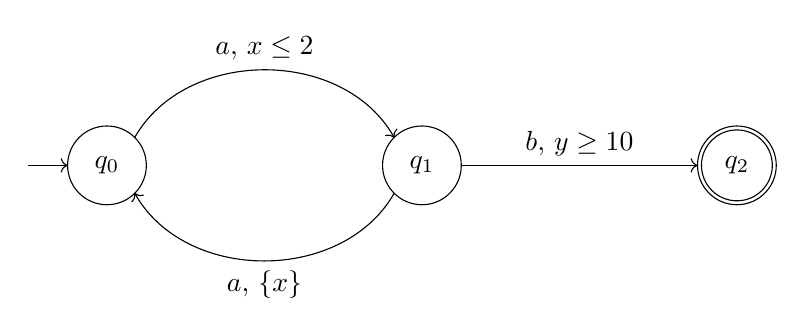
\begin{tikzpicture}[scale=1, every node/.style={transform shape}]

\filldraw [fill=white]  (0,0)  circle (5mm) node (q0) {$q_0$};
\filldraw [fill=white]  (4,0)  circle (5mm) node (q1) {$q_1$};
\filldraw [fill=white]  (8,0)  circle (5mm) node (q2) {$q_2$};
\draw (8,0)  circle (4.5mm);

\begin{scope}[->]
\draw (0.35,0.35) .. controls (1,1.5) and (3,1.5) .. (3.65,0.35) node [midway, above] {$a,\, x \leq 2$};
\draw (3.65,-0.35) .. controls (3,-1.5) and (1,-1.5) .. (0.35,-0.35) node [midway, below] {$a,\, \{x\}$};
\draw (4.5,0) -- (7.5,0) node [midway, above] {$b,\, y \geq 10$};
\draw (-1,0) -- (-0.5,0);
\end{scope}

\end{tikzpicture}
\caption{A timed automaton \(\mathcal{A}_1\). Both clocks \(x\) and \(y\) start at \(0\) in state \(q_0\). The transition on \(a\) from \(q_0\) to \(q_1\) has the guard \(x \leq 2\), forcing the system to spend at most \(2\) time units before taking it. The transition on \(a\) from \(q_1\) to \(q_0\) has no guard and resets \(x\). The guard on \(b\) from \(q_1\) to \(q_2\) requires that at least \(10\) time units have elapsed since the start, via the constraint \(y \geq 10\).}
\label{fig:ab}
\end{figure}

\paragraph{Semantics and State Space.}
A configuration of a timed automaton is a pair \((q,v)\) where \(q\) is a location and \(v\) is a valuation assigning to each clock a non-negative real number. Timed automata have two kinds of transitions:
\begin{itemize}
  \item \emph{Delay transitions}, where time elapses and all clocks increase uniformly.
  \item \emph{Action transitions}, where a guarded transition is fired and some clocks are reset.
\end{itemize}

\begin{figure}[t]
\centering
\begin{tikzpicture}

\node at (0,0) {$(q_0, \langle 0, 0 \rangle)$};
\node at (-4,-2) {$(q_1, \langle 0, 0 \rangle)$};
\node at (0,-2) {$(q_1, \langle 0.8, 0.8 \rangle)$};
\node at (4,-2) {$(q_1, \langle 1.5, 1.5 \rangle)$};
\node at (-4,-4) {$(q_0, \langle 0, 0.8 \rangle)$};
\node at (0,-4) {$(q_0, \langle 0, 5.8 \rangle)$};
\node at (4,-4) {$(q_0, \langle 0, 9.8 \rangle)$};
\node at (0,-6) {$(q_1, \langle 0.5, 10.3 \rangle)$};
\node at (4,-6) {$(q_1, \langle 1.2, 11 \rangle)$};
\node at (8,-6) {$(q_1, \langle 1.8, 11.6  \rangle)$};
\node at (4,-8) {$(q_2, \langle 2.2, 12 \rangle)$};

\node at (-2,-2) {$\cdots$};
\node at (2,-2) {$\cdots$};
\node at (6,-2) {$\cdots$};
\node at (-2,-4) {$\cdots$};
\node at (2,-4) {$\cdots$};
\node at (6,-4) {$\cdots$};
\node at (-2,-6) {$\cdots$};
\node at (2,-6) {$\cdots$};
\node at (6,-6) {$\cdots$};
\node at (10,-6) {$\cdots$};
\node at (2,-8) {$\cdots$};
\node at (6,-8) {$\cdots$};
\node at (-4,-2.5) {$\vdots$};
\node at (4,-2.5) {$\vdots$};
\node at (-4,-4.5) {$\vdots$};
\node at (0,-4.5) {$\vdots$};
\node at (0,-6.5) {$\vdots$};
\node at (8,-6.5) {$\vdots$};

\begin{scope}[-Stealth]
\draw (0,-0.3) -- (-4,-1.7) node [midway, left, above] {\footnotesize $0$};
\draw (0,-0.3) -- (0,-1.7) node [midway, left] {\footnotesize $0.8$};
\draw (0,-0.3) -- (4,-1.7) node [midway, right, above] {\footnotesize $1.5$};
\draw (0,-2.3) -- (-4,-3.7) node [midway, left, above] {\footnotesize $0$};
\draw (0,-2.3) -- (0,-3.7) node [midway, left] {\footnotesize $5$};
\draw (0,-2.3) -- (4,-3.7) node [midway, right, above] {\footnotesize $9$};
\draw (4,-4.3) -- (0,-5.7) node [midway, left, above] {\footnotesize $0.5$};
\draw (4,-4.3) -- (4,-5.7) node [midway, left] {\footnotesize $1.2$};
\draw (4,-4.3) -- (8,-5.7) node [midway, right, above] {\footnotesize $1.8$};
\draw (4,-6.3) -- (4,-7.7) node [midway, left] {\footnotesize $1$};
\end{scope}

\end{tikzpicture}
\caption{Part of the transition system of the timed automaton \(\mathcal{A}_1\), showing several possible runs.}
\label{fig:ab-behavior}
\end{figure}

Figure~\ref{fig:ab-behavior} depicts part of the (infinite) transition system of \(\mathcal{A}_1\), showing some possible configurations and transitions. Starting from the initial configuration \((q_0, \langle 0,0 \rangle)\), the system may let time elapse in \(q_0\) for any duration between \(0\) and \(2\) units before taking the transition on \(a\) to \(q_1\). For instance, after \(0.8\) time units, the clock valuation becomes \(\langle 0.8, 0.8 \rangle\). Once in \(q_1\), the automaton can again delay, and may take the loop on \(a\) (resetting \(x\)) or eventually take the transition on \(b\) when \(y \ge 10\). Different choices of delay durations lead to uncountably many distinct runs.

\paragraph{The Reachability Problem and Its Solutions.}
The \emph{reachability problem} for a timed automaton asks whether there exists a run from the initial state to an accepting state. Reachability has been extensively studied and forms the basis of verification tools such as \textsc{UPPAAL}, \textsc{Kronos}, \textsc{TChecker}, and \textsc{Theta}.

A key difficulty is that the space of clock valuations is uncountable. For any fixed sequence of action transitions, there are uncountably many ways to interleave delays, leading to uncountably many runs. To solve the reachability problem effectively, one must reason symbolically about sets of valuations.

The classical solution relies on a finite partition of the valuation space into equivalence classes called \emph{regions}~\cite{AlurDillTA}. Given a bound function \(M\) that associates to each clock \(x\) the largest constant appearing in any guard involving \(x\), one defines a finite partition where clock valuations in the same region are indistinguishable with respect to reachability. For the automaton \(\mathcal{A}_1\), the maximal bound function \(M_1\) satisfies \(M_1(x) = 2\) and \(M_1(y) = 10\). The \emph{region graph} is then obtained by taking the product of locations with regions. It has been shown that the region graph is sound and complete for reachability~\cite{AlurDillTA}. However, region graphs are often too large to be practical for verification.

In practice, reachability analysis for timed automata is typically based on \emph{zones}~\cite{DillPhD} rather than regions. Zones are convex sets of clock valuations defined by difference constraints of the form \(x - y \bowtie c\). They can be efficiently represented and manipulated using difference bound matrices (DBMs), yielding scalable algorithms. In this thesis, we will rely on regions as a conceptual tool to reason about finiteness and complexity, but our main focus will be on modelling and complexity rather than implementing zone-based algorithms.

\paragraph{Networks of Timed Automata.} Real systems often consist of multiple concurrent components, modeled as networks of timed automata that synchronize on shared actions. In the standard semantics, all automata share a global time, and their clocks advance synchronously. This global-time assumption simplifies some aspects of verification but obscures potential independence between components.

\subsection{Negotiations}
\label{subsubsec:negotiations}

Where timed automata focus on individual agents with timing constraints, \emph{negotiations}~\cite{EsparzaDeselNegotiations} provide a model of concurrency centered on multiparty synchronization. A negotiation structures workflow as atomic multiparty interactions. We give an informal description here; the precise definition is recalled in Chapter \ref{chap:preliminaries}. A multiparty \emph{atomic negotiation} involves a set of \emph{processes} (or \emph{agents}) jointly choosing an outcome from a finite set. Esparza and Desel introduced \emph{distributed negotiations} (or simply \emph{negotiations})~\cite{EsparzaDeselNegotiations} as a model of concurrency where such atomic negotiations are the basic building blocks. A negotiation structures a workflow of atomic negotiations: after each atomic negotiation, participating agents agree on an outcome and move to subsequent atomic negotiations as prescribed by the workflow.

This makes concurrency explicit: nodes involving disjoint sets of processes can occur independently (true concurrency), while nodes requiring common participants enforce synchronization. Unlike Petri nets, which encode multiparty synchronization indirectly through places and transitions, negotiations take atomic multiparty interaction as a primitive concept.

Graphically, negotiations resemble Petri nets. Nodes appear as black bars. For each participating process, a white circle (a \emph{port}) sits on the bar. The set of participating processes is the node's \emph{domain}. Each node has outgoing \emph{outcomes} represented by arrows. For each outcome $r$ and each process $p$ in the domain, the negotiation specifies which nodes $p$ becomes ready to participate in next if $r$ is chosen. When outcomes lead to multiple possibilities for a single process, we use \emph{hyperarcs} (branching arrows) to represent non-determinism.

\begin{figure}[t]
\centering
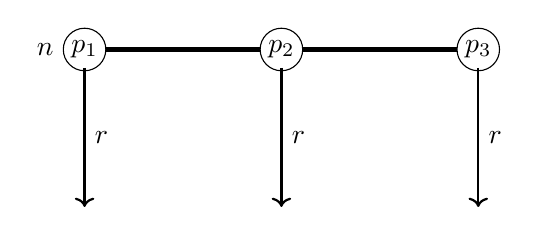
\begin{tikzpicture}

\begin{scope}[line width=2pt]
\draw (0,0) node at (-0.5,0) {$n$} -- (5,0);
\end{scope}

\begin{scope}[fill=white]
\filldraw  (0,0)  circle (2.7mm) node (nic) {$p_1$};
\filldraw  (2.5,0)  circle (2.7mm) node (nia) {$p_2$};
\filldraw  (5,0)  circle (2.7mm) node (nib) {$p_3$};
\end{scope}

\begin{scope}[thick,->]

\draw (nic) -- (0,-2) node [right, midway] {$r$};
\draw (nia) -- (2.5,-2) node [right, midway] {$r$};
\draw (nib) -- (5,-2) node [right, midway] {$r$};
\end{scope}

\end{tikzpicture}
\caption{A simple node $n$ with three processes $\{p_1, p_2, p_3\}$ in its domain, and the set of outcomes is $\{r\}$}
\label{fig:node}
\end{figure}

\subsubsection{A simple example: ATM workflow}
\label{example:ATM-untimed}

Before presenting a more elaborate scenario, we introduce negotiations through a simple example. Consider a transaction in an ATM machine ($a$), where a customer ($c$) wants to withdraw money from her bank ($b$).  Here, $a$, $c$, and $b$ are the \emph{processes} in the system. Their direct interactions are represented by thick horizontal lines (nodes). After each interaction, the participating agents decide on an outcome, represented by arrows. Initially, all agents are in the node $n_{in}$ node. They choose the outcome $st$ to start the transaction. Agents $a$ and $c$ go to node $n_1$ and $b$ goes to $n_2$.The customer gives her card details and requests for money withdrawal in the ATM at node $n_1$ by the outcome $req$. At $n_2$, the ATM conveys this request to the bank and sends the details through the outcome $det$. All three processes talk to each other at $n_3$, where the bank checks if there is sufficient money in the account and let the customer know via the ATM. They select $ok$ if the transaction is approved and go to $n_f$ otherwise they go back to $n_{in}$ by choosing the outcome $fail$.

\begin{figure}[t]
\centering
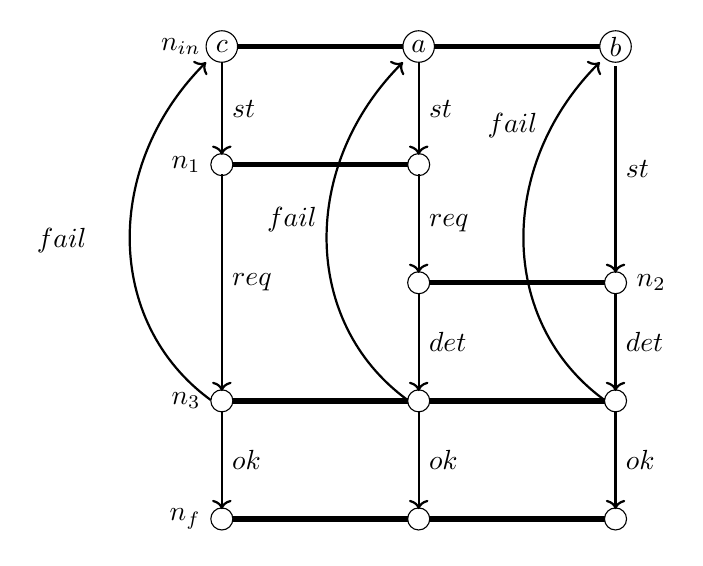
\begin{tikzpicture}

\begin{scope}[line width=2pt]
\draw (0.,0) node [left] {$n_{in}\,\,$} -- (5,0);
\draw (0.,-1.5) node [left] {$n_{1}\,\,$} -- (2.5,-1.5);
\draw (2.5,-3) -- (5,-3) node [right] {$\,\,n_{2}$};
\draw (0.,-4.5) node [left] {$n_{3}\,\,$} -- (5,-4.5);
\draw (0.,-6) node [left] {$n_{f}\,\,$} -- (5,-6);
\end{scope}

\begin{scope}[fill=white]
\filldraw  (0,0)  circle (2mm) node (nic) {$c$};
\filldraw  (2.5,0)  circle (2mm) node (nia) {$a$};
\filldraw  (5,0)  circle (2mm) node (nib) {$b$};

\filldraw  (0,-1.5)  circle (1.4mm) node (n1c) {};
\filldraw  (2.5,-1.5)  circle (1.4mm) node (n1a) {};

\filldraw  (2.5,-3)  circle (1.4mm) node (n2a) {};
\filldraw  (5,-3)  circle (1.4mm) node (n2b) {};

\filldraw  (0,-4.5)  circle (1.4mm) node (n3c) {};
\filldraw  (2.5,-4.5)  circle (1.4mm) node (n3a) {};
\filldraw  (5,-4.5)  circle (1.4mm) node (n3b) {};

\filldraw  (0,-6)  circle (1.4mm) node (n4c) {};
\filldraw  (2.5,-6)  circle (1.4mm) node (n4a) {};
\filldraw  (5,-6)  circle (1.4mm) node (n4b) {};
\end{scope}

\begin{scope}[thick,->]

\draw (nic) -- (n1c) node [right, midway] {$st$};
\draw (n1c) -- (n3c) node [right, midway] {$req$};
\draw (n3c) -- (n4c) node [right, midway] {$ok$};

\draw (nia) -- (n1a) node [right, midway] {$st$};
\draw (n1a) -- (n2a) node [right, midway] {$req$};
\draw (n2a) -- (n3a) node [right, midway] {$det$};
\draw (n3a) -- (n4a) node [right, midway] {$ok$};

\draw (nib) -- (n2b) node [right, midway] {$st$};
\draw (n2b) -- (n3b) node [right, midway] {$det$};
\draw (n3b) -- (n4b) node [right, midway] {$ok$};

\draw (n3c) + (-0.14,0.01) .. controls  (-1.5,-3.5) and (-1.5,-1.5) .. (nic) node [left=-0.2cm, text width = 1.25 cm, midway] {$fail$};
\draw (n3a) + (-0.14,0.01) .. controls  (1,-3.5) and (1,-1.5) .. (nia) node at (1.2,-2.2) [text width = 1.25 cm] {$fail$};
\draw (n3b) + (-0.14,0.01) .. controls  (3.5,-3.5) and (3.5,-1.5) .. (nib) node at (4,-1) [text width = 1.25 cm] {$fail$};

\end{scope}

\end{tikzpicture}
\caption{A distributed negotiations modelling a transaction between a customer, an ATM and a bank}
\label{fig:ATM}
\end{figure}


\begin{figure}[t]
\centering
\tikzset{every picture/.style={line width=0.75pt}} %set default line width to 0.75pt        

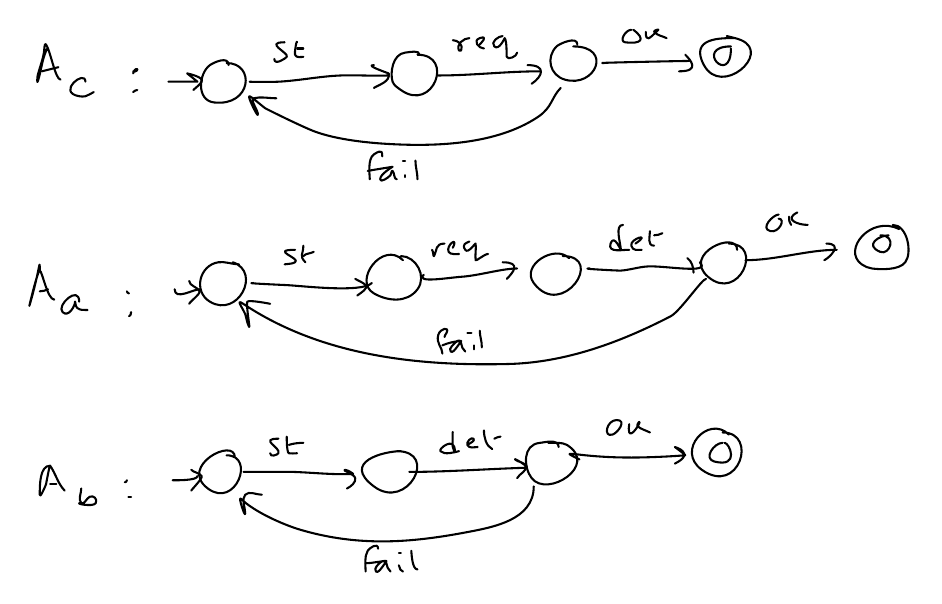
\begin{tikzpicture}[x=0.75pt,y=0.75pt,yscale=-1,xscale=1]
%uncomment if require: \path (0,300); %set diagram left start at 0, and has height of 300

%Shape: Free Drawing [id:dp699352073377679] 
\draw  [line width=0.75] [line join = round][line cap = round] (126,35) .. controls (126,30.35) and (118.72,33.77) .. (117,35) .. controls (111.56,38.89) and (110.28,52.03) .. (119,53) .. controls (137.12,55.01) and (139.04,34) .. (125,34) ;
%Shape: Free Drawing [id:dp20910792466845673] 
\draw  [line width=0.75] [line join = round][line cap = round] (218,30) .. controls (218,27.64) and (213.34,28.74) .. (211,29) .. controls (204.97,29.67) and (203.65,38.95) .. (205,43) .. controls (205.6,44.79) and (207.47,45.9) .. (209,47) .. controls (224.54,58.1) and (235.01,30) .. (217,30) ;
%Shape: Free Drawing [id:dp5846892232392498] 
\draw  [line width=0.75] [line join = round][line cap = round] (294,25) .. controls (294,20.83) and (285.31,24.69) .. (284,26) .. controls (278.68,31.32) and (280.76,39.93) .. (288,42) .. controls (302.83,46.24) and (311.37,26) .. (292,26) ;
%Shape: Free Drawing [id:dp6112448648060961] 
\draw  [line width=0.75] [line join = round][line cap = round] (370,22) .. controls (363.6,22) and (347.75,21.54) .. (355,35) .. controls (363.4,50.61) and (387.73,29.54) .. (373,23) .. controls (370.78,22.01) and (368.33,21.67) .. (366,21) ;
%Shape: Free Drawing [id:dp42021497143682085] 
\draw  [line width=0.75] [line join = round][line cap = round] (131,131) .. controls (127.65,131) and (124.31,129.49) .. (121,130) .. controls (111.93,131.4) and (108.77,144.06) .. (117,149) .. controls (130.47,157.08) and (142,134.67) .. (128,130) ;
%Shape: Free Drawing [id:dp9428654622094055] 
\draw  [line width=0.75] [line join = round][line cap = round] (210,129) .. controls (200.27,119.27) and (185.6,139.06) .. (196,145) .. controls (202.5,148.72) and (211.86,149.86) .. (217,143) .. controls (221.71,136.72) and (216.23,127) .. (209,127) ;
%Shape: Free Drawing [id:dp22523578617590523] 
\draw  [line width=0.75] [line join = round][line cap = round] (290,128) .. controls (283.18,121.18) and (266.55,131.4) .. (273,140) .. controls (286.56,158.09) and (307.8,127) .. (287,127) ;
%Shape: Free Drawing [id:dp6357001104153978] 
\draw  [line width=0.75] [line join = round][line cap = round] (371,124) .. controls (371,114.33) and (344.11,125.95) .. (357,137) .. controls (371.74,149.63) and (384.24,121) .. (367,121) ;
%Shape: Free Drawing [id:dp43290352630083795] 
\draw  [line width=0.75] [line join = round][line cap = round] (449,114) .. controls (435.4,107.2) and (421.33,124.09) .. (431,131) .. controls (432.46,132.04) and (434.22,132.76) .. (436,133) .. controls (439.62,133.48) and (449.01,133.98) .. (452,130) .. controls (455.53,125.3) and (452.98,112) .. (446,112) ;
%Shape: Free Drawing [id:dp4854772884625288] 
\draw  [line width=0.75] [line join = round][line cap = round] (129,224) .. controls (129,214.07) and (101.58,228.19) .. (116,239) .. controls (129.38,249.03) and (139.18,223) .. (125,223) ;
%Shape: Free Drawing [id:dp3971045256545481] 
\draw  [line width=0.75] [line join = round][line cap = round] (209,221) .. controls (200.93,221) and (180.13,226.1) .. (196,238) .. controls (212.1,250.07) and (227.59,221) .. (207,221) ;
%Shape: Free Drawing [id:dp4509421284855678] 
\draw  [line width=0.75] [line join = round][line cap = round] (285,219) .. controls (285,214.88) and (278.13,216.81) .. (276,217) .. controls (267.43,217.78) and (268.11,229) .. (272,234) .. controls (279.6,243.78) and (304.55,227.72) .. (289,218) .. controls (286.75,216.6) and (282.29,217) .. (280,217) ;
%Shape: Free Drawing [id:dp24931842316411212] 
\draw  [line width=0.75] [line join = round][line cap = round] (367,213) .. controls (357.27,203.27) and (341.05,220.75) .. (354,230) .. controls (371.89,242.78) and (381.31,212) .. (364,212) ;
%Shape: Free Drawing [id:dp9658349676228442] 
\draw  [line width=0.75] [line join = round][line cap = round] (39,27) .. controls (39,25.51) and (37.42,29.57) .. (37,31) .. controls (35.84,34.96) and (35.3,39.09) .. (34,43) .. controls (33.68,43.95) and (33.76,40.97) .. (34,40) .. controls (34.97,36.11) and (36.35,32.93) .. (37,29) .. controls (37.23,27.64) and (37.24,23.86) .. (38,25) .. controls (40.19,28.28) and (42.53,42) .. (45,42) ;
%Shape: Free Drawing [id:dp09004794014509787] 
\draw  [line width=0.75] [line join = round][line cap = round] (36,38) .. controls (38.67,37.33) and (41.33,36.67) .. (44,36) ;
%Shape: Free Drawing [id:dp6821526471402938] 
\draw  [line width=0.75] [line join = round][line cap = round] (57,43) .. controls (57,36.82) and (42.78,48.13) .. (54,50) .. controls (54.99,50.16) and (56.04,50.27) .. (57,50) .. controls (58.43,49.59) and (59.67,48.67) .. (61,48) ;
%Shape: Free Drawing [id:dp19914947748820078] 
\draw  [line width=0.75] [line join = round][line cap = round] (80,38) .. controls (80,38.75) and (82.53,37.53) .. (82,37) .. controls (81.33,36.33) and (80,38.06) .. (80,39) ;
%Shape: Free Drawing [id:dp22950086205936715] 
\draw  [line width=0.75] [line join = round][line cap = round] (80,48) .. controls (80.53,47.47) and (81.25,47) .. (82,47) ;
%Shape: Free Drawing [id:dp8458179935856099] 
\draw  [line width=0.75] [line join = round][line cap = round] (35,134) .. controls (35,126.72) and (35.09,133.7) .. (30,151) .. controls (29.68,152.08) and (33.95,134) .. (35,134) .. controls (36.12,134) and (38.71,148) .. (42,148) ;
%Shape: Free Drawing [id:dp8709509858246236] 
\draw  [line width=0.75] [line join = round][line cap = round] (35,144) .. controls (36.37,144) and (37.77,143.61) .. (39,143) ;
%Shape: Free Drawing [id:dp1689306225658136] 
\draw  [line width=0.75] [line join = round][line cap = round] (54,149) .. controls (54,140.69) and (42.78,150.78) .. (46,154) .. controls (48.77,156.77) and (52,151.14) .. (52,149) .. controls (52,147.95) and (52.16,151.37) .. (53,152) .. controls (54.61,153.21) and (56.22,153) .. (58,153) ;
%Shape: Free Drawing [id:dp9154214496730456] 
\draw  [line width=0.75] [line join = round][line cap = round] (77,144) .. controls (77,144.47) and (77.53,145) .. (78,145) ;
%Shape: Free Drawing [id:dp0780602300217802] 
\draw  [line width=0.75] [line join = round][line cap = round] (78,156) .. controls (78.75,156) and (79,154.75) .. (79,154) ;
%Shape: Free Drawing [id:dp8104400124521838] 
\draw  [line width=0.75] [line join = round][line cap = round] (40,228) .. controls (35.04,228) and (35,237.04) .. (35,242) .. controls (35,243.94) and (37.32,238.82) .. (38,237) .. controls (38.1,236.73) and (39.71,227.58) .. (40,228) .. controls (42.66,231.79) and (43.73,236.73) .. (47,240) ;
%Shape: Free Drawing [id:dp1836175709335458] 
\draw  [line width=0.75] [line join = round][line cap = round] (40,237) .. controls (41,237) and (42,237) .. (43,237) ;
%Shape: Free Drawing [id:dp5761019515015455] 
\draw  [line width=0.75] [line join = round][line cap = round] (55,239) .. controls (55,241.33) and (53.35,244.35) .. (55,246) .. controls (56.18,247.18) and (57.51,243.75) .. (59,243) .. controls (60.91,242.05) and (62.95,244.09) .. (62,246) .. controls (60.9,248.19) and (50.6,246) .. (55,246) ;
%Shape: Free Drawing [id:dp11510509263160207] 
\draw  [line width=0.75] [line join = round][line cap = round] (76,236) .. controls (76.47,236) and (77,235.47) .. (77,235) ;
%Shape: Free Drawing [id:dp1326029043307244] 
\draw  [line width=0.75] [line join = round][line cap = round] (78,243) .. controls (76.79,243) and (77.96,243) .. (79,243) ;
%Shape: Free Drawing [id:dp47687509882848156] 
\draw  [line width=0.75] [line join = round][line cap = round] (100,43) .. controls (88.71,43) and (111,43) .. (111,43) .. controls (111,43) and (106,39) .. (106,39) .. controls (106,39) and (114.38,40.7) .. (113,43) .. controls (112.03,44.62) and (110.33,45.67) .. (109,47) ;
%Shape: Free Drawing [id:dp2442975775805618] 
\draw  [line width=0.75] [line join = round][line cap = round] (100,143) .. controls (100,148.52) and (108.95,143) .. (112,143) ;
%Shape: Free Drawing [id:dp3598381417417724] 
\draw  [line width=0.75] [line join = round][line cap = round] (107,139) .. controls (107,141.36) and (111.07,141.83) .. (112,144) .. controls (112.49,145.15) and (107.59,148.82) .. (107,150) ;
%Shape: Free Drawing [id:dp7335814100329172] 
\draw  [line width=0.75] [line join = round][line cap = round] (99,235) .. controls (99.04,235) and (111,235.38) .. (111,233) ;
%Shape: Free Drawing [id:dp3988930161980966] 
\draw  [line width=0.75] [line join = round][line cap = round] (108,230) .. controls (109.37,231.37) and (111.92,231.38) .. (113,233) .. controls (113.63,233.95) and (108.75,238.88) .. (108,240) ;
%Shape: Free Drawing [id:dp5504071776051671] 
\draw  [line width=0.75] [line join = round][line cap = round] (137,43) .. controls (132.67,43) and (145.67,43.23) .. (150,43) .. controls (159.94,42.48) and (170.09,40.37) .. (180,40) .. controls (187.66,39.72) and (195.34,40.33) .. (203,40) .. controls (203.33,39.99) and (203.33,39) .. (203,39) ;
%Shape: Free Drawing [id:dp38092617558048913] 
\draw  [line width=0.75] [line join = round][line cap = round] (196,35) .. controls (191.21,35) and (202.94,38.83) .. (203,39) .. controls (204.31,42.93) and (197.91,44.64) .. (196,46) ;
%Shape: Free Drawing [id:dp3455480331109182] 
\draw  [line width=0.75] [line join = round][line cap = round] (227,40) .. controls (243.44,40) and (259.78,38) .. (276,38) ;
%Shape: Free Drawing [id:dp0471808156338025] 
\draw  [line width=0.75] [line join = round][line cap = round] (270,35) .. controls (279.42,35) and (277.22,40.52) .. (272,44) ;
%Shape: Free Drawing [id:dp03599926708867218] 
\draw  [line width=0.75] [line join = round][line cap = round] (307,34) .. controls (298.31,34) and (343.84,33) .. (348,33) ;
%Shape: Free Drawing [id:dp60137065125319] 
\draw  [line width=0.75] [line join = round][line cap = round] (346,30) .. controls (348.43,32.43) and (353.55,38) .. (343,38) ;
%Shape: Free Drawing [id:dp6317644494836507] 
\draw  [line width=0.75] [line join = round][line cap = round] (286,46) .. controls (281.46,50.54) and (281.99,55.34) .. (275,60) .. controls (255.09,73.27) and (226.16,74.32) .. (203,73) .. controls (191.49,72.34) and (175.52,70.6) .. (165,66) .. controls (157.9,62.89) and (150.93,59.47) .. (144,56) .. controls (142.76,55.38) and (136.92,50) .. (136,50) .. controls (134.93,50) and (139.75,59.5) .. (140,59) .. controls (140.75,57.5) and (136,51.55) .. (138,51) .. controls (141.54,50.04) and (145.33,51) .. (149,51) ;
%Shape: Free Drawing [id:dp5041132373888955] 
\draw  [line width=0.75] [line join = round][line cap = round] (153,24) .. controls (142.74,24) and (155.35,29.2) .. (154,31) .. controls (153.34,31.88) and (148,35.38) .. (148,32) ;
%Shape: Free Drawing [id:dp9052641536236868] 
\draw  [line width=0.75] [line join = round][line cap = round] (159,24) .. controls (159,21.97) and (157.67,28) .. (158,30) .. controls (158.28,31.71) and (161.55,31) .. (162,31) ;
%Shape: Free Drawing [id:dp00037039861442378363] 
\draw  [line width=0.75] [line join = round][line cap = round] (159,27) .. controls (160,27) and (161,27) .. (162,27) ;
%Shape: Free Drawing [id:dp3222100625858557] 
\draw  [line width=0.75] [line join = round][line cap = round] (234,23) .. controls (236.36,23) and (239.38,25.24) .. (238,28) .. controls (237.85,28.3) and (237.15,28.3) .. (237,28) .. controls (235.48,24.97) and (239.25,22) .. (242,22) ;
%Shape: Free Drawing [id:dp8528288775510539] 
\draw  [line width=0.75] [line join = round][line cap = round] (247,25) .. controls (247.37,24.63) and (251.6,20.47) .. (247,22) .. controls (243.41,23.2) and (246.47,27) .. (249,27) ;
%Shape: Free Drawing [id:dp6245891639619918] 
\draw  [line width=0.75] [line join = round][line cap = round] (258,21) .. controls (256.1,21) and (251.91,23.91) .. (254,26) .. controls (256.19,28.19) and (259,22) .. (259,22) .. controls (260.08,23.08) and (259.88,30.4) .. (260,31) .. controls (260.35,32.76) and (265,30.8) .. (265,29) ;
%Shape: Free Drawing [id:dp2955298345225923] 
\draw  [line width=0.75] [line join = round][line cap = round] (320,18) .. controls (317.07,18) and (314.05,23.63) .. (317,24) .. controls (324.7,24.96) and (327.28,22.71) .. (321,18) ;
%Shape: Free Drawing [id:dp7650219261943041] 
\draw  [line width=0.75] [line join = round][line cap = round] (327,19) .. controls (327,24.19) and (328.59,22.41) .. (333,18) .. controls (333.53,17.47) and (330.47,18.47) .. (331,19) .. controls (333.05,21.05) and (334.69,20.84) .. (337,22) ;
%Shape: Free Drawing [id:dp9858048471107251] 
\draw  [line width=0.75] [line join = round][line cap = round] (200,79) .. controls (200,77.39) and (200.33,75.11) .. (196,78) .. controls (192.81,80.13) and (194,88.12) .. (194,90) ;
%Shape: Free Drawing [id:dp27682562555764234] 
\draw  [line width=0.75] [line join = round][line cap = round] (193,86) .. controls (194.11,85.72) and (205,84) .. (205,84) .. controls (205,84) and (199,87.47) .. (199,90) .. controls (199,91.8) and (202.88,89.4) .. (204,88) .. controls (204.47,87.42) and (204.47,85.47) .. (205,86) .. controls (206.05,87.05) and (205.51,90) .. (207,90) ;
%Shape: Free Drawing [id:dp9843351866594481] 
\draw  [line width=0.75] [line join = round][line cap = round] (211,88) .. controls (211,88.33) and (211,88.67) .. (211,89) ;
%Shape: Free Drawing [id:dp7139829189684593] 
\draw  [line width=0.75] [line join = round][line cap = round] (211,81) .. controls (209.67,81) and (209.67,81) .. (211,81) ;
%Shape: Free Drawing [id:dp9021117212192773] 
\draw  [line width=0.75] [line join = round][line cap = round] (216,81) .. controls (216,84.02) and (217,86.98) .. (217,90) ;
%Shape: Free Drawing [id:dp44700280018755034] 
\draw  [line width=0.75] [line join = round][line cap = round] (368,26) .. controls (349.6,26) and (368,45.62) .. (368,27) ;
%Shape: Free Drawing [id:dp36075313476514703] 
\draw  [line width=0.75] [line join = round][line cap = round] (138,140) .. controls (132.66,140) and (148.66,140.76) .. (154,141) .. controls (160.98,141.32) and (190.11,144.89) .. (195,140) ;
%Shape: Free Drawing [id:dp6900079518028266] 
\draw  [line width=0.75] [line join = round][line cap = round] (187,138) .. controls (188.67,139) and (190.63,139.63) .. (192,141) .. controls (193.51,142.51) and (189.71,144.72) .. (188,146) ;
%Shape: Free Drawing [id:dp857009029163824] 
\draw  [line width=0.75] [line join = round][line cap = round] (220,136) .. controls (215.75,140.25) and (232,137.4) .. (238,137) .. controls (246.64,136.42) and (257.64,133) .. (265,133) ;
%Shape: Free Drawing [id:dp7791873524744648] 
\draw  [line width=0.75] [line join = round][line cap = round] (258,130) .. controls (267.22,130) and (263.14,134.86) .. (260,138) ;
%Shape: Free Drawing [id:dp030091329506495068] 
\draw  [line width=0.75] [line join = round][line cap = round] (300,133) .. controls (293.94,133) and (313.66,134.09) .. (315,134) .. controls (319.37,133.7) and (323.62,132.22) .. (328,132) .. controls (336.35,131.57) and (358.91,135.91) .. (353,130) ;
%Shape: Free Drawing [id:dp6794109558694876] 
\draw  [line width=0.75] [line join = round][line cap = round] (347,128) .. controls (349.11,129.41) and (350,132.46) .. (350,135) ;
%Shape: Free Drawing [id:dp4941635414386235] 
\draw  [line width=0.75] [line join = round][line cap = round] (158,124) .. controls (145.53,124) and (161.16,128.1) .. (158,130) .. controls (156.54,130.87) and (154.67,130.67) .. (153,131) ;
%Shape: Free Drawing [id:dp08363776027723879] 
\draw  [line width=0.75] [line join = round][line cap = round] (162,122) .. controls (162,126.3) and (159.8,126.8) .. (163,130) ;
%Shape: Free Drawing [id:dp17133608241358922] 
\draw  [line width=0.75] [line join = round][line cap = round] (162,127) .. controls (163.43,125.57) and (165.08,125.96) .. (167,125) ;
%Shape: Free Drawing [id:dp42444576991187455] 
\draw  [line width=0.75] [line join = round][line cap = round] (224,124) .. controls (224.75,124.75) and (224.53,127.94) .. (225,127) .. controls (226.45,124.11) and (225.48,121) .. (230,121) ;
%Shape: Free Drawing [id:dp42354377365438856] 
\draw  [line width=0.75] [line join = round][line cap = round] (234,123) .. controls (236.99,117.03) and (230.46,121.93) .. (232,125) .. controls (232.72,126.45) and (236.17,126) .. (237,126) ;
%Shape: Free Drawing [id:dp254637723356695] 
\draw  [line width=0.75] [line join = round][line cap = round] (242,120) .. controls (240.5,120.75) and (238.13,121.19) .. (240,124) .. controls (241.41,126.12) and (244.93,120.44) .. (245,121) .. controls (245.33,123.65) and (244.67,126.35) .. (245,129) .. controls (245.09,129.7) and (249.25,126) .. (251,126) ;
%Shape: Free Drawing [id:dp8660053496027834] 
\draw  [line width=0.75] [line join = round][line cap = round] (316,112) .. controls (311.99,112) and (314.67,120) .. (315,124) .. controls (315.06,124.76) and (311.71,115.88) .. (310,121) .. controls (308.39,125.84) and (316.64,123.74) .. (319,124) ;
%Shape: Free Drawing [id:dp5631701100684178] 
\draw  [line width=0.75] [line join = round][line cap = round] (322,121) .. controls (330.22,115.52) and (319.15,118.59) .. (320,122) .. controls (320.68,124.71) and (323.21,124) .. (325,124) ;
%Shape: Free Drawing [id:dp05369272016552906] 
\draw  [line width=0.75] [line join = round][line cap = round] (329,115) .. controls (329,117.48) and (327.44,122) .. (331,122) ;
%Shape: Free Drawing [id:dp7255991302691805] 
\draw  [line width=0.75] [line join = round][line cap = round] (331,117) .. controls (332.37,117) and (333.77,116.61) .. (335,116) ;
%Shape: Free Drawing [id:dp26821501258625524] 
\draw  [line width=0.75] [line join = round][line cap = round] (375,129) .. controls (389.77,129) and (404.91,124) .. (419,124) ;
%Shape: Free Drawing [id:dp19135576727743342] 
\draw  [line width=0.75] [line join = round][line cap = round] (414,121) .. controls (422.3,121) and (415.75,127.63) .. (413,129) ;
%Shape: Free Drawing [id:dp9970516135074035] 
\draw  [line width=0.75] [line join = round][line cap = round] (391,107) .. controls (388.45,107) and (381.8,113.7) .. (387,115) .. controls (391.11,116.03) and (394.61,109) .. (391,109) ;
%Shape: Free Drawing [id:dp7586304194815168] 
\draw  [line width=0.75] [line join = round][line cap = round] (396,108) .. controls (396,109.37) and (396.03,111.03) .. (397,112) ;
%Shape: Free Drawing [id:dp011025846487307756] 
\draw  [line width=0.75] [line join = round][line cap = round] (400,106) .. controls (393.21,109.39) and (400.38,112) .. (405,112) ;
%Shape: Free Drawing [id:dp19856863207902364] 
\draw  [line width=0.75] [line join = round][line cap = round] (444,117) .. controls (439.43,117) and (431.97,121.79) .. (440,125) .. controls (444.48,126.79) and (448.25,117) .. (440,117) ;
%Shape: Free Drawing [id:dp8137485876937424] 
\draw  [line width=0.75] [line join = round][line cap = round] (356,138) .. controls (354.11,138) and (343.46,153.69) .. (339,156) .. controls (314.76,168.54) and (288.51,178.29) .. (261,179) .. controls (216.71,180.14) and (170.45,174.97) .. (133,150) .. controls (129.25,147.5) and (132.38,151.36) .. (134,155) .. controls (134.56,156.26) and (134.49,157.72) .. (135,159) .. controls (135.28,159.69) and (136,161.75) .. (136,161) .. controls (136,160.05) and (134.32,149.68) .. (135,149) .. controls (136,148) and (145.68,149.95) .. (146,150) ;
%Shape: Free Drawing [id:dp670488850721851] 
\draw  [line width=0.75] [line join = round][line cap = round] (230,166) .. controls (230,165.25) and (230.67,164.67) .. (231,164) .. controls (232.62,160.77) and (227.92,161.78) .. (227,165) .. controls (225.8,169.21) and (229,170.78) .. (229,174) ;
%Shape: Free Drawing [id:dp3729587461127226] 
\draw  [line width=0.75] [line join = round][line cap = round] (229,170) .. controls (231.85,168.86) and (234.93,168) .. (238,168) .. controls (238.67,168) and (236.47,167.53) .. (236,168) .. controls (234.63,169.37) and (231.63,171.63) .. (233,173) .. controls (234.51,174.51) and (238,166.87) .. (238,169) .. controls (238,170.49) and (238.95,171.95) .. (240,173) ;
%Shape: Free Drawing [id:dp5973208170734658] 
\draw  [line width=0.75] [line join = round][line cap = round] (244,170) .. controls (244,170.67) and (244,171.33) .. (244,172) ;
%Shape: Free Drawing [id:dp6273152642236075] 
\draw  [line width=0.75] [line join = round][line cap = round] (241,164) .. controls (241.67,164) and (242.33,164) .. (243,164) ;
%Shape: Free Drawing [id:dp2664250327058062] 
\draw  [line width=0.75] [line join = round][line cap = round] (247,163) .. controls (247,165.89) and (248,167.48) .. (248,171) ;
%Shape: Free Drawing [id:dp09767215156309195] 
\draw  [line width=0.75] [line join = round][line cap = round] (135,231) .. controls (125.32,231) and (157,231) .. (157,231) .. controls (166.67,231.32) and (176.34,232.44) .. (186,232) .. controls (186.33,231.98) and (183.28,230) .. (182,230) .. controls (179.87,230) and (186.58,231.91) .. (187,234) .. controls (187.42,236.09) and (184.91,238.05) .. (183,239) ;
%Shape: Free Drawing [id:dp4557189487035944] 
\draw  [line width=0.75] [line join = round][line cap = round] (213,231) .. controls (231.28,231) and (250.84,229.57) .. (269,229) .. controls (271.63,228.92) and (262.95,223.95) .. (264,225) .. controls (265.37,226.37) and (268.39,226.16) .. (269,228) .. controls (269.96,230.87) and (266.19,231.63) .. (265,234) ;
%Shape: Free Drawing [id:dp04523814859365094] 
\draw  [line width=0.75] [line join = round][line cap = round] (295,225) .. controls (283.05,219.03) and (293.86,224.8) .. (326,224) .. controls (332.67,223.83) and (339.34,223.51) .. (346,223) .. controls (346.37,222.97) and (341,219) .. (341,219) .. controls (341,219) and (351.22,221.89) .. (341,227) ;
%Shape: Free Drawing [id:dp43397584755084206] 
\draw  [line width=0.75] [line join = round][line cap = round] (150,215) .. controls (140.29,215) and (151.32,219.35) .. (150,222) .. controls (149.69,222.62) and (146,224.29) .. (146,222) ;
%Shape: Free Drawing [id:dp7766950236050176] 
\draw  [line width=0.75] [line join = round][line cap = round] (154,215) .. controls (154,210.61) and (153.76,221.69) .. (155,222) .. controls (156.29,222.32) and (157.67,222) .. (159,222) ;
%Shape: Free Drawing [id:dp8010900191079826] 
\draw  [line width=0.75] [line join = round][line cap = round] (155,218) .. controls (157.24,217.25) and (159.64,217) .. (162,217) ;
%Shape: Free Drawing [id:dp3926412888334434] 
\draw  [line width=0.75] [line join = round][line cap = round] (234,212) .. controls (234,209.67) and (233.77,216.68) .. (234,219) .. controls (234.07,219.74) and (235,221.75) .. (235,221) .. controls (235,213.4) and (226.94,219.94) .. (228,221) .. controls (230,223) and (234.87,221.53) .. (237,221) ;
%Shape: Free Drawing [id:dp1463435029012543] 
\draw  [line width=0.75] [line join = round][line cap = round] (241,218) .. controls (242.18,217.22) and (245,216) .. (244,215) .. controls (242.98,213.98) and (240.33,216.67) .. (241,218) .. controls (241.97,219.94) and (244.28,219) .. (246,219) ;
%Shape: Free Drawing [id:dp14438813709444898] 
\draw  [line width=0.75] [line join = round][line cap = round] (249,211) .. controls (249,214.28) and (250.06,218.53) .. (253,220) ;
%Shape: Free Drawing [id:dp6870409972621128] 
\draw  [line width=0.75] [line join = round][line cap = round] (254,215) .. controls (254.94,214.53) and (255.95,214) .. (257,214) ;
%Shape: Free Drawing [id:dp6342421719103655] 
\draw  [line width=0.75] [line join = round][line cap = round] (313,206) .. controls (308.03,206) and (306.28,214.57) .. (311,213) .. controls (313.49,212.17) and (318.07,206) .. (313,206) -- cycle ;
%Shape: Free Drawing [id:dp46663802286189726] 
\draw  [line width=0.75] [line join = round][line cap = round] (319,208) .. controls (319,209.33) and (318.4,210.81) .. (319,212) .. controls (320.13,214.27) and (324,207.98) .. (324,207) .. controls (324,206.25) and (322.43,208.52) .. (323,209) .. controls (324.72,210.43) and (327,211) .. (329,212) ;
%Shape: Free Drawing [id:dp21435444815750926] 
\draw  [line width=0.75] [line join = round][line cap = round] (273,238) .. controls (273,254.24) and (253.22,257.67) .. (241,260) .. controls (213.34,265.27) and (188.57,267) .. (161,259) .. controls (151.75,256.32) and (137.84,249.84) .. (132,244) .. controls (130.28,242.28) and (134,253.43) .. (134,251) .. controls (134,248) and (132.01,244.24) .. (134,242) .. controls (135.77,240.01) and (139.33,242) .. (142,242) ;
%Shape: Free Drawing [id:dp49544639169575677] 
\draw  [line width=0.75] [line join = round][line cap = round] (198,268) .. controls (198,264.62) and (193.72,267.79) .. (193,269) .. controls (191.26,271.9) and (192,276.08) .. (192,279) ;
%Shape: Free Drawing [id:dp7435150702646659] 
\draw  [line width=0.75] [line join = round][line cap = round] (192,275) .. controls (195.57,275) and (198.37,274) .. (202,274) .. controls (202.67,274) and (200.57,273.66) .. (200,274) .. controls (198.33,275) and (195.63,277.63) .. (197,279) .. controls (198.51,280.51) and (202,272.87) .. (202,275) .. controls (202,276.49) and (202.95,277.95) .. (204,279) ;
%Shape: Free Drawing [id:dp14850568602306735] 
\draw  [line width=0.75] [line join = round][line cap = round] (208,276) .. controls (208.75,277.51) and (208.55,279) .. (210,279) ;
%Shape: Free Drawing [id:dp44143806738856406] 
\draw  [line width=0.75] [line join = round][line cap = round] (208,270) .. controls (208.33,270) and (208.67,270) .. (209,270) ;
%Shape: Free Drawing [id:dp9803674578133618] 
\draw  [line width=0.75] [line join = round][line cap = round] (214,269) .. controls (214.12,269.82) and (214.31,278) .. (217,278) ;
%Shape: Free Drawing [id:dp5266452546165475] 
\draw  [line width=0.75] [line join = round][line cap = round] (364,217) .. controls (359.78,217) and (354.58,224.64) .. (360,226) .. controls (372.61,229.15) and (367.22,217) .. (365,217) ;




\end{tikzpicture}
\caption{A network of automata over distributed alphabet negotiation modelling the same transaction}
\label{fig:ATM}
\end{figure}

\subsubsection{Semantics}
To reason about reachability, however, we require a precise notion of system evolution. We therefore briefly recall the operational semantics of negotiations. A \emph{marking} describes, for each process, the set of nodes at which it is currently ready to participate. Graphically, a marking is represented by placing tokens (black dots) on the forking points of hyperarcs (or on the arcs themselves when there is no branching). A node \(n\) is \emph{enabled} in a marking \(x\) if all processes in the domain of \(n\) are currently ready to engage in \(n\). When \(n\) is enabled, the agents at \(n\) jointly choose an outcome \(r\); we say that the \emph{outcome} \((n,r)\) \emph{occurs}. This yields a new marking \(x'\), written
\[
x \xrightarrow{(n,r)} x'.
\]
Such a step is called a \emph{small step}. A \emph{run} of a negotiation is a (finite or infinite) sequence of small steps
\[
x_0 \xrightarrow{(n_1,r_1)} x_1 \xrightarrow{(n_2,r_2)} x_2 \cdots
\]
and the corresponding word \(\sigma = (n_1,r_1)(n_2,r_2)\dots\) is called an \emph{occurrence sequence}. A marking that enables no node is called a \emph{deadlock}. A marking from which the final marking is unreachable, yet which can reoccur along some run, is called a \emph{livelock}.

Having introduced the basic concepts through this simple workflow, we now turn to a more complex example that demonstrates richer branching and outcome dependencies.

\subsubsection{A more complex example: Pollination and climate change}
\label{subsubsec:pollination-example}

We now consider a more elaborate negotiation inspired by ecological phenomena. This example is not intended as a faithful ecological model, but as a stylized concurrent system exhibiting partial synchronization and branching. 

The early flowering of many plants due to climate change creates critical synchronization challenges for insect pollinators such as bees. Figure~\ref{fig:pollination} presents an illustrative example adapted from an ecological scenario that demonstrates an incomplete negotiation. The system comprises three processes: \(t\) (trees), \(e\) (environment), and \(b\) (bees). Nodes represent negotiation points corresponding to events such as seasonal changes, climate conditions, and flowering behavior, while outcomes represent qualitative results including ``good climate'', ``climate change'', ``normal flowering'', and ``early flowering''.

In Figure~\ref{fig:pollitation}, node $n_4$ involves two processes, $t$ and $e$, which participate in the negotiation (depicted as ports in the figure). We refer to the set of participating processes as the domain of the node; thus, the domain of $n_4$ is $\{t, e\}$. In contrast, node $n_3$ has only process $b$ in its domain. Each node features outgoing actions in which all processes within that node's domain must participate collectively. For instance, $n_6$ has a single outgoing action $nl$, while $n_2$ has two outgoing actions, $gc$ and $ch$.

The diagram uses hyperarcs to denote non-deterministic outgoing edges, as seen with actions $sc$ and $e$. When action $sc$ is taken from $n_1$, process $t$ becomes ready to engage with both nodes $n_4$ and $n_5$. Non-hyperarcs represent deterministic edges. 

\begin{figure}[t]
\centering
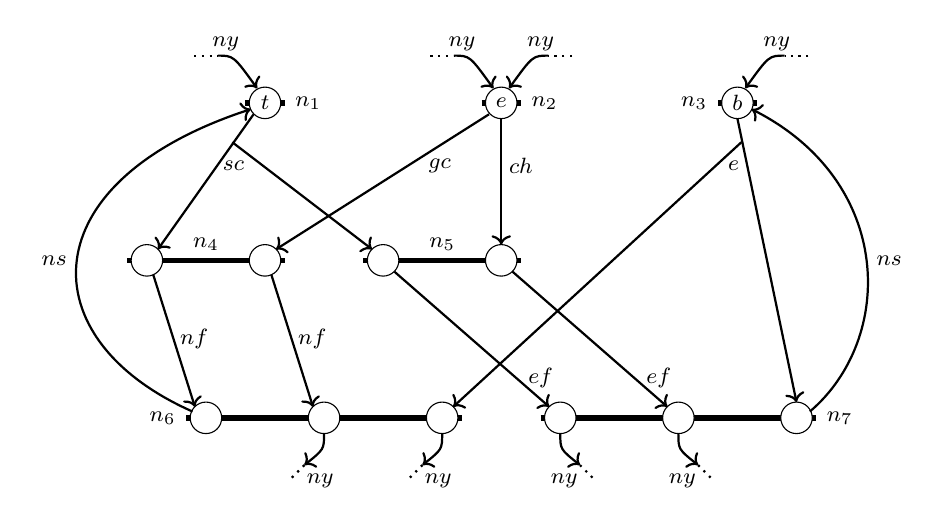
\begin{tikzpicture}[scale=1, every node/.style={transform shape}]

\begin{scope}[line width=2pt]
\draw (-0.25,0) -- (0.25,0);
\draw (2.75,0) -- (3.25,0);
\draw (5.75,0) -- (6.25,0);
\draw (-1.75,-2) -- (0.25,-2);
\draw (1.25,-2) -- (3.25,-2);
\draw (-1,-4) -- (2.5,-4);
\draw (3.5,-4) -- (7,-4);
\end{scope}

\filldraw [fill=white]  (0,0)  circle (2mm) node (t0) {\footnotesize $t$};
\filldraw [fill=white]  (3,0)  circle (2mm) node (e0) {\footnotesize $e$};
\filldraw [fill=white]  (6,0)  circle (2mm) node (b0) {\footnotesize $b$};
\filldraw [fill=white]  (-1.5,-2)  circle (2mm) node (t1) {};
\filldraw [fill=white]  (0,-2)  circle (2mm) node (e1) {};
\filldraw [fill=white]  (1.5,-2)  circle (2mm) node (t2) {};
\filldraw [fill=white]  (3,-2)  circle (2mm) node (e2) {};
\filldraw [fill=white]  (-0.75,-4)  circle (2mm) node (t5) {};
\filldraw [fill=white]  (0.75,-4)  circle (2mm) node (e5) {};
\filldraw [fill=white]  (2.25,-4)  circle (2mm) node (b5) {};
\filldraw [fill=white]  (3.75,-4)  circle (2mm) node (t6) {};
\filldraw [fill=white]  (5.25,-4)  circle (2mm) node (e6) {};
\filldraw [fill=white]  (6.75,-4)  circle (2mm) node (b6) {};

\node at (0.55,0) {\footnotesize $n_1$};
\node at (3.55,0) {\footnotesize $n_2$};
\node at (5.45,0) {\footnotesize $n_3$};
\node at (-0.75,-1.8) {\footnotesize $n_4$};
\node at (2.25,-1.8) {\footnotesize $n_5$};
\node at (-1.3,-4) {\footnotesize $n_6$};
\node at (7.3,-4) {\footnotesize $n_7$};

\node at (-0.4, -0.8) {\footnotesize $sc$};
\node at (2.22, -0.8) {\footnotesize $gc$};
\node at (3.25, -0.8) {\footnotesize $ch$};
\node at (5.95, -0.8) {\footnotesize $e$};
\node at (-0.9,-3) {\footnotesize $nf$};
\node at (0.6, -3) {\footnotesize $nf$};
\node at (3.5,-3.5) {\footnotesize $ef$};
\node at (5,-3.5) {\footnotesize $ef$};
\node at (0.7, -4.8) {\footnotesize $ny$};
\node at (2.2, -4.8) {\footnotesize $ny$};
\node at (3.8, -4.8) {\footnotesize $ny$};
\node at (5.3, -4.8) {\footnotesize $ny$};
\node at (-0.5, 0.75) {\footnotesize $ny$};
\node at (2.5, 0.75) {\footnotesize $ny$};
\node at (3.5, 0.75) {\footnotesize $ny$};
\node at (6.5, 0.75) {\footnotesize $ny$};

\begin{scope}[thick,->]
\draw (-0.145, -0.145) -- (-1.36, -1.86); % t0-t1
\draw (-0.415, -0.5) -- (1.36, -1.86); % t0-t2
\draw (2.845, -0.145) -- (0.14, -1.86); % e0-e1
\draw (3, -0.2) -- (3, -1.8); % e0-e2
\draw (-1.5, -2) + (0.08, -0.18) -- (-0.89, -3.86); % t1-t3
\draw (0, -2) + (0.08, -0.18) -- (0.61, -3.86); % e1-e3
\draw (1.5, -2) + (0.145, -0.145) -- (3.61, -3.86); % t2-t4
\draw (3, -2) + (0.145, -0.145) -- (5.11, -3.86); % e2-e4
\draw (6.05, -0.5) -- (2.39, -3.86); % b0-b3
\draw (6, -0.2) -- (6.75, -3.8); % b0-b4
\draw (-0.92, -3.92) .. controls (-3, -3) and (-3, -1) .. (-0.18, -0.08) node [midway, left] {\footnotesize $ns$}; % t3-t0
\draw (6.92, -3.92) .. controls (8, -3) and (8, -1) .. (6.18, -0.08) node [midway, right] {\footnotesize $ns$}; % b4-b0
\draw (0.75,-4.2) .. controls (0.75, -4.4) .. (0.5,-4.6); % e3-e0
\draw (2.25, -4.2) .. controls (2.25, -4.4) .. (2, -4.6); % b3-b0
\draw (3.75, -4.2) .. controls (3.75, -4.4) .. (4, -4.6); % t4-t0
\draw (5.25, -4.2) .. controls (5.25, -4.4) .. (5.5, -4.6); % e4-e0
\draw (-0.6, 0.6) .. controls (-0.4, 0.6) .. (-0.1, 0.185); % t4-t0
\draw (2.4, 0.6) .. controls (2.6, 0.6) .. (2.9, 0.185); % e3-e0
\draw (3.6, 0.6) .. controls (3.4, 0.6) .. (3.1, 0.185); % e4-e0
\draw (6.6, 0.6) .. controls (6.4, 0.6) .. (6.1, 0.185); % b3-b0
\end{scope}

\begin{scope}[thick, dotted]
\draw (-0.9, 0.6) -- (-0.6, 0.6);
\draw (2.1, 0.6) -- (2.4, 0.6);
\draw (3.9, 0.6) -- (3.6, 0.6);
\draw (6.9, 0.6) -- (6.6, 0.6);
\draw (0.5,-4.6) -- (0.3, -4.8);
\draw (2, -4.6) -- (1.8, -4.8);
\draw (4, -4.6) -- (4.2, -4.8);
\draw (5.5, -4.6) -- (5.7, -4.8);
\end{scope}

\end{tikzpicture}
\caption{The early flowering of many plants due to climate change is creating a critical synchronization problem for insect pollinators like bees \cite{}. When flowers and their necessary pollinators are out of sync, insects lack food, causing potential disruptions throughout the food web. The above figure provides a simplified diagram of this concurrent phenomenon modelled as incomplete distributed negotiations. $t$, $e$, and $b$ are the agents here, denoting \textit{trees}, \textit{environment}, and \textit{bees}, respectively, participating in the nodes $n_1$, $n_2$, and $n_3$, respectively. $n_1$, $n_2$, and $n_3$ are all nodes with a single \textit{domain}, i.e., only one process participates in these nodes. $n_2$ has two outgoing actions, $gc$ and $ch$, denoting \textit{good climate} and \textit{climate change}. $n_1$ and $n_3$ have outgoing actions $sc$ and $e$ respectively, denoting \textit{season change} and \textit{emergence of bees}. In $n_4$, where $t$ and $e$ participate, $nf$ (\textit{normal flowering}) can take place if $gc$ has taken place previously. Otherwise in $n_5$, $ef$ (\textit{early flowering}) takes place if $ch$ was taken in $n_2$ instead of $gc$. $n_6$ and $n_7$ both have single outgoing action $ny$, denoting \textit{next year}, which takes the three processes back to $n_1$, $n_2$, and $n_3$ (four of these arcs are shown partially for the sake of clarity of the picture).}
\label{fig:pollination}
\end{figure}

Figure~\ref{fig:run} shows part of a run of the negotiation in Figure~\ref{fig:pollination}. Gray nodes denote enabled nodes under the current marking.

\begin{figure}[t]
\centering
\begin{minipage}{.49\textwidth}
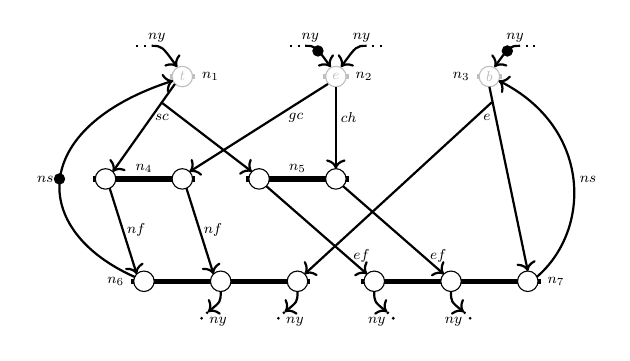
\begin{tikzpicture}[scale=0.65, every node/.style={transform shape}]

\begin{scope}[line width=2pt]
\draw (-1.75,-2) -- (0.25,-2);
\draw (1.25,-2) -- (3.25,-2);
\draw (-1,-4) -- (2.5,-4);
\draw (3.5,-4) -- (7,-4);
\end{scope}

\begin{scope}[line width=2pt, lightgray]
\draw (-0.25,0) -- (0.25,0);
\draw (2.75,0) -- (3.25,0);
\draw (5.75,0) -- (6.25,0);
\end{scope}

\filldraw [lightgray, fill=white]  (0,0)  circle (2mm) node (t0) {\footnotesize $t$};
\filldraw [lightgray, fill=white]  (3,0)  circle (2mm) node (e0) {\footnotesize $e$};
\filldraw [lightgray, fill=white]  (6,0)  circle (2mm) node (b0) {\footnotesize $b$};
\filldraw [fill=white]  (-1.5,-2)  circle (2mm) node (t1) {};
\filldraw [fill=white]  (0,-2)  circle (2mm) node (e1) {};
\filldraw [fill=white]  (1.5,-2)  circle (2mm) node (t2) {};
\filldraw [fill=white]  (3,-2)  circle (2mm) node (e2) {};
\filldraw [fill=white]  (-0.75,-4)  circle (2mm) node (t5) {};
\filldraw [fill=white]  (0.75,-4)  circle (2mm) node (e5) {};
\filldraw [fill=white]  (2.25,-4)  circle (2mm) node (b5) {};
\filldraw [fill=white]  (3.75,-4)  circle (2mm) node (t6) {};
\filldraw [fill=white]  (5.25,-4)  circle (2mm) node (e6) {};
\filldraw [fill=white]  (6.75,-4)  circle (2mm) node (b6) {};

\node at (0.55,0) {\footnotesize $n_1$};
\node at (3.55,0) {\footnotesize$n_2$};
\node at (5.45,0) {\footnotesize $n_3$};
\node at (-0.75,-1.8) {\footnotesize $n_4$};
\node at (2.25,-1.8) {\footnotesize $n_5$};
\node at (-1.3,-4) {\footnotesize $n_6$};
\node at (7.3,-4) {\footnotesize $n_7$};

\node at (-0.4, -0.8) {\footnotesize $sc$};
\node at (2.22, -0.8) {\footnotesize $gc$};
\node at (3.25, -0.8) {\footnotesize $ch$};
\node at (5.95, -0.8) {\footnotesize $e$};
\node at (-0.9,-3) {\footnotesize $nf$};
\node at (0.6, -3) {\footnotesize $nf$};
\node at (3.5,-3.5) {\footnotesize $ef$};
\node at (5,-3.5) {\footnotesize $ef$};
\node at (0.7, -4.8) {\footnotesize $ny$};
\node at (2.2, -4.8) {\footnotesize $ny$};
\node at (3.8, -4.8) {\footnotesize $ny$};
\node at (5.3, -4.8) {\footnotesize $ny$};
\node at (-0.5, 0.75) {\footnotesize $ny$};
\node at (2.5, 0.75) {\footnotesize $ny$};
\node at (3.5, 0.75) {\footnotesize $ny$};
\node at (6.5, 0.75) {\footnotesize $ny$};

\begin{scope}[thick,->]
\draw (-0.145, -0.145) -- (-1.36, -1.86); %t0-t1
\draw (-0.415, -0.5) -- (1.36, -1.86); %t0-t2
\draw (2.845, -0.145) -- (0.14, -1.86); %e0-e1
\draw (3, -0.2) -- (3, -1.8); %e0-e2
\draw (-1.5, -2) + (0.08, -0.18) -- (-0.89, -3.86); %t1-t3
\draw (0, -2) + (0.08, -0.18) -- (0.61, -3.86); %e1-e3
\draw (1.5, -2) + (0.145, -0.145) -- (3.61, -3.86); %t2-t4
\draw (3, -2) + (0.145, -0.145) -- (5.11, -3.86); %e2-e4
\draw (6.05, -0.5) -- (2.39, -3.86); %b0-b3
\draw (6, -0.2) -- (6.75, -3.8); %b0-b4
\draw (-0.92, -3.92) .. controls (-3, -3) and (-3, -1) .. (-0.18, -0.08) node [midway, left] {\footnotesize $ns$}; %t3-t0
\draw (6.92, -3.92) .. controls (8, -3) and (8, -1) .. (6.18, -0.08) node [midway, right] {\footnotesize $ns$}; %b4-b0
\draw (0.75,-4.2) .. controls (0.75, -4.4) .. (0.5,-4.6) ; %e3-e0
\draw (2.25, -4.2) .. controls (2.25, -4.4) .. (2, -4.6); %b3-b0
\draw (3.75, -4.2) .. controls (3.75, -4.4) .. (4, -4.6); %t4-t0
\draw (5.25, -4.2) .. controls (5.25, -4.4) .. (5.5, -4.6); %e4-e0
\draw (-0.6, 0.6) .. controls (-0.4, 0.6) .. (-0.1, 0.185); %t4-t0
\draw (2.4, 0.6) .. controls (2.6, 0.6) .. (2.9, 0.185); %e3-e0
\draw (3.6, 0.6) .. controls (3.4, 0.6) .. (3.1, 0.185); %e4-e0
\draw (6.6, 0.6) .. controls (6.4, 0.6) .. (6.1, 0.185); %b3-b0
\end{scope}

\begin{scope}[thick, dotted]
\draw (-0.9, 0.6) -- (-0.6, 0.6);
\draw (2.1, 0.6) -- (2.4, 0.6);
\draw (3.9, 0.6) -- (3.6, 0.6);
\draw (6.9, 0.6) -- (6.6, 0.6);
\draw (0.5,-4.6) -- (0.3, -4.8);
\draw (2, -4.6) -- (1.8, -4.8);
\draw (4, -4.6) -- (4.2, -4.8);
\draw (5.5, -4.6) -- (5.7, -4.8);
\end{scope}

\filldraw [fill=black]  (-2.4,-2)  circle (1mm);
\filldraw [fill=black]  (2.65,0.5)  circle (1mm);
\filldraw [fill=black]  (6.35,0.5)  circle (1mm);

\end{tikzpicture}
\end{minipage}
\begin{minipage}{.49\textwidth}
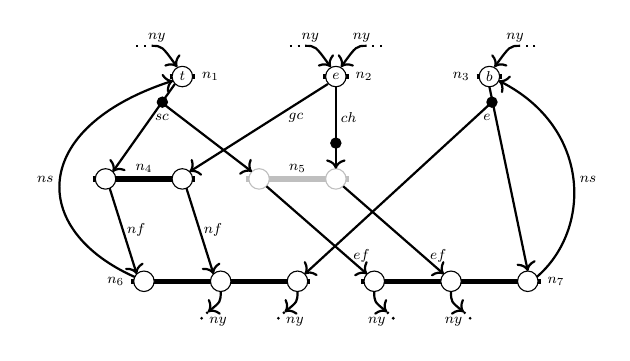
\begin{tikzpicture}[scale=0.65, every node/.style={transform shape}]

\begin{scope}[line width=2pt]
\draw (-0.25,0) -- (0.25,0);
\draw (2.75,0) -- (3.25,0);
\draw (5.75,0) -- (6.25,0);
\draw (-1.75,-2) -- (0.25,-2);
\draw (-1,-4) -- (2.5,-4);
\draw (3.5,-4) -- (7,-4);
\end{scope}

\draw [line width=2pt, lightgray] (1.25,-2) -- (3.25,-2);

\filldraw [fill=white]  (0,0)  circle (2mm) node (t0) {\footnotesize $t$};
\filldraw [fill=white]  (3,0)  circle (2mm) node (e0) {\footnotesize $e$};
\filldraw [fill=white]  (6,0)  circle (2mm) node (b0) {\footnotesize $b$};
\filldraw [fill=white]  (-1.5,-2)  circle (2mm) node (t1) {};
\filldraw [fill=white]  (0,-2)  circle (2mm) node (e1) {};
\filldraw [lightgray, fill=white]  (1.5,-2)  circle (2mm) node (t2) {};
\filldraw [lightgray, fill=white]  (3,-2)  circle (2mm) node (e2) {};
\filldraw [fill=white]  (-0.75,-4)  circle (2mm) node (t5) {};
\filldraw [fill=white]  (0.75,-4)  circle (2mm) node (e5) {};
\filldraw [fill=white]  (2.25,-4)  circle (2mm) node (b5) {};
\filldraw [fill=white]  (3.75,-4)  circle (2mm) node (t6) {};
\filldraw [fill=white]  (5.25,-4)  circle (2mm) node (e6) {};
\filldraw [fill=white]  (6.75,-4)  circle (2mm) node (b6) {};

\node at (0.55,0) {\footnotesize $n_1$};
\node at (3.55,0) {\footnotesize$n_2$};
\node at (5.45,0) {\footnotesize $n_3$};
\node at (-0.75,-1.8) {\footnotesize $n_4$};
\node at (2.25,-1.8) {\footnotesize $n_5$};
\node at (-1.3,-4) {\footnotesize $n_6$};
\node at (7.3,-4) {\footnotesize $n_7$};

\node at (-0.4, -0.8) {\footnotesize $sc$};
\node at (2.22, -0.8) {\footnotesize $gc$};
\node at (3.25, -0.8) {\footnotesize $ch$};
\node at (5.95, -0.8) {\footnotesize $e$};
\node at (-0.9,-3) {\footnotesize $nf$};
\node at (0.6, -3) {\footnotesize $nf$};
\node at (3.5,-3.5) {\footnotesize $ef$};
\node at (5,-3.5) {\footnotesize $ef$};
\node at (0.7, -4.8) {\footnotesize $ny$};
\node at (2.2, -4.8) {\footnotesize $ny$};
\node at (3.8, -4.8) {\footnotesize $ny$};
\node at (5.3, -4.8) {\footnotesize $ny$};
\node at (-0.5, 0.75) {\footnotesize $ny$};
\node at (2.5, 0.75) {\footnotesize $ny$};
\node at (3.5, 0.75) {\footnotesize $ny$};
\node at (6.5, 0.75) {\footnotesize $ny$};

\begin{scope}[thick,->]
\draw (-0.145, -0.145) -- (-1.36, -1.86); %t0-t1
\draw (-0.415, -0.5) -- (1.36, -1.86); %t0-t2
\draw (2.845, -0.145) -- (0.14, -1.86); %e0-e1
\draw (3, -0.2) -- (3, -1.8); %e0-e2
\draw (-1.5, -2) + (0.08, -0.18) -- (-0.89, -3.86); %t1-t3
\draw (0, -2) + (0.08, -0.18) -- (0.61, -3.86); %e1-e3
\draw (1.5, -2) + (0.145, -0.145) -- (3.61, -3.86); %t2-t4
\draw (3, -2) + (0.145, -0.145) -- (5.11, -3.86); %e2-e4
\draw (6.05, -0.5) -- (2.39, -3.86); %b0-b3
\draw (6, -0.2) -- (6.75, -3.8); %b0-b4
\draw (-0.92, -3.92) .. controls (-3, -3) and (-3, -1) .. (-0.18, -0.08) node [midway, left] {\footnotesize $ns$}; %t3-t0
\draw (6.92, -3.92) .. controls (8, -3) and (8, -1) .. (6.18, -0.08) node [midway, right] {\footnotesize $ns$}; %b4-b0
\draw (0.75,-4.2) .. controls (0.75, -4.4) .. (0.5,-4.6) ; %e3-e0
\draw (2.25, -4.2) .. controls (2.25, -4.4) .. (2, -4.6); %b3-b0
\draw (3.75, -4.2) .. controls (3.75, -4.4) .. (4, -4.6); %t4-t0
\draw (5.25, -4.2) .. controls (5.25, -4.4) .. (5.5, -4.6); %e4-e0
\draw (-0.6, 0.6) .. controls (-0.4, 0.6) .. (-0.1, 0.185); %t4-t0
\draw (2.4, 0.6) .. controls (2.6, 0.6) .. (2.9, 0.185); %e3-e0
\draw (3.6, 0.6) .. controls (3.4, 0.6) .. (3.1, 0.185); %e4-e0
\draw (6.6, 0.6) .. controls (6.4, 0.6) .. (6.1, 0.185); %b3-b0
\end{scope}

\begin{scope}[thick, dotted]
\draw (-0.9, 0.6) -- (-0.6, 0.6);
\draw (2.1, 0.6) -- (2.4, 0.6);
\draw (3.9, 0.6) -- (3.6, 0.6);
\draw (6.9, 0.6) -- (6.6, 0.6);
\draw (0.5,-4.6) -- (0.3, -4.8);
\draw (2, -4.6) -- (1.8, -4.8);
\draw (4, -4.6) -- (4.2, -4.8);
\draw (5.5, -4.6) -- (5.7, -4.8);
\end{scope}

\filldraw [fill=black]  (-0.39,-0.5)  circle (1mm);
\filldraw [fill=black]  (3,-1.3)  circle (1mm);
\filldraw [fill=black]  (6.05,-0.5)  circle (1mm);

\end{tikzpicture}
\end{minipage}
\begin{minipage}{.49\textwidth}
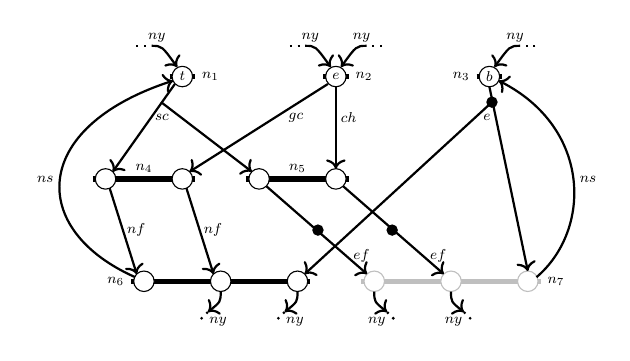
\begin{tikzpicture}[scale=0.65, every node/.style={transform shape}]

\begin{scope}[line width=2pt]
\draw (-0.25,0) -- (0.25,0);
\draw (2.75,0) -- (3.25,0);
\draw (5.75,0) -- (6.25,0);
\draw (-1.75,-2) -- (0.25,-2);
\draw (1.25,-2) -- (3.25,-2);
\draw (-1,-4) -- (2.5,-4);
\end{scope}

\draw [line width=2pt, lightgray] (3.5,-4) -- (7,-4);

\filldraw [fill=white]  (0,0)  circle (2mm) node (t0) {\footnotesize $t$};
\filldraw [fill=white]  (3,0)  circle (2mm) node (e0) {\footnotesize $e$};
\filldraw [fill=white]  (6,0)  circle (2mm) node (b0) {\footnotesize $b$};
\filldraw [fill=white]  (-1.5,-2)  circle (2mm) node (t1) {};
\filldraw [fill=white]  (0,-2)  circle (2mm) node (e1) {};
\filldraw [fill=white]  (1.5,-2)  circle (2mm) node (t2) {};
\filldraw [fill=white]  (3,-2)  circle (2mm) node (e2) {};
\filldraw [fill=white]  (-0.75,-4)  circle (2mm) node (t5) {};
\filldraw [fill=white]  (0.75,-4)  circle (2mm) node (e5) {};
\filldraw [fill=white]  (2.25,-4)  circle (2mm) node (b5) {};
\filldraw [lightgray, fill=white]  (3.75,-4)  circle (2mm) node (t6) {};
\filldraw [lightgray, fill=white]  (5.25,-4)  circle (2mm) node (e6) {};
\filldraw [lightgray, fill=white]  (6.75,-4)  circle (2mm) node (b6) {};

\node at (0.55,0) {\footnotesize $n_1$};
\node at (3.55,0) {\footnotesize$n_2$};
\node at (5.45,0) {\footnotesize $n_3$};
\node at (-0.75,-1.8) {\footnotesize $n_4$};
\node at (2.25,-1.8) {\footnotesize $n_5$};
\node at (-1.3,-4) {\footnotesize $n_6$};
\node at (7.3,-4) {\footnotesize $n_7$};

\node at (-0.4, -0.8) {\footnotesize $sc$};
\node at (2.22, -0.8) {\footnotesize $gc$};
\node at (3.25, -0.8) {\footnotesize $ch$};
\node at (5.95, -0.8) {\footnotesize $e$};
\node at (-0.9,-3) {\footnotesize $nf$};
\node at (0.6, -3) {\footnotesize $nf$};
\node at (3.5,-3.5) {\footnotesize $ef$};
\node at (5,-3.5) {\footnotesize $ef$};
\node at (0.7, -4.8) {\footnotesize $ny$};
\node at (2.2, -4.8) {\footnotesize $ny$};
\node at (3.8, -4.8) {\footnotesize $ny$};
\node at (5.3, -4.8) {\footnotesize $ny$};
\node at (-0.5, 0.75) {\footnotesize $ny$};
\node at (2.5, 0.75) {\footnotesize $ny$};
\node at (3.5, 0.75) {\footnotesize $ny$};
\node at (6.5, 0.75) {\footnotesize $ny$};

\begin{scope}[thick,->]
\draw (-0.145, -0.145) -- (-1.36, -1.86); %t0-t1
\draw (-0.415, -0.5) -- (1.36, -1.86); %t0-t2
\draw (2.845, -0.145) -- (0.14, -1.86); %e0-e1
\draw (3, -0.2) -- (3, -1.8); %e0-e2
\draw (-1.5, -2) + (0.08, -0.18) -- (-0.89, -3.86); %t1-t3
\draw (0, -2) + (0.08, -0.18) -- (0.61, -3.86); %e1-e3
\draw (1.5, -2) + (0.145, -0.145) -- (3.61, -3.86); %t2-t4
\draw (3, -2) + (0.145, -0.145) -- (5.11, -3.86); %e2-e4
\draw (6.05, -0.5) -- (2.39, -3.86); %b0-b3
\draw (6, -0.2) -- (6.75, -3.8); %b0-b4
\draw (-0.92, -3.92) .. controls (-3, -3) and (-3, -1) .. (-0.18, -0.08) node [midway, left] {\footnotesize $ns$}; %t3-t0
\draw (6.92, -3.92) .. controls (8, -3) and (8, -1) .. (6.18, -0.08) node [midway, right] {\footnotesize $ns$}; %b4-b0
\draw (0.75,-4.2) .. controls (0.75, -4.4) .. (0.5,-4.6) ; %e3-e0
\draw (2.25, -4.2) .. controls (2.25, -4.4) .. (2, -4.6); %b3-b0
\draw (3.75, -4.2) .. controls (3.75, -4.4) .. (4, -4.6); %t4-t0
\draw (5.25, -4.2) .. controls (5.25, -4.4) .. (5.5, -4.6); %e4-e0
\draw (-0.6, 0.6) .. controls (-0.4, 0.6) .. (-0.1, 0.185); %t4-t0
\draw (2.4, 0.6) .. controls (2.6, 0.6) .. (2.9, 0.185); %e3-e0
\draw (3.6, 0.6) .. controls (3.4, 0.6) .. (3.1, 0.185); %e4-e0
\draw (6.6, 0.6) .. controls (6.4, 0.6) .. (6.1, 0.185); %b3-b0
\end{scope}

\begin{scope}[thick, dotted]
\draw (-0.9, 0.6) -- (-0.6, 0.6);
\draw (2.1, 0.6) -- (2.4, 0.6);
\draw (3.9, 0.6) -- (3.6, 0.6);
\draw (6.9, 0.6) -- (6.6, 0.6);
\draw (0.5,-4.6) -- (0.3, -4.8);
\draw (2, -4.6) -- (1.8, -4.8);
\draw (4, -4.6) -- (4.2, -4.8);
\draw (5.5, -4.6) -- (5.7, -4.8);
\end{scope}

\filldraw [fill=black]  (2.65,-3)  circle (1mm);
\filldraw [fill=black]  (4.1,-3)  circle (1mm);
\filldraw [fill=black]  (6.05,-0.5)  circle (1mm);

\end{tikzpicture}
\end{minipage}
\begin{minipage}{.49\textwidth}
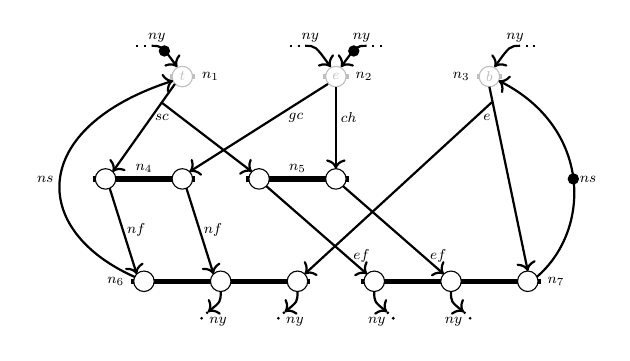
\begin{tikzpicture}[scale=0.65, every node/.style={transform shape}]

\begin{scope}[line width=2pt]
\draw (-1.75,-2) -- (0.25,-2);
\draw (1.25,-2) -- (3.25,-2);
\draw (-1,-4) -- (2.5,-4);
\draw (3.5,-4) -- (7,-4);
\end{scope}

\begin{scope}[line width=2pt, lightgray]
\draw (-0.25,0) -- (0.25,0);
\draw (2.75,0) -- (3.25,0);
\draw (5.75,0) -- (6.25,0);
\end{scope}

\filldraw [lightgray, fill=white]  (0,0)  circle (2mm) node (t0) {\footnotesize $t$};
\filldraw [lightgray, fill=white]  (3,0)  circle (2mm) node (e0) {\footnotesize $e$};
\filldraw [lightgray, fill=white]  (6,0)  circle (2mm) node (b0) {\footnotesize $b$};
\filldraw [fill=white]  (-1.5,-2)  circle (2mm) node (t1) {};
\filldraw [fill=white]  (0,-2)  circle (2mm) node (e1) {};
\filldraw [fill=white]  (1.5,-2)  circle (2mm) node (t2) {};
\filldraw [fill=white]  (3,-2)  circle (2mm) node (e2) {};
\filldraw [fill=white]  (-0.75,-4)  circle (2mm) node (t5) {};
\filldraw [fill=white]  (0.75,-4)  circle (2mm) node (e5) {};
\filldraw [fill=white]  (2.25,-4)  circle (2mm) node (b5) {};
\filldraw [fill=white]  (3.75,-4)  circle (2mm) node (t6) {};
\filldraw [fill=white]  (5.25,-4)  circle (2mm) node (e6) {};
\filldraw [fill=white]  (6.75,-4)  circle (2mm) node (b6) {};

\node at (0.55,0) {\footnotesize $n_1$};
\node at (3.55,0) {\footnotesize$n_2$};
\node at (5.45,0) {\footnotesize $n_3$};
\node at (-0.75,-1.8) {\footnotesize $n_4$};
\node at (2.25,-1.8) {\footnotesize $n_5$};
\node at (-1.3,-4) {\footnotesize $n_6$};
\node at (7.3,-4) {\footnotesize $n_7$};

\node at (-0.4, -0.8) {\footnotesize $sc$};
\node at (2.22, -0.8) {\footnotesize $gc$};
\node at (3.25, -0.8) {\footnotesize $ch$};
\node at (5.95, -0.8) {\footnotesize $e$};
\node at (-0.9,-3) {\footnotesize $nf$};
\node at (0.6, -3) {\footnotesize $nf$};
\node at (3.5,-3.5) {\footnotesize $ef$};
\node at (5,-3.5) {\footnotesize $ef$};
\node at (0.7, -4.8) {\footnotesize $ny$};
\node at (2.2, -4.8) {\footnotesize $ny$};
\node at (3.8, -4.8) {\footnotesize $ny$};
\node at (5.3, -4.8) {\footnotesize $ny$};
\node at (-0.5, 0.75) {\footnotesize $ny$};
\node at (2.5, 0.75) {\footnotesize $ny$};
\node at (3.5, 0.75) {\footnotesize $ny$};
\node at (6.5, 0.75) {\footnotesize $ny$};

\begin{scope}[thick,->]
\draw (-0.145, -0.145) -- (-1.36, -1.86); %t0-t1
\draw (-0.415, -0.5) -- (1.36, -1.86); %t0-t2
\draw (2.845, -0.145) -- (0.14, -1.86); %e0-e1
\draw (3, -0.2) -- (3, -1.8); %e0-e2
\draw (-1.5, -2) + (0.08, -0.18) -- (-0.89, -3.86); %t1-t3
\draw (0, -2) + (0.08, -0.18) -- (0.61, -3.86); %e1-e3
\draw (1.5, -2) + (0.145, -0.145) -- (3.61, -3.86); %t2-t4
\draw (3, -2) + (0.145, -0.145) -- (5.11, -3.86); %e2-e4
\draw (6.05, -0.5) -- (2.39, -3.86); %b0-b3
\draw (6, -0.2) -- (6.75, -3.8); %b0-b4
\draw (-0.92, -3.92) .. controls (-3, -3) and (-3, -1) .. (-0.18, -0.08) node [midway, left] {\footnotesize $ns$}; %t3-t0
\draw (6.92, -3.92) .. controls (8, -3) and (8, -1) .. (6.18, -0.08) node [midway, right] {\footnotesize $ns$}; %b4-b0
\draw (0.75,-4.2) .. controls (0.75, -4.4) .. (0.5,-4.6) ; %e3-e0
\draw (2.25, -4.2) .. controls (2.25, -4.4) .. (2, -4.6); %b3-b0
\draw (3.75, -4.2) .. controls (3.75, -4.4) .. (4, -4.6); %t4-t0
\draw (5.25, -4.2) .. controls (5.25, -4.4) .. (5.5, -4.6); %e4-e0
\draw (-0.6, 0.6) .. controls (-0.4, 0.6) .. (-0.1, 0.185); %t4-t0
\draw (2.4, 0.6) .. controls (2.6, 0.6) .. (2.9, 0.185); %e3-e0
\draw (3.6, 0.6) .. controls (3.4, 0.6) .. (3.1, 0.185); %e4-e0
\draw (6.6, 0.6) .. controls (6.4, 0.6) .. (6.1, 0.185); %b3-b0
\end{scope}

\begin{scope}[thick, dotted]
\draw (-0.9, 0.6) -- (-0.6, 0.6);
\draw (2.1, 0.6) -- (2.4, 0.6);
\draw (3.9, 0.6) -- (3.6, 0.6);
\draw (6.9, 0.6) -- (6.6, 0.6);
\draw (0.5,-4.6) -- (0.3, -4.8);
\draw (2, -4.6) -- (1.8, -4.8);
\draw (4, -4.6) -- (4.2, -4.8);
\draw (5.5, -4.6) -- (5.7, -4.8);
\end{scope}

\filldraw [fill=black]  (-0.35,0.5)  circle (1mm);
\filldraw [fill=black]  (3.35,0.5)  circle (1mm);
\filldraw [fill=black]  (7.64,-2)  circle (1mm);

\end{tikzpicture}
\end{minipage}
\begin{minipage}{.49\textwidth}
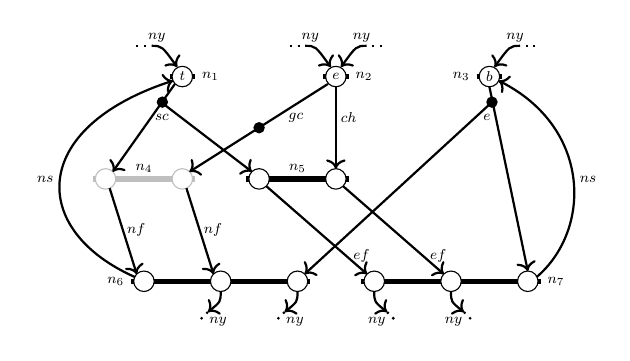
\begin{tikzpicture}[scale=0.65, every node/.style={transform shape}]

\begin{scope}[line width=2pt]
\draw (-0.25,0) -- (0.25,0);
\draw (2.75,0) -- (3.25,0);
\draw (5.75,0) -- (6.25,0);
\draw (1.25,-2) -- (3.25,-2);
\draw (-1,-4) -- (2.5,-4);
\draw (3.5,-4) -- (7,-4);
\end{scope}

\draw [line width=2pt, lightgray] (-1.75,-2) -- (0.25,-2);

\filldraw [fill=white]  (0,0)  circle (2mm) node (t0) {\footnotesize $t$};
\filldraw [fill=white]  (3,0)  circle (2mm) node (e0) {\footnotesize $e$};
\filldraw [fill=white]  (6,0)  circle (2mm) node (b0) {\footnotesize $b$};
\filldraw [lightgray, fill=white]  (-1.5,-2)  circle (2mm) node (t1) {};
\filldraw [lightgray, fill=white]  (0,-2)  circle (2mm) node (e1) {};
\filldraw [fill=white]  (1.5,-2)  circle (2mm) node (t2) {};
\filldraw [fill=white]  (3,-2)  circle (2mm) node (e2) {};
\filldraw [fill=white]  (-0.75,-4)  circle (2mm) node (t5) {};
\filldraw [fill=white]  (0.75,-4)  circle (2mm) node (e5) {};
\filldraw [fill=white]  (2.25,-4)  circle (2mm) node (b5) {};
\filldraw [fill=white]  (3.75,-4)  circle (2mm) node (t6) {};
\filldraw [fill=white]  (5.25,-4)  circle (2mm) node (e6) {};
\filldraw [fill=white]  (6.75,-4)  circle (2mm) node (b6) {};

\node at (0.55,0) {\footnotesize $n_1$};
\node at (3.55,0) {\footnotesize$n_2$};
\node at (5.45,0) {\footnotesize $n_3$};
\node at (-0.75,-1.8) {\footnotesize $n_4$};
\node at (2.25,-1.8) {\footnotesize $n_5$};
\node at (-1.3,-4) {\footnotesize $n_6$};
\node at (7.3,-4) {\footnotesize $n_7$};

\node at (-0.4, -0.8) {\footnotesize $sc$};
\node at (2.22, -0.8) {\footnotesize $gc$};
\node at (3.25, -0.8) {\footnotesize $ch$};
\node at (5.95, -0.8) {\footnotesize $e$};
\node at (-0.9,-3) {\footnotesize $nf$};
\node at (0.6, -3) {\footnotesize $nf$};
\node at (3.5,-3.5) {\footnotesize $ef$};
\node at (5,-3.5) {\footnotesize $ef$};
\node at (0.7, -4.8) {\footnotesize $ny$};
\node at (2.2, -4.8) {\footnotesize $ny$};
\node at (3.8, -4.8) {\footnotesize $ny$};
\node at (5.3, -4.8) {\footnotesize $ny$};
\node at (-0.5, 0.75) {\footnotesize $ny$};
\node at (2.5, 0.75) {\footnotesize $ny$};
\node at (3.5, 0.75) {\footnotesize $ny$};
\node at (6.5, 0.75) {\footnotesize $ny$};

\begin{scope}[thick,->]
\draw (-0.145, -0.145) -- (-1.36, -1.86); %t0-t1
\draw (-0.415, -0.5) -- (1.36, -1.86); %t0-t2
\draw (2.845, -0.145) -- (0.14, -1.86); %e0-e1
\draw (3, -0.2) -- (3, -1.8); %e0-e2
\draw (-1.5, -2) + (0.08, -0.18) -- (-0.89, -3.86); %t1-t3
\draw (0, -2) + (0.08, -0.18) -- (0.61, -3.86); %e1-e3
\draw (1.5, -2) + (0.145, -0.145) -- (3.61, -3.86); %t2-t4
\draw (3, -2) + (0.145, -0.145) -- (5.11, -3.86); %e2-e4
\draw (6.05, -0.5) -- (2.39, -3.86); %b0-b3
\draw (6, -0.2) -- (6.75, -3.8); %b0-b4
\draw (-0.92, -3.92) .. controls (-3, -3) and (-3, -1) .. (-0.18, -0.08) node [midway, left] {\footnotesize $ns$}; %t3-t0
\draw (6.92, -3.92) .. controls (8, -3) and (8, -1) .. (6.18, -0.08) node [midway, right] {\footnotesize $ns$}; %b4-b0
\draw (0.75,-4.2) .. controls (0.75, -4.4) .. (0.5,-4.6) ; %e3-e0
\draw (2.25, -4.2) .. controls (2.25, -4.4) .. (2, -4.6); %b3-b0
\draw (3.75, -4.2) .. controls (3.75, -4.4) .. (4, -4.6); %t4-t0
\draw (5.25, -4.2) .. controls (5.25, -4.4) .. (5.5, -4.6); %e4-e0
\draw (-0.6, 0.6) .. controls (-0.4, 0.6) .. (-0.1, 0.185); %t4-t0
\draw (2.4, 0.6) .. controls (2.6, 0.6) .. (2.9, 0.185); %e3-e0
\draw (3.6, 0.6) .. controls (3.4, 0.6) .. (3.1, 0.185); %e4-e0
\draw (6.6, 0.6) .. controls (6.4, 0.6) .. (6.1, 0.185); %b3-b0
\end{scope}

\begin{scope}[thick, dotted]
\draw (-0.9, 0.6) -- (-0.6, 0.6);
\draw (2.1, 0.6) -- (2.4, 0.6);
\draw (3.9, 0.6) -- (3.6, 0.6);
\draw (6.9, 0.6) -- (6.6, 0.6);
\draw (0.5,-4.6) -- (0.3, -4.8);
\draw (2, -4.6) -- (1.8, -4.8);
\draw (4, -4.6) -- (4.2, -4.8);
\draw (5.5, -4.6) -- (5.7, -4.8);
\end{scope}

\filldraw [fill=black]  (-0.39,-0.5)  circle (1mm);
\filldraw [fill=black]  (1.5,-1)  circle (1mm);
\filldraw [fill=black]  (6.05,-0.5)  circle (1mm);

\end{tikzpicture}
\end{minipage}
\begin{minipage}{.49\textwidth}
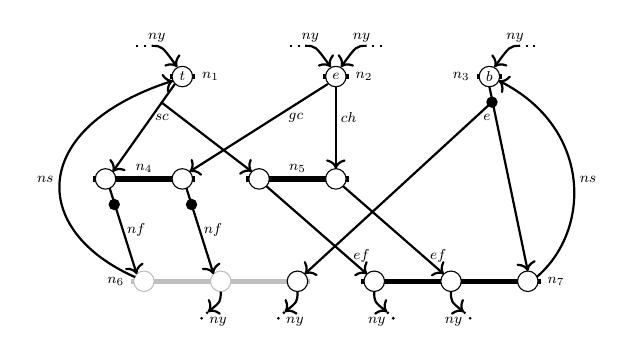
\begin{tikzpicture}[scale=0.65, every node/.style={transform shape}]

\begin{scope}[line width=2pt]
\draw (-0.25,0) -- (0.25,0);
\draw (2.75,0) -- (3.25,0);
\draw (5.75,0) -- (6.25,0);
\draw (-1.75,-2) -- (0.25,-2);
\draw (1.25,-2) -- (3.25,-2);
\draw (3.5,-4) -- (7,-4);
\end{scope}

\draw [line width=2pt, lightgray] (-1,-4) -- (2.5,-4);

\filldraw [fill=white]  (0,0)  circle (2mm) node (t0) {\footnotesize $t$};
\filldraw [fill=white]  (3,0)  circle (2mm) node (e0) {\footnotesize $e$};
\filldraw [fill=white]  (6,0)  circle (2mm) node (b0) {\footnotesize $b$};
\filldraw [fill=white]  (-1.5,-2)  circle (2mm) node (t1) {};
\filldraw [fill=white]  (0,-2)  circle (2mm) node (e1) {};
\filldraw [fill=white]  (1.5,-2)  circle (2mm) node (t2) {};
\filldraw [fill=white]  (3,-2)  circle (2mm) node (e2) {};
\filldraw [lightgray, fill=white]  (-0.75,-4)  circle (2mm) node (t5) {};
\filldraw [lightgray, fill=white]  (0.75,-4)  circle (2mm) node (e5) {};
\filldraw [fill=white]  (2.25,-4)  circle (2mm) node (b5) {};
\filldraw [fill=white]  (3.75,-4)  circle (2mm) node (t6) {};
\filldraw [fill=white]  (5.25,-4)  circle (2mm) node (e6) {};
\filldraw [fill=white]  (6.75,-4)  circle (2mm) node (b6) {};

\node at (0.55,0) {\footnotesize $n_1$};
\node at (3.55,0) {\footnotesize$n_2$};
\node at (5.45,0) {\footnotesize $n_3$};
\node at (-0.75,-1.8) {\footnotesize $n_4$};
\node at (2.25,-1.8) {\footnotesize $n_5$};
\node at (-1.3,-4) {\footnotesize $n_6$};
\node at (7.3,-4) {\footnotesize $n_7$};

\node at (-0.4, -0.8) {\footnotesize $sc$};
\node at (2.22, -0.8) {\footnotesize $gc$};
\node at (3.25, -0.8) {\footnotesize $ch$};
\node at (5.95, -0.8) {\footnotesize $e$};
\node at (-0.9,-3) {\footnotesize $nf$};
\node at (0.6, -3) {\footnotesize $nf$};
\node at (3.5,-3.5) {\footnotesize $ef$};
\node at (5,-3.5) {\footnotesize $ef$};
\node at (0.7, -4.8) {\footnotesize $ny$};
\node at (2.2, -4.8) {\footnotesize $ny$};
\node at (3.8, -4.8) {\footnotesize $ny$};
\node at (5.3, -4.8) {\footnotesize $ny$};
\node at (-0.5, 0.75) {\footnotesize $ny$};
\node at (2.5, 0.75) {\footnotesize $ny$};
\node at (3.5, 0.75) {\footnotesize $ny$};
\node at (6.5, 0.75) {\footnotesize $ny$};

\begin{scope}[thick,->]
\draw (-0.145, -0.145) -- (-1.36, -1.86); %t0-t1
\draw (-0.415, -0.5) -- (1.36, -1.86); %t0-t2
\draw (2.845, -0.145) -- (0.14, -1.86); %e0-e1
\draw (3, -0.2) -- (3, -1.8); %e0-e2
\draw (-1.5, -2) + (0.08, -0.18) -- (-0.89, -3.86); %t1-t3
\draw (0, -2) + (0.08, -0.18) -- (0.61, -3.86); %e1-e3
\draw (1.5, -2) + (0.145, -0.145) -- (3.61, -3.86); %t2-t4
\draw (3, -2) + (0.145, -0.145) -- (5.11, -3.86); %e2-e4
\draw (6.05, -0.5) -- (2.39, -3.86); %b0-b3
\draw (6, -0.2) -- (6.75, -3.8); %b0-b4
\draw (-0.92, -3.92) .. controls (-3, -3) and (-3, -1) .. (-0.18, -0.08) node [midway, left] {\footnotesize $ns$}; %t3-t0
\draw (6.92, -3.92) .. controls (8, -3) and (8, -1) .. (6.18, -0.08) node [midway, right] {\footnotesize $ns$}; %b4-b0
\draw (0.75,-4.2) .. controls (0.75, -4.4) .. (0.5,-4.6) ; %e3-e0
\draw (2.25, -4.2) .. controls (2.25, -4.4) .. (2, -4.6); %b3-b0
\draw (3.75, -4.2) .. controls (3.75, -4.4) .. (4, -4.6); %t4-t0
\draw (5.25, -4.2) .. controls (5.25, -4.4) .. (5.5, -4.6); %e4-e0
\draw (-0.6, 0.6) .. controls (-0.4, 0.6) .. (-0.1, 0.185); %t4-t0
\draw (2.4, 0.6) .. controls (2.6, 0.6) .. (2.9, 0.185); %e3-e0
\draw (3.6, 0.6) .. controls (3.4, 0.6) .. (3.1, 0.185); %e4-e0
\draw (6.6, 0.6) .. controls (6.4, 0.6) .. (6.1, 0.185); %b3-b0
\end{scope}

\begin{scope}[thick, dotted]
\draw (-0.9, 0.6) -- (-0.6, 0.6);
\draw (2.1, 0.6) -- (2.4, 0.6);
\draw (3.9, 0.6) -- (3.6, 0.6);
\draw (6.9, 0.6) -- (6.6, 0.6);
\draw (0.5,-4.6) -- (0.3, -4.8);
\draw (2, -4.6) -- (1.8, -4.8);
\draw (4, -4.6) -- (4.2, -4.8);
\draw (5.5, -4.6) -- (5.7, -4.8);
\end{scope}

\filldraw [fill=black]  (-1.33,-2.5)  circle (1mm);
\filldraw [fill=black]  (0.18,-2.5)  circle (1mm);
\filldraw [fill=black]  (6.05,-0.5)  circle (1mm);

\end{tikzpicture}
\end{minipage}
\caption{A possible run of the negotiation in Figure~\ref{fig:pollination}. Tokens represent the current readiness of each process. Gray nodes denote enabled nodes. The run illustrates how choices at \(n_1\), \(n_2\), and \(n_3\) propagate to subsequent flowering and synchronization behaviour.}
\label{fig:run}
\end{figure}

\smallskip
As in other state-based models, one can define the \emph{reachability graph} of a negotiation: its vertices are all markings reachable from the initial marking \(x_0\), and there is an edge from \(x\) to \(x'\) labelled \((n,r)\) whenever \(x \xrightarrow{(n,r)} x'\). Figure~\ref{fig:rg-pol} depicts part of the reachability graph corresponding to the negotiation fragment in Figure~\ref{fig:pollination}.

\begin{figure}[t]
\centering
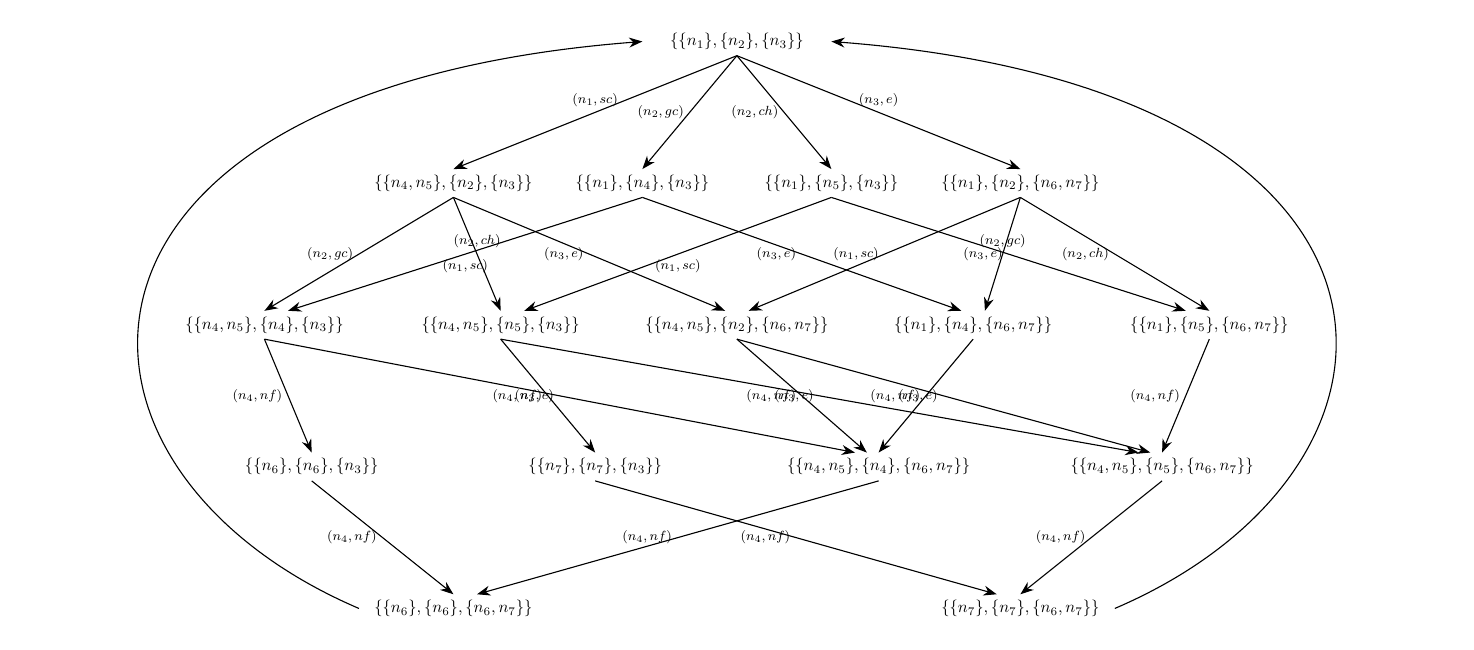
\begin{tikzpicture}[scale=0.6, every node/.style={transform shape}]

\node at (0,0) {$\{\{n_1\}, \{n_2\}, \{n_3\}\}$};
\node at (-6,-3) {$\{\{n_4, n_5\}, \{n_2\}, \{n_3\}\}$};
\node at (-2,-3) {$\{\{n_1\}, \{n_4\}, \{n_3\}\}$};
\node at (2,-3) {$\{\{n_1\}, \{n_5\}, \{n_3\}\}$};
\node at (6,-3) {$\{\{n_1\}, \{n_2\}, \{n_6, n_7\}\}$};
\node at (-10,-6) {$\{\{n_4, n_5\}, \{n_4\}, \{n_3\}\}$};
\node at (-5,-6) {$\{\{n_4, n_5\}, \{n_5\}, \{n_3\}\}$};
\node at (0,-6) {$\{\{n_4, n_5\}, \{n_2\}, \{n_6, n_7\}\}$};
\node at (5,-6) {$\{\{n_1\}, \{n_4\}, \{n_6, n_7\}\}$};
\node at (10,-6) {$\{\{n_1\}, \{n_5\}, \{n_6, n_7\}\}$};
\node at (-9,-9) {$\{\{n_6\}, \{n_6\}, \{n_3\}\}$};
\node at (3,-9) {$\{\{n_4, n_5\}, \{n_4\}, \{n_6, n_7\}\}$};
\node at (-3,-9) {$\{\{n_7\}, \{n_7\}, \{n_3\}\}$};
\node at (9,-9) {$\{\{n_4, n_5\}, \{n_5\}, \{n_6, n_7\}\}$};
\node at (-6,-12) {$\{\{n_6\}, \{n_6\}, \{n_6, n_7\}\}$};
\node at (6,-12) {$\{\{n_7\}, \{n_7\}, \{n_6, n_7\}\}$};

\begin{scope}[-Stealth]
\draw (0,-0.3) -- (-6,-2.7) node [midway, left, above] {\footnotesize $(n_1, sc)$};
\draw (0,-0.3) -- (-2,-2.7) node [midway, left] {\footnotesize $(n_2, gc)$};
\draw (0,-0.3) -- (2,-2.7) node [midway, left] {\footnotesize $(n_2, ch)$};
\draw (0,-0.3) -- (6,-2.7) node [midway, right, above] {\footnotesize $(n_3, e)$};
\draw (-6,-3.3) -- (-10,-5.7) node [midway, left] {\footnotesize $(n_2, gc)$};
\draw (-6,-3.3) -- (-5,-5.7) node [midway, left, above] {\footnotesize $(n_2, ch)$};%
\draw (-6,-3.3) -- (-0.25,-5.7) node [midway, left] {\footnotesize $(n_3, e)$};
\draw (-2,-3.3) -- (-9.5,-5.7) node [midway, left, below] {\footnotesize $(n_1, sc)$};%
\draw (-2,-3.3) -- (4.75,-5.7) node [midway, left] {\footnotesize $(n_3, e)$};
\draw (2,-3.3) -- (-4.5,-5.7) node [midway, left, below] {\footnotesize $(n_1, sc)$};%
\draw (2,-3.3) -- (9.5,-5.7) node [midway, left] {\footnotesize $(n_3, e)$};
\draw (6,-3.3) -- (0.25,-5.7) node [midway, left] {\footnotesize $(n_1, sc)$};
\draw (6,-3.3) -- (5.25,-5.7) node [midway, left, above] {\footnotesize $(n_2, gc)$};%
\draw (6,-3.3) -- (10,-5.7) node [midway, left] {\footnotesize $(n_2, ch)$};
\draw (-10,-6.3) -- (-9,-8.7) node [midway, left] {\footnotesize $(n_4, nf)$};
\draw (-10,-6.3) -- (2.5,-8.7) node [midway, left] {\footnotesize $(n_3, e)$};
\draw (-5,-6.3) -- (-3,-8.7) node [midway, left] {\footnotesize $(n_4, nf)$};
\draw (-5,-6.3) -- (8.5,-8.7) node [midway, left] {\footnotesize $(n_3, e)$};
\draw (0,-6.3) -- (2.75,-8.7) node [midway, left] {\footnotesize $(n_4, nf)$};
\draw (0,-6.3) -- (8.75,-8.7) node [midway, left] {\footnotesize $(n_3, e)$};
\draw (5,-6.3) -- (3,-8.7) node [midway, left] {\footnotesize $(n_4, nf)$};
\draw (10,-6.3) -- (9,-8.7) node [midway, left] {\footnotesize $(n_4, nf)$};
\draw (-9,-9.3) -- (-6,-11.7) node [midway, left] {\footnotesize $(n_4, nf)$};
\draw (-3,-9.3) -- (5.5,-11.7) node [midway, left] {\footnotesize $(n_4, nf)$};
\draw (3,-9.3) -- (-5.5,-11.7) node [midway, left] {\footnotesize $(n_4, nf)$};
\draw (9,-9.3) -- (6,-11.7) node [midway, left] {\footnotesize $(n_4, nf)$};
\draw (-8, -12) .. controls (-15, -9) and (-15, -1) .. (-2, 0);
\draw (8, -12) .. controls (15, -9) and (15, -1) .. (2, 0);
\end{scope}

\end{tikzpicture}
\caption{Part of the reachability graph for the negotiation in Figure~\ref{fig:pollination}. Each vertex is a marking (represented symbolically), and edges are labelled by occurring outcomes \((n,r)\). The number of reachable markings can grow exponentially in the number of nodes due to hyperarc branching.}
\label{fig:rg-pol}
\end{figure}

In general, occurrence sequences can be arbitrarily long, and the number of reachable markings can be very large. For negotiations with multiple hyperarcs, each with branching degree \(n\), the number of distinct branching patterns can grow as \(n^k\), where \(k\) is the number of hyperarcs, leading to an exponential blow-up in the marking graph. It is known that the reachability problem for negotiations is PSPACE-complete in general, and already coNP-hard and in DP for acyclic negotiations (see, e.g.,~\cite{EsparzaDeselNegotiations}).

\paragraph{Key observations from this example.}
This example illustrates several features of negotiations:
\begin{enumerate}
\item \textbf{Multiparty interactions are atomic:} An interaction involves all its participating agents simultaneously and cannot be decomposed into pairwise steps. Node \(n_6\) requires all three processes to participate simultaneously.
\item \textbf{Synchronization is explicit, not emergent:} Agents synchronize because the model says so, not because of shared state.
\item \textbf{Independence is visible in the structure:} Disjoint sets of agents can proceed independently, and this is evident in the graph itself. Nodes \(n_1\), \(n_2\) and \(n_3\) can occur in either order, or even conceptually ``at the same time'' since they involve disjoint sets of processes.
\item \textbf{Non-determinism:} After \(n_1\), \(t\) is ready to engage in both \(n_4\) and \(n_5\) and the choice is resolved only through interaction.
\item \textbf{Control flow is global, not agent-local:} Choices made at one node propagate to future possibilities for all involved agents.
\item \textbf{Information transfer:} The example highlights that synchronization itself acts as a mechanism for
information flow between agents -- by participating in a joint interaction, agents
implicitly exchange information that influences future behavior, even though no
explicit shared state or data is modeled.
\item \textbf{Succicntness:} The underlying reachability graph could be exponential on the number of nodes.
\end{enumerate}

Negotiations have been applied to the analysis of business processes, often modelled by workflow Petri nets~\cite{EsparzaWorkflow}. Such nets underlie popular graphical notations like BPMN, EPC, and UML Activity Diagrams~\cite{DijkmanBPMN}. Deterministic negotiations are closely related to free-choice workflow nets~\cite{EsparzaFreeChoice}, which are expressive enough for many industrial processes; empirical studies show that a large fraction of real-world models fall into the free-choice class.

In the remainder of the thesis, we extend negotiations with quantitative timing information, in the form of local clocks and time constraints, and study reachability in this enriched model.

%_____________________________________________________________________________

\section{Local-Timed Negotiations}

This thesis studies \emph{local-timed negotiations} (LTNs)~\cite{LTNOriginal}, which combine the multiparty synchronization structure of negotiations with quantitative timing constraints inspired by timed automata.

\subsection{Key Ideas}

Each agent in an LTN maintains its own \emph{local reference time}, evolving independently. Like timed automata, each agent has a set of \emph{local clocks} measuring elapsed time. Outcomes can be annotated with:
\begin{itemize}
\item \textbf{Guards}: Constraints on local clocks (e.g., $x \geq 5$, $y < 10$)
\item \textbf{Resets}: Clocks to reset to zero when the outcome occurs
\end{itemize}

The crucial new feature is \emph{explicit time synchronization}. Some interactions may \emph{synchronize} the local reference times of participating agents, aligning their clocks. Other interactions leave local times independent. This creates a spectrum between fully asynchronous systems (no synchronization) and tightly coupled systems (frequent synchronization).

\paragraph{Why Local Time?} The local-time approach offers several advantages:
\begin{enumerate}
\item \textbf{Explicit independence}: When two nodes involve disjoint agent sets and neither synchronizes time, they are genuinely independent and can be reordered freely.
\item \textbf{Realistic modeling}: In distributed systems, components often have their own clocks (e.g., different computers, different sensors). Local time reflects this reality.
\item \textbf{Partial-order potential}: Explicit independence enables partial-order reduction techniques, potentially avoiding exploration of redundant interleavings.
\item \textbf{Flexible synchronization}: The model supports both tightly synchronized systems (e.g., real-time embedded systems with global clock) and loosely coupled systems (e.g., distributed protocols with occasional synchronization).
\end{enumerate}

\paragraph{Why not assume global time?}
A natural question is why we do not assume a single global time shared by all
agents, as is standard in timed automata and their networks. Under such a
global-time semantics, timed negotiations collapse to a classical timed automaton
obtained as the synchronous product of the agents’ local timed behaviors: all
clocks advance uniformly, interactions implicitly synchronize time, and
reachability reduces to standard timed-automata reachability analyzable via region
or zone-based techniques.

This global-time assumption fundamentally alters the concurrency model. Independent
agents can no longer progress at different rates, and relative delays between
agents do not persist across interactions. As a result, the semantics collapses
from an interaction-centric concurrent model to an interleaving-based model with
global temporal coordination.

Local-timed negotiations deliberately reject this assumption. By allowing agents
to maintain independent reference times, the model preserves structural
independence and makes temporal coordination explicit. This semantic freedom is
essential for the expressiveness of the model and for isolating the boundary
between decidability and undecidability explored in this thesis.

\subsection{The Challenge of Mixed Synchronization}

Allowing arbitrary mixtures of time-synchronizing and non-synchronizing interactions creates a powerful but complex model. The interplay between independent local clocks and selective synchronization can simulate sophisticated computational behaviors. As we will show, this generality comes at a cost: reachability becomes undecidable.

However, by imposing restrictions on synchronization patterns, clock usage, or behavioral properties, we can recover decidability. Understanding which restrictions suffice—and which do not—is the central technical challenge of this thesis.
%_____________________________________________________________________________

\section{Contributions}

This thesis provides the first systematic study of decidability and complexity for reachability in local-timed negotiations. Our main contributions are:

\subsection{Undecidability of General LTNs}

We prove that reachability is \emph{undecidable} for LTNs that permit arbitrary mixtures of time-synchronizing and non-synchronizing interactions. The proof uses a reduction from the halting problem for two-counter machines, showing that LTNs with mixed synchronization can encode unbounded computation. This establishes a sharp boundary: full generality leads to undecidability.

\subsection{Two PSPACE-Complete Structural Fragments}

We identify two extreme fragments where reachability is decidable and PSPACE-complete:

\paragraph{Synchronization-free LTNs.} When \emph{no} interactions synchronize local times, agents evolve completely independently. We show that reachability remains PSPACE-complete. The proof constructs a suitable region abstraction that accounts for local timing constraints without global coordination.

\paragraph{Fully-synchronizing LTNs.} When \emph{all} interactions synchronize local times, the system behaves like a classical timed automaton with global time. We again obtain PSPACE-completeness, connecting to known complexity results for timed automata.

These results delineate the extremes of the synchronization spectrum and provide baseline complexity bounds.

\subsection{Decidability via Drift-Boundedness}

We introduce a semantic restriction called \emph{drift-boundedness}. An LTN is drift-bounded by constant $K$ if in every behavior, the difference between local times of any two agents (the \emph{drift}) never exceeds $K$. Intuitively, even though agents have independent clocks, their times cannot diverge too far.

We prove that reachability is \emph{decidable} for drift-bounded LTNs. The key insight is to construct a region automaton over the untimed marking graph, where regions bound not only clock values but also inter-agent time differences. Drift-boundedness ensures this abstraction is finite and sound.

Drift-boundedness is inspired by similar notions for networks of timed automata~\cite{DriftTA1,DriftTA2}. Our contribution is adapting this concept to the negotiation setting and proving decidability.

\subsection{Decidability via Connected Communication}

We define a syntactic fragment called \emph{connectedly-communicating LTNs}. Informally, an LTN is connectedly-communicating if in every cycle of the marking graph, each agent synchronizes (directly or indirectly) with every other agent through time-synchronizing interactions.

We formalize this using \emph{communication graphs} associated with loops in the marking graph. A loop is connectedly-communicating if its communication graph is connected. We prove that if \emph{all} loops are connectedly-communicating, then reachability is decidable.

The intuition is that frequent synchronization prevents unbounded drift and limits the computational power of the system. This fragment is inspired by restrictions in hierarchical message sequence charts~\cite{HenriksenMSG} and distributed controller synthesis~\cite{PnueliRosner}, adapted to our negotiation-based setting.

\subsection{Summary of Landscape}

Our results provide a comprehensive picture of decidability for LTN reachability:

\begin{center}
\begin{tabular}{lcc}
\toprule
\textbf{Fragment} & \textbf{Reachability} \\
\midrule
General LTNs (mixed synchronization) & Undecidable \\
Synchronization-free LTNs & Decidable \\
Fully-synchronizing LTNs & Decidable \\
Drift-bounded LTNs & Decidable \\
Connectedly-communicating LTNs & Decidable \\
\bottomrule
\end{tabular}
\end{center}

%_____________________________________________________________________________

\section{Organization of the thesis}
\label{sec:organization}

The thesis is structured in two main parts.

\medskip
\noindent\textbf{Part~I: Modelling local-timed negotiations and undecidability.}

\begin{itemize}
  \item \textbf{Chapter~\ref{chap:preliminaries}} introduces the basic notions and notations used throughout the thesis. We recall the definitions of negotiations, timed automata, and networks of timed automata, accompanied by illustrative examples.
  \item \textbf{Chapter~\ref{chap:ltn}} defines local-timed negotiations formally. We develop their semantics, introduce local clocks and time-synchronizing interactions, and show that reachability is undecidable in the general LTN model.
\end{itemize}

\medskip
\noindent\textbf{Part~II: Decidable subclasses of local-timed negotiations.}

\begin{itemize}
  \item \textbf{Chapter~\ref{chap:synch-fragments}} studies two extreme structural fragments of LTNs: synchronization-free negotiations and always-synchronizing negotiations. We prove that reachability is PSPACE-complete in both cases.
  \item \textbf{Chapter~\ref{chap:drift-bounded}} introduces drift-bounded LTNs. We formalize drift-boundedness, study its algorithmic properties, and show that reachability is decidable in this fragment via a region-based construction over untimed behaviours.
  \item \textbf{Chapter~\ref{chap:connected-communicating}} presents the fragment of connectedly-communicating LTNs. We formalize the associated communication graphs, prove decidability of reachability, and discuss potential extensions to weaker communication assumptions.
\end{itemize}

\medskip
Each chapter concludes with a section of \emph{concluding remarks}, summarizing the main definitions and results and providing pointers to later chapters where they are used.

\paragraph{Conceptual takeaway.}
The results developed in this thesis can be understood as exploring a design space
organized along three independent axes. 

\begin{enumerate}
\item The first axis is \emph{temporal coupling}: whether agents evolve with respect to a single global time or maintain independent local reference times. 
\item The second axis is \emph{synchronization strength}, ranging from no synchronization, through selective synchronization at chosen interactions, to mandatory synchronization at every interaction. 
\item The third axis is the \emph{persistence of timing information}: whether relative timing differences between agents can accumulate and persist across interactions or are periodically eliminated by synchronization.
\end{enumerate}
Local-timed negotiations inhabit the region of this space where
time is local, synchronization is explicit and optional, and relative timing
information can persist. The remainder of the thesis shows how different restrictions
along these axes delineate the precise boundary between decidability and
undecidability of reachability.
%_____________________________________________________________________________

\section{Related work}
\label{sec:related}

We briefly survey work related to local-time semantics, timed models of concurrency, negotiation models, and decidable fragments in distributed systems.

\paragraph{Local-time semantics and timed automata.}
A local-time semantics was proposed for networks of timed automata in~\cite{LocalTimeTA}. Recently, this semantics has been used for zone-based verification of reachability properties~\cite{LocalZone1,LocalZone2} and B\"uchi reachability~\cite{LocalBuchi}. Local-time semantics has also been investigated as a foundation for applying partial-order methods to timed automata. In networks of timed automata, independence between actions becomes more explicit under local-time semantics, leading to zone graphs that contain ``diamonds'' corresponding to commuting actions, which can mitigate the combinatorial explosion due to interleavings.

In contrast, our work starts from local-time semantics as a primitive feature, and makes synchronization an explicit option at the level of the negotiation model. This emphasises independence and true concurrency in the presence of time.

\paragraph{Timed models mixing concurrency and timing.}
A variety of models extend classical concurrency formalisms with timing information, including time Petri nets~\cite{MerlinTimePN}, timed-arc Petri nets~\cite{HansenTimedArc}, and time-constrained message sequence charts~\cite{AlurMSC}. Each provides a different balance between expressiveness and tractability. Partial-order semantics for such models have also been explored, for example via unfoldings and finite complete prefixes~\cite{EsparzaUnfoldings,KhomenkoTimePN}.

To the best of our knowledge, real-time extensions of negotiations have not been systematically studied before the introduction of local-timed negotiations in~\cite{LTNOriginal}.

\paragraph{Negotiations and concurrency theory.}
Negotiations were introduced in~\cite{EsparzaDeselNegotiations} as a primitive model of concurrency rooted in atomic multiparty interactions. They have been related to workflow Petri nets and business process models~\cite{EsparzaWorkflow,EsparzaFreeChoice}, and studied in terms of soundness, summarization, and complexity. The notion of atomic negotiations and occurrence sequences provides a natural setting for partial-order reasoning.

\paragraph{Bounded drift and partial-order methods.}
The idea of bounding the drift between local times of processes has been studied for networks of timed automata in~\cite{DriftTA1,DriftTA2}. In that setting, drift-boundedness is used to design simulation techniques and to ensure the finiteness of certain abstractions in zone-based verification. Our drift-boundedness notion for LTNs is analogous in spirit, but tailored to the negotiation model and its marking-based semantics.

Partial-order semantics for timed systems, including time Petri nets and timed automata, have been investigated in~\cite{EsparzaUnfoldings,KhomenkoTimePN,LocalBuchi}. These works show that combining timing with partial orders can retain enough structure for efficient verification. Our work aims at a similar goal in the context of negotiations.

\paragraph{Connected communication and decidable fragments.}
The connectedly-communicating fragment of LTNs is inspired by the The MSO theory of connectedly communicating processes~\cite{}. Similar restrictions has been studied in hierarchical message sequence charts~\cite{HenriksenMSG}, where communication structure enforces decidability of the emptiness problem. It is also related to connectedly-communicating architectures in distributed controller synthesis~\cite{PnueliRosner}, where certain connectivity assumptions restore decidability. While the technical settings differ, the underlying theme is that suitable communication constraints can balance expressiveness and decidability.

Local-timed negotiations were first introduced in~\cite{}, where it was shown that reachability is decidable in two special cases: when all nodes are time-synchronizing (fully synchronizing fragment), or when none are (synchronization-free fragment). Our work extends and systematizes these results, and complements them with drift-bounded and connectedly-communicating fragments.

%Finally, throughout the thesis we highlight connections to partial-order verification, unfoldings, and true concurrency models. These connections suggest directions for future work, such as combining our negotiation-based framework with advanced POR techniques developed for timed and untimed models.

%_____________________________________________________________________________


\part{Adding local time constraints to negotiations}
%_________________________________________________________________________________________

\chapter{Preliminaries}
\label{chap:preliminaries}

This chapter introduces the formal models and core definitions used throughout the thesis. We present \emph{negotiations} as our framework for modeling concurrency, and \emph{timed automata} as our reference model for quantitative time. Both models serve as building blocks for local-timed negotiations, which we introduce in Chapter~\ref{chap:ltn}.

All definitions presented here are standard or adapted from existing literature, particularly~\cite{EsparzaDeselNegotiations,AlurDillTA}. This chapter is purely foundational—no new results appear. The level of detail ensures that later constructions can be understood without consulting original sources.

\paragraph{Organization.} Section~\ref{sec:negotiations} introduces negotiations, their semantics, and key examples. Section~\ref{sec:timed-automata} recalls timed automata, region abstractions, and their decidability results. Section~\ref{sec:networks-ta} briefly covers networks of timed automata. Section~\ref{sec:summary} summarizes and previews the synthesis of these models in local-timed negotiations.

%_________________________________________________________________________________________

\section{Negotiations}
Negotiations provide an interaction-centric model of concurrency in which synchronization is explicit and causality is transparent; this makes them a natural substrate for studying the impact of timing and synchronization on reachability.

The formal model of distributed negotiations is inspired by van der Aalst’s workflow Petri nets~\cite{}. A negotiation consists of a collection of \emph{atomic negotiations} (also called atoms or nodes), each representing a synchronized interaction among a non-empty set of agents (also called processes). Each atom has a finite set of possible \emph{outcomes}, corresponding to the different ways in which the interaction may resolve.

Atoms are composed into a distributed negotiation by means of a \emph{next-atoms} function that determines, for each atom, each participating agent, and each outcome, the set of atoms that the agent is ready to engage in next if that outcome occurs. We assume that every negotiation has a distinguished initial atom involving all agents, which marks the start of the interaction.

In the original definition, outcomes are additionally equipped with state-transformers that update internal states of the participating agents. These internal states do not influence which atoms are enabled, and will be abstracted away later in this chapter, as we focus exclusively on the control-flow behaviour of negotiations.

Negotiations are particularly well-suited for modelling distributed workflows, business processes, and coordination protocols, and reveals structural properties that are not easily visible in state-based models. In particular, negotiations make synchronization explicit at the level of interactions, rather than encoding it indirectly via shared places or states, which leads to different structural and algorithmic properties.

%---------------------------------------------------------------------------------------------------------------------------------------------

\subsection{Syntax and Semantics}

We present negotiations in a control-flow-oriented form that abstracts away internal agent states. This abstraction suffices for reachability analysis, since internal states do not influence the enablement or ordering of atoms. The simplified model will later be extended with timing constraints in Chapter~\ref{chap:ltn}. Its relationship to the standard definition with transformers and internal states is discussed in Section~\ref{sec:standard-def}.

This is not a new model, but an abstraction of the standard one that preserves exactly the control-flow behaviour relevant for reachability.

\begin{definition}[Negotiation]
\label{def:negotiation}
Let $P$ be a finite set of \emph{agents} (or \emph{processes}), and $\S$ a finite set of \emph{outcomes}. A \textsf{negotiation} $\mathcal{N}$ is a tuple $(N, \text{dom}, \delta)$ where:
\begin{itemize}
\item $N$ is a finite set of \emph{nodes} (also called \emph{atoms} or \emph{atomic negotiations}),
\item $\text{dom} : N \rightarrow 2^P \setminus \{\emptyset\}$ maps each node to a non-empty subset of agents called its \emph{domain}; we assume $\text{dom}(n_{\text{in}}) = P$ for a distinguished \emph{initial node} $n_{\text{in}}$,
\item $\delta = \{\delta_p\}_{p \in P}$ is a tuple of transition relations, one per agent, where $\delta_p : N_p \times \S \rightarrow 2^{N_p}$ with $N_p = \{n \in N \mid p \in \text{dom}(n)\}$. For a node $n$ with outcome $r$, the set $\delta_p(n,r)$ specifies which nodes agent $p$ becomes ready for next if outcome $r$ occurs.
\end{itemize}
We call pairs $(n,r)$ with $n \in N$ and $r$ an outcome associated with $n$ the \emph{locations} of the negotiation.
\end{definition}

A node $n$ with $\text{dom}(n) = \{p,q,r\}$ represents a point where agents $p$, $q$, and $r$ must synchronize. Intuitively, an outcome represents a joint decision made by all participating agents when the node is fired. They jointly select an outcome $r$ from those available at $n$. Each agent $p \in \text{dom}(n)$ then transitions to a set of nodes $\delta_p(n,r)$, becoming ready to participate in any of those nodes next.

\paragraph{Semantics.}
A \emph{marking} $x : P \rightarrow 2^N$ records, for each agent, the set of nodes it is currently ready to participate in. The \emph{initial marking} $x_0$ satisfies $x_0(p) = \{n_{\text{in}}\}$ for all $p \in P$. A \emph{final marking} $x_f$ has $x_f(p) = \emptyset$ for all $p$, indicating termination.

A marking records, for each agent, the set of atoms it is currently ready to engage in. An atom $n$ is enabled exactly when all its participating agents are ready for it, i.e., when $n$ belongs to the readiness set of every agent in $dom(n)$. A node $n$ is \emph{enabled} in marking $x$ if $n \in x(p)$ for every $p \in \text{dom}(n)$—that is, all parties of $n$ are ready. When $n$ is enabled, its parties may agree on an outcome $r$; we say the \emph{outcome} $(n,r)$ \emph{occurs}. This produces a new marking $x'$ where:
\[
x'(p) = \begin{cases}
\delta_p(n,r) & \text{if } p \in \text{dom}(n), \\
x(p) & \text{otherwise}.
\end{cases}
\]
We write $x \xrightarrow{(n,r)} x'$ and call this a \emph{small step}.

\paragraph{Observation.} Note that for agents participating in the occurring atom, the previous set $x(p)$ is not preserved. That is, readiness is consumed rather than accumulated: after an occurrence $(n,r)$, an agent $p \in \dom(n)$ is ready exactly for the nodes in $\delta_p(n,r)$, and for no others. In contrast to Petri nets, readiness does not accumulate: for each agent, previous options are discarded when a new atom occurs.

A \emph{run} (or \emph{occurrence sequence}) from $x_0$ is a finite or infinite sequence:
\[
x_0 \xrightarrow{(n_1,r_1)} x_1 \xrightarrow{(n_2,r_2)} x_2 \xrightarrow{(n_3,r_3)} \cdots
\]
If the sequence ends at the final marking $x_f$, we call it a \emph{large step} or \emph{successful run}.

A marking that enables no node is a \emph{deadlock} (unless it is the final marking). A marking from which the final marking is unreachable, yet which can reoccur along some run, is a \emph{livelock}.

\begin{definition}[Reachability graph]
\label{def:reach-graph}
The \textsf{reachability graph} (or \textsf{marking graph}) of $\mathcal{N}$ has all markings reachable from $x_0$ as vertices. There is an arc from $x$ to $x'$ labeled $(n,r)$ whenever $x \xrightarrow{(n,r)} x'$. The initial marking $x_0$ is the distinguished initial vertex.
\end{definition}

\paragraph{Concurrency.} Two outcomes $(n_1,r_1)$ and $(n_2,r_2)$ enabled at the same marking $x$ are \emph{concurrent} if $\text{dom}(n_1) \cap \text{dom}(n_2) = \emptyset$. They can occur in any order; in particular, the resulting marking is the same. This captures true concurrency, not just interleaving.

\begin{definition}[Concurrent step reachability graph]
\label{def:concurrent-graph}
The \textsf{concurrent step reachability graph} has all reachable markings as vertices. An arc from $x$ to $x'$ is labeled by a non-empty set of pairwise concurrent outcomes $\{(n_1,r_1), \ldots, (n_k,r_k)\}$ if all are enabled at $x$ and their joint occurrence yields $x'$. Initial vertex is $x_0$.
\end{definition}

%---------------------------------------------------------------------------------------------------------------------------------------------

\subsection{Graphical Representation}

Negotiations admit an intuitive graphical representation. Each node $n$ appears as a thick black horizontal bar. For each agent $p \in \text{dom}(n)$, a white circle (a \emph{port}) is drawn on the bar. Outcomes are represented by labeled arrows leaving the ports.

A transition $\delta_p(n,r) = \{n_1, \ldots, n_k\}$ is drawn as a \emph{hyperarc}: an arrow labeled $r$ that branches from the port of $p$ at $n$ to the ports of $p$ at $n_1, \ldots, n_k$. If $k = 1$ (deterministic case), it is a simple arrow. If $k > 1$, the branching represents non-determinism in the control flow.

Markings are represented by placing tokens (black dots) at the branching points of hyperarcs, or in the middle of arcs when no branching exists.

%---------------------------------------------------------------------------------------------------------------------------------------------

\subsection{Reachability and Complexity}
\label{sec:reachability}

The \emph{reachability problem} for negotiations asks: given a negotiation $\mathcal{N}$ and a marking $x_{\text{target}}$, does there exist a run from $x_0$ reaching $x_{\text{target}}$? This problem is central to verification, as it captures safety properties (can bad states be reached?), deadlock-freedom (are deadlocks reachable?), and many liveness requirements.

%---------------------------------------------------------------------------------------------------------------------------------------------

\subsection{A Running Example: ATM Transaction}
\label{sec:running-example}

We introduce a small running example that will recur throughout the thesis to illustrate models and constructions. It builds on the ATM example introduced in Chapter~\ref{chap:intro}, but focuses on a different interaction scenario (PIN change rather than cash withdrawal), allowing us to reuse the same agents while varying the control flow.

\paragraph{Scenario.} A customer ($c$) wishes to reset their ATM PIN using a one-time password (OTP) sent by their bank ($b$). The ATM machine ($a$) mediates the interaction. The protocol proceeds as follows: Initially, all agents are in the node $n_{in}$ node. They choose the outcome $st$ to start the transaction. Agents $a$ and $c$ go to node $n_1$ and $b$ goes to $n_2$.The customer gives her card details and requests for a PIN change in the ATM at  node $n_1$ by choosing the outcome $req$. At $n_2$, the ATM conveys this request to the bank and sends the details through the outcome $det$. The bank and the customer talk to each other at $n_3$, and $b$ sends an OTP to the customer through the outcome $s\_otp$. At $n_4$, the customer enters the OTP in the ATM. After entering the OTP, shown by the outcome $e\_otp$ the customer is ready to engage with the ATM either at $n_4$ or at $n_6$, represented by the non-deterministic arc leading to $n_4$ and $n_6$. The ATM talks to the bank at $n_5$ to check the OTP. If it matches, the ATM goes to $n_6$, otherwise it goes back to $n_4$.

\paragraph{Formal description.}
Let $P = \{c, a, b\}$ denote customer, ATM, and bank respectively, $N = \{n_{in}, n_0, \dots, n_6\}, \S = \{\mathsf{start} req, det, e\_otp, match, fail, g\_up\}$.

\textbf{Functions and domains of the nodes:}
\begin{itemize}
\item $n_{\text{in}}$ (initial): $\text{dom}(n_{\text{in}}) = \{c,a,b\}$
\item $n_1$ (request): $\text{dom}(n_1) = \{c,a\}$
\item $n_2$ (forward details): $\text{dom}(n_2) = \{a,b\}$
\item $n_3$ (send OTP): $\text{dom}(n_3) = \{c,b\}$
\item $n_4$ (enter OTP): $\text{dom}(n_4) = \{c,a\}$
\item $n_5$ (validate OTP): $\text{dom}(n_5) = \{a,b\}$
\item $n_6$ (completion): $\text{dom}(n_6) = \{c,a,b\}$
\end{itemize}

\textbf{Outcomes and transitions:}
\begin{itemize}
\item At $n_{\text{in}}$: outcome $\mathsf{start}$ leads all agents to their next nodes: \\
$\delta_c(n_{\text{in}}, \mathsf{start}) = \{n_1\}$, $\delta_a(n_{\text{in}}, \mathsf{start}) = \{n_1\}$, $\delta_b(n_{\text{in}}, \mathsf{start}) = \{n_2\}$.

\item At $n_1$: outcome $\mathsf{req}$ (request) leads: \\
$\delta_c(n_1, \mathsf{req}) = \{n_3\}$, $\delta_a(n_1, \mathsf{req}) = \{n_2\}$.

\item At $n_2$: outcome $\mathsf{det}$ (details) leads: \\
$\delta_a(n_2, \mathsf{det}) = \{n_4\}$, $\delta_b(n_2, \mathsf{det}) = \{n_3\}$.

\item At $n_3$: outcome $\mathsf{s\_otp}$ (send OTP) leads: \\
$\delta_c(n_3, \mathsf{s\_otp}) = \{n_4\}$, $\delta_b(n_3, \mathsf{s\_otp}) = \{n_5\}$.

\item At $n_4$: two outcomes are possible:
\begin{itemize}
\item $\mathsf{e\_otp}$ (enter OTP): $\delta_c(n_4, \mathsf{e\_otp}) = \{n_4, n_6\}$ (customer ready for retry or completion), $\delta_a(n_4, \mathsf{e\_otp}) = \{n_5\}$.
\item $\mathsf{g\_up}$ (give up): $\delta_c(n_4, \mathsf{g\_up}) = \{n_6\}$, $\delta_a(n_4, \mathsf{g\_up}) = \{n_6\}$.
\end{itemize}

\item At $n_5$: two outcomes:
\begin{itemize}
\item $\mathsf{match}$ (OTP correct): $\delta_a(n_5, \mathsf{match}) = \{n_6\}$, $\delta_b(n_5, \mathsf{match}) = \{n_6\}$.
\item $\mathsf{fail}$ (OTP incorrect): $\delta_a(n_5, \mathsf{fail}) = \{n_4\}$, $\delta_b(n_5, \mathsf{fail}) = \{n_5\}$ (bank loops, ATM returns to entry).
\end{itemize}

\item At $n_6$: outcome $\mathsf{end}$ leads all agents to termination: \\
$\delta_c(n_6, \mathsf{end}) = \emptyset$, $\delta_a(n_6, \mathsf{end}) = \emptyset$, $\delta_b(n_6, \mathsf{end}) = \emptyset$.
\end{itemize}

Figure~\ref{fig:ATM} shows the graphical representation of this negotiation.

\begin{figure}[t]
\centering
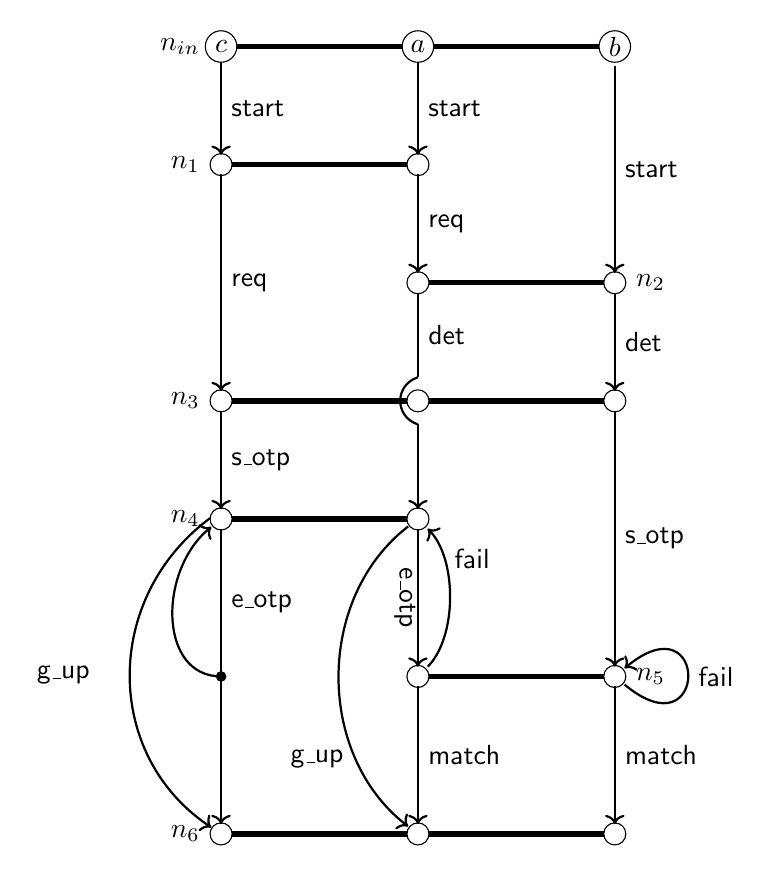
\begin{tikzpicture}

\begin{scope}[line width=2pt]
\draw (0.,0) node [left] {$n_{\text{in}}\,\,$} -- (5,0);
\draw (0.,-1.5) node [left] {$n_{1}\,\,$} -- (2.5,-1.5);
\draw (2.5,-3) -- (5,-3) node [right] {$\,\,n_{2}$};
\draw (0.,-4.5) node [left] {$n_{3}\,\,$} -- (5,-4.5);
\draw (0.,-6) node [left] {$n_{4}\,\,$} -- (2.5,-6);
\draw (2.5,-8) -- (5,-8)  node [right] {\,\,$n_{5}$};
\draw (0.,-10) node [left] {$n_{6}\,\,$} -- (5,-10);
\end{scope}

\begin{scope}[fill=white]
\filldraw  (0,0)  circle (2mm) node (nic) {$c$};
\filldraw  (2.5,0)  circle (2mm) node (nia) {$a$};
\filldraw  (5,0)  circle (2mm) node (nib) {$b$};

\filldraw  (0,-1.5)  circle (1.4mm) node (n1c) {};
\filldraw  (2.5,-1.5)  circle (1.4mm) node (n1a) {};

\filldraw  (2.5,-3)  circle (1.4mm) node (n2a) {};
\filldraw  (5,-3)  circle (1.4mm) node (n2b) {};

\filldraw  (0,-4.5)  circle (1.4mm) node (n3c) {};
\filldraw  (2.5,-4.5)  circle (1.4mm) node (n3a) {};
\filldraw  (5,-4.5)  circle (1.4mm) node (n3b) {};

\filldraw  (0,-6)  circle (1.4mm) node (n4c) {};
\filldraw  (2.5,-6)  circle (1.4mm) node (n4a) {};

\filldraw  (2.5,-8)  circle (1.4mm) node (n5a) {};
\filldraw  (5,-8)  circle (1.4mm) node (n5b) {};

\filldraw  (0,-10)  circle (1.4mm) node (n6c) {};
\filldraw  (2.5,-10)  circle (1.4mm) node (n6a) {};
\filldraw  (5,-10)  circle (1.4mm) node (n6b) {};

\filldraw  [fill=black] (0,-8)  circle (0.6mm) node (v1) {};
\end{scope}

\begin{scope}[thick,->]
\draw (nic) -- (n1c) node [right, midway] {$\mathsf{start}$};
\draw (n1c) -- (n3c) node [right, midway] {$\mathsf{req}$};
\draw (n3c) -- (n4c) node [right, midway] {$\mathsf{s\_otp}$};
\draw (n4c) -- (n6c) node [right, text width = 1.5 cm, near start] {$\mathsf{e\_otp}$};
\draw (0,-8) .. controls  (-0.8,-8) and (-0.8,-6.65) .. (n4c) node [left, midway] {};

\draw (nia) -- (n1a) node [right, midway] {$\mathsf{start}$};
\draw (n1a) -- (n2a) node [right, midway] {$\mathsf{req}$};
\draw (2.5,-4.8) -- (n4a);
\draw (n4a) -- (n5a) node [below=-0.1cm, sloped, midway] {$\mathsf{e\_otp}$};
\draw (n5a) -- (n6a) node [right, text width = 1 cm, midway] {$\mathsf{match}$};
\draw (n5a) .. controls (3,-7.5) and (3,-6.5) .. (n4a) node [right, near end] {$\mathsf{fail}$};
\draw (n4a) .. controls  (1.2,-7) and (1.2,-9) .. (n6a) node [left=-0.3cm, text width = 1 cm, near end] {$\mathsf{g\_up}$};

\draw (nib) -- (n2b) node [right, midway] {$\mathsf{start}$};
\draw (n2b) -- (n3b) node [right, midway] {$\mathsf{det}$};
\draw (n3b) -- (n5b) node [right, text width = 1 cm, midway] {$\mathsf{s\_otp}$};
\draw (n5b) -- (n6b) node [right, text width = 1 cm, midway] {$\mathsf{match}$};
\draw (n5b) .. controls  (6.2,-9) and (6.2,-7) .. (n5b) node [right, midway] {$\mathsf{fail}$};

\draw (n4c) + (-0.14,0.01) .. controls  (-1.5,-7) and (-1.5,-9) .. (n6c) node [left=-0.2cm, text width = 1.25 cm, midway] {$\mathsf{g\_up}$};
\end{scope}

\draw [thick] (n2a) -- (2.5,-4.2) node [right, midway] {$\mathsf{det}$};
\draw [thick] (2.5,-4.2) .. controls (2.2,-4.3) and (2.2,-4.7) .. (2.5,-4.8);
\end{tikzpicture}
\caption{ATM transaction negotiation. Customer ($c$), ATM ($a$), and bank ($b$) coordinate through atomic interactions. Note the hyperarc at $n_4$ for customer $c$ after $\mathsf{e\_otp}$: non-deterministic control flow allows readiness at both $n_4$ (retry) and $n_6$ (completion).}
\label{fig:ATM}
\end{figure}

\paragraph{Behavior.} Starting from $x_0$ where all agents are at $n_{\text{in}}$, outcome $\mathsf{start}$ occurs, moving $c$ and $a$ to $n_1$, and $b$ to $n_2$. Then $n_1$ and $n_2$ eventually both must occur before $n_3$ becomes enabled. The loop structure at $n_4 \to n_5 \to n_4$ models retry behavior when OTP validation fails. The customer can also ``give up" via outcome $\mathsf{g\_up}$, bypassing validation and proceeding directly to completion.

This example will reappear in Chapter~\ref{chap:ltn} when we add timing constraints to model, for instance, OTP expiration deadlines or maximum retry durations.

%---------------------------------------------------------------------------------------------------------------------------------------------

\subsection{Illustrative Examples: Control-Flow Patterns}

Before studying reachability and complexity, we present several examples highlighting non-trivial control-flow phenomena in negotiations. These patterns recur in distributed systems and will later interact with timing constraints in interesting ways.

%--------------------------------------------------------------------------

\subsubsection{Late Binding of Choice}
\label{subsec:neg-late-binding}

Negotiations allow choices made by a subset of agents to constrain future
interactions without being immediately resolved. This
\emph{late binding of choice}, is already illustrated by the pollination example~\ref{}
introduced in Chapter~\ref{chap:intro}. There, the outcome ($gc$ or $ch$) of the environment-related
node ($n_2$) determines whether normal ($n_4$) or early flowering ($n_5$) may occur later, even though
the agents participating in flowering do not take part in the climate decision.
Once the environment outcome is fixed, only the corresponding branch remains
feasible, and executions that mix incompatible branches are impossible.

Late binding of choice allows early, local decisions to propagate constraints
through the negotiation structure, with their effects realised only through
later multiparty interactions rather than immediate global synchronization.
This pattern will later reappear in local-timed negotiations~\ref{}, where relative timing
information accumulated early constrains which interactions are feasible later.
%--------------------------------------------------------------------------
\subsubsection{Example: Implicit Consensus}
\label{subsec:neg-implicit-consensus}

Negotiations can enforce agreement between agents through the structure of feasible
interactions, even in the absence of explicit communication or global
synchronization.

\begin{example}[Implicit consensus]
\label{ex:implicit-consensus}
Let $P=\{p,q,r\}$ and
\[
N=\{n_{pq},\, n_p,\, n_{qr}^0,\, n_{qr}^1,\, n_f\}.
\]
Domains are given by
\[
\dom(n_{pq})=\{p,q\},\quad \dom(n_p)=\{p\},\quad
\dom(n_{qr}^0)=\dom(n_{qr}^1)=\{q,r\},\quad \dom(n_f)=\{p,q,r\}.
\]
At $n_{pq}$ the set of outcomes is $\{0,1\}$. For $b\in\{0,1\}$, define
\[
\delta_p(n_{pq},b)=\{n_p\},\qquad
\delta_q(n_{pq},b)=\{n_{qr}^b\},\qquad
\delta_r(n_{pq},b)=\{n_{qr}^b\}.
\]
Node $n_p$ has a single outcome $x$ with $\delta_p(n_p,x)=\{n_f\}$.
Each node $n_{qr}^b$ has outcome $x$ with
\[
\delta_q(n_{qr}^b,x)=\{n_f\},\qquad
\delta_r(n_{qr}^b,x)=\{n_f\}.
\]
Finally, $n_f$ is terminal.
\end{example}

\paragraph{Observation.}
After the initial interaction at $n_{pq}$, agent $p$ never interacts again with
$q$ or $r$. Nevertheless, the outcome chosen at $n_{pq}$ uniquely determines which
interaction $q$ and $r$ must later execute: either $n_{qr}^0$ or $n_{qr}^1$.
Thus, $q$ and $r$ are forced to agree on a common branch, not through explicit
coordination or message-passing, but because all feasible continuations must be
consistent with the earlier choice. This example illustrates how negotiations can
enforce agreement purely via feasibility constraints—a phenomenon that will later
reappear when timing information is propagated and compared through selective
synchronization.

\subsubsection{Example: Transitive Causality Without Shared Participants}
\label{subsec:neg-causality-no-share}

Causality in negotiations is not restricted to interactions that share agents
directly; it can propagate transitively through the control-flow structure.

\begin{example}[Transitive causality]
\label{ex:causality-no-share}
Let $P=\{p,q,r,s\}$ and
\[
N=\{n_1,\, n_m,\, n_2\}
\]
with domains
\[
\dom(n_1)=\{p,q\},\quad \dom(n_m)=\{q,r\},\quad \dom(n_2)=\{r,s\}.
\]
All nodes have outcome $\{x\}$. Initially,
\[
x_0(p)=x_0(q)=\{n_1\},\qquad x_0(r)=x_0(s)=\emptyset.
\]
Transitions form a chain:
\begin{align*}
\delta_p(n_1,x) &= \emptyset, &
\delta_q(n_1,x) &= \{n_m\}, &
\delta_r(n_1,x) &= \{n_m\}, \\
\delta_q(n_m,x) &= \emptyset, &
\delta_r(n_m,x) &= \{n_2\}, &
\delta_s(n_m,x) &= \{n_2\}, \\
\delta_r(n_2,x) &= \emptyset, &
\delta_s(n_2,x) &= \emptyset.
\end{align*}
\end{example}

\paragraph{Observation.}
Although $\dom(n_1)\cap\dom(n_2)=\emptyset$, node $n_2$ cannot occur before $n_1$ in
any execution. The causal dependency $n_1 \prec n_2$ is transmitted through the
intermediate interaction $n_m$, which shares agents with both. This example shows
that causality in negotiations is a global, structural property rather than a
local one determined solely by shared participants. Such transitive dependencies
will play an important role later when timing constraints and synchronization
effects propagate along chains of interactions.

\begin{figure}[p] % 'p' places these on a separate page, 't' or 'h' for inline
\centering

% --- Example 2: Implicit Consensus ---
\begin{subfigure}[b]{0.45\textwidth}
\centering
\resizebox{\textwidth}{!}{%
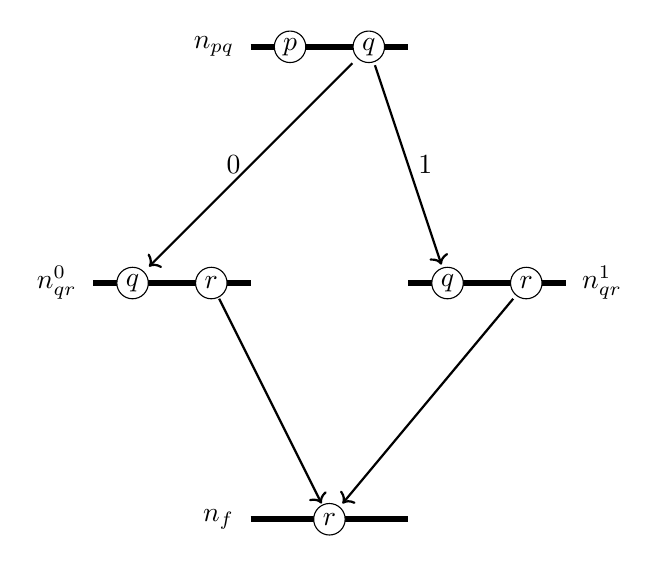
\begin{tikzpicture}
    % Nodes
    \draw[line width=2pt] (2,4) node[left] {$n_{pq}\,$} -- (4,4);
    
    \draw[line width=2pt] (0,1) node[left] {$n_{qr}^0\,$} -- (2,1);
    \draw[line width=2pt] (4,1) -- (6,1) node[right] {$\,n_{qr}^1$};
    
    \draw[line width=2pt] (2,-2) node[left] {$n_f\,$} -- (4,-2);

    % Ports
    \filldraw[fill=white] (2.5,4) circle (2mm) node (p_npq) {$p$};
    \filldraw[fill=white] (3.5,4) circle (2mm) node (q_npq) {$q$};
    
    \filldraw[fill=white] (0.5,1) circle (2mm) node (q_n0) {$q$};
    \filldraw[fill=white] (1.5,1) circle (2mm) node (r_n0) {$r$};
    
    \filldraw[fill=white] (4.5,1) circle (2mm) node (q_n1) {$q$};
    \filldraw[fill=white] (5.5,1) circle (2mm) node (r_n1) {$r$};
    
    \filldraw[fill=white] (3,-2) circle (2mm) node (r_nf) {$r$};

    % Edges
    \draw[->, thick] (q_npq) -- (q_n0) node[midway, left] {$0$};
    \draw[->, thick] (q_npq) -- (q_n1) node[midway, right] {$1$};
    
    \draw[->, thick] (r_n0) -- (r_nf);
    \draw[->, thick] (r_n1) -- (r_nf);
\end{tikzpicture}
}
\caption{\textbf{Implicit Consensus.} $q$ routes control based on $n_{pq}$, forcing $r$ to match.}
\label{fig:implicit_consensus}
\end{subfigure}

\vspace{1cm}

% --- Example 4: Transitive Causality ---
\begin{subfigure}[b]{0.45\textwidth}
\centering
\resizebox{\textwidth}{!}{%
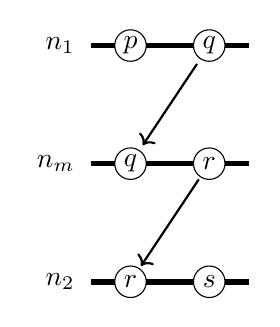
\begin{tikzpicture}
    % Nodes
    \draw[line width=2pt] (0,3) node[left] {$n_1\,$} -- (2,3);
    \draw[line width=2pt] (0,1.5) node[left] {$n_m\,$} -- (2,1.5);
    \draw[line width=2pt] (0,0) node[left] {$n_2\,$} -- (2,0);

    % Ports
    \filldraw[fill=white] (0.5,3) circle (2mm) node (p_n1) {$p$};
    \filldraw[fill=white] (1.5,3) circle (2mm) node (q_n1) {$q$};

    \filldraw[fill=white] (0.5,1.5) circle (2mm) node (q_nm) {$q$};
    \filldraw[fill=white] (1.5,1.5) circle (2mm) node (r_nm) {$r$};

    \filldraw[fill=white] (0.5,0) circle (2mm) node (r_n2) {$r$};
    \filldraw[fill=white] (1.5,0) circle (2mm) node (s_n2) {$s$};

    % Edges
    \draw[->, thick] (q_n1) -- (q_nm); % q flows n1 -> nm
    \draw[->, thick] (r_nm) -- (r_n2); % r flows nm -> n2
\end{tikzpicture}
}
\caption{\textbf{Transitive Causality.} $n_1 \prec n_2$ via shared agents $q,r$, despite disjoint domains.}
\label{fig:transitive_causality}
\end{subfigure}

\caption{Graphical representations of the control-flow examples discussed in Section~\ref{}.}
\label{fig:control_flow_examples}
\end{figure}

%---------------------------------------------------------------------------------------------------------------------------------------------

\subsection{Reachability and complexity results}
\label{sec:complexity}

We briefly summarize known complexity results for negotiations and related models. These results motivate both the use of negotiations as a concurrency formalism and the restrictions studied in later chapters.

\paragraph{General negotiations.}
For unrestricted negotiations, the reachability problem is decidable. However, the reachability graph can be exponential in the size of the negotiation, and several analysis problems are computationally expensive. In particular, soundness and reachability are PSPACE-hard in general.

\paragraph{Acyclic and sound negotiations.}
For important subclasses, the complexity drops significantly. For example, reachability and soundness are decidable in polynomial time for acyclic negotiations and for sound negotiations with restricted control-flow. These results contrast sharply with Petri nets, where even severely restricted classes often retain high complexity.

%add other results
%add 'timed negotiation' results
%---------------------------------------------------------------------------------------------------------------------------------------------

\subsection{Relation to Standard Negotiations with Transformers}
\label{sec:standard-def}

The negotiation model presented in Section~\ref{sec:negotiations} abstracts away internal agent states and transformers. For completeness and to connect with the original literature~\cite{EsparzaDeselNegotiations}, we briefly recall the standard definition and establish equivalence for control-flow properties. For the purposes of this thesis, the internal state evolution carried by transformers plays no role in enabling or disabling interactions.

\paragraph{Standard definition (informal).} In the original model, each agent $p$ has an internal state space $Q_p$ with initial states $Q_{0p}$. An atom $n$ involves parties $P_n$ and has outcomes $R_n$. Each outcome $r$ is associated with a \emph{transformer} $\tau_r$: a left-total relation $\tau_r \subseteq Q_A \times Q_A$ (where $Q_A = \prod_{p \in P} Q_p$) that is a $P_n$-transformer—it only affects states of agents in $P_n$.

When outcome $(n,r)$ occurs, agents in $P_n$ change states according to $\tau_r$, while agents outside $P_n$ remain unchanged. Crucially, \emph{enablement of an atom depends only on readiness}, not on the specific internal states of agents. The choice of outcome is non-deterministic and not restricted by internal states. Transformers determine only how internal states evolve \emph{after} an outcome occurs.

\paragraph{Why the simplification suffices.} Since this thesis focuses on reachability and control-flow properties, internal states are orthogonal: they do not influence which atoms are enabled or which outcomes can occur. All information relevant to reachability is captured by tracking which nodes each agent is ready for—exactly what markings record in our simplified definition.

\paragraph{Equivalence.}
The simplified definition of negotiations used in this thesis is equivalent to the standard definition with internal states and transformers, as far as reachability is concerned. Formally, from a standard negotiation one obtains the simplified model by projecting away internal states and retaining only the next-atom relation, which fully determines enablement and control flow. This simplification is semantic rather than approximate: it preserves the reachability graph exactly. Conversely, any simplified negotiation can be viewed as a standard one by equipping each agent with a trivial one-state internal domain and identity transformers. In both cases, the induced reachability graphs coincide. In both constructions, there is a bijection between reachable markings preserving enabled atoms and outcome occurrences. Occurrence sequences and reachability graphs correspond exactly. Properties expressible in terms of control flow (e.g., reachability, deadlock) are preserved.

%---------------------------------------------------------------------------------------------------------------------------------------------

\subsection{Relation to Petri Nets}
\label{sec:neg-pn}

Negotiations are closely related to a restricted class of Petri nets, and this
relationship is bidirectional. Esparza et al.~\cite{esparza-neg-pn,esparza-neg-ceur}
establish a behavior-preserving translation from negotiations to Petri nets and,
conversely, characterize negotiations as Petri nets satisfying strong structural
constraints.

\paragraph{From negotiations to Petri nets.}
Let $\mathcal{N}=(P,N,\dom,\delta,x_0)$ be a negotiation. One can construct a safe
Petri net $\mathcal{P}_{\mathcal{N}}=(\mathcal{P},\mathcal{T},F,M_0)$ as follows.
For each agent $p\in P$ and each atom $n\in N$ with $p\in\dom(n)$, the net contains a
place $(p,n)$ representing that agent $p$ is ready to engage in atom $n$. The initial
marking $M_0$ places one token in each place $(p,n)$ such that $n\in x_0(p)$.

For each outcome $(n,r)$ of an atom $n$, and for each choice of one input place
$(p,n)$ for every $p\in\dom(n)$, the net contains a transition $t_{n,r}$. The preset
of $t_{n,r}$ consists of the places $(p,n)$ for $p\in\dom(n)$, and its postset
consists of all places $(p,n')$ with $n'\in\delta_p(n,r)$. Firing $t_{n,r}$ consumes
one token from each input place and produces tokens according to the transition
function of the negotiation.

This construction preserves reachability: a marking is reachable in
$\mathcal{N}$ if and only if the corresponding marking is reachable in
$\mathcal{P}_{\mathcal{N}}$. Moreover, two outcomes are concurrently enabled in
$\mathcal{N}$ if and only if the corresponding transitions are independent in
$\mathcal{P}_{\mathcal{N}}$.

\paragraph{Structural characterization.}
The Petri nets obtained from negotiations satisfy strong restrictions. They are
safe, and their places are partitioned by agents, so that each token represents the
local control state of exactly one agent. Synchronization occurs only at transitions
whose preset contains exactly one place per participating agent. In particular,
tokens are never merged or split across agents, and no place is shared between
agents.

Conversely, Esparza et al.~\cite{esparza-neg-ceur} show that every Petri net satisfying
these structural conditions corresponds to a negotiation, in the sense that its
behavior can be captured by an interaction-centric model with atoms and outcomes.
Thus, negotiations form a well-defined fragment of safe workflow Petri nets in which
control flow is mediated exclusively by multiparty interactions.

\paragraph{Consequences.}
The restricted synchronization discipline of negotiations distinguishes them from
general Petri nets and underlies their improved algorithmic properties. These
structural features will be crucial when extending the model with local timing
constraints in later chapters.

%---------------------------------------------------------------------------------------------------------------------------------------------

\section{Timed Automata}
\label{sec:timed-automata}

Timed automata~\cite{AlurDillTA} extend finite automata with real-valued clock variables that evolve continuously with time. They provide the standard framework for modeling and verifying real-time systems, and form the semantic foundation for the timing aspects of local-timed negotiations.

We briefly recall their definition, operational semantics, and the region-based decidability result for reachability, which will serve as a conceptual template for later constructions. This material is standard; we include it to establish notation and to highlight which techniques transfer (or fail to transfer) to local-timed negotiations.

%---------------------------------------------------------------------------------------------------------------------------------------------

\subsection{Syntax and Semantics}

We work in dense time over the non-negative reals $\mathbb{R}_{\geq 0}$. All clocks evolve synchronously with global time in standard timed automata.

\paragraph{Clock constraints.} Let $X$ be a finite set of \emph{clocks}. A \emph{clock valuation} is a function $v : X \to \mathbb{R}_{\geq 0}$. For $\delta \in \mathbb{R}_{\geq 0}$, we write $v + \delta$ for the valuation $(v + \delta)(x) = v(x) + \delta$ (uniform time elapse). For $Y \subseteq X$, we write $[Y]v$ for the valuation that resets clocks in $Y$ to zero: $([Y]v)(x) = 0$ if $x \in Y$, and $([Y]v)(x) = v(x)$ otherwise.

The set of \emph{clock constraints} over $X$, denoted $\mathcal{C}(X)$, is defined by the grammar:
\[
g ::= x \bowtie c \mid g \wedge g
\]
where $x \in X$, $c \in \mathbb{N}$, and $\bowtie \in \{<, \leq, =, \geq, >\}$. A valuation $v$ \emph{satisfies} constraint $g$, written $v \models g$, if $g$ evaluates to true when each clock $x$ is replaced by $v(x)$.

\begin{definition}[Timed automaton]
\label{def:timed-automaton}
A \textsf{timed automaton} (TA) is a tuple $\mathcal{A} = (Q, \S, X, T, q_0, \text{Acc})$ where:
\begin{itemize}
\item $Q$ is a finite set of \emph{states} (or \emph{locations}),
\item $\S$ is a finite \emph{alphabet} of actions,
\item $X$ is a finite set of \emph{clocks},
\item $q_0 \in Q$ is the \emph{initial state},
\item $\text{Acc} \subseteq Q$ is the set of \emph{accepting states},
\item $T \subseteq Q \times \S \times \mathcal{C}(X) \times 2^X \times Q$ is a finite set of \emph{transitions}. A transition $(q, a, g, R, q') \in T$ has source state $q$, action label $a$, guard $g$, reset set $R$, and target state $q'$.
\end{itemize}
\end{definition}

\paragraph{Semantics.} The behavior of $\mathcal{A}$ is given by an infinite-state transition system whose \emph{configurations} are pairs $(q, v)$ consisting of a state $q \in Q$ and a valuation $v : X \to \mathbb{R}_{\geq 0}$. The \emph{initial configuration} is $(q_0, \mathbf{0})$ where $\mathbf{0}$ denotes the valuation assigning zero to all clocks.

There are two kinds of transitions:
\begin{itemize}
\item \textbf{Delay transitions:} $(q, v) \xrightarrow{\delta} (q, v + \delta)$ for any $\delta \in \mathbb{R}_{\geq 0}$. Time elapses uniformly for all clocks.
\item \textbf{Action transitions:} $(q, v) \xrightarrow{a} (q', v')$ if there exists a transition $(q, a, g, R, q') \in T$ such that $v \models g$ and $v' = [R]v$. The guard must be satisfied, and clocks in $R$ are reset.
\end{itemize}

A \emph{run} is a finite or infinite alternating sequence of delay and action transitions starting from the initial configuration:
\[
(q_0, \mathbf{0}) \xrightarrow{\delta_0} (q_0, v_0) \xrightarrow{a_0} (q_1, v_1) \xrightarrow{\delta_1} (q_1, v_1') \xrightarrow{a_1} (q_2, v_2) \xrightarrow{\delta_2} \cdots
\]
We often write $(q, v) \xrightarrow{\delta, a} (q', v')$ to denote a delay $\delta$ followed immediately by action $a$. A run is \emph{accepting} if it reaches some configuration $(q_f, v)$ with $q_f \in \text{Acc}$.

\begin{definition}[Reachability problem for TA]
Given a timed automaton $\mathcal{A}$ and a target state $q_{\text{target}} \in Q$, the \textsf{reachability problem} asks: does there exist an accepting run reaching some configuration $(q_{\text{target}}, v)$?
\end{definition}

%---------------------------------------------------------------------------------------------------------------------------------------------

\subsection{Region Abstraction and Decidability~\cite{}}

For this thesis, regions serve as the main conceptual tool for proving decidability and establishing complexity bounds, in particular as a reference point when extending negotiations with local time. We therefore briefly recall the region abstraction for timed automata, focusing on the properties needed later.

Since the transition system of a timed automaton is infinite, the standard approach is to construct a finite abstraction by grouping clock valuations that are indistinguishable with respect to future behaviour. Concretely, two valuations are grouped together if they enable the same transitions and allow the same sequences of discrete states to be reached, possibly with different delays. This yields a finite partition of the valuation space into regions, and a corresponding finite region graph obtained by combining regions with control states. For reachability, the exact delays are irrelevant; only the existence of a run following a given sequence of transitions matters.

Let $X$ be a finite set of clocks. Let $M : X \xra N \cup \{-\infty\}$ be a bound function that associates a constant $M_x \in N$ to every clock $x$.

\begin{definition}[Region equivalence \cite{}]
Two valuations $v, v' \in \Rpos$ are region equivalent w.r.t. $M$, denoted $v \sim_M v'$ iff for every $x, y \in X$:
\begin{itemize}
	\item $v(x) > M_x$ iff $v'(x) > M_x$;
	\item if $v(x) \leq M_x$, then $\lceil v(x) \rceil = \lceil v'(x) \rceil$;
	\item if $v(x) \leq M_x$, then $\{v(x)\} = 0$ iff $\{v'(x)\} = 0$;
	\item if $v(x) \leq M_x$ and $v(y) \leq M_y$ then $\{v(x)\} \leq \{v(y)\}$ iff $\{v'(x)\} \leq \{v'(y)\}$.
\end{itemize}
\end{definition}

Given a timed automaton $A$, a bound function is obtained by choosing for a clock $x$, the maximum constant appearing in a guard involving $x$. Then, the first three conditions in the above definition ensure that the two valuations satisfy the same guards. The last one enforces that for every $\d \in \Rpos$ there is $\d' \in \Rpos$, such that valuations $v + \d$ and $v' + \d'$ satisfy the same guards.

\begin{definition}[Regions \cite{}]
Let $M : X \xra{} \N \cup \{-\infty\}$ be a bound function. A region is an equivalence class of $\sim_M$. We write $[v]^M$ for the region of $v$, and $\calR_M$ for the set of all regions with respect to $M$.
\end{definition}

Figure~\ref{} shows the division into regions when there are two clocks $x$ and $y$. We also give below a constructive definition of regions which would be useful to estimate the number of regions.

\begin{definition}[Region: constructive definition \cite{}]
A region with respect to bound function $M$ is a set of valuations specified as follows:
\begin{itemize}
	\item for each clock $x \in X$, one constraint from the set: $\{x = c \mid c = 0, \dots, M_x\} \cup \{c - 1 < x < c \mid c = 1, \dots, M_x\} \cup \{x > M_x\}$
	\item for each pair of clocks $x, y$ having interval constraints: $c - 1 < x < c$ and $d - 1 < y < d$, it is specified if $\{x\}$ is less than, equal to or greater than $\{y\}$.
\end{itemize}
\end{definition}

If $r$ is a region then we will write $r \models g$ to mean that every valuation in $r$ satisfies the guard $g$. It is straightforward to see that if a valuation $v \in r$ satisfies the guard $g$, then every valuation $v' \in r$ satisfies $g$. We will now show the other property with respect to time-elapse mentioned above.

\begin{lemma}
Let $v, v'$ be valuations such that $v' \sim v$. Then, for all $\d \in \Rpos$ there exists a $\d' \in \Rpos$ such that $v' + \d' \sim_M v + \d$.
\end{lemma}

\begin{proof}
Let $v' \sim v$ and fix $\d \in \Rpos$. We construct $\d'$. Put $\lceil \d' \rceil$ to be $\lceil \d \rceil$. Clearly, we have $v' + \lceil \d' \rceil \sim_M \lceil \d \rceil$: that is, valuations $v' + \lceil \d' \rceil$ and $v + \lceil \d \rceil$ have the same integral parts and the same ordering of fractional parts (modulo $M$). Let $x_1 \lessdot_1 x_2 \lessdot_2 \cdots \lessdot_{k - 1} x_k$ be the ordering of fractional parts of clocks less than $M$ in both the valuations. Here $\lessdot$ denotes either $<$ or $=$. 

From $v + \lceil \d \rceil$, elapsing a fractional amount $\{\d\}$ might move some of the clocks up to the next integer. Let $x_j, x_{j + 1}, \dots, x_k$ be the clocks that have their integral values increased from $v + \lceil \d \rceil$ due to the fractional elapse $\{\d\}$. Thanks to the denseness of the real line, one can choose $\{\d'\}$ between the fractional values of clocks $x_{j - 1}$ and $x_j$ in $v' + \lceil \d' \rceil$ so that $v' + \d'$ has the same integers as $v + \d$ and the same ordering of fractional parts (modulo $M$).
\end{proof}

Given a bound function $M$, the number of regions in $\calR_M$ is finite. Once this finite partition of the valuations is obtained, we proceed to define a finite graph built from these regions, that captures the behaviour of the timed automaton. For an automaton $A$, to define its region graph, we consider a bound function $M_A$ that is obtained from the automaton’s definition.

\begin{definition}[Maximal bounds]
Given an automaton $A$, the maximal bounds function $M_A: X \xra{} \N \cup \{-\infty\}$ associates to each clock $x$ the biggest constant appearing in a guard of the automaton that involves $x$. If there is no guard involving $x$, then $M_A(x)$ is assigned $-\infty$.
\end{definition}

We define the region graph of an automaton $A$ using the $\sim_{M_A}$ relation. Note that in class, we used the terminology region automaton. As we are not interested in the language accepted by this automaton, and instead we care if there is a path to the accepting state, we will stick to calling this a region graph.

\begin{definition}[Region graph \cite{}]
Nodes of the region graph denoted by $RG(A)$ are of the form $(q, r)$ for $q$ a state of $A$ and $r \in \calR_{M_A}$ a region. There is a transition $(q, r) \xra{t} (q', r')$ if there are $v \in r, \d \in \Rpos$ and $v' \in r'$ with $(q, v) \xra{\d, t} (q', v')$. The initial node of the region graph is $(q_0, [0]_{\sim_{M_A}})$ where $[0]_{\sim_{M_A}}$ represents the region to which the initial valuation $0$ belongs to. A node $(q, r)$ is said to be an accepting node if $q \in Acc$.
\end{definition}

A key property of region graphs is pre-stability, which ensures that transitions are representative of all valuations in a region.

\begin{lemma}[Pre-stability of regions]
\label{lem:prestability}
Let $A$ be a timed automaton and let $RG(A)$ be its region graph. Transitions in $RG(A)$ are pre-stable: for every transition $(q,r)\xra{t}(q',r')$ in $RG(A)$ and every valuation $v \in r$, there exist $\d \in \Rpos$ and a valuation $v' \in r'$ such that $(q,v)\xra{\d,t}(q',v')$ in $A$.
\end{lemma}

\begin{proof}
Fix a transition $(q,r)\xra{t}(q',r')$ in $RG(A)$. By definition of the region graph, there exist $v_0 \in r$, $\d_0 \in \Rpos$ and $v_0' \in r'$ such that $(q,v_0)\xra{\d_0,t}(q',v_0')$ is a valid step in $A$. Let $v \in r$ be arbitrary. By the time-elapse property of region equivalence (Lemma~\ref{lem:time-elapse-region} in your text), there exists $\d \in \Rpos$ such that $v+\d$ lies in the same region as $v_0+\d_0$. Since valuations in the same region satisfy the same guards, $v+\d$ satisfies the guard of $t$. Let $v' := [R](v+\d)$ be the valuation obtained by applying the reset set $R$ of transition $t$. Region equivalence is preserved under resets, hence $v' \in r'$. Therefore $(q,v)\xra{\d,t}(q',v')$ is a valid step of $A$ with $v' \in r'$. 
\end{proof}

The following lemma is a direct consequence of the pre-stability property.

\begin{lemma}
Every path in $RG(A)$ is an abstraction of a run of $A$, and conversely, every run of $A$ is an instantiation of a path in $RG(A)$.
\end{lemma}

The above lemma shows that the region graph is sound and complete for state reachability.

\begin{theorem}[\cite{}]
Automaton $A$ has an accepting run iff there is a path in the region graph $RG(A)$ starting from its initial node to an accepting node.
\end{theorem}

While this theorem gives an algorithm for solving our problem, it turns out that this method is very impractical. The number of regions obtained using a bound function $M$ is $\calO (|X|! \cdot 2^{|X|} \cdot \prod_{x \in X} (2M_x + 2))$ \cite{} and constructing all of them, or even searching through them on-the-fly, has proved to be very costly. Understanding why region abstractions work in the global-time setting is crucial to appreciating the techniques that are required in local-timed negotiations. The crucial assumption underlying regions is the existence of a single global time along which all clocks evolve uniformly.

%---------------------------------------------------------------------------------------------------------------------------------------------

\section{Networks of Timed Automata}
\label{sec:networks-ta}

Real systems consist of multiple concurrent components, each with its own state space and timing behavior. \emph{Networks of timed automata} model such systems as collections of timed automata that evolve concurrently and synchronize on shared actions.

\begin{definition}[Network of timed automata]
\label{def:network}
A \textsf{network of timed automata} with $k$ processes is a tuple $(\mathcal{A}_1, \ldots, \mathcal{A}_k)$ where each $\mathcal{A}_p = (Q_p, \S_p, X_p, T_p, q_p^0)$ is a timed automaton (we omit accepting states for simplicity). We require:
\begin{itemize}
\item State spaces are pairwise disjoint: $Q_i \cap Q_j = \emptyset$ for $i \neq j$,
\item Clock sets are pairwise disjoint: $X_i \cap X_j = \emptyset$ for $i \neq j$.
\end{itemize}
We write $Q = \prod_{p=1}^k Q_p$, $\S = \bigcup_{p=1}^k \S_p$, and $X = \bigcup_{p=1}^k X_p$.
\end{definition}

For each action $a \in \S$, define its \emph{domain} $\text{dom}(a) = \{p \mid a \in \S_p\}$: the set of processes that participate in $a$. An action with $|\text{dom}(a)| > 1$ is a \emph{synchronization action}.

\paragraph{Global-time semantics.} The semantics of a network is given by a global transition system where configurations are pairs $(q, v)$ with $q \in Q$ and $v : X \to \mathbb{R}_{\geq 0}$. The initial configuration is $(q^0, \mathbf{0})$ where $q^0 = (q_1^0, \ldots, q_k^0)$.

Transitions are of two kinds:
\begin{itemize}
\item \textbf{Global delay:} $(q, v) \xrightarrow{\delta} (q, v + \delta)$ for any $\delta \in \mathbb{R}_{\geq 0}$. All clocks advance uniformly.
\item \textbf{Action step:} $(q, v) \xrightarrow{a} (q', v')$ if there exists a set of transitions $\{(q_p, a, g_p, R_p, q_p')\}_{p \in \text{dom}(a)}$ in the respective automata $\mathcal{A}_p$ such that:
\begin{itemize}
\item States of processes in $\text{dom}(a)$ change: $q(p) = q_p$ and $q'(p) = q_p'$ for $p \in \text{dom}(a)$; states of other processes remain unchanged: $q'(p) = q(p)$ for $p \notin \text{dom}(a)$,
\item All guards are satisfied: $v \models g_p$ for all $p \in \text{dom}(a)$,
\item Clocks in the union of reset sets are reset: $v' = [\bigcup_{p \in \text{dom}(a)} R_p] v$.
\end{itemize}
\end{itemize}

A \emph{run} is a sequence of transitions starting from the initial configuration. We write $(q_0, v_0) \xrightarrow{w} (q_n, v_n)$ if there exists a run executing action sequence $w = a_1 \cdots a_n$ with appropriate delays.

\begin{definition}[Reachability for networks]
Given a network and a target global state $q_{\text{target}} \in Q$, does there exist a run reaching some configuration $(q_{\text{target}}, v)$?
\end{definition}

\paragraph{Decidability and complexity.} Reachability remains PSPACE-complete (as for timed automata). The region construction extends naturally: we partition the global valuation space using the product of bounds from all automata. However, the number of regions grows exponentially in both the number of clocks and the maximal constant, making the construction even less practical than for single automata.

\paragraph{The global-time assumption.} A crucial feature of this semantics is that time is \emph{global}: all clocks advance uniformly during delay transitions. Synchronization on action $a$ is instantaneous—no time elapses during an action step. This assumption simplifies analysis but may be unrealistic for distributed systems where components operate asynchronously with independent local timers.

\paragraph{Toward local time.} An alternative semantics for networks, called \emph{local-time semantics}, allows each process to have its own notion of elapsed time~\cite{}. Delays need not be uniform across processes. Synchronization can be modeled as aligning local times at interaction points. This semantic shift has been studied for networks of timed automata~\cite{LocalTimeTA} and forms the conceptual basis for local-timed negotiations, which we introduce in Chapter~\ref{chap:ltn}.

The key difference: in global-time semantics, a single global clock enforces uniform progress; in local-time semantics, each process progresses independently, and synchronization becomes an explicit mechanism for coordination rather than an implicit consequence of shared global time.

\section{Takeaway}
From negotiations, we retain an interaction-centric view of concurrency in which
synchronization is explicit and control flow is captured by markings rather than by
local states. From timed automata, we retain quantitative timing constraints in the
form of clocks, guards, resets, and the idea of finite abstractions such as regions.
Local-timed negotiations combine these elements while deliberately rejecting the
assumption of a single global time that underpins classical decidability results for
timed automata. This separation allows us to study precisely how timing and
synchronization interact to determine the boundary between decidability and
undecidability.

%---------------------------------------------------------------------------------------------------------------------------------------------

\section{Summary and Perspective}
\label{sec:summary}

This chapter established the formal foundations on which the remainder of the thesis
is built. We reviewed two complementary models:

\begin{itemize}
\item \textbf{Negotiations} provide an interaction-centric model of concurrency in
      which multiparty synchronization is primitive. We presented a control-flow-
      oriented formulation suitable for reachability analysis, illustrated the model
      through examples highlighting non-trivial concurrency patterns, and discussed
      its relationship to Petri nets.

\item \textbf{Timed automata} extend finite automata with real-valued clocks and form
      the standard framework for modeling real-time systems. We recalled their
      semantics, the region-based decidability result for reachability, and the
      PSPACE-completeness of the reachability problem.

\item \textbf{Networks of timed automata} model concurrent real-time systems via
      synchronization on shared actions, relying on a global-time semantics with
      uniform clock progression.
\end{itemize}

\subsection{Synthesizing the Models: Toward Local-Timed Negotiations}

We now synthesize these models into the central object of this thesis:
\emph{local-timed negotiations (LTNs)}, which combine the interaction-centric control
structure of negotiations with quantitative timing constraints inspired by timed
automata.

\subsection{Why synthesize these models?}

Negotiations make concurrency explicit through their interaction structure: atoms
involving disjoint sets of agents can occur independently, while shared agents enforce
synchronization. However, negotiations are untimed, limiting their applicability to
systems where quantitative timing constraints such as delays, deadlines, and timeouts
are essential.

Timed automata, by contrast, provide expressive timing mechanisms and decidability via
region abstractions, but even in networks of timed automata, time is global and
concurrency is represented only through interleavings. This global-time assumption
both obscures true independence and contributes to state-space explosion.

\paragraph{Key design decisions.}
Local-timed negotiations combine the following ingredients:
\begin{itemize}
\item \emph{Interaction-centric control flow:} control flow is determined by
      multiparty interactions and their outcomes, making synchronization and
      independence explicit.
\item \emph{Local time progress:} each agent is equipped with its own real-valued
      clock that may advance independently.
\item \emph{Selective time synchronization:} interactions may or may not synchronize
      the local times of their participants.
\item \emph{Quantitative timing constraints:} guards and resets constrain when
      interactions may occur.
\end{itemize}

This combination is not incremental. Moving from a single global clock to locally
evolving time fundamentally changes the semantics: classical region abstractions rely
on uniform time elapse and therefore do not apply directly. Reachability in an LTN asks
whether a target marking can be reached via a sequence of interactions that respects
both control-flow constraints and timing constraints, requiring new techniques to
recover decidability.

\paragraph{Challenges ahead.}
As shown in Chapter~\ref{chap:ltn}, reachability is undecidable for general LTNs that
mix time-synchronizing and non-synchronizing atoms. Decidability can nevertheless be
recovered for restricted fragments by imposing semantic or structural constraints,
including synchronization-free LTNs, fully-synchronizing LTNs, drift-bounded LTNs, and
connectedly-communicating LTNs. The remainder of the thesis explores these fragments
and develops the techniques required to analyze them.

%---------------------------------------------------------------------------------------------------------------------------------------------

\section{Coming Next}

In Chapter~\ref{chap:ltn}, we introduce local-timed negotiations formally, define their
syntax and local-time semantics, and illustrate their modeling power through examples.
We then establish the main negative result: reachability is undecidable for general
LTNs. This result motivates the study of restricted fragments in subsequent chapters,
where decidability is recovered through carefully chosen semantic and structural
constraints.

%__________________________________________________________________________________

\chapter{Local-Timed Negotiations}
\label{chap:ltn}

Chapter~\ref{chap:preliminaries} recalled \emph{negotiations} as an
interaction-centric model of concurrency, and \emph{timed automata} as a standard
framework for real-time constraints.  This chapter introduces
\emph{local-timed negotiations} (LTNs), which equip negotiations with local clocks
and a local-time semantics.  Additionally, LTNs allow \emph{explicit}
synchronization to be enforced at selected negotiation nodes, which is crucial
both for modeling and for expressiveness.

\section{Motivation: Why Local Time?}

\paragraph{The inadequacy of global time.} Networks of timed automata (Section~\ref{sec:networks-ta}) assuming \emph{global time}, i.e., all clocks advance uniformly during delay transitions, and synchronization is instantaneous is inadequate to represents distributed reality for three main reasons:

\begin{itemize}
  \item \textbf{Local clocks:} in realistic distributed protocols, agents progress
        at different rates due to clock drift, computation time, and network
        delays.
  \item \textbf{Partial synchrony:} real systems combine tightly synchronized
        interactions with loosely coupled, independent computation.
  \item \textbf{Agent-centric timing:} timing constraints are often relative to an
        agent’s own actions (e.g.\ completing a workflow within a fixed time after
        initiation), which is awkward to express using a single global timeline.
\end{itemize}

\paragraph{The local-time perspective.} Local-timed negotiations adopt a fundamentally different view: each agent $p$ has a \emph{reference clock} $t_p$ that measures its local elapsed time. Between interactions, agents progress independently—one agent may experience 5 time units while another experiences only 2. At interactions (negotiation nodes), agents coordinate by selecting outcomes that respect their local clock constraints (guards). 

Crucially, LTNs introduce \emph{explicit synchronization} as a modeling choice:
selected nodes may require that participating agents’ reference clocks are equal
when the interaction occurs.  This captures scenarios where coordination demands
temporal alignment, such as simultaneous authentication or tightly coupled sensor
fusion.

\paragraph{What we gain.} This synthesis yields several benefits:

\begin{itemize}
\item \textbf{Explicit concurrency}: The negotiation structure makes independence and causality transparent. Actions involving disjoint agents can occur concurrently without artificial interleaving.

\item \textbf{Agent-centric timing}: Each agent tracks its own deadlines, timeouts, and response times via local clocks, more naturally modeling distributed systems than shared global clocks.

\item \textbf{Selective synchronization}: Synchronizing nodes explicitly capture coordination points where temporal alignment matters, while unsynchronized nodes allow agents to drift.

\item \textbf{Rich expressiveness}: As we'll see, LTNs can model behaviors impossible in purely global-time or purely asynchronous settings, including causal enforcement through timing and non-regular untimed languages.
\end{itemize}

\paragraph{What we sacrifice.} This expressiveness comes at a cost: \emph{unrestricted LTNs have undecidable reachability}. The combination of unbounded clock drift and explicit synchronization creates computational power equivalent to counter machines. The remainder of this thesis identifies restrictions that recover decidability while preserving modeling advantages.

\paragraph{Chapter roadmap.} Section~\ref{sec:ltn-example-informal} introduces LTNs informally through a running example. Section~\ref{sec:ltn-def} provides formal definitions. Section~\ref{sec:ltn-semantics} develops the operational semantics. Section~\ref{sec:ltn-expressiveness} explores expressiveness phenomena unique to local time. Section~\ref{sec:ltn-undec} proves undecidability of reachability. Section~\ref{sec:ltn-summary} synthesizes the main messages and previews the decidable fragments studied in Part~II.

%---------------------------------------------------------------------------------

\section{Related work}
\label{sec:ltn-related}

Negotiations were introduced by Esparza et al.~\cite{DBLP:conf/concur/EsparzaD13,DBLP:journals/acta/DeselEH19}
and admit efficient analysis for several subclasses~\cite{DBLP:journals/lmcs/EsparzaKMW18,DBLP:conf/lics/EsparzaMW17}.
Timed negotiations, which associate durations with outcomes of atomic
negotiations, were studied in~\cite{DBLP:conf/fossacs/AkshayGHM20}; we provide a
detailed comparison with LTNs below.

Local-time semantics for networks of timed automata originates
in~\cite{DBLP:conf/concur/BengtssonJLY98} and has recently been used for
zone-based verification~\cite{DBLP:conf/concur/GovindHSW19,DBLP:conf/lics/0001HSW22}
and B\"uchi reachability~\cite{DBLP:conf/concur/HerbreteauSW22}.  In contrast to
NTA, where shared actions enforce synchronization by design, LTNs start from a
local-time view and offer synchronization as a modeling choice.

\subsection{Comparison with Timed Negotiations~\cite{DBLP:conf/fossacs/AkshayGHM20}}
\label{subsec:ltn-vs-tn}

Timed negotiations~\cite{DBLP:conf/fossacs/AkshayGHM20} extend negotiations
by associating durations with outcomes of atomic negotiations.
Time progress is modelled by assigning durations to individual interactions,
which determine when subsequent negotiations become available.

In contrast, LTNs adopt a clock-based semantics inspired by timed automata,
where time elapses independently of interactions and can be constrained
across multiple negotiations.  This difference has several consequences.
First, LTNs can naturally express timing constraints that relate distinct
interactions, such as deadlines or response-time constraints spanning an
entire workflow.  Second, LTNs allow agents to accumulate and compare local
time through explicit synchronization nodes, whereas timed negotiations
lack a mechanism for comparing temporal progress across interactions.

From an algorithmic perspective, these additional features strictly
increase expressive power: as shown in Section~\ref{sec:ltn-undec},
location-reachability is undecidable for LTNs, whereas timed negotiations
retain decidability for basic analysis problems.  This contrast highlights
the trade-off between expressiveness and tractability when extending
negotiations with time.

Viewed together, timed negotiations and LTNs represent complementary
points in the design space: the former favor tractable timing of
individual interactions, while the latter prioritize expressive,
agent-centric temporal reasoning across interactions.

%---------------------------------------------------------------------------------

\section{Introducing Local-Timed Negotiations: An Informal Example}
\label{sec:ltn-example-informal}

Before formal definitions, we introduce LTNs through an extended version of the ATM transaction example from Chapter~\ref{chap:preliminaries}, now enhanced with timing constraints.

\subsection{Scenario: ATM Transaction with Timeouts}

Recall the basic workflow: a customer ($c$) resets their ATM PIN using a one-time password (OTP) sent by the bank ($b$) through the ATM machine ($a$). We now add realistic timing requirements:

\begin{enumerate}
\item \textbf{Customer timeout}: The customer wants the entire transaction (from request to completion) to take at most 10 time units. If this deadline is exceeded, the customer gives up.

\item \textbf{Bank security policy}: The bank requires that at most 3 time units elapse between sending the OTP and validating it (to prevent replay attacks). Failed validation attempts must also respect this 3-unit window.

\item \textbf{Local time progression}: The customer, ATM, and bank may experience different amounts of elapsed time between interactions due to processing delays, network latency, or user hesitation.
\end{enumerate}

\subsection{Modeling with Local Clocks}

Figure~\ref{fig:ATM} depicts this scenario as a local-timed negotiation. The basic structure follows the untimed negotiation from Chapter~\ref{chap:preliminaries}, augmented with timing annotations:

\begin{figure}[t]
  \centering
  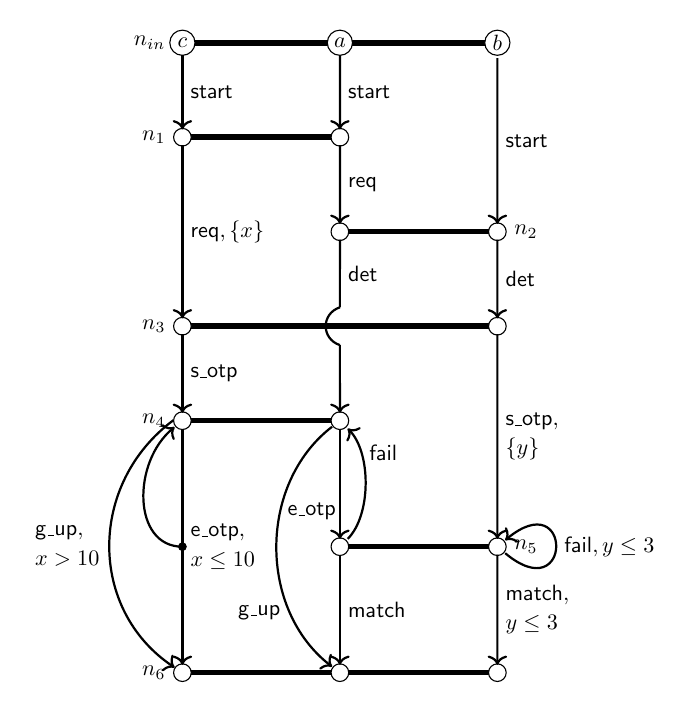
\begin{tikzpicture}[scale=0.8, every node/.style={transform shape}]

\begin{scope}[line width=2pt]
  \draw (0.,0) node [left] {$n_{\text{in}}\,\,$} -- (5,0); 
  \draw (0.,-1.5) node [left] {$n_{1}\,\,$} -- (2.5,-1.5); 
  \draw (2.5,-3) -- (5,-3) node [right] {$\,\,n_{2}$}; 
  \draw (0.,-4.5) node [left] {$n_{3}\,\,$} -- (5,-4.5); 
  \draw (0.,-6) node [left] {$n_{4}\,\,$} -- (2.5,-6); 
  \draw (2.5,-8) -- (5,-8) node [right] {\,\,$n_{5}$}; 
  \draw (0.,-10) node [left] {$n_{6}\,\,$} -- (5,-10);
\end{scope}

\begin{scope}[fill=white]
  \filldraw (0,0) circle (2mm) node (nic) {$c$}; 
  \filldraw (2.5,0) circle (2mm) node (nia) {$a$}; 
  \filldraw (5,0) circle (2mm) node (nib) {$b$};

  \filldraw (0,-1.5) circle (1.4mm) node (n1c) {}; 
  \filldraw (2.5,-1.5) circle (1.4mm) node (n1a) {};

  \filldraw (2.5,-3) circle (1.4mm) node (n2a) {}; 
  \filldraw (5,-3) circle (1.4mm) node (n2b) {};

  \filldraw (0,-4.5) circle (1.4mm) node (n3c) {}; 
  \filldraw (5,-4.5) circle (1.4mm) node (n3b) {};

  \filldraw (0,-6) circle (1.4mm) node (n4c) {}; 
  \filldraw (2.5,-6) circle (1.4mm) node (n4a) {};

  \filldraw (2.5,-8) circle (1.4mm) node (n5a) {}; 
  \filldraw (5,-8) circle (1.4mm) node (n5b) {};

  \filldraw (0,-10) circle (1.4mm) node (n6c) {}; 
  \filldraw (2.5,-10) circle (1.4mm) node (n6a) {}; 
  \filldraw (5,-10) circle (1.4mm) node (n6b) {};

  \filldraw [fill=black] (0,-8) circle (0.6mm) node (v1) {};
\end{scope}

\begin{scope}[thick,->]
  \draw (nic) -- (n1c) node [right, midway] {$\mathsf{start}$}; 
  \draw (n1c) -- (n3c) node [right, midway] {$\mathsf{req}, \{x\}$}; 
  \draw (n3c) -- (n4c) node [right, midway] {$\mathsf{s\_otp}$}; 
  \draw (n4c) -- (n6c) node [right, text width = 1.2 cm, midway] {$\mathsf{e\_otp},$ $x\leq10$}; 
  \draw (0,-8) .. controls (-0.8,-8) and (-0.8,-6.65) .. (n4c);

  \draw (nia) -- (n1a) node [right, midway] {$\mathsf{start}$}; 
  \draw (n1a) -- (n2a) node [right, midway] {$\mathsf{req}$}; 
  \draw (2.5,-4.8) -- (n4a); 
  \draw (n4a) -- (n5a) node [left=-0.3cm, text width = 1 cm, near end] {$\mathsf{e\_otp}$}; 
  \draw (n5a) -- (n6a) node [right, text width = 1 cm, midway] {$\mathsf{match}$}; 
  \draw (n5a) .. controls (3,-7.5) and (3,-6.5) .. (n4a) node [right, near end] {$\mathsf{fail}$}; 
  \draw (n4a) .. controls (1.2,-7) and (1.2,-9) .. (n6a) node [left=-0.3cm, text width = 1 cm, near end] {$\mathsf{g\_up}$};

  \draw (nib) -- (n2b) node [right, midway] {$\mathsf{start}$}; 
  \draw (n2b) -- (n3b) node [right, midway] {$\mathsf{det}$}; 
  \draw (n3b) -- (n5b) node [right, text width = 1 cm, midway] {$\mathsf{s\_otp},$ $\{y\}$}; 
  \draw (n5b) -- (n6b) node [right, text width = 1 cm, midway] {$\mathsf{match},$ $y\leq3$}; 
  \draw (n5b) .. controls (6.2,-9) and (6.2,-7) .. (n5b) node [right, midway] {$\mathsf{fail}, y\leq3$};

  \draw (n4c) + (-0.14,0.01) .. controls (-1.5,-7) and (-1.5,-9) .. (n6c) node [left=-0.2cm, text width = 1.25 cm, midway] {$\mathsf{g\_up},$ $x > 10$};
\end{scope}

\draw [thick] (n2a) -- (2.5,-4.2) node [right, midway] {$\mathsf{det}$}; 
\draw [thick] (2.5,-4.2) .. controls (2.2,-4.3) and (2.2,-4.7) .. (2.5,-4.8);
\end{tikzpicture}
\caption{ATM transaction as a local-timed negotiation. Customer $c$ has local clock $x$ (reset at $\mathsf{req}$, checked at $\mathsf{e\_otp}$ and $\mathsf{g\_up}$). Bank $b$ has local clock $y$ (reset at $\mathsf{s\_otp}$, checked at $\mathsf{match}$ and $\mathsf{fail}$). Annotations like "$x \leq 10$" are guards; "$\{x\}$" indicates clock reset.}
\label{fig:ATM}
\end{figure}

\paragraph{Agent local clocks.} Each agent maintains local clocks:
\begin{itemize}
\item Customer $c$ has clock $x$ and reference clock $t_c$,
\item ATM $a$ has reference clock $t_a$ (no additional local clocks in this example),
\item Bank $b$ has clock $y$ and reference clock $t_b$.
\end{itemize}

Reference clocks $t_c, t_a, t_b$ measure each agent's total elapsed time. They are never reset and never appear in guards—they serve only to track local time progression. Regular clocks like $x$ and $y$ can be reset and used in guards to express timing constraints.

\paragraph{How timing constraints work.} Consider the customer's 10-unit deadline:
\begin{enumerate}
\item At outcome $\mathsf{req}$ (node $n_1$), customer $c$ resets clock $x$ to zero. This marks the start of their personal timer.
\item Time elapses locally: $c$ experiences some delay before $n_3$ (OTP receipt), then more delay before $n_4$ (OTP entry).
\item At outcome $\mathsf{e\_otp}$ (from $n_4$), the guard $x \leq 10$ is checked. This outcome is enabled only if $c$'s local clock $x$ hasn't exceeded 10 units.
\item If $x > 10$, the alternative outcome $\mathsf{g\_up}$ (give up) becomes the only option, with guard $x > 10$.
\end{enumerate}

Similarly, the bank's 3-unit security window:
\begin{enumerate}
\item At outcome $\mathsf{s\_otp}$ (node $n_3$), bank $b$ resets clock $y$ to zero, starting the OTP validity timer.
\item Validation at $n_5$ checks $y \leq 3$ for both $\mathsf{match}$ and $\mathsf{fail}$ outcomes, ensuring validation attempts occur within the window.
\end{enumerate}

\paragraph{Local time progression.} Between interactions, agents' reference clocks can advance by different amounts. For instance:
\begin{itemize}
\item Customer $c$ might hesitate for 2 units before entering the OTP ($t_c$ advances by 2),
\item Meanwhile, bank $b$ might experience only 0.5 units of processing time ($t_b$ advances by 0.5),
\item ATM $a$ might wait 1.8 units for network communication ($t_a$ advances by 1.8).
\end{itemize}

This reflects the asynchronous reality of distributed systems. Regular clocks like $x$ and $y$ evolve with their agent's reference clock: if $t_c$ advances by 2 units, so does $x$ (unless reset).

\paragraph{Illustrative run.}
We briefly illustrate the semantics using the ATM example of
Figure~\ref{fig:ATM}.  Consider the initial configuration $(C_0,v_0)$, where
$C_0(p)=\{n_{in}\}$ for all agents and all clocks are $0$.

Suppose the customer $c$ delays by $4$ time units, the bank $b$ by $1$ unit, and
the ATM $a$ by $0$ units.  This corresponds to the delay vector
$\Delta(c)=4$, $\Delta(b)=1$, $\Delta(a)=0$, yielding a valuation $v_1$ with
$v_1(t_c)=4$, $v_1(t_b)=1$, and $v_1(t_a)=0$.  All local clocks of an agent advance
together with its reference clock.

At this point, the outcome $st$ at the initial node can be executed provided that
all guards are satisfied.  If the initial node is synchronizing, then in addition
we must have $v_1(t_c)=v_1(t_b)=v_1(t_a)$; otherwise the action is blocked, and a
different delay vector must be chosen.  After executing the action, the marking
is updated according to the outcome, and the specified local clocks are reset.

This example illustrates two characteristic features of the semantics: delay
choices are made independently by agents, but synchronization may retroactively
restrict which delay vectors are admissible, and resets affect only local clocks,
never the reference clocks.

\paragraph{Why this matters.} The local-time semantics captures realistic timing behavior that global-time models cannot express naturally:
\begin{itemize}
\item Each agent enforces its own deadlines independently,
\item Timing constraints relate events within an agent's experience (e.g., "10 units after I started"),
\item Agents need not progress in lock-step—they coordinate only at interaction points.
\end{itemize}

\subsection{Preview: Synchronization}

The ATM example uses only local clocks and guards—no explicit synchronization of reference clocks. However, some scenarios require temporal alignment. Imagine the bank wants to ensure the customer and ATM begin validation simultaneously (perhaps for two-factor authentication). We could make node $n_5$ a \emph{synchronizing node}, requiring $t_a = t_b$ when $n_5$ occurs.

Sections~\ref{subsec:ltn-causal} and \ref{subsec:ltn-nonregular} explore how synchronization enables powerful modeling patterns—and contributes to undecidability.

%---------------------------------------------------------------------------------

\section{Formal Definition}
\label{sec:ltn-def}

We now formalize local-timed negotiations, building on the control-flow framework from Chapter~\ref{chap:preliminaries}.

\paragraph{Notation.} For a finite set $S$, write $\mathcal{P}(S)$ for its power set (subsets). Let $\mathbb{R}_{\geq 0}$ denote non-negative reals and $\mathbb{N}$ the natural numbers.

\paragraph{Guards.} Let $X$ be a finite set of clocks. A \emph{guard} over $X$ is a conjunction of constraints of the form $x \bowtie c$ where $x \in X$, $\bowtie \in \{<, \leq, =, \geq, >\}$, and $c \in \mathbb{N}$. Write $\Phi(X)$ for the set of guards over $X$. A valuation $v : X \to \mathbb{R}_{\geq 0}$ \emph{satisfies} guard $g$, written $v \models g$, if all constraints in $g$ evaluate to true under $v$.

\begin{definition}[Local-timed negotiation]
\label{def:ltn}
Let $P$ be a finite set of \emph{agents}, $\Sigma$ a finite set of \emph{outcomes}, and $X$ a finite set of \emph{local clocks} partitioned as $X = \bigcup_{p \in P} X_p$ where $X_p$ are the local clocks of agent $p$.

Additionally, each agent $p$ has a distinguished \emph{reference clock} $t_p$. Reference clocks are never reset and never appear in guards. Let $T := \{t_p \mid p \in P\}$ denote the set of all reference clocks.

A \textsf{local-timed negotiation} (LTN) is a tuple:
\[
\mathcal{N} = (N, \text{dom}, \delta, \text{Sync})
\]
where:
\begin{itemize}
\item $N$ is a finite set of \emph{nodes} (atomic negotiations) with a distinguished \emph{initial node} $n_{\text{in}} \in N$,

\item $\text{dom} : N \to \mathcal{P}(P) \setminus \{\emptyset\}$ maps each node to its non-empty set of participating agents (its \emph{domain}), with $\text{dom}(n_{\text{in}}) = P$. For each agent $p \in P$, define $N_p := \{n \in N \mid p \in \text{dom}(n)\}$ as the set of nodes involving $p$.

\item $\delta = \{\delta_p\}_{p \in P}$ is a family of local transition functions, where:
\[
\delta_p : N_p \times \Sigma \to \Phi(X_p) \times \mathcal{P}(N_p) \times \mathcal{P}(X_p).
\]
For a location $(n, a)$ with $p \in \text{dom}(n)$, the value $\delta_p(n, a) = (g_p, M_p, Y_p)$ specifies:
\begin{itemize}
\item $g_p \in \Phi(X_p)$: a \emph{guard} over $p$'s local clocks,
\item $M_p \subseteq N_p$: the set of nodes $p$ becomes ready for after outcome $a$,
\item $Y_p \subseteq X_p$: the set of $p$'s local clocks to reset when outcome $a$ occurs.
\end{itemize}
We call pairs $(n, a)$ \emph{locations}.

\item $\text{Sync} \subseteq N$ is the set of \emph{synchronizing nodes}. At synchronizing nodes, participating agents' reference clocks must be equal.
\end{itemize}
\end{definition}

\paragraph{Intuition recap.} An LTN extends untimed negotiations (Definition~\ref{def:negotiation}) by adding:
\begin{enumerate}
\item \textbf{Local clocks} $X_p$ for each agent to track time within their local frame,
\item \textbf{Reference clocks} $t_p$ to measure total local elapsed time (implicit, never manipulated directly),
\item \textbf{Guards} constraining when outcomes can occur based on local clock values,
\item \textbf{Resets} allowing clocks to be zeroed at interaction points,
\item \textbf{Synchronizing nodes} where temporal alignment (equality of reference clocks) is required.
\end{enumerate}

%---------------------------------------------------------------------------------

\section{Semantics}
\label{sec:ltn-semantics}

The semantics of an LTN describes how the system evolves through delays (time passage) and actions (outcome occurrences). Configurations track both control state (markings) and timing (valuations).

\subsection{Markings, Valuations, and Configurations}

\begin{definition}[Marking]
A \textsf{marking} is a function $C : P \to \mathcal{P}(N)$ where $C(p) \subseteq N_p$ for each agent $p$. The set $C(p)$ records which nodes agent $p$ is currently ready to participate in.
\end{definition}

The initial marking $C_0$ has $C_0(p) = \{n_{\text{in}}\}$ for all $p \in P$.

\begin{definition}[Valuation and well-formedness]
A \textsf{valuation} is a function $v : X \cup T \to \mathbb{R}_{\geq 0}$ assigning real values to all local clocks and reference clocks. A valuation $v$ is \textsf{well-formed} if for every agent $p \in P$ and every local clock $x \in X_p$:
\[
v(x) \leq v(t_p).
\]
\end{definition}

The intuition for well-formedness is that, since local clocks $x \in X_p$ evolve with reference clock $t_p$ and can only be reset to zero (never increased independently), we always have $v(x) \leq v(t_p)$. This invariant ensures clocks don't "run ahead" of local time.

\begin{definition}[Configuration]
A \textsf{configuration} is a pair $(C, v)$ where $C$ is a marking and $v$ is a well-formed valuation. The \textsf{initial configuration} is $(C_0, v_0)$ where $C_0(p) = \{n_{\text{in}}\}$ for all $p$ and $v_0$ maps all clocks in $X \cup T$ to zero.
\end{definition}

\subsection{Transitions: Delays and Actions}

\paragraph{Local delays.} A \emph{local delay vector} is a function $\Delta : P \to \mathbb{R}_{\geq 0}$ assigning each agent a non-negative delay. Given valuation $v$ and local delay $\Delta$, define $v + \Delta$ by:
\[
(v + \Delta)(z) = v(z) + \Delta(p) \quad \text{for all } p \in P \text{ and all } z \in X_p \cup \{t_p\}.
\]

Thus, all clocks belonging to agent $p$ (both local clocks in $X_p$ and reference clock $t_p$) advance together by $\Delta(p)$. Different agents may experience different delays.

\paragraph{Clock resets.} For a set $Y \subseteq X$ of local clocks, write $v[Y \mapsto 0]$ for the valuation that resets clocks in $Y$ to zero and leaves all other clocks unchanged:
\[
v[Y \mapsto 0](z) = \begin{cases}
0 & \text{if } z \in Y, \\
v(z) & \text{otherwise}.
\end{cases}
\]

\paragraph{Delay steps.}
\begin{definition}[Delay step]
A delay step has the form:
\[
(C, v) \xrightarrow{\Delta} (C, v + \Delta)
\]
where $\Delta$ is a local delay vector and $v + \Delta$ is well-formed. The marking is unchanged; only clock values increase.
\end{definition}

\paragraph{Action steps.}
\begin{definition}[Action step]
\label{def:action-step}
Let $(n, a)$ be a location. We write $(C, v) \xrightarrow{(n,a)} (C', v')$ if the following conditions hold:

\begin{enumerate}
\item \textbf{Enablement:} $n \in C(p)$ for all $p \in \text{dom}(n)$. \\
(All participating agents are ready at $n$.)

\item \textbf{Synchronization (if required):} If $n \in \text{Sync}$, then $v(t_p) = v(t_q)$ for all $p, q \in \text{dom}(n)$. \\
(At synchronizing nodes, reference clocks must be equal.)

\item \textbf{Local guards:} For each $p \in \text{dom}(n)$, let $\delta_p(n, a) = (g_p, M_p, Y_p)$. Then $v \models g_p$ for all $p \in \text{dom}(n)$. \\
(All local guards are satisfied.)

\item \textbf{Marking update:} Define $C'$ by:
\[
C'(p) = \begin{cases}
M_p & \text{if } p \in \text{dom}(n) \text{ and } \delta_p(n,a) = (g_p, M_p, Y_p), \\
C(p) & \text{if } p \notin \text{dom}(n).
\end{cases}
\]
(Participating agents update readiness; others remain unchanged.)

\item \textbf{Clock resets:} Let $Y = \bigcup_{p \in \text{dom}(n)} Y_p$ where $\delta_p(n,a) = (g_p, M_p, Y_p)$ for $p \in \text{dom}(n)$. Then $v' = v[Y \mapsto 0]$. \\
(All clocks in reset sets are zeroed; reference clocks never reset.)
\end{enumerate}
\end{definition}

\paragraph{Small steps and runs.}
\begin{definition}[Small step]
A \textsf{small step} combines a delay followed immediately by an action:
\[
(C, v) \xrightarrow{\Delta} (C, v + \Delta) \xrightarrow{(n,a)} (C', v').
\]
Conceptually, agents accumulate delays until the desired location becomes enabled and all guards are satisfied.
\end{definition}

\begin{definition}[Run]
A \textsf{run} is a finite or infinite sequence of small steps starting from the initial configuration $(C_0, v_0)$:
\[
(C_0, v_0) \xrightarrow{\Delta_0} (C_0, v_0 + \Delta_0) \xrightarrow{(n_0, a_0)} (C_1, v_1) \xrightarrow{\Delta_1} \cdots
\]
\end{definition}

\subsection{Location Reachability}

\begin{definition}[Location reachability]
\label{def:location-reachability}
A location $(n, a)$ is \textsf{reachable} if there exists a run that executes it. The \textsf{location-reachability problem} asks: given an LTN $\mathcal{N}$ and a location $(n, a)$, does there exist a run executing $(n, a)$?
\end{definition}

This is the central decision problem studied in this thesis. As we'll see, unrestricted LTNs have undecidable location reachability.

\paragraph{Untimed projection.} The \emph{untimed outcome language} of $\mathcal{N}$ is the set of words $w = a_0 a_1 \cdots a_k \in \Sigma^*$ for which there exists a run whose executed locations are $(n_0, a_0), (n_1, a_1), \ldots, (n_k, a_k)$. This abstracts away delays, retaining only the sequence of outcomes.

\begin{figure}[t]
\centering
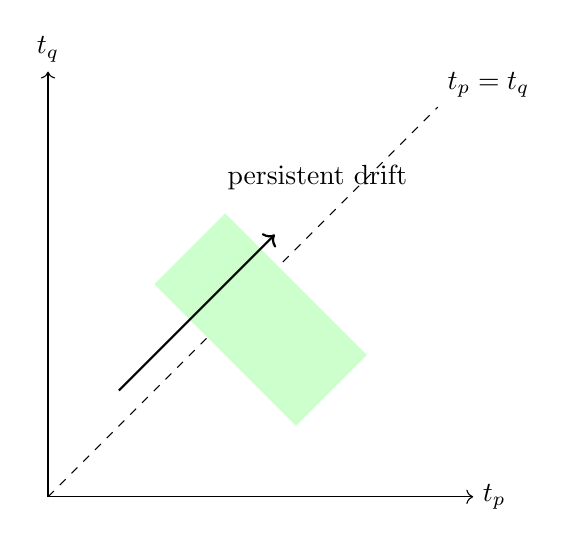
\begin{tikzpicture}[scale=0.9]

% Axes
\draw[->] (0,0) -- (6,0) node[right] {$t_p$};
\draw[->] (0,0) -- (0,6) node[above] {$t_q$};

% Diagonal
\draw[dashed] (0,0) -- (5.5,5.5) node[above right] {$t_p = t_q$};

% Drift region
\fill[green!20] (1.5,3) -- (2.5,4) -- (4.5,2) -- (3.5,1) -- cycle;

% Trajectory
\draw[thick,->] (1,1.5) -- (2,2.5) -- (3.2,3.7);

% Label
\node at (3.8,4.5) {persistent drift};

\end{tikzpicture}
\caption{Independent local time evolution allows relative timing differences
between agents to persist across interactions.}
\label{fig:persistent-drift}
\end{figure}

%---------------------------------------------------------------------------------

\subsection{Design choices and modelling rationale}
\label{subsec:ltn-design}

Local-timed negotiations combine ideas from negotiations and timed automata, but
the resulting model reflects a number of deliberate design choices.  We briefly
discuss the most important ones and contrast them with plausible alternatives.

\paragraph{Local clocks and delay vectors.}
Time elapse in LTNs is described by delay vectors $\Delta \in \Rpos^{P}$, rather
than by a single global delay.  This reflects the intended local-time semantics:
each agent progresses according to its own clock, and different agents may
accumulate time at different rates.  Using a single delay, as in timed automata,
would collapse the model back to a global-time view and eliminate the possibility
of drift between agents.

\paragraph{Reference clocks.}
Each agent $p$ is equipped with a reference clock $t_p$ that is never reset and
never appears in guards.  Reference clocks serve as a semantic device for tracking
the accumulated local time of an agent across the execution.  By excluding
reference clocks from guards, we ensure that agents cannot directly observe or
test global time; instead, comparisons between reference clocks are possible only
indirectly, via explicit synchronization.

\paragraph{Synchronization as a constraint.}
In LTNs, synchronization is expressed as the equality constraint
$t_p = t_q$ at synchronizing nodes, rather than as an instantaneous time jump or
reset.  Equality must be achieved by choosing appropriate local delays before the
action.  This makes synchronization an explicit modelling choice and separates
``time passing'' from ``time comparison'' in the semantics.

\paragraph{Node-based synchronization.}
Synchronization is associated with nodes (atomic negotiations) rather than with
outcomes.  This aligns with the interaction-centric nature of negotiations: timing
constraints are imposed at the level of joint interactions, not at the level of
local control-flow choices.

\paragraph{Local guards and resets.}
Guards and resets are local to each participating agent.  This prevents implicit
global coordination through shared clocks and ensures that all cross-agent timing
dependencies arise either from the negotiation structure itself or from explicit
synchronization nodes.

%---------------------------------------------------------------------------------

\section{Expressiveness}
\label{sec:ltn-expressiveness}

Here we understand the model better via two more examples.

\subsection{Causal Enforcement Through Synchronization}
\label{subsec:ltn-causal}

In global-time models, causality arises from control flow and shared clocks. LTNs add a new mechanism: \emph{using synchronization to force intermediate interactions}. An agent can be compelled to perform actions (accumulate local time) to align with a partner's reference clock.

\begin{example}[Forcing intermediate interactions via timing]
\label{ex:vendor}
Consider three agents: $p$, $q$, and a vendor $v$. Agent $p$ wants to ensure that $q$ has visited the vendor between their two meetings. Figure~\ref{fig:vendor} shows how this can be enforced using local clocks and synchronization.

\begin{figure}[t]
\centering
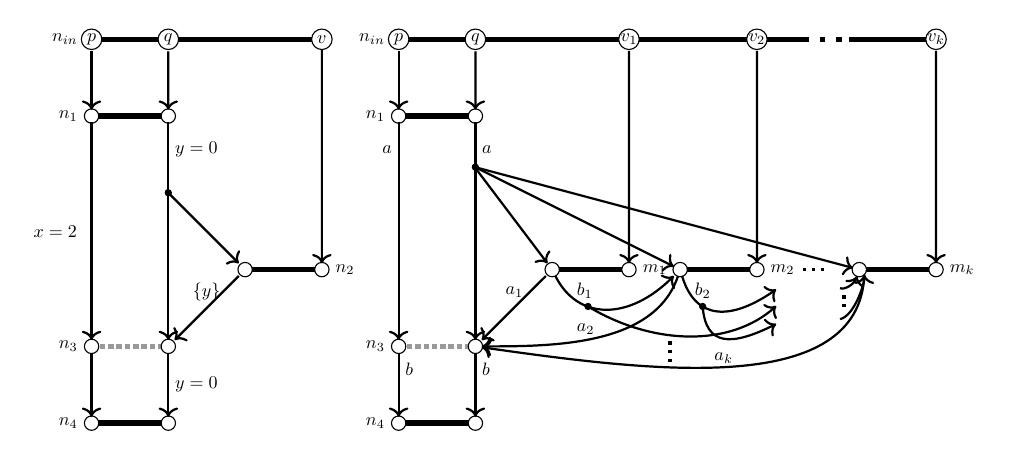
\begin{tikzpicture}[scale=0.65, every node/.style={transform shape}]

\begin{scope}[shift={(-6,0)}]
\begin{scope}[line width=2pt]
\draw (0.,0) node [left] {$n_{in}\,\,$} -- (4.5,0);
\draw (0,-1.5) node [black, left, opacity=1] {$n_1\,\,$} -- (1.5,-1.5);
\draw (3,-4.5)  -- (4.5,-4.5) node [right] {\,\,$n_2$};
\draw [densely dotted, opacity=0.4] (0,-6) node [black, left, opacity=1] {$n_3\,\,$} -- (1.5,-6);
\draw (0,-7.5) node [left] {$n_{4}\,\,$} -- (1.5,-7.5);
\end{scope}

\filldraw [fill=white]  (0,0)  circle (2mm) node 		(nip) {$p$};
\filldraw [fill=white]  (1.5,0)  circle (2mm) node 		(niq) {$q$};
\filldraw [fill=white]  (4.5,0)  circle (2mm) node 		(niv) {$v$};

\filldraw [fill=white]  (0,-1.5)  circle (1.4mm) node 	(n1p) {};
\filldraw [fill=white]  (1.5,-1.5)  circle (1.4mm) node (n1q) {};

\filldraw [fill=black]  (1.5,-3) circle (.6mm) node		(virt) {};

\filldraw [fill=white]  (3,-4.5)  circle (1.4mm) node 	(n21) {};
\filldraw [fill=white]  (4.5,-4.5)  circle (1.4mm) node (n2v) {};

\filldraw [fill=white]  (0,-6)  circle (1.4mm) node 	(n3p) {};
\filldraw [fill=white]  (1.5,-6)  circle (1.4mm) node 	(n3q) {};

\filldraw [fill=white]  (0,-7.5)  circle (1.4mm) node 	(nfp) {};
\filldraw [fill=white]  (1.5,-7.5)  circle (1.4mm) node (nfq) {};


\begin{scope}[thick,->]

\draw (nip) -- (n1p);
\draw (n1p) -- (n3p) node [midway, left, text width = 1cm] {$x=2$};
\draw (n3p) -- (nfp) node [midway, left] {};

\draw (niq) -- (n1q);
\draw (n1q) -- (n3q) node [very near start, right] {$y=0$};
\draw (virt) + (-.05,.05) -- (n21);
\draw (n21) -- (n3q) node [midway, above] {$\{y\}$};
\draw (n3q) -- (nfq) node [midway, right, text width = 1cm] {$y=0$};

\draw (niv) -- (n2v);

\end{scope}
\end{scope}

\begin{scope}[line width=2pt]
\draw (0.,0) node [left] {$n_{in}\,\,$} -- (7.9,0);
\draw (8.8,0) node [left] {} -- (10.5,0);
\draw (0,-1.5) node [black, left, opacity=1] {$n_1\,\,$} -- (1.5,-1.5);
\draw (3,-4.5)  -- (4.5,-4.5) node [right] {\,\,$m_1$};
\draw (5.5,-4.5)  -- (7,-4.5) node [right] {\,\,$m_2$};
\draw (9,-4.5)  -- (10.5,-4.5) node [right] {\,\,$m_k$};
\draw [densely dotted, opacity=0.4] (0,-6) node [black, left, opacity=1] {$n_3\,\,$} -- (1.5,-6);
\draw (0,-7.5) node [left] {$n_{4}\,\,$} -- (1.5,-7.5);
\end{scope}

\filldraw [fill=white]  (0,0)  circle (2mm) node 		(nip) {$p$};
\filldraw [fill=white]  (1.5,0)  circle (2mm) node 		(niq) {$q$};
\filldraw [fill=white]  (4.5,0)  circle (2mm) node 		(niv) {$v_1$};
\filldraw [fill=white]  (7,0)  circle (2mm) node 		(niv2) {$v_2$};
\filldraw [fill=white]  (10.5,0)  circle (2mm) node 		(nivk) {$v_k$};

\filldraw [fill=white]  (0,-1.5)  circle (1.4mm) node 	(n1p) {};
\filldraw [fill=white]  (1.5,-1.5)  circle (1.4mm) node (n1q) {};

\filldraw [fill=black]  (1.5,-2.5) circle (.6mm) node		(virt) {};

\filldraw [fill=white]  (3,-4.5)  circle (1.4mm) node 	(n21) {};
\filldraw [fill=white]  (4.5,-4.5)  circle (1.4mm) node (n2v) {};

\filldraw [fill=white]  (0,-6)  circle (1.4mm) node 	(n3p) {};
\filldraw [fill=white]  (1.5,-6)  circle (1.4mm) node 	(n3q) {};

\filldraw [fill=white]  (0,-7.5)  circle (1.4mm) node 	(nfp) {};
\filldraw [fill=white]  (1.5,-7.5)  circle (1.4mm) node (nfq) {};

\filldraw [fill=white]  (5.5,-4.5)  circle (1.4mm) node 	(v2q) {};
\filldraw [fill=white]  (7,-4.5)  circle (1.4mm) node (v2v) {};

\filldraw [white, fill=white]  (7.5,-4.8)  circle (1.4mm) node (virt2) {};
\filldraw [white, fill=white]  (8.5,-4.8)  circle (1.4mm) node (virt3) {};
\filldraw [white, fill=white]  (8.5,-5.5)  circle (1.4mm) node (virt8) {};

\filldraw [fill=black]  (3.7,-5.22)  circle (.6mm) node (virt4) {};
\filldraw [fill=black]  (5.94,-5.22)  circle (.6mm) node (virt5) {};

\filldraw [white, fill=white]  (7.5,-5.1)  circle (1.4mm) node (virt6) {};
\filldraw [white, fill=white]  (7.5,-5.5)  circle (1.4mm) node (virt7) {};

\filldraw [fill=white]  (9,-4.5)  circle (1.4mm) node 	(vkq) {};
\filldraw [fill=white]  (10.5,-4.5)  circle (1.4mm) node (vkv) {};

\begin{scope}[thick,->]

\draw (nip) -- (n1p);
\draw (n1p) -- (n3p) node [very near start, left] {$a$};
\draw (n3p) -- (nfp) node [near start, right, text width = 1cm] {$b$};

\draw (niq) -- (n1q);
\draw (n1q) -- (n3q) node [very near start, right] {$a$};
\draw (virt) + (-.05,.05) -- (n21);
\draw (n3q) -- (nfq) node [near start, right, text width = 1cm] {$b$};

\draw (niv) -- (n2v);

\draw (niv2) -- (v2v);
\draw (nivk) -- (vkv);

\draw (1.5,-2.5) -- (v2q);
\draw (1.5,-2.5) -- (vkq);

\draw (n21) -- (n3q) node [near start, left = 0cm] {$a_1$};

\end{scope}

\draw [line width=2pt, loosely dotted] (7.9,0)  -- (8.8,0) {};
\draw [very thick, dotted] (7.9,-4.5)  -- (8.4,-4.5) {};
\draw [very thick, dotted] (8.7,-5)  -- (8.7,-5.3) {};
\draw [very thick, dotted] (5.3,-5.9)  -- (5.3,-6.3) {};

\draw [thick,->] (n21) .. controls (3.5,-5.5) and(4.5,-5.5) .. (v2q) node [very near start, right = 0.1cm] {$b_1$};
\draw [thick,->] (v2q) .. controls (5.8,-5.5) and(6.5,-5.5) .. (virt2) node [very near start, right = 0cm] {$b_2$};
\draw [thick,->] (virt3) .. controls (8.7,-4.9) and (8.9,-4.8) .. (vkq);
\draw [thick,->] (virt8) .. controls (8.9,-5.4) and (9.1,-4.8) .. (9.1,-4.6);
\draw [thick,->] (v2q) .. controls (5,-6) and (3,-6) .. (n3q) node [midway, above left= -0.1cm] {$a_2$};
\draw [thick,->] (3.7,-5.22) .. controls (5,-6) and (6.5,-6) .. (virt6);
\draw [thick,->] (5.94,-5.22) .. controls (6,-6) and (6.5,-6) .. (virt7);
\draw [thick,->] (9.1,-4.6) .. controls (9,-7) and (5,-6.5) .. (n3q) node [midway, above left = -0.1cm] {$a_k$};;

\end{tikzpicture}
\caption{Vendor enforcement example. Nodes $n_1$ and $n_3$ are synchronizing (shown with dotted style). At $n_1$, outcome $a$ has guards $x = 2$ for $p$ and $y = 0$ for $q$. At $n_3$, outcome $b$ requires $y = 0$ for $q$. Synchronization forces $q$ to visit vendor $v$ at $n_2$ to accumulate the needed 2 time units. In the figure on the right, the $a$ transition has guards $x = m$ for $p$ and $y = 0$ for $q$. Each $b_i$ transition has a guard $y=1$ and a reset of $y$ to ensure exactly $1$ unit of time is spent in the nodes $m_i$ before outcomes $b_i$. The outcomes $a_i$ have a reset of $y$. The $b$ transition from $n_3$ has a guard $y=0$.}   
	\label{fig:vendor}
\end{figure}

\paragraph{Setup.} Agents $p$ and $q$ have local clocks $x$ and $y$ respectively. Nodes $n_1$ and $n_3$ are synchronizing. At $n_1$, outcome $a$ has guard $x = 2$ for $p$ and $y = 0$ for $q$.

\paragraph{What happens.} After outcome $a$ at $n_1$:
\begin{itemize}
\item Agent $p$ has advanced its reference clock by exactly 2 units (enforced by guard $x = 2$), so $t_p = 2$.
\item Agent $q$ has not advanced at all (guard $y = 0$), so $t_q = 0$.
\end{itemize}

Now both agents are ready at $n_3$ (control-flow wise), and $n_3$ is synchronizing. For outcome $b$ to occur at $n_3$:
\begin{itemize}
\item Synchronization requires $t_p = t_q$, but currently $t_p = 2$ and $t_q = 0$.
\item The guard at $b$ requires $y = 0$ for agent $q$. Since $y$ evolves with $t_q$, letting time elapse for $q$ would make $y > 0$, violating the guard.
\end{itemize}

\paragraph{The only solution.} Agent $q$ cannot simply wait—doing so would violate the guard $y = 0$. Instead, $q$ must:
\begin{enumerate}
\item Visit node $n_2$ (interaction with vendor $v$),
\item Spend exactly 2 time units there (advancing $t_q$ by 2),
\item Reset clock $y$ to zero when leaving $n_2$,
\item Return to $n_3$ with $t_q = 2$ and $y = 0$, satisfying both synchronization and the guard.
\end{enumerate}

This demonstrates \emph{causal enforcement}: the structure of timing constraints and synchronization forces $q$ to take a specific path through the negotiation. Agent $p$ can compel $q$ to perform intermediate interactions by setting up a timing mismatch that can only be resolved by those interactions.
\end{example}

\paragraph{Generalization.} This pattern extends to forcing $q$ to visit $m$ out of $k$ vendors, each requiring $1$ time unit. By setting $p$ delay to $m$ at $n_1$ and requiring $q$ to accumulate exactly $m$ time units before resynchronizing at $n_3$, we force $q$ to interact with at least $m$ vendors. This shows that LTNs can encode counting and comparison—foreshadowing undecidability.

\paragraph{Contrast with global time.} In networks of timed automata with global time, all clocks advance uniformly. One cannot create a situation where agent $p$ is "ahead" of agent $q$ in a way that forces $q$ to perform compensating actions. The local-time semantics is essential for this expressiveness.

\subsection{Non-Regular Untimed Languages}
\label{subsec:ltn-nonregular}

A fundamental result for timed automata is that their untimed languages (projecting runs onto actions, ignoring delays) are always regular. This reflects the finite-state nature of the control structure. Remarkably, LTNs can generate non-regular untimed languages.

\begin{example}[Generating $\{a^n b^n c^n \mid n \geq 0\}$]
\label{ex:anbn}
Consider the LTN in Figure~\ref{fig:abc} with two agents $p$ and $q$. Agent $p$ performs action $a$ repeatedly at node $n_1$, and agent $q$ performs action $b$ repeatedly at node $n_2$. Both can then synchronize at node $n_3$ to perform action $c$.

\begin{figure}[htb]
\centering
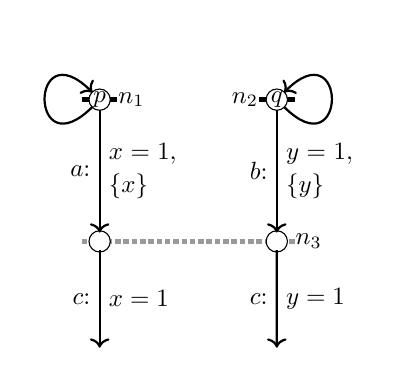
\begin{tikzpicture}[scale=0.9, every node/.style={transform shape}]

\begin{scope}[line width=2pt]
\draw (-.25,0) -- (0.25,0);
\draw (2.25,0) -- (2.75,0);
\draw [opacity=0.4, densely dotted] (-.25,-2) -- (2.75,-2);
\end{scope}

\filldraw [fill=white] (0,0) circle (1.5mm) node (pa) {$p$};
\filldraw [fill=white] (2.5,0) circle (1.5mm) node (qb) {$q$};
\filldraw [fill=white] (0,-2) circle (1.5mm) node (pc) {};
\filldraw [fill=white] (2.5,-2) circle (1.5mm) node (qc) {};

\node at (0.45,0) {$n_1$};
\node at (2.05,0) {$n_2$};
\node at (2.95,-2) {$n_3$};

\begin{scope}[thick,->]
\draw (pa) + (0,-.14) -- (pc) node [midway, left] {$a$:} node [midway, right, text width=1cm] {$x=1,$ $\{x\}$};
\draw (qb) + (0,-.14) -- (qc) node [midway, left] {$b$:} node [midway, right, text width = 1cm] {$y=1,$ $\{y\}$};
\draw (pc) -- (0,-3.5) node [midway, left] {$c$:} node [midway, right, text width=1cm] {$x=1$};
\draw (qc) -- (2.5,-3.5) node [midway, left] {$c$:} node [midway, right, text width=1cm] {$y=1$};
\draw (-0.1,-0.1) .. controls (-1,-1) and (-1,1) .. (-0.1,0.1);
\draw (2.6,-0.1) .. controls (3.5,-1) and (3.5,1) .. (2.6,0.1);
\end{scope}

\end{tikzpicture}
\caption{Non-regular untimed language. Each loop iteration of $a$ and $b$ takes exactly 1 time unit. Node $n_3$ is synchronizing with guards $x = 1$ and $y = 1$. This forces the number of $a$s to equal the number of $b$s before $c$ occurs.}
\label{fig:abc}
\end{figure}

\paragraph{Mechanism.} Both $p$ and $q$ start with reference clocks at zero. Each iteration of $a$ at $n_1$ takes exactly 1 time unit (guard $x = 1$, then reset $x$), advancing $t_p$ by 1. Similarly, each $b$ at $n_2$ advances $t_q$ by 1. The loops are concurrent—there's no ordering between $a$s and $b$s.

Node $n_3$ is synchronizing and requires:
\begin{itemize}
\item $t_p = t_q$ (synchronization condition),
\item $x = 1$ and $y = 1$ (guards at outcome $c$).
\end{itemize}

For these conditions to hold simultaneously:
\begin{itemize}
\item Both agents must have performed their last loop iteration exactly 1 time unit ago,
\item Both agents must have performed the same number of loop iterations (so $t_p = t_q$).
\end{itemize}

Therefore, if $p$ performs $n$ iterations of $a$ and $q$ performs $m$ iterations of $b$, action $c$ can occur if and only if $n = m$. The untimed language includes all words of the form $w \cdot c$ where $w$ has equal number of $a$ and $b$. Note that we can add another identical process with identical guards and which also time-synchronizes at $n_3$, and then the language would be beyond context-free.
\end{example}

\paragraph{Why this matters.} This demonstrates that:
\begin{enumerate}
\item LTNs can encode \emph{counting} constraints across concurrent actions,
\item Synchronization acts as a \emph{comparison} operator between accumulated counts (via reference clocks),
\item The untimed behavior transcends finite-state structure—language-theoretically, LTNs are more powerful than timed automata.
\end{enumerate}

\begin{table}[t]
\centering
\begin{tabular}{ll}
\hline
\textbf{Feature} & \textbf{Enables} \\
\hline
Local delays & Independent progress and drift \\
Reference clocks & Persistent timing information across interactions \\
Synchronizing nodes & Comparison of accumulated drift \\
Unsynchronized nodes & Unbounded drift accumulation \\
Guards and resets & Counter-style encodings via timing constraints \\
\hline
\end{tabular}
\caption{Sources of expressiveness in local-timed negotiations.}
\label{tab:ltn-expressiveness}
\end{table}

This expressiveness enables rich modelling but also implies undecidability, as we'll see next.

%---------------------------------------------------------------------------------
\begin{figure}[t]
\centering
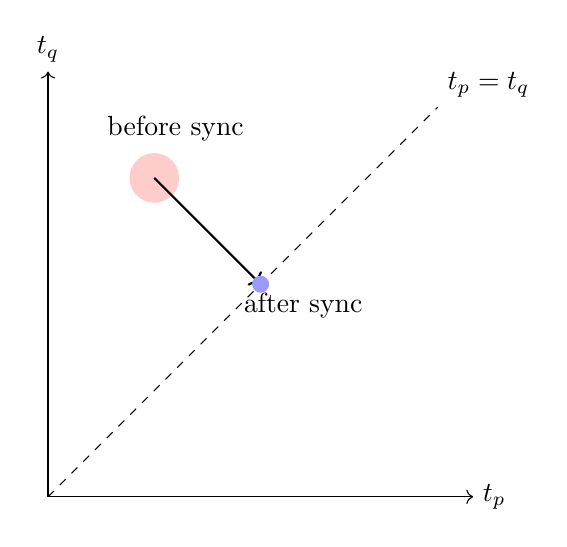
\begin{tikzpicture}[scale=0.9]

% Axes
\draw[->] (0,0) -- (6,0) node[right] {$t_p$};
\draw[->] (0,0) -- (0,6) node[above] {$t_q$};

% Diagonal
\draw[dashed] (0,0) -- (5.5,5.5) node[above right] {$t_p = t_q$};

% Pre-synchronization region
\fill[red!20] (1.5,4.5) circle (0.35);
\node at (1.8,5.2) {before sync};

% Arrow to diagonal
\draw[thick,->] (1.5,4.5) -- (3,3);

% Post-synchronization point
\fill[blue!40] (3,3) circle (0.12);
\node at (3.6,2.7) {after sync};

\end{tikzpicture}
\caption{A time-synchronizing interaction collapses relative timing differences,
allowing accumulated information to be compared or reset.}
\label{fig:selective-sync}
\end{figure}

\section{Undecidability of reachability}
\label{sec:ltn-undec}

\paragraph{Proof roadmap.}
The undecidability proof proceeds by a reduction from the halting problem of
$2$-counter machines.  The key idea is to encode counter values as differences
between reference clocks of carefully chosen agents.

Increment and decrement operations are implemented by allowing certain agents to
accumulate local time while others are forced to remain idle.  Zero-tests rely on
synchronizing nodes, which require equality of reference clocks and thus permit
the comparison of accumulated drift.  Unsynchronized nodes are essential for
allowing drift to grow without bound, while synchronized nodes are essential for
testing and transferring this information.

The construction alternates systematically between synchronized and
unsynchronized phases.  This interplay is what enables the simulation of
unbounded counters and ultimately yields undecidability of
location-reachability.

We now show that location-reachability for LTNs is undecidable.  The proof reduces
the halting problem of $2$-counter machines to reachability in an LTN.  The key
source of power is the unbounded drift between reference clocks of different agents,
together with the ability to impose synchronization at selected nodes.

\begin{theorem}
\label{thm:undecidability}
Location-reachability is undecidable for local-timed negotiations.
\end{theorem}

The rest of the section is devoted to proving
Theorem~\ref{thm:undecidability}. We will encode the halting problem
of a $2$-counter machine as the reachability problem for a local-timed
negotiation.

\subsection{Two-counter machines}
\label{subsec:2cm}

\noindent \emph{Counter machines.} A $2$-counter machine $M$ is a program that manipulates two counters, $C_1$ and $C_2$,
each of which can hold a non-negative number. The machine is given as
a sequence of labelled instructions $\ell:I$, where $I$ is one of the following for some $i \in \{1, 2\}$: 
\begin{description}
\item[increment] $C_i + +$, which increments the value of the
  counter $C_i$ and goes to the next instruction
  $\ell+1$.
\item[decrement] if $C_i>0$ then $C_i- -$, which decrements $C_i$ and continues with the next instruction
  $\ell+1$. If the value of $C_i$ is $0$, then the program is blocked. 
\item[jump-on-zero] if $C_i= = 0$ goto $\ell'$, which transfers control to the instruction labelled $\ell'$ if counter $C_i$ is $0$ for
  $i\in\{1,2\}$. If $C_i>0$, it continues to the instruction $\ell+1$.
\end{description}
The counter machine is said to halt if it reaches the final
instruction. A configuration of $M$ is a triple $(\ell, c_1, c_2)$ representing the current instruction $\ell$ that needs to be executed and the current values $c_1, c_2 \ge 0$ of the counters $C_1, C_2$ respectively. The transitions $(\ell, c_1, c_2) \xra{} (\ell', c'_1, c'_2)$ follow naturally from the description above.

\subsection{Overview of the reduction}
\label{subsec:red-overview}

The negotiation $\Nn_M$ that we
construct will have $6$ agents $p_1, q_1, r_1, p_2, q_2, r_2$. Agents
$p_1, q_1, r_1$ simulate counter $C_1$, and the rest simulate
$C_2$. Let $i \in \{1, 2\}$. The local clocks of $p_i, q_i, r_i$ are
respectively $\{x_{p_i}\}$, $\{x_{q_i}, x'_{q_i}\}$ and $\{x_{r_i}\}$. Additionally, we have the reference clocks $t_\a$ for each agent $\a$. For every instruction $\ell$, we will have a node
$n_\ell$ in which all the six agents participate.
A configuration $(C, v)$ of $\Nn_M$ is said to encode configuration
$(\ell, c_1, c_2)$ of $M$ if:
\begin{itemize}
\item $C(\a) = \{n_\ell\}$ for every agent $\a$,
\item $v(x) = 0$ for all local clocks (and reference clocks can take any value),
\item $v(t_{r_1}) \le v(t_{q_1}) \le v(t_{p_1})$ and $v(t_{r_2}) \le v(t_{q_2}) \le v(t_{p_2})$, and 
\item $v(t_{p_1} - t_{q_1}) = c_1$ and $v(t_{p_2} - t_{q_2}) = c_2$,
\end{itemize}
The initial configuration of $\Nn_M$ has every agent in $n_{\ell_0}$, where $\ell_0$ is the first instruction in $M$ and every clock (including reference clocks) to be $0$. Since reference clocks are never reset and only increase through delay
steps, differences between reference clocks are preserved unless
explicitly modified by controlled delay.

We will have a gadget in $\Nn_M$ corresponding to each instruction in the counter machine. Let $(C, v), (C',v')$ be configurations that encode $(\ell, c_1, c_2)$ and $(\ell', c'_1, c'_2)$ respectively. A run $(C, v) \xra{} \cdots \xra{} (C', v')$ such that none of the intermediate configurations encodes any counter machine configuration will be called a \emph{big step}. We denote a big step as $(C, v) \Rightarrow (C', v')$. Our gadgets will ensure the following two properties.
\begin{itemize}
\item Let $(\ell, c_1, c_2) \xra{} (\ell', c'_1, c'_2)$ in $M$. Then from every configuration $(C, v)$ that encodes $(\ell, c_1, c_2)$, there is a big step $(C, v) \Rightarrow (C', v')$ to some configuration $(C', v')$ that encodes $(\ell', c'_1, c'_2)$.
\item Let $(C, v), (C', v')$ be arbitrary configurations of $\Nn_M$ that encode $(\ell, c_1, c_2)$ and $(\ell', c'_1, c'_2)$ respectively. If $(C, v) \Rightarrow (C', v')$ is a big step, then $(\ell, c_1, c_2) \xra{} (\ell', c'_1, c'_2)$ in $M$.
\end{itemize}
The first property ensures that for every path $(\ell^0, c^0_1, c^0_2)
\xra{} (\ell^1, c^1_1, c^1_2) \xra{} \cdots$, there is a sequence of
big steps $(C_0, v_0) \Rightarrow (C_1, v_1) \Rightarrow \cdots$ such
that  $(C_i, v_i)$ encodes $(\ell^i, c^i_1, c^i_2)$. The second
property ensures the reverse: from a sequence of big steps, we get
a corresponding run in counter machine. We will now describe each
gadget and show that the two properties are satisfied.  

Throughout the gadgets, guards of the form $x=0$ ensure that no agent can
let time elapse before executing the corresponding action; any positive
delay would violate the guard and block the run.

\subsection{Instruction gadgets}
\label{subsec:gadgets}

\begin{figure}[t]
\begin{center}
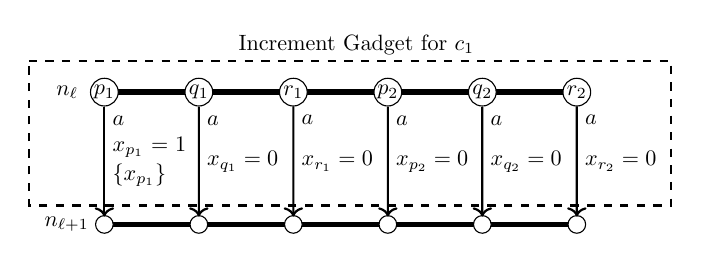
\begin{tikzpicture}[scale=0.8, every node/.style={transform shape}]

\begin{scope}[line width=2pt]
\draw (0,0) -- (7.5,0);
\draw (0,-2.1) -- (7.5,-2.1);
\end{scope}

\filldraw [fill=white]  (0,0)	  circle (2.2mm) node (nip1) [label={left:$n_{\ell}$}] {$p_1$};
\filldraw [fill=white]  (1.5,0)	  circle (2.2mm) node (niq1) {$q_1$};
\filldraw [fill=white]  (3,0)	  circle (2.2mm) node (nir1) {$r_1$};
\filldraw [fill=white]  (4.5,0)	  circle (2.2mm) node (nip2) {$p_2$};
\filldraw [fill=white]  (6,0)	  circle (2.2mm) node (niq2) {$q_2$};
\filldraw [fill=white]  (7.5,0)	  circle (2.2mm) node (nir2) {$r_2$};
\filldraw [fill=white]  (0,-2.1)	  circle (1.4mm) node (n2p1) [label={left:$n_{\ell + 1}$}] {};
\filldraw [fill=white]  (1.5,-2.1)	  circle (1.4mm) node (n2q1) {};
\filldraw [fill=white]  (3,-2.1)	  circle (1.4mm) node (n2r1) {};
\filldraw [fill=white]  (4.5,-2.1)	  circle (1.4mm) node (n2p2) {};
\filldraw [fill=white]  (6,-2.1)	  circle (1.4mm) node (n2q2) {};
\filldraw [fill=white]  (7.5,-2.1)	  circle (1.4mm) node (n2r2) {};

\begin{scope}[thick,->]
  \draw (nip1) -- node [very near start, right] {$a$} (n2p1)	 node [midway,right, text width=1.25cm] {$x_{p_1}=1$ $\{x_{p_1}\}$};
  \draw (niq1) -- node [very near start, right] {$a$} (n2q1)	 node [midway,right, text width=1.25cm] {$x_{q_1}=0$};
  \draw (nir1) -- node [very near start, right] {$a$} (n2r1)	 node [midway,right, text width=1.25cm] {$x_{r_1}=0$};
  \draw (nip2) -- node [very near start, right] {$a$} (n2p2)	 node [midway,right, text width=1.25cm] {$x_{p_2}=0$};
  \draw (niq2) -- node [very near start, right] {$a$} (n2q2)	 node [midway,right, text width=1.25cm] {$x_{q_2}=0$};
  \draw (nir2) -- node [very near start, right] {$a$} (n2r2)	 node [midway,right, text width=1.25cm] {$x_{r_2}=0$};
\end{scope}

\draw [dashed, thick] (-1.2,0.5) -- (9,0.5) -- (9,-1.8) -- (-1.2,-1.8) -- (-1.2,0.5);

\node at (4,.75) {Increment Gadget for $c_1$};
\end{tikzpicture}
\caption{Gadget for implementing increment instruction on $c_1$}
\label{fig:increment}
\end{center}
\end{figure}


\noindent \emph{Increment.} Assume an instruction $\ell: C_1 ++$ with $\ell$ not being the final instruction. The case with $C_2++$ is symmetric. Every configuration $(\ell, c_1, c_2)$ on executing this instruction goes to $(\ell + 1, c_1 + 1, c_2)$. Figure~\ref{fig:increment} shows the gadget for the increment instruction. All agents other than $p_1$ cannot elapse time due to the guard checking local clocks to $0$. Agent $p_1$ elapses
exactly one time unit, after which clock $x_{p_1}$ is reset.
It is easy to see that the configuration $(C', v')$ that results from $(C, v)$
encodes $(\ell', c_1 + 1, c_2)$. The big step $(C, v) \Rightarrow (C',v')$ is in fact a single transition. Both the properties are easily seen to be satisfied. 

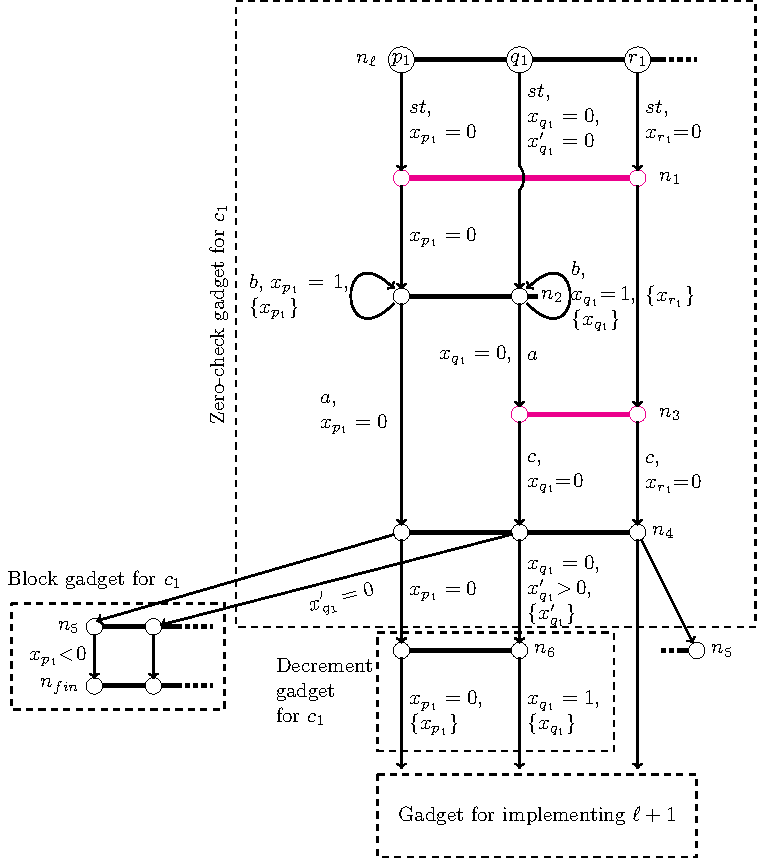
\includegraphics{decrement-gadget.pdf}

\paragraph*{Decrement.} Consider a decrement instruction: if $C_1 > 0$
then $C_1 --$. We have
$(\ell, c_1, c_2) \xra{} (\ell+1, c_1 - 1, c_2)$ if $c_1 > 0$. The
first task is to check if $c_1 > 0$. Recall that in the negotiation the difference $t_{p_1} - t_{q_1}$ gives the value of $c_1$. Our idea is to let $q_1$ elapse time to
synchronize with $p_1$ and check if this time elapse needed for
synchronization is strictly above $0$ or not. However, in this
process, we lose the actual value of the counter. In order to maintain the same difference between $t_{p_1}$ and $t_{q_1}$, we make use of the auxiliary process $r_1$.

Consider a configuration $(C, v)$ that encodes $(\ell, c_1, c_2)$. By our definition, $v(t_{r_1}) \le v(t_{p_1})$ and $v(t_{p_1} - t_{q_1}) = c_1$. 
\begin{itemize}
 
\item We first let $r_1$ synchronize with $p_1$, while $p_1$
  elapses no time.
\item Next, we keep moving both $p_1$ and $q_1$ by $1$ unit each until
  $q_1$ synchronizes with $r_1$. In this entire process $r_1$ is not
  allowed to elapse time.
\end{itemize}
By the end of this, we will get a valuation $v'$ with the same difference $v'(t_{p_1} - t_{q_1}) = c_1$
since both the agents were moved by the same amount. Moreover, we can
use an additional clock to check whether in the process of $q_1$
synchronizing with $r_1$, a non-zero time had elapsed in $q_1$.

The gadget is depicted in Figure~\ref{fig:jump-decrement}. For simplicity, we do not index the intermediate nodes $n_1, n_2, n_3, n_4$ by $\ell$. The computation proceeds in three phases. Below, we show the run of $\Nn_M$ along this gadget, restricted to the agents $p_1, q_1, r_1$. The other three agents simply move to the next possible instruction (this is not shown in the figure for simplicity). 

\smallskip

\noindent \emph{Phase 1.} Synchronize $r_1$ with $p_1$ maintaining no time
elapse in $p_1$ as follows: $((n_\ell, n_\ell, n_\ell), v) \xra{}
((n_1, n_2, n_1), v_1) \xra{} ((n_2, n_2, n_3), v_3)$. After the last
action, agents $p_1$ and $r_1$ are synchronized, that is,
$v_3(t_{p_1}) = v_3(t_{r_1})$. This is due to the node $n_1$ being a
synchronization node. Moreover, $v_3(t_{p_1}) = v(t_{p_1})$, due to
the guard $x_{p_1} = 0$. Similarly, $v_3(t_{q_1}) = v(t_{q_1})$ due to
$x_{q_1} = 0$.

\smallskip

\noindent \emph{Phase 2.} Move $p_1$ and $q_1$ repeatedly by one unit each:  $((n_2, n_2, n_3), v_3) \xra{b} ((n_2, n_2, n_3), v_3^1) \xra{b} \cdots \xra{b} ((n_2, n_2, n_3), v_3^k)$. By the end of $k$ iterations of $b$, we have $v^k_3(t_{p_1}) = v(t_{p_1}) + k$ and $v^k_3(t_{q_1}) = v(t_{q_1}) + k$.

\smallskip

\noindent \emph{Phase 3.} Check if the reference clocks of $q_1$ and $r_1$
are equal: $((n_2, n_2, n_3), v_3^k)$
$\xra{a} ((n_4, n_3, n_3), v_4) \xra{c} ((n_4, n_4, n_4), v_5)$. The
outcome $c$ at $n_4$ can be fired only if the reference clocks of
$q_1$ and $r_1$ are equal: that is, $v_4(t_{q_1}) = v_4(t_{r_1})$. Due
to the guard checking for $0$ at $a$ and $c$, we have
$v_5(t_{q_1}) = v_4(t_{q_1}) = v_3^k(t_{q_1})$. From Phase 2, this
value equals $v(t_{q_1}) + k$. Secondly, notice that
$v_4(t_{r_1}) = v_3(t_{r_1})$, which from Phase 1 equals
$v(t_{p_1})$. From the equality $v_4(t_{q_1}) = v_4(t_{r_1})$, we get
$v(t_{q_1}) + k = v(t_{p_1})$.  This shows that
$k = v(t_{p_1}) - v({t_{q_1}})$. The number of times the loop $b$ is
done equals the difference between $t_{p_1}$ and $t_{q_1}$ at the
start of this gadget. If the number of $b$ iterations is more than
this value or less than this value, location $(n_3, c)$ cannot be
executed and the negotiation cannot proceed further. At the end of the gadget, the ordering
$v(t_{r_1}) \le v(t_{q_1}) \le v(t_{p_1})$ is restored, ensuring that
subsequent gadgets operate under the same encoding invariant.


When action $c$ is done, the clock $x'_{q_1}$ holds the time between
$st$ and $c$ for agent $q_1$, and this is exactly $k$. If $k > 0$ the
value of $t_{q_1}$ is increased by $1$, resulting in the counter value
getting decremented and the agents move to the next instruction (shown
as the decrement gadget in the figure). Otherwise, the agents are sent
to a gadget from which there is no run (shown as the block gadget in
the figure).
Notice the interplay between synchronized and unsynchronized nodes in
this gadget. It is crucial that $n_2$ is unsynchronized, whereas
nodes $n_1, n_3$ need to be.
Note that after Phase~1 the value of $t_{r_1}$ remains fixed throughout
Phase~2, while each execution of $b$ strictly increases $t_{q_1}$.
Hence, once $t_{q_1} > t_{r_1}$, equality can never be restored, and the
final synchronization test necessarily fails.

%diagram for intuition

\paragraph{Concrete example.}
We illustrate the decrement gadget with a concrete example.  Consider a
configuration $(C,v)$ encoding $(\ell,c_1,c_2)$ with $c_1=2$, so that
$v(t_{p_1}) - v(t_{q_1}) = 2$ and all local clocks are $0$.

\emph{Positive case ($c_1>0$).}
In Phase~1, agent $r_1$ synchronizes with $p_1$ without any time elapse in $p_1$,
so after synchronization we have
$v(t_{r_1}) = v(t_{p_1})$ and still $v(t_{p_1}) - v(t_{q_1}) = 2$.
In Phase~2, the loop labeled $b$ is executed twice, advancing both $p_1$ and
$q_1$ by one unit each time.  After two iterations, $q_1$ reaches the same
reference time as $r_1$, and synchronization at the next node becomes possible.
Since a positive amount of time has elapsed in this phase, the gadget proceeds
to the decrement branch, reducing the encoded counter value from $2$ to $1$.

\emph{Zero case ($c_1=0$).}
Now suppose $(C,v)$ encodes $c_1=0$, so that
$v(t_{p_1}) = v(t_{q_1})$ initially.  Phase~1 again synchronizes $r_1$ with
$p_1$.  In Phase~2, the loop $b$ cannot be executed even once: advancing $q_1$
would immediately make its reference clock larger than that of $r_1$, and the
final synchronization test would fail.  Consequently, no run can reach the
decrement branch, and the execution is forced into the blocking gadget.

This example shows how the feasibility of synchronization distinguishes the
cases $c_1>0$ and $c_1=0$ without directly testing the counter value.

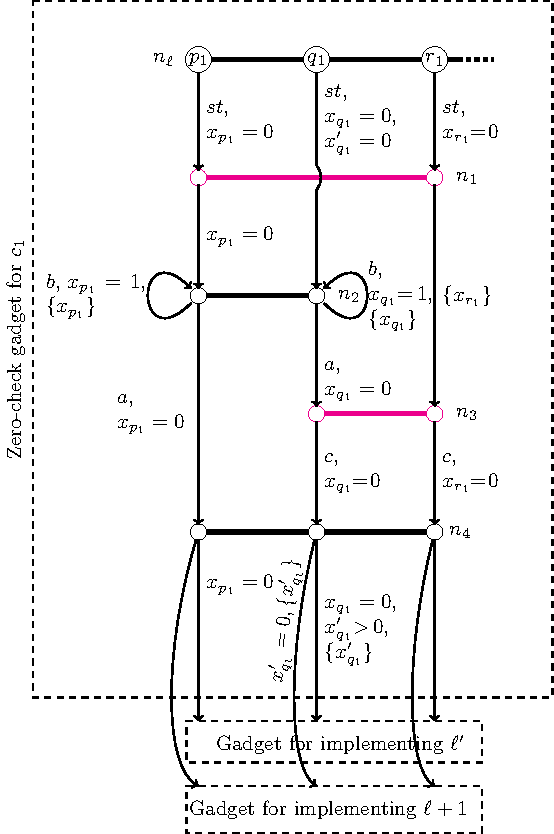
\includegraphics{jump-gadget.pdf}

\noindent \emph{Jump-on-zero.} This gadget is similar to the decrement
gadget, where the first part was to check if $C_1$ is $0$ or not. When $C_1 == 0$, the gadget jumps to the
relevant instruction, otherwise it moves to the next instruction in
sequence. The gadget is shown in~\cite{mukund2023localtime}. 

%---------------------------------------------------------------------------------
\section{Summary and perspective}
\label{sec:summary-ch3}

This chapter introduced \emph{local-timed negotiations} (LTNs) as a real-time
extension of negotiations in which each agent carries its own set of local clocks,
and time elapses \emph{locally} (via delay vectors).  The semantics combines three
ingredients:

\begin{itemize}
  \item the negotiation-style control flow captured by markings (who is ready to
        participate in which node),
  \item local clock constraints (guards and resets attached to outcomes), and
  \item \emph{optional} explicit synchronization at selected nodes, expressed as the
        constraint that all participating agents have equal reference clocks.
\end{itemize}

We illustrated how LTNs model timing constraints between interactions using the
ATM example (Figure~\ref{fig:ATM}).  We then highlighted two expressiveness
phenomena that are characteristic of the local-time setting:
(i) synchronization can be used as a \emph{causal enforcement} mechanism, forcing
agents to perform intermediate interactions (Section~\ref{subsec:ltn-vendor}),
and (ii) the untimed outcome language of an LTN can be non-regular
(Section~\ref{subsec:ltn-nonregular}), in sharp contrast to timed automata where
the untimed language is always regular.

The main algorithmic message of the chapter is negative: we proved that
\emph{location-reachability is undecidable} for LTNs (Theorem~\ref{thm:undecidability})
by a reduction from halting of $2$-counter machines.  Conceptually, the reduction
pinpoints the source of power: reference clocks can drift arbitrarily, and
synchronizing nodes allow the system to \emph{compare} and \emph{transfer}
information encoded in those drifts.  In particular, the proof relies on a careful
interplay between synchronized nodes (where equality of reference clocks must be
met) and unsynchronized nodes (where agents can advance independently and thus
accumulate drift).

\smallskip
\noindent\textbf{Perspective.}
LTNs sit between two well-studied extremes.  On one hand, they inherit the
interaction-centric, partial-order flavour of negotiations; on the other hand,
they adopt a clock-based view of time as in timed automata, but without a global
time line.  This combination is expressive enough to model realistic timing
patterns (local deadlines, response windows, and time-bounded protocols), while
also making plain that \emph{unrestricted} local-time drift together with
\emph{explicit} synchronization yields a model beyond decidability for basic
reachability.

This motivates the rest of the thesis: to identify robust restrictions that
preserve the modelling advantages of LTNs but regain algorithmic tractability.
Two orthogonal axes stand out naturally from this chapter:
\begin{itemize}
  \item restricting (or eliminating) explicit synchronization, so that drift cannot
        be tested directly; and
  \item bounding the amount of drift that can accumulate (globally, per-agent, or
        per-cycle), so that comparisons do not simulate unbounded counters.
\end{itemize}
Understanding where decidability reappears along these axes also clarifies which
expressiveness features (e.g.\ enforcing intermediate interactions, or generating
non-regular untimed languages) survive in the restricted models, and which do not.

\smallskip
\paragraph{What causes undecidability?} The reduction pinpoints two features:
\begin{enumerate}
\item \textbf{Unbounded drift}: Reference clocks can diverge arbitrarily, encoding unbounded integer values (counter contents).
\item \textbf{Explicit synchronization}: Synchronizing nodes allow the system to test equality of reference clocks, enabling comparisons and conditional behavior based on encoded values.
\end{enumerate}

Removing or restricting either feature may recover decidability—this is the focus of Part~II.

%---------------------------------------------------------------------------------
\section{Coming next}
\label{sec:next-ch3}

This chapter concludes Part~I, where we introduced local-timed negotiations and
established that, in their full generality, even basic location-reachability is
undecidable (Theorem~\ref{thm:undecidability}).  The remainder of the thesis
(Part~II) is devoted to recovering decidability by identifying restrictions that
preserve the modelling advantages of LTNs while taming the two sources of
algorithmic hardness exposed by the reduction: \emph{unrestricted drift} between
local reference clocks and the ability to \emph{test} that drift via explicit
synchronization.

Part~II develops several decidable fragments along complementary axes:
\begin{itemize}
  \item \textbf{Extreme synchronization regimes:} we study the two endpoints where
        synchronization is either \emph{forbidden} (synchronization-free LTNs) or
        \emph{mandatory} at every interaction (always-synchronized LTNs), and
        analyze how these extremes change both expressiveness and the reachability
        problem.
  \item \textbf{Quantitative restrictions on drift:} we introduce drift-bounded
        variants that limit how far apart agents' reference clocks may deviate,
        yielding finite (or well-structured) symbolic state spaces.
  \item \textbf{Structural restrictions:} we consider communication/topological
        constraints on the underlying negotiation graph---for instance, connected
        communication patterns---and show how they can re-establish decidability
        even when clocks remain local.
  \item \textbf{Few-process settings:} we isolate the two-process case as a
        particularly informative boundary, where local time still matters but the
        concurrency structure becomes constrained enough to admit specialized
        algorithms.
\end{itemize}

\smallskip
\noindent\textbf{Immediate next chapter.}
We begin Part~II by focusing on the first axis above, namely the two extreme
synchronization regimes: \emph{synchronization-free} LTNs and \emph{always-synchronized}
LTNs.


\part{Decidable subclasses for reachability in LTNs}

Part~I established local-timed negotiations as a model for concurrent real-time systems and showed that this expressiveness comes at a fundamental cost: location reachability is undecidable in the presence of unrestricted local-time drift combined with selective synchronization (Chapter~\ref{chap:ltn}). The undecidability proof isolated two sources of algorithmic hardness—unbounded divergence of reference clocks and the ability to compare accumulated drift via synchronizing nodes.

In this part, we turn to the complementary question: under which restrictions can reachability be recovered as a decidable problem, without collapsing the model back to global time or eliminating concurrency altogether? We study several fragments of local-timed negotiations obtained by constraining synchronization patterns, temporal drift, or communication structure, and develop tailored proof techniques for each. Chapter~\ref{chap:fragments} begins this investigation by analyzing the two extreme synchronization regimes, which serve as conceptual and technical anchor points for the decidable landscape explored in the chapters that follow.

%%__________________________________________________________________________________

\chapter{Synchronization Extremes: Free and Always-Synchronizing LTNs}
\label{chap:fragments}

Chapter~\ref{chap:ltn} showed that location reachability is undecidable for general
local-timed negotiations. The proof of Theorem~\ref{thm:undecidability} identified
two features whose interaction is essential for this result:

\begin{enumerate}
\item \emph{Unbounded clock drift}: the reference clocks $t_p$ and $t_q$ of different
agents may diverge arbitrarily, allowing the encoding of unbounded integer values.
\item \emph{Explicit synchronization}: synchronizing nodes require equality of
reference clocks, enabling the system to compare and condition behavior on
accumulated drift.
\end{enumerate}

It is precisely the combination of these two mechanisms—arbitrary accumulation
of drift and the ability to test it—that yields the expressive power of counter
machines. Part~II explores how decidability can be recovered by restricting one
or both of these sources of power.

This chapter focuses on the first axis of restriction, namely synchronization.
Rather than allowing arbitrary mixtures of synchronizing and non-synchronizing
nodes, we study the two extreme regimes:
\begin{itemize}
\item \textbf{Synchronization-free LTNs} ($\text{Sync} = \emptyset$), where no node
imposes equality of reference clocks and agents evolve completely independently.
\item \textbf{Always-synchronizing LTNs} ($\text{Sync} = N$), where every interaction
requires temporal alignment of participating agents.
\end{itemize}

In both cases, the critical interaction between unbounded drift and synchronization
is eliminated, albeit in opposite ways. As a consequence, location reachability
becomes decidable.

\paragraph{Conceptual role of the extremes.}
In these two fragments, we recover decidability by removing the interplay between drift and synchronization. Understanding why these extremes are decidable clarifies which features cause undecidability in the general model.
Despite of having the same worst-case complexity, the two fragments require
fundamentally different proof techniques. Synchronization-free LTNs admit a
componentwise abstraction that exploits the complete independence of agents,
whereas always-synchronizing LTNs collapse to a global-time semantics and can be
reduced to classical timed automata.

\paragraph{Main results.}
The central results of this chapter are the following.

\begin{theorem}[Chapter results]
\label{thm:chapter-results}
Location reachability is PSPACE-complete for each of the following classes:
\begin{enumerate}
\item synchronization-free local-timed negotiations (Section~\ref{sec:syncfree});
\item always-synchronizing local-timed negotiations (Section~\ref{sec:always-sync}).
\end{enumerate}
\end{theorem}

In both cases, the complexity matches that of reachability for timed automata.
Thus, while these fragments do not exploit the negotiation structure to reduce
complexity, they also do not incur additional algorithmic cost beyond what is
inherent to quantitative timing.

\paragraph{Organization.}
Section~\ref{sec:syncfree} studies synchronization-free LTNs via a product-style
region abstraction. Section~\ref{sec:always-sync} analyzes always-synchronizing
LTNs by reducing them to a global-time model. Section~\ref{sec:fragments-synthesis}
synthesizes the lessons from both extremes, and Section~\ref{sec:fragments-next}
positions them within the broader landscape of decidable fragments studied in
subsequent chapters.

%__________________________________________________________________________________
%%%%%%%%%%%%%%%%%%%%%%%%%%%%%%%%%%%%%%%%%%%%%%%%%%%
\begin{comment}
\section{A Running Example}
\paragraph{A running example.}
The following simple two-agent LTN will be used to illustrate the proof techniques for synchronization-free and always-synchronizing LTNs.

Let $P = \{p,q\}$. Each agent has one local clock:
$X_p = \{x\}$ and $X_q = \{y\}$.
The negotiation has three nodes: $N = \{n_0, n_1, n_2\}$
with domains: $\text{dom}(n_0) = \{p,q\}, 
\text{dom}(n_1) = \{p\}, 
\text{dom}(n_2) = \{p,q\}.$

\begin{figure}[t]
\centering

% --- Diagram 1: Synchronization-Free Semantics ---
\begin{subfigure}[b]{0.45\textwidth}
\centering
\resizebox{\textwidth}{!}{%
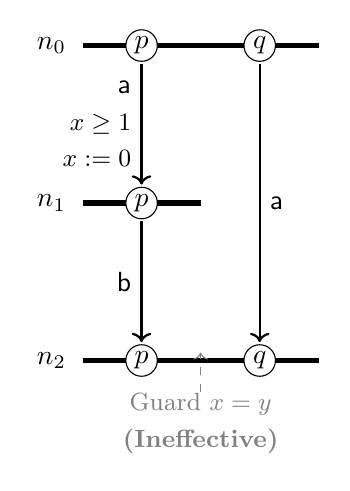
\begin{tikzpicture}
    % Nodes (Bars)
    \draw[line width=2pt] (0,4) node[left] {$n_0\,$} -- (3,4);
    \draw[line width=2pt] (0,2) node[left] {$n_1\,$} -- (1.5,2);
    \draw[line width=2pt] (0,0) node[left] {$n_2\,$} -- (3,0);

    % Ports
    \filldraw[fill=white] (0.75,4) circle (2mm) node (p_n0) {$p$};
    \filldraw[fill=white] (2.25,4) circle (2mm) node (q_n0) {$q$};
    
    \filldraw[fill=white] (0.75,2) circle (2mm) node (p_n1) {$p$};
    
    \filldraw[fill=white] (0.75,0) circle (2mm) node (p_n2) {$p$};
    \filldraw[fill=white] (2.25,0) circle (2mm) node (q_n2) {$q$};

    % Edges
    % p: n0 -> n1
    \draw[->, thick] (p_n0) -- (p_n1) node[midway, left, align=right] {$\mathsf{a}$ \\ \small $x \ge 1$ \\ \small $x:=0$};
    
    % q: n0 -> n2 (Wait)
    \draw[->, thick] (q_n0) -- (q_n2) node[midway, right] {$\mathsf{a}$};

    % p: n1 -> n2
    \draw[->, thick] (p_n1) -- (p_n2) node[midway, left] {$\mathsf{b}$};

    % Guard visualization
    \node[text=gray, align=center] at (1.5, -0.8) {\small Guard $x=y$ \\ \small \textbf{(Ineffective)}};
    \draw[->, gray, dashed] (1.5, -0.4) -- (1.5, 0.1);
\end{tikzpicture}
}
\caption{\textbf{Synchronization-Free.} Agent $q$ waits while $p$ executes $n_1$. Since $n_2$ does not synchronize clocks, the local clocks $x$ and $y$ drift apart, making the equality check $x=y$ ineffective (semantics ignore it).}
\label{fig:ltn_sync_free}
\end{subfigure}
\hfill
% --- Diagram 2: Always-Synchronizing Semantics ---
\begin{subfigure}[b]{0.45\textwidth}
\centering
\resizebox{\textwidth}{!}{%
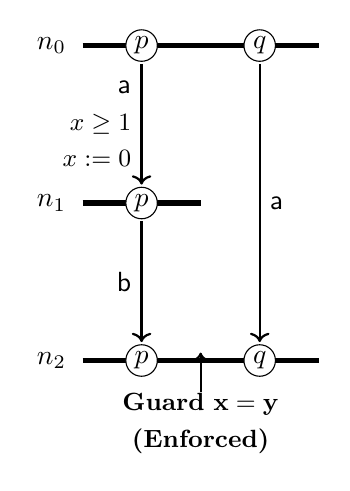
\begin{tikzpicture}
    % Nodes (Bars)
    \draw[line width=2pt] (0,4) node[left] {$n_0\,$} -- (3,4);
    \draw[line width=2pt] (0,2) node[left] {$n_1\,$} -- (1.5,2);
    \draw[line width=2pt] (0,0) node[left] {$n_2\,$} -- (3,0);

    % Ports
    \filldraw[fill=white] (0.75,4) circle (2mm) node (p_n0) {$p$};
    \filldraw[fill=white] (2.25,4) circle (2mm) node (q_n0) {$q$};
    
    \filldraw[fill=white] (0.75,2) circle (2mm) node (p_n1) {$p$};
    
    \filldraw[fill=white] (0.75,0) circle (2mm) node (p_n2) {$p$};
    \filldraw[fill=white] (2.25,0) circle (2mm) node (q_n2) {$q$};

    % Edges
    % p: n0 -> n1
    \draw[->, thick] (p_n0) -- (p_n1) node[midway, left, align=right] {$\mathsf{a}$ \\ \small $x \ge 1$ \\ \small $x:=0$};
    
    % q: n0 -> n2
    \draw[->, thick] (q_n0) -- (q_n2) node[midway, right] {$\mathsf{a}$};

    % p: n1 -> n2
    \draw[->, thick] (p_n1) -- (p_n2) node[midway, left] {$\mathsf{b}$};

    % Guard visualization
    \node[align=center] at (1.5, -0.8) {\small \textbf{Guard} $\mathbf{x=y}$ \\ \small \textbf{(Enforced)}};
    \draw[->, thick] (1.5, -0.4) -- (1.5, 0.1);
\end{tikzpicture}
}
\caption{\textbf{Always-Synchronizing.} Every node acts as a synchronization barrier. The execution behaves like a global-time system. The guard $x=y$ is strictly enforced, requiring $p$ and $q$ to reach $n_2$ with equal clock values.}
\label{fig:ltn_always_sync}
\end{subfigure}

\caption{The running example LTN interpreted under two different semantic assumptions. Structurally they are identical, but the role of the guard at $n_2$ differs.}
\label{fig:running_example_comparison}
\end{figure}

We will interpret this negotiation~\ref{fig:running_example_comparison} under different synchronization
assumptions:
\begin{itemize}
\item In synchronization-free LTNs, $n_2$ does not enforce equality of
reference clocks, and the comparison $x = y$ becomes ineffective.
\item In always-synchronizing LTNs, every node enforces synchronization
so the entire execution admits a global-time interpretation.
\item In general LTNs, the combination of unsynchronized drift at $n_1$
and synchronization at $n_2$ enables comparison of accumulated delays,
which underlies undecidability.
\end{itemize}

\paragraph{Why the extremes avoid undecidability.}
The running example above also illustrates why undecidability requires
\emph{selective} synchronization.

Suppose $n_1$ is unsynchronized while $n_2$ is synchronizing.
Agent $p$ may delay arbitrarily at $n_1$, increasing its reference clock
$t_p$, while agent $q$ does not participate and its reference clock
remains unchanged.
At the synchronizing node $n_2$, the equality constraint $t_p = t_q$
forces agent $q$ to ``catch up'', effectively testing how much delay
$p$ accumulated earlier.

This pattern—unbounded drift at unsynchronized nodes followed by
comparison at synchronized nodes—allows encoding and testing unbounded
counters.
It is precisely this interaction that is excluded in the two extremes:
\begin{itemize}
\item In synchronization-free LTNs, there is no point at which drift can
  be tested.
\item In always-synchronizing LTNs, drift cannot accumulate between
  interactions.
\end{itemize}

General LTNs permit both behaviors simultaneously, leading to
undecidability.
\end{comment}
%%%%%%%%%%%%%%%%%%%%%%%%%%%%%%%%%%%%%%%%%%%%%%%%%%%
%---------------------------------------------------------------------------------

\section{Synchronization-Free LTNs}
\label{sec:syncfree}

\subsection{Definition and Behavior}

\begin{definition}[Synchronization-free LTN]
\label{def:syncfree}
An LTN $\mathcal{N} = (N, \text{dom}, \delta, \text{Sync})$ is \textsf{synchronization-free} if $\text{Sync} = \emptyset$.
\end{definition}

In synchronization-free LTNs, no action step requires equality of reference clocks. When location $(n, a)$ is executed, participating agents must satisfy their local guards (constraints on clocks in $X_p$), but their reference clocks $t_p$ need not be equal. Agents accumulate local time independently between interactions, coordinating only through control flow (markings) and timing constraints (guards), never through explicit temporal alignment.

\paragraph{Expressiveness implications.} Recall the examples from Chapter~\ref{chap:ltn}:

\begin{itemize}
\item \textbf{Vendor example (Figure~\ref{fig:vendor})}: If $n_3$ is not synchronizing, agent $q$ need not visit the vendor to "catch up" to $p$'s reference clock. The causal enforcement mechanism disappears—$q$ can proceed directly from $n_1$ to $n_3$ as soon as control flow permits and guards are satisfied.

\item \textbf{$a^n b^n c^n$ example (Figure~\ref{fig:abc})}: If $n_3$ is not synchronizing, the language changes dramatically. Without synchronization forcing $t_p = t_q$, there's no mechanism to compare how many $a$'s versus $b$'s occurred. The untimed language becomes simply $\{w \cdot c \mid w \in \{a, b\}^*, \, w \text{ contains} \geq 1 \, a \text{ and} \geq 1 \, b\}$ (any interleaving with at least one of each), which is regular.
\end{itemize}

Since $\text{Sync} = \emptyset$, no action step tests $t_p = t_q$, and reference clocks $t_p$ never appear in any guard and are never reset (by definition, guards use only clocks in $X_p$), only advance monotonically. Therefore, for reachability purposes, the absolute values of reference clocks are irrelevant—only the values of local clocks in $X$ matter. 

The following example illustrates that although each agent's timing constraints are local, the combination of guards across agents at a location can create implicit coordination requirements. Consider Figure~\ref{fig:coord}:

\begin{figure}[htb]
\centering 
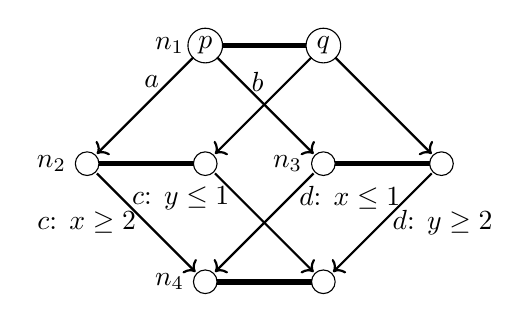
\begin{tikzpicture}[scale=1, every node/.style={transform shape}]

\begin{scope}[line width=2pt]
\draw (0,0) node [left] {$n_1\,\,$} -- (1.5,0);
\draw (-1.5,-1.5) node [left] {$n_2\,\,$} -- (0,-1.5);
\draw (1.5,-1.5) node [left] {$n_3\,\,$} -- (3,-1.5);
\draw (0,-3) node [left] {$n_4\,\,$} -- (1.5,-3);
\end{scope}

\filldraw [fill=white]  (0,0)  circle (2.2mm) node (n1p) {$p$};
\filldraw [fill=white]  (1.5,0)  circle (2.2mm) node (n1q) {$q$};

\filldraw [fill=white]  (-1.5,-1.5)  circle (1.5mm) node (n2p) {};
\filldraw [fill=white]  (0,-1.5)  circle (1.5mm) node (n2q) {};

\filldraw [fill=white]  (1.5,-1.5)  circle (1.5mm) node (n3p) {};
\filldraw [fill=white]  (3,-1.5)  circle (1.5mm) node (n3q) {};

\filldraw [fill=white]  (0,-3)  circle (1.5mm) node (n4p) {};
\filldraw [fill=white]  (1.5,-3)  circle (1.5mm) node (n4q) {};

\begin{scope}[thick,->]
\draw (n1p) + (-0.15,-0.15) -- (n2p) node [near start, left] {$a$};
\draw (n1q) + (-0.15,-0.15) -- (n2q);

\draw (n1p) + (0.15,-0.15) -- (n3p) node [near start, right] {$b$};
\draw (n1q) + (0.15,-0.15) -- (n3q);

\draw (n2p) -- (n4p) node [midway, left] {$c$: $x \geq 2$};
\draw (n2q) -- (n4q) node [near start, left] {$c$: $y \leq 1$};

\draw (n3p) -- (n4p) node [near start, right] {$d$: $x \leq 1$};
\draw (n3q) -- (n4q) node [midway, right] {$d$: $y \geq 2$};
\end{scope}

\end{tikzpicture}
\caption{Synchronization-free LTN illustrating implicit coordination. At $n_1$, agents $p$ and $q$ non-deterministically choose outcome $a$ or $b$. For outcome $c$ at $n_4$ to be feasible, both must have chosen $a$ (route through $n_2$), since $c$ requires $x \geq 2$ from $p$ and $y \leq 1$ from $q$—constraints incompatible with the $b$-route guards.}
\label{fig:coord}
\end{figure}

At $n_1$, outcome $a$ or $b$ is chosen non-deterministically. To reach location $(n_4, c)$, both agents must route through $n_2$ (both choosing $a$), since $c$ requires $x \geq 2$ from $p$ and $y \leq 1$ from $q$. Routing through $n_3$ (via outcome $b$) imposes $x \leq 1$ for $p$ and $y \geq 2$ for $q$. These constraints make $(n_4, c)$ unreachable if either agent chose $b$. Thus, local timing decisions at $n_1$ have global reachability consequences, even without explicit synchronization. The agents must implicitly `agree' on a path to make later locations feasible.

\subsection{Product-region abstraction}
\paragraph{Geometric intuition.}
In synchronization-free LTNs, each agent evolves according to its own
local clocks without ever comparing time with other agents.
Consequently, the global time state of the system can be seen as a tuple
of independent local time states—one per agent.

For each agent $p$, the standard region abstraction partitions
$\mathbb{R}_{\ge 0}^{X_p}$ into finitely many regions.
The global abstraction is then obtained by taking the Cartesian product
of these per-agent partitions.
Two global valuations are equivalent if and only if they are equivalent
for each agent separately.

Intuitively, synchronization-free LTNs behave like a collection of
independent timed automata whose discrete transitions must occur
together at negotiation nodes, but whose timing evolution is otherwise
decoupled.

Let
\[
  M := \max\{\,c \mid \text{$c$ appears in some atomic constraint $x\bowtie c$ of a guard in $\Nn$}\,\}.
\]
In this fragment, reference clocks $T=\{t_p\mid p\in P\}$ do not appear in guards
and are never tested for synchronization. Thus, for reachability, it suffices to
abstract only the local clocks $X$.

We define a region equivalence \emph{per agent} and take their product.

\begin{definition}[Per-agent region equivalence]
\label{def:per-agent-region}
Fix an agent $p \in P$. For valuations $v, v' : X_p \to \mathbb{R}_{\geq 0}$, write $v \sim^p_M v'$ if for all clocks $x, y \in X_p$:
\begin{enumerate}
\item \textbf{Integer parts agree (or both exceed $M$):} \\
Either $\lfloor v(x) \rfloor = \lfloor v'(x) \rfloor$, or both $\lfloor v(x) \rfloor > M$ and $\lfloor v'(x) \rfloor > M$.

\item \textbf{Zero fractional parts agree:} \\
If $v(x) \leq M$, then $\text{frac}(v(x)) = 0$ iff $\text{frac}(v'(x)) = 0$.

\item \textbf{Fractional orderings agree (for clocks $\leq M$):} \\
If $v(x) \leq M$ and $v(y) \leq M$, then $\text{frac}(v(x)) \leq \text{frac}(v(y))$ iff $\text{frac}(v'(x)) \leq \text{frac}(v'(y))$.
\end{enumerate}
\end{definition}

This is precisely the standard timed-automata region equivalence~\cite{DBLP:journals/tcs/AlurD94} applied to clocks $X_p$ of agent $p$.

\begin{definition}[Product-region equivalence]
\label{def:product-region}
For valuations $v, v' : X \to \mathbb{R}_{\geq 0}$ (over all local clocks), write $v \sim_{\text{pr}} v'$ if:
\[
v|_{X_p} \sim^p_M v'|_{X_p} \quad \text{for every agent } p \in P.
\]
We call $\sim_{\text{pr}}$ the \emph{product-region equivalence}. Let $[v]_{\text{pr}}$ denote the equivalence class of $v$.
\end{definition}

\begin{lemma}[Finite index]
\label{lem:size-of-product-regions}
The product-region equivalence $\sim_{\mathrm{pr}}$ has finite index. In
particular, the number of product-regions is bounded by
$\Oo(|X|!\cdot 2^{|X|}\cdot (2M+2)^{|X|})$.
\end{lemma}

%========================
% Lemma 5.3 (Finite index)
%========================
\begin{proof}[Proof of Lemma~\ref{lem:size-of-product-regions}]
Fix an agent $p\in P$ and let $k_p := |X_p|$.  We first bound the number of
$\sim^p_M$-classes over valuations of $X_p$, and then take the product over all
agents.

A $\sim^p_M$-class is determined by the following finite data:

\medskip\noindent
\textbf{(A) Truncated integer parts.}
For each $x\in X_p$, define its \emph{truncated integer part}
\[
  \iota(x) \;:=\;
  \begin{cases}
    \lfloor v(x)\rfloor & \text{if } \lfloor v(x)\rfloor \le M,\\
    M+1 & \text{if } \lfloor v(x)\rfloor > M.
  \end{cases}
\]
Thus $\iota(x)\in\{0,1,\dots,M,M+1\}$, giving at most $(M+2)^{k_p}$ possibilities.

\medskip\noindent
\textbf{(B) Zero/nonzero fractional flags for clocks not above $M$.}
For each $x\in X_p$ with $\iota(x)\le M$ we record the Boolean
\[
  z(x) \;:=\; \bigl( \{v(x)\}=0 \bigr).
\]
For clocks with $\iota(x)=M+1$ (i.e.\ $v(x)>M$) this flag is irrelevant in the
definition of $\sim^p_M$, so we may still count it pessimistically. This yields
at most $2^{k_p}$ possibilities.

\medskip\noindent
\textbf{(C) Ordering of fractional parts among clocks not above $M$.}
Let $S := \{x\in X_p \mid \iota(x)\le M\}$.
The third bullet in Definition~\ref{def:product-region} requires that for all
$x,y\in S$,
\[
  \{v(x)\}\le \{v(y)\} \quad\text{iff}\quad \{v'(x)\}\le \{v'(y)\}.
\]
Equivalently, it fixes the total preorder of the multiset
$\bigl(\{v(x)\}\bigr)_{x\in S}$.
Any total preorder on $|S|\le k_p$ elements can be obtained by taking a total
order and allowing ties; hence the number of such preorders is bounded by
$k_p!\cdot 2^{k_p}$ (choose an order, then choose where to merge adjacent items).
Therefore, the number of possibilities for (C) is at most $k_p!\cdot 2^{k_p}$.

\medskip
Combining (A), (B), (C), the number of $\sim^p_M$-classes is bounded by
\[
  (M+2)^{k_p}\cdot 2^{k_p}\cdot (k_p!\cdot 2^{k_p})
  \;=\; k_p!\cdot 2^{2k_p}\cdot (M+2)^{k_p}.
\]

Now $\sim_{\mathrm{pr}}$ is the product of the per-agent relations, so the number
of product-regions is at most the product over agents:
\[
  \prod_{p\in P} \Bigl(k_p!\cdot 2^{2k_p}\cdot (M+2)^{k_p}\Bigr)
  \;=\;
  \Bigl(\prod_{p} k_p!\Bigr)\cdot 2^{2\sum_p k_p}\cdot (M+2)^{\sum_p k_p}.
\]
Since $\sum_p k_p = |X|$ and $\prod_p k_p! \le |X|!$, we obtain
\[
  \#\text{(product-regions)} \;\le\; |X|!\cdot 2^{2|X|}\cdot (M+2)^{|X|}.
\]
Finally, using $M+2 \le 2M+2$ for $M\ge 0$ and absorbing the extra $2^{|X|}$ into
the $\mathcal{O}$-notation, we get the stated bound
\[
  \#\text{(product-regions)} \;=\; \mathcal{O}\bigl(|X|!\cdot 2^{|X|}\cdot (2M+2)^{|X|}\bigr).
\]
Hence $\sim_{\mathrm{pr}}$ has finite index.
\end{proof}

\begin{lemma}[Compatibility with local delays]
\label{lemma:region-local-delay}
Let $v \sim_{\mathrm{pr}} v'$. For every local delay vector $\Delta\in \Rpos^{P}$
there exists a local delay vector $\Delta'$ such that
$v+\Delta \sim_{\mathrm{pr}} v'+\Delta'$.
\end{lemma}

%\begin{proof}[Proof sketch]
%The claim follows componentwise from the standard time-elapse property of region equivalence for timed automata (Chapter~\ref{chap:preliminaries}): for each agent $p$, from $v|_{X_p}\sim^p_M v'|_{X_p}$ and the delay $\Delta(p)$ we obtain some $\Delta'(p)$ such that $v|_{X_p}+\Delta(p) \sim^p_M v'|_{X_p}+\Delta'(p)$. Taking the product over all agents yields the stated $\Delta'$.
%\end{proof}

%=========================================
% Lemma 5.4 (Compatibility with local delays)
%=========================================
\begin{proof}
Assume $v \sim_{\mathrm{pr}} v'$ and fix a local delay vector
$\Delta\in\Rpos^{P}$.
We construct a local delay vector $\Delta'\in\Rpos^{P}$ such that
$v+\Delta \sim_{\mathrm{pr}} v'+\Delta'$.

Fix an agent $p\in P$ and write $v_p := v|_{X_p}$ and $v'_p := v'|_{X_p}$.
By definition of $\sim_{\mathrm{pr}}$, we have $v_p \sim^p_M v'_p$.

Now consider the standard timed-automata region equivalence on the clock set
$X_p$ with maximal constant $M$; our relation $\sim^p_M$ is exactly this
equivalence (restricted to clocks of agent $p$).
By the time-elapse compatibility of regions proved in the preliminaries
(Lemma~\ref{lem:TA-region-time-elapse}), from $v_p \sim^p_M v'_p$ and
$d:=\Delta(p)\ge 0$ we obtain a delay $d'\ge 0$ such that
\[
  v_p + d \;\sim^p_M\; v'_p + d'.
\]
Define $\Delta'(p):=d'$.

Doing this independently for every agent $p$ yields a vector
$\Delta'\in \Rpos^{P}$ satisfying, for each $p$,
\[
  (v+\Delta)|_{X_p} \;=\; v_p+\Delta(p) \;\sim^p_M\; v'_p+\Delta'(p)
  \;=\; (v'+\Delta')|_{X_p}.
\]
Since $\sim_{\mathrm{pr}}$ is defined componentwise over agents, this implies
$v+\Delta \sim_{\mathrm{pr}} v'+\Delta'$, as required.
\end{proof}

\begin{lemma}[Compatibility with guards and resets]
\label{lem:region-guard-reset}
Let $v \sim_{\mathrm{pr}} v'$. Let $g$ be any guard whose constants are at most
$M$. Then:
\begin{enumerate}
  \item $v\models g$ iff $v'\models g$;
  \item for every set of local clocks $Y\subseteq X$, we have $v[Y]\sim_{\mathrm{pr}} v'[Y]$.
\end{enumerate}
\end{lemma}

%=========================================
% Lemma 5.5 (Compatibility with guards and resets)
%=========================================
\begin{proof}
Assume $v \sim_{\mathrm{pr}} v'$, and let $g$ be any guard whose constants are at
most $M$. By the syntax used in the chapter, $g$ is a Boolean combination of
atomic constraints of the form $x \bowtie c$ where $c\in\{0,1,\dots,M\}$ and
$\bowtie\in\{<,\le,=,\ge,>\}$, and $x$ is a local clock.

\medskip\noindent
\textbf{(1) Preservation of guard satisfaction.}
Since $g$ is a Boolean combination, it suffices to prove preservation for a
single atomic constraint $x\bowtie c$.

Fix such an atom. Let $p$ be the unique agent with $x\in X_p$.
From $v \sim_{\mathrm{pr}} v'$ we get $v|_{X_p} \sim^p_M v'|_{X_p}$, hence in
particular:
\begin{itemize}
  \item either $\lfloor v(x)\rfloor=\lfloor v'(x)\rfloor$, or both
        $\lfloor v(x)\rfloor > M$ and $\lfloor v'(x)\rfloor > M$;
  \item if $v(x)\le M$ then $\{v(x)\}=0$ iff $\{v'(x)\}=0$.
\end{itemize}

Now consider cases.

\smallskip\noindent
\emph{Case I: $v(x)>M$.}
Then $v'(x)>M$ as well. Since $c\le M$, we have $v(x)\bowtie c$ iff $v'(x)\bowtie c$
for all $\bowtie\in\{>,\ge\}$ (both true) and for all $\bowtie\in\{<,\le,=\}$
(both false). So the atom is preserved.

\smallskip\noindent
\emph{Case II: $v(x)\le M$.}
Then $\lfloor v(x)\rfloor=\lfloor v'(x)\rfloor=:k\le M$.
Write $v(x)=k+f$ and $v'(x)=k+f'$ with $f,f'\in[0,1)$ and $f=0$ iff $f'=0$.

Because $c$ is an integer, the truth of $x\bowtie c$ depends only on:
(i) whether $k<c$, $k>c$, or $k=c$; and (ii) in the boundary case $k=c$, whether
the fractional part is $0$ or not.

Indeed:
\begin{itemize}
  \item $v(x) < c$ iff $k<c$;
  \item $v(x) \le c$ iff $k<c$ or ($k=c$ and $f=0$);
  \item $v(x) = c$ iff $k=c$ and $f=0$;
  \item $v(x) \ge c$ iff $k>c$ or ($k=c$ and $f=0$);
  \item $v(x) > c$ iff $k>c$.
\end{itemize}
All these conditions are preserved when replacing $(k,f)$ by $(k,f')$ because
$k$ is the same and $f=0 \Leftrightarrow f'=0$.
Hence $v\models (x\bowtie c)$ iff $v'\models (x\bowtie c)$.

This proves preservation for atoms, hence for any Boolean combination $g$.

\medskip\noindent
\textbf{(2) Preservation under resets.}
Let $Y\subseteq X$ be any set of local clocks to reset to $0$.
We must show $v[Y]\sim_{\mathrm{pr}} v'[Y]$.

Fix an agent $p$. We show $(v[Y])|_{X_p} \sim^p_M (v'[Y])|_{X_p}$.
Let $Y_p := Y\cap X_p$. Then $(v[Y])|_{X_p}$ is obtained from $v|_{X_p}$ by
setting clocks in $Y_p$ to $0$ (and leaving others unchanged), and similarly for
$v'$.

Take any $x\in X_p$.
\begin{itemize}
  \item If $x\in Y_p$, then both valuations assign $0$ to $x$, so the first two
        bullets of $\sim^p_M$ hold trivially for $x$.
  \item If $x\notin Y_p$, then $v[Y](x)=v(x)$ and $v'[Y](x)=v'(x)$, so the first
        two bullets hold because they held for $v$ and $v'$.
\end{itemize}
For the third bullet (ordering of fractional parts among clocks $\le M$), note
that every reset clock has fractional part $0$, and every non-reset clock keeps
its old fractional part. Since in $v$ and $v'$ the relative order relations
$\{v(x)\}\le \{v(y)\}$ among clocks $\le M$ were identical, and since we apply
the same transformation “set some designated clocks to $0$” on both sides, the
resulting order relations among fractional parts remain identical as well.
Formally, for any $x,y\in X_p$ with $(v[Y])(x)\le M$ and $(v[Y])(y)\le M$:
\begin{itemize}
  \item if both are not reset, the relation is the same as before;
  \item if one is reset, its fractional part becomes $0$ on both sides;
  \item if both are reset, both fractional parts are $0$ on both sides.
\end{itemize}
Hence the iff-condition in the third bullet is preserved.

Therefore $(v[Y])|_{X_p}\sim^p_M (v'[Y])|_{X_p}$ for every $p$, i.e.\
$v[Y]\sim_{\mathrm{pr}} v'[Y]$.
\end{proof}

\subsection{The product-region automaton}

We now build a finite automaton over locations that captures precisely the
feasible untimed location sequences of a synchronization-free LTN.

\begin{definition}[Product-region automaton]
\label{def:pr-automaton}
Let $\mathcal{N}$ be synchronization-free. The \textsf{product-region automaton} $\mathcal{A}_{\text{pr}}(\mathcal{N})$ is an NFA with:
\begin{itemize}
\item \textbf{States}: pairs $(C, r)$ where $C$ is a marking and $r$ is a product-region.

\item \textbf{Transitions}: $(C, r) \xrightarrow{(n,a)} (C', r')$ iff there exist $v \in r$ and local delay $\Delta$ such that:
\[
(C, v) \xrightarrow{\Delta} (C, v + \Delta) \xrightarrow{(n,a)} (C', v')
\]
in $\mathcal{N}$, with $v' \in r'$.

\item \textbf{Initial state}: $(C_0, [v_0]_{\text{pr}})$ where $C_0(p) = \{n_{\text{in}}\}$ for all $p$, and $v_0$ maps all clocks in $X$ to 0.
\end{itemize}
\end{definition}

% ------------------------------------------------------------------
% Explicit product-region calculations for the running (sync-free) example
% (adapted to satisfy the "guards are local" assumption in this chapter)
% ------------------------------------------------------------------

\subsection{Product-Region Calculations on an Example}
\label{subsec:explicit-pr-example}

We illustrate the product-region abstraction (Section~\ref{sec:syncfree}) by
working out regions explicitly on a tiny synchronization-free LTN instance.
Recall that in our model, each agent's guard mentions only its own local clocks
(see Lemma~\ref{lem:product-region-compat}(2)).\,\footnote{This locality
assumption is used throughout this chapter.}

\paragraph{The example.}
Let $P=\{p,q\}$, with local clocks $X_p=\{x\}$ and $X_q=\{y\}$.
Consider three nodes $N=\{n_0,n_1,n_2\}$ with
\[
\dom(n_0)=\{p,q\},\qquad \dom(n_1)=\{p\},\qquad \dom(n_2)=\{p,q\}.
\]
We fix outcomes $a,b,c$ and local transition data:
\begin{itemize}
\item At $(n_0,a)$: no guards, no resets (only control-flow updates).
\item At $(n_1,b)$ (agent $p$ only): guard $x \ge 1$, reset $x:=0$.
\item At $(n_2,c)$ (agents $p,q$): for $q$ we require guard $y \ge 1$ and reset $y:=0$
      (agent $p$ has trivial guard/reset at this step).
\end{itemize}
This example is synchronization-free, i.e.\ $\Sync=\emptyset$.

\begin{figure}[htb]
\centering 
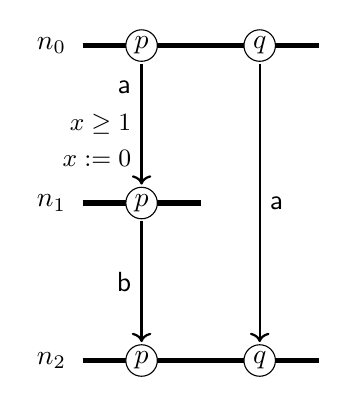
\begin{tikzpicture}[scale=1, every node/.style={transform shape}]

    % Nodes (Bars)
    \draw[line width=2pt] (0,4) node[left] {$n_0\,$} -- (3,4);
    \draw[line width=2pt] (0,2) node[left] {$n_1\,$} -- (1.5,2);
    \draw[line width=2pt] (0,0) node[left] {$n_2\,$} -- (3,0);

    % Ports
    \filldraw[fill=white] (0.75,4) circle (2mm) node (p_n0) {$p$};
    \filldraw[fill=white] (2.25,4) circle (2mm) node (q_n0) {$q$};
    
    \filldraw[fill=white] (0.75,2) circle (2mm) node (p_n1) {$p$};
    
    \filldraw[fill=white] (0.75,0) circle (2mm) node (p_n2) {$p$};
    \filldraw[fill=white] (2.25,0) circle (2mm) node (q_n2) {$q$};

    % Edges
    % p: n0 -> n1
    \draw[->, thick] (p_n0) -- (p_n1) node[midway, left, align=right] {$\mathsf{a}$ \\ \small $x \ge 1$ \\ \small $x:=0$};
    
    % q: n0 -> n2 (Wait)
    \draw[->, thick] (q_n0) -- (q_n2) node[midway, right] {$\mathsf{a}$};

    % p: n1 -> n2
    \draw[->, thick] (p_n1) -- (p_n2) node[midway, left] {$\mathsf{b}$};

\end{tikzpicture}
\caption{A simple synchronization-free LTN.}
\label{fig:coord}
\end{figure}

\paragraph{Maximal constant.}
The only constants appearing in guards are $1$, hence
\[
M = 1.
\]

\subsubsection*{Per-agent regions for one clock (with $M=1$)}
Since each agent has a single clock, the standard region
equivalence partitions $\mathbb{R}_{\ge 0}$ into four regions:
\begin{align*}
R^0 &:= \{z \mid z = 0\},\\
R^{(0,1)} &:= \{z \mid 0 < z < 1\},\\
R^{1} &:= \{z \mid z = 1\},\\
R^{>1} &:= \{z \mid z > 1\}.
\end{align*}
For agent $p$ (clock $x$) we write these as $R_x^0, R_x^{(0,1)}, R_x^{1}, R_x^{>1}$,
and similarly for agent $q$ (clock $y$) we write $R_y^0, R_y^{(0,1)}, R_y^{1}, R_y^{>1}$.

\subsubsection*{Product regions}
A product-region is a pair of per-agent regions:
\[
r \;=\; R_x^{\alpha}\times R_y^{\beta}
\qquad\text{where}\qquad
\alpha,\beta \in \{0,(0,1),1,>1\}.
\]
Hence there are $4\cdot 4 = 16$ product-regions in total.

\paragraph{Guard satisfaction at the region level.}
With $M=1$ and one clock per agent:
\[
x \ge 1 \text{ holds exactly on } R_x^1 \cup R_x^{>1},
\qquad
y \ge 1 \text{ holds exactly on } R_y^1 \cup R_y^{>1}.
\]
This is the concrete instantiation of Lemma~\ref{lem:product-region-compat}(2).

\subsubsection*{A concrete run and its product-region trace}
We now pick explicit local delays (a delay vector $\Delta\in\mathbb{R}_{\ge 0}^P$)
and track the induced product-region sequence.

\paragraph{Initial valuation.}
Let $v_0(x)=0$ and $v_0(y)=0$. Then
\[
(x,y)=(0,0)\in R_x^0\times R_y^0,
\quad\text{so}\quad
r_0 := [v_0]_{pr} = R_x^0\times R_y^0.
\]

\paragraph{Step 1: delay then $(n_1,b)$.}
Choose a local delay $\Delta_0$ with
\[
\Delta_0(p)=1.3,\qquad \Delta_0(q)=0.4.
\]
After delay, we have
\[
(x,y)=(1.3,0.4)\in R_x^{>1}\times R_y^{(0,1)},
\quad\text{so}\quad
r_1 = R_x^{>1}\times R_y^{(0,1)}.
\]
Now $(n_1,b)$ is enabled because $x\ge 1$ holds in $R_x^{>1}$.
Executing $(n_1,b)$ resets $x:=0$, yielding
\[
(x,y)=(0,0.4)\in R_x^0\times R_y^{(0,1)},
\quad\text{so}\quad
r_2 = R_x^0\times R_y^{(0,1)}.
\]

\paragraph{Step 2: delay then $(n_2,c)$.}
Choose a local delay $\Delta_1$ with
\[
\Delta_1(p)=0.2,\qquad \Delta_1(q)=0.8.
\]
After delay, we have
\[
(x,y)=(0.2,1.2)\in R_x^{(0,1)}\times R_y^{>1},
\quad\text{so}\quad
r_3 = R_x^{(0,1)}\times R_y^{>1}.
\]
Now $(n_2,c)$ is enabled because $y\ge 1$ holds in $R_y^{>1}$.
Executing $(n_2,c)$ resets $y:=0$, yielding
\[
(x,y)=(0.2,0)\in R_x^{(0,1)}\times R_y^0,
\quad\text{so}\quad
r_4 = R_x^{(0,1)}\times R_y^{0}.
\]

\paragraph{Region-trace summary.}
Altogether, this concrete run induces the product-region trace
\[
R_x^0\times R_y^0
\;\xrightarrow{\Delta_0=(1.3,\,0.4)}\;
R_x^{>1}\times R_y^{(0,1)}
\;\xrightarrow{(n_1,b):\,x\ge 1,\ x:=0}\;
R_x^{0}\times R_y^{(0,1)}
\;\xrightarrow{\Delta_1=(0.2,\,0.8)}\;
R_x^{(0,1)}\times R_y^{>1}
\;\xrightarrow{(n_2,c):\,y\ge 1,\ y:=0}\;
R_x^{(0,1)}\times R_y^{0}.
\]
This makes the product abstraction fully explicit: the global abstract state
changes by (i) componentwise time-elapse within each per-agent region partition,
followed by (ii) componentwise resets triggered by discrete steps.

\begin{lemma}[Soundness and completeness]
\label{lem:reg-prod-reg-equiv}
Assume $\Nn$ is synchronization-free.
\begin{enumerate}
  \item For every run of $\Nn$
  \[
  (C_0,v_0)\xra{\Delta_0,(n_0,a_0)}(C_1,v_1)\xra{\Delta_1,(n_1,a_1)}\cdots\xra{\Delta_{m-1},(n_{m-1},a_{m-1})}(C_m,v_m),
  \]
  there exists a run in $\prg(\Nn)$
  \[
  (C_0,\region{v_0})\xra{(n_0,a_0)}(C_1,\region{v_1})\xra{(n_1,a_1)}\cdots\xra{(n_{m-1},a_{m-1})}(C_m,\region{v_m}).
  \]
  \item Conversely, for every run in $\prg(\Nn)$
  \[
  (C_0,r_0)\xra{(n_0,a_0)}(C_1,r_1)\xra{(n_1,a_1)}\cdots\xra{(n_{m-1},a_{m-1})}(C_m,r_m),
  \]
  there exists a run in $\Nn$
  \[
  (C_0,v_0)\xra{\Delta_0,(n_0,a_0)}(C_1,v_1)\xra{\Delta_1,(n_1,a_1)}\cdots\xra{\Delta_{m-1},(n_{m-1},a_{m-1})}(C_m,v_m)
  \]
  such that $v_i\in r_i$ for all $0\le i\le m$.
\end{enumerate}
\end{lemma}

%=========================================
% Lemma 5.7 (Soundness and completeness)
%=========================================
\begin{proof}[Detailed proof of Lemma~\ref{lem:reg-prod-reg-equiv}]
Assume $\Nn$ is synchronization-free, so only local clocks $X$ matter and there
is no synchronization test involving reference clocks.

\medskip\noindent
\textbf{(1) Soundness (from $\Nn$ to $\prg(\Nn)$).}
Let
\[
(C_0,v_0)\xra{\Delta_0,(n_0,a_0)}(C_1,v_1)\xra{\Delta_1,(n_1,a_1)}\cdots
\xra{\Delta_{m-1},(n_{m-1},a_{m-1})}(C_m,v_m)
\]
be a run of $\Nn$.
By the LTN semantics, each macro-step
$\xra{\Delta_i,(n_i,a_i)}$ abbreviates a small-step decomposition
\[
(C_i,v_i)\xra{\Delta_i}(C_i,v_i+\Delta_i)\xra{(n_i,a_i)}(C_{i+1},v_{i+1}).
\]
Set $r_i:=\region{v_i}$ for each $i$.
By Definition~\ref{def:prod-reg-aut} of $\prg(\Nn)$, a transition
\[
(C_i,r_i)\xra{(n_i,a_i)}(C_{i+1},r_{i+1})
\]
exists whenever there are witnesses $v\in r_i$, $\Delta\ge 0$ such that
$(C_i,v)\xra{\Delta}(C_i,v+\Delta)\xra{(n_i,a_i)}(C_{i+1},v')$ with $v'\in r_{i+1}$.
We can take the concrete witnesses $v:=v_i$, $\Delta:=\Delta_i$, and $v':=v_{i+1}$.
Thus every step of the $\Nn$-run induces a corresponding step in $\prg(\Nn)$,
yielding the run
\[
(C_0,\region{v_0})\xra{(n_0,a_0)}(C_1,\region{v_1})\xra{(n_1,a_1)}\cdots
\xra{(n_{m-1},a_{m-1})}(C_m,\region{v_m}).
\]

\medskip\noindent
\textbf{(2) Completeness (from $\prg(\Nn)$ to $\Nn$).}
Let
\[
(C_0,r_0)\xra{(n_0,a_0)}(C_1,r_1)\xra{(n_1,a_1)}\cdots
\xra{(n_{m-1},a_{m-1})}(C_m,r_m)
\]
be a run of $\prg(\Nn)$.
We construct, by induction on $i=0,\dots,m$, valuations $v_i\in r_i$ and local
delays $\Delta_i$ (for $i<m$) such that
\[
(C_i,v_i)\xra{\Delta_i}(C_i,v_i+\Delta_i)\xra{(n_i,a_i)}(C_{i+1},v_{i+1})
\]
is a valid small-step decomposition in $\Nn$.

\smallskip\noindent
\emph{Base $i=0$.}
By construction of $\prg(\Nn)$, $r_0=\region{v_0}$ where $v_0$ is the all-zero
valuation, so choose $v_0$ accordingly.

\smallskip\noindent
\emph{Induction step.}
Assume $v_i\in r_i$ has been chosen.
Consider the automaton transition
\[
(C_i,r_i)\xra{(n_i,a_i)}(C_{i+1},r_{i+1}).
\]
By Definition~\ref{def:prod-reg-aut}, there exist witnesses:
a valuation $u_i\in r_i$, a local delay vector $\widehat{\Delta}_i$, and a
valuation $u_{i+1}\in r_{i+1}$ such that in $\Nn$,
\[
(C_i,u_i)\xra{\widehat{\Delta}_i}(C_i,u_i+\widehat{\Delta}_i)\xra{(n_i,a_i)}(C_{i+1},u_{i+1})
\]
is a valid pair of steps.

Now $v_i\in r_i$ and $u_i\in r_i$ imply $v_i \sim_{\mathrm{pr}} u_i$.
Apply Lemma~\ref{lemma:region-local-delay} to $v_i \sim_{\mathrm{pr}} u_i$ and
delay $\widehat{\Delta}_i$ to obtain a (possibly different) local delay vector
$\Delta_i$ such that
\[
v_i+\Delta_i \;\sim_{\mathrm{pr}}\; u_i+\widehat{\Delta}_i. \tag{$\ast$}
\]
We claim that $(n_i,a_i)$ is enabled from $(C_i, v_i+\Delta_i)$ and that firing it
produces some $v_{i+1}\in r_{i+1}$.

Let $g$ be the conjunction of all local guards required for executing outcome
$(n_i,a_i)$ (one per participating agent, combined as in the LTN semantics).
Since $\Nn$ is synchronization-free, $g$ depends only on local clocks and uses
only constants $\le M$ (by definition of $M$ in the chapter).
Because $u_i+\widehat{\Delta}_i$ enables $(n_i,a_i)$, we have
$u_i+\widehat{\Delta}_i \models g$.
By ($\ast$) and Lemma~\ref{lem:region-guard-reset}(1), we also have
$v_i+\Delta_i \models g$, hence $(n_i,a_i)$ is enabled from $(C_i,v_i+\Delta_i)$.

Let $Y\subseteq X$ be the set of local clocks reset by firing $(n_i,a_i)$
(across all agents in $\dom(n_i)$, exactly as prescribed by $\delta$).
In a synchronization-free LTN, the discrete step sets precisely those clocks in
$Y$ to $0$ and leaves the others unchanged; thus the successor valuation is
\[
v_{i+1} := (v_i+\Delta_i)[Y], \qquad
u_{i+1} := (u_i+\widehat{\Delta}_i)[Y].
\]
By Lemma~\ref{lem:region-guard-reset}(2) applied to ($\ast$), we get
\[
(v_i+\Delta_i)[Y] \;\sim_{\mathrm{pr}}\; (u_i+\widehat{\Delta}_i)[Y],
\]
i.e.\ $v_{i+1} \sim_{\mathrm{pr}} u_{i+1}$.
Since $u_{i+1}\in r_{i+1}$ and $r_{i+1}$ is a $\sim_{\mathrm{pr}}$-class, it
follows that $v_{i+1}\in r_{i+1}$, completing the induction step.

\smallskip
Thus we obtain a concrete $\Nn$-run
\[
(C_0,v_0)\xra{\Delta_0,(n_0,a_0)}(C_1,v_1)\xra{\Delta_1,(n_1,a_1)}\cdots
\xra{\Delta_{m-1},(n_{m-1},a_{m-1})}(C_m,v_m)
\]
with $v_i\in r_i$ for all $i$, proving completeness.
\end{proof}

\begin{theorem}
\label{thm:pspace-syncfree}
Location-reachability is \PSPACE-complete for synchronization-free LTNs.
\end{theorem}

\begin{proof}
Let $K$ denote the input size of $\Nn$, measured as the total encoding size of
nodes, outcomes, clocks, and the binary encodings of constants in guards.

\paragraph{Upper bound.}
By Lemma~\ref{lem:reg-prod-reg-equiv}, a location $\ell=(n,a)$ is reachable in
$\Nn$ iff it is reachable in the finite graph underlying $\prg(\Nn)$.
The number of markings is at most $2^{\Oo(|P|\cdot |N|)}$, hence
$2^{\Oo(K)}$, and the number of product-regions is $2^{\Oo(K)}$ by
Lemma~\ref{lem:size-of-product-regions}. Therefore $\prg(\Nn)$ has at most
$2^{\Oo(K)}$ states.

%Reachability in an exponentially large graph given by an on-the-fly successor procedure can be decided in polynomial space by a standard Savitch-style argument~\cite{SAVITCH1970177}. Hence location-reachability is in \PSPACE.

Although $\prg(\Nn)$ is exponentially large, each state has a polynomial-size
encoding and successors can be generated on the fly in polynomial space. Hence
we can decide reachability by a nondeterministic polynomial-space procedure:
start at the initial state, and for at most $2^m$ steps (where $m$ is the
encoding length) nondeterministically guess a successor and verify it using the
on-the-fly successor test; accept if a target state is reached. This uses only
polynomial space (current state plus an $m$-bit step counter), so the problem is
in $\NPSPACE$, and therefore in $\PSPACE$ by Savitch's theorem~\cite{SAVITCH1970177}.

\paragraph{Lower bound.}
\PSPACE-hardness follows from reachability in timed automata~\cite{DBLP:journals/tcs/AlurD94}.
A timed automaton can be encoded as an LTN with a single agent; with one agent,
local time coincides with global time and $\Sync=\emptyset$ vacuously. \qed
\end{proof}

%-------------------------------------------------------------------------------
\section{Always-synchronizing LTNs}
\label{sec:always-synchr-negot}

\subsection{Definition and Intuitive Behavior}

\begin{definition}[Always-synchronizing LTN]
An LTN $\Nn$ is \emph{always-synchronizing} if $\Sync = N$.
\end{definition}

In this fragment, when location $(n, a)$ is executed, all agents $p \in \text{dom}(n)$ must have equal reference clocks: $t_p = t_q$ for all $p, q \in \text{dom}(n)$. This essentially enforces a global timestamp for each interaction.

In the synchronization-free case, reference clocks were irrelevant. Here, they're central—but not in the way that caused undecidability. In general LTNs, synchronization is \emph{selective}. Some nodes synchronize, others don't. This allows building gadgets where agents drift apart (at unsynchronized nodes), then compare drifts (at synchronized nodes), simulating counter tests.
In always-synchronizing LTNs, synchronization is \emph{global}. Since every node synchronizes, reference clocks stay aligned throughout. There's no opportunity to accumulate unbounded drift between synchronized interactions. This is essentially a return to global-time semantics.

\paragraph{Need for different technique.} We cannot directly use the product-region construction from Section~\ref{sec:syncfree}, because:
\begin{enumerate}
\item Reference clocks now appear in constraints (synchronization $v(t_p) = v(t_q)$),
\item Standard region abstractions for TA rely on clock values beyond $M$ being safely abstractable until reset, but reference clocks are never reset.
\end{enumerate}

\paragraph{Key insight: monotone witnesses.} Timestamps are not monotone here. Despite of that, we can always reorder any run into one where interactions occur in increasing timestamp order. This ``monotone-by-time" property enables a reduction to global-time timed automata.

\subsection{Monotone runs}

\begin{definition}[Timestamp of a location and monotonicity]
\label{def:timestamp}
Let $\mathcal{N}$ be always-synchronizing. Consider a run:
\[
\rho = (C_0, v_0) \xrightarrow{\Delta_0, (n_0, a_0)} (C_1, v_1) \xrightarrow{\Delta_1, (n_1, a_1)} \cdots \xrightarrow{\Delta_{m-1}, (n_{m-1}, a_{m-1})} (C_m, v_m).
\]
The \textsf{timestamp} of location $(n_i, a_i)$ in $\rho$ is:
\[
\theta^\rho_i := (v_i + \Delta_i)(t_p) \quad \text{for any } p \in \text{dom}(n_i).
\]
This is well-defined because $n_i \in \text{Sync}$ implies all agents in $\text{dom}(n_i)$ have equal reference clocks at execution.

Run $\rho$ is \textsf{monotone} if $\theta^\rho_0 \leq \theta^\rho_1 \leq \cdots \leq \theta^\rho_{m-1}$.
\end{definition}

\paragraph{Intuition.} Since every node synchronizes, each discrete step occurs at a moment when all participating agents agree on ``what time it is". The timestamp records this agreed-upon moment. A monotone run executes locations in chronological order.

\begin{example}[A non-monotone run in the running example, and its monotone rearrangement]
\label{ex:nonmonotone-running}

We illustrate how non-monotone runs arise in always-synchronizing LTNs, using the
running two-agent example introduced earlier.

Recall that the running example has agents $p,q$, a $p$-only node $n_1$, and a
joint node $n_2$ with $\dom(n_2)=\{p,q\}$. For symmetry, we additionally consider
a $q$-only node $n_1'$ with $\dom(n_1')=\{q\}$ (this does not affect any reachability
results, and merely exposes the symmetry between the agents).

Assume that all guards are trivial and that no local clocks are reset at $n_1$,
$n_1'$, or $n_2$; we focus only on the behavior of reference clocks.

\smallskip
\noindent
\textbf{A non-monotone run.}
Consider the following execution fragment:
\begin{itemize}
  \item \emph{Step 1 (private step of $p$).}
  Agent $p$ delays for $8$ time units, while $q$ does not delay, and executes
  $(n_1,a_1)$.  
  Since the system is always-synchronizing, the timestamp of this step is
  \[
  \theta_1 = t_p = 8.
  \]

  \item \emph{Step 2 (private step of $q$).}
  Next, agent $q$ delays for $7$ time units, while $p$ does not delay, and executes
  $(n_1',a_1')$.  
  The timestamp of this step is
  \[
  \theta_2 = t_q = 7.
  \]
\end{itemize}
Thus $\theta_1 > \theta_2$, and the run is non-monotone. Note that this does not
contradict monotonicity of any single agent's reference clock: the inversion
occurs between two actions whose domains are disjoint, since
\[
\dom(n_1)\cap\dom(n_1')=\emptyset.
\]

\smallskip
\noindent
\textbf{Reordering into a monotone run.}
Because $(n_1,a_1)$ and $(n_1',a_1')$ involve disjoint agents, their delays, guards,
resets, and marking updates are independent and commute. We may therefore swap the
two steps to obtain the following execution:
\begin{itemize}
  \item First execute $(n_1',a_1')$ at timestamp $\theta_2=7$.
  \item Then execute $(n_1,a_1)$ at timestamp $\theta_1=8$.
\end{itemize}
This reordered run is monotone, since $7 \le 8$.

\smallskip
\noindent
\textbf{Effect on subsequent synchronization.}
After either ordering of the two private steps, the reference-clock valuation is
the same:
\[
t_p=8,\qquad t_q=7.
\]
Consequently, any subsequent execution of the joint node $(n_2,a_2)$ behaves
identically in both runs: the agent with the smaller reference clock is forced to
wait until the clocks synchronize before $(n_2,a_2)$ can occur.

This example concretely illustrates the key phenomenon used in the proof of
Theorem~\ref{thm:monotone-witness}: inversions can arise only between actions with
disjoint domains, and such inversions can always be eliminated by swapping
independent steps.

Here $\theta_1 = 8 > \theta_2 = 7$, so the run is non-monotone. But since $\text{dom}(n_1) \cap \text{dom}(n_2) = \{p\} \neq \emptyset$... wait, actually this can't happen! If $p$ participates in both, then $t_p$ must increase, so $\theta_2 \geq \theta_1$. The key observation (proven below) is that inversions only occur between actions involving disjoint agents.
\end{example}

\begin{lemma}[Inversions involve disjoint domains]
\label{lem:inversion-disjoint}
Let $\rho$ be a run of an always-synchronizing LTN. If $\theta^\rho_i > \theta^\rho_{i+1}$ for some $i$, then $\text{dom}(n_i) \cap \text{dom}(n_{i+1}) = \emptyset$.
\end{lemma}

\begin{proof}
Suppose $p \in \text{dom}(n_i) \cap \text{dom}(n_{i+1})$. Reference clocks never reset and only increase via local delays. After step $i$, agent $p$ has reference clock $(v_i + \Delta_i)(t_p) = \theta^\rho_i$. Before step $i+1$, $p$ undergoes delay $\Delta_{i+1}(p) \geq 0$, reaching reference clock $(v_{i+1} + \Delta_{i+1})(t_p) = \theta^\rho_i + \Delta_{i+1}(p) \geq \theta^\rho_i$. But $(v_{i+1} + \Delta_{i+1})(t_p) = \theta^\rho_{i+1}$ (by definition of timestamp for step $i+1$), so $\theta^\rho_{i+1} \geq \theta^\rho_i$, contradicting $\theta^\rho_i > \theta^\rho_{i+1}$. \qed
\end{proof}

\paragraph{Timeline intuition.}
In always-synchronizing LTNs, every interaction occurs at a moment when
all participating agents agree on the current reference time.
Thus, each executed location can be assigned a global timestamp.

Although different agents may perform independent actions at different
times, any apparent reordering of timestamps can only arise between
actions involving disjoint sets of agents.
Such actions are causally independent: their guards, resets, and marking
updates affect disjoint components of the system.

As a result, any run can be rearranged—by repeatedly swapping adjacent
independent steps—into a run where timestamps are non-decreasing.
This monotone form reveals an underlying global-time structure,
enabling a reduction to timed automata.

\begin{lemma}[Existence of monotone witnesses]
\label{lem:monotonic}
For every location $(n,a)$ that is reachable in an always-synchronizing LTN
$\Nn$, there exists a \emph{monotone} run of $\Nn$ that executes $(n,a)$.
\end{lemma}

%-------------------------------------------------------------------------------
% Lemma 5.11 / Lemma \ref{lem:monotonic}: Existence of monotone witnesses
%-------------------------------------------------------------------------------
\begin{proof}[Proof of Lemma~\ref{lem:monotonic}]
Fix any run $\rho$ of $\Nn$ that executes the target location $(n,a)$.
Write the discrete steps of $\rho$ as
\[
(C_0,v_0)\xra{\Delta_0}(C_0,w_0)\xra{\ell_0}(C_1,v_1)\xra{\Delta_1}(C_1,w_1)\xra{\ell_1}\cdots
\xra{\Delta_{m-1}}(C_{m-1},w_{m-1})\xra{\ell_{m-1}}(C_m,v_m),
\]
where $w_i := v_i+\Delta_i$ and $\ell_i=(n_i,a_i)$.
For each $i$, let $D_i := \dom(n_i)$ and let $\theta_i := \theta^\rho_i$ be the
timestamp of $\ell_i$ (Definition~\ref{def:monotone-run}), i.e.\
$\theta_i = w_i(t_p)$ for any $p\in D_i$.

\medskip\noindent
\textbf{Step 1: A normal form for delays (``tight'' runs).}
We first transform $\rho$ into a run $\widehat\rho$ with the \emph{same} sequence
$\ell_0,\ldots,\ell_{m-1}$ of discrete steps, such that for every $i$,
\[
\widehat\Delta_i(p)=0 \quad\text{whenever } p\notin D_i,
\]
i.e.\ the delay before $\ell_i$ is applied only by agents that actually
participate in $\ell_i$.

This is done by repeatedly pushing \emph{irrelevant} delay components to the
right: suppose for some $i$ and some agent $p\notin D_i$ we have
$\Delta_i(p)=\delta>0$. Since $p$ does not participate in $\ell_i$, the enabling
of $\ell_i$ and all its guards/resets are independent of the clocks of $p$.
Moreover, reference clocks are never reset, and local clocks of $p$ are neither
tested nor reset by $\ell_i$ (as $p\notin D_i$). Hence we can replace the pair
of consecutive delay vectors $(\Delta_i,\Delta_{i+1})$ by
\[
\Delta_i' := \Delta_i - \delta\cdot \mathbf{e}_p,
\qquad
\Delta_{i+1}' := \Delta_{i+1} + \delta\cdot \mathbf{e}_p,
\]
(where $\mathbf{e}_p$ is the unit vector for agent $p$), and obtain another
valid run with the same discrete step sequence. Intuitively, we simply postpone
a portion of $p$'s waiting time across an action that does not involve $p$.
This preserves all clock values for all agents at every discrete step in which
they participate, hence preserves satisfaction of all guards and yields the same
marking evolution.

Iterating this operation finitely many times (pushing each irrelevant component
to the next delay until it reaches a step where that agent participates, or the
end) yields a run $\widehat\rho$ in the desired normal form. Importantly,
timestamps of steps are unchanged by this normalization because $\theta_i$
depends only on agents in $D_i$ and we never move delay components of agents in
$D_i$ away from the position immediately preceding $\ell_i$.

From now on, replace $\rho$ by this normalized run and keep the same notation.

\medskip\noindent
\textbf{Step 2: Inversions can only happen between disjoint domains.}
We claim that if $\theta_i>\theta_{i+1}$, then $D_i\cap D_{i+1}=\emptyset$.
Indeed, if $p\in D_i\cap D_{i+1}$, then $p$ participates in both steps.
Reference clocks are never reset and only increase by nonnegative local delays.
Therefore $w_{i+1}(t_p)\ge w_i(t_p)$. But $w_i(t_p)=\theta_i$ and
$w_{i+1}(t_p)=\theta_{i+1}$ by definition of timestamp, contradicting
$\theta_i>\theta_{i+1}$.

\medskip\noindent
\textbf{Step 3: Swapping an adjacent inversion.}
Assume there is an index $i$ with $\theta_i>\theta_{i+1}$. By Step~2,
$D_i\cap D_{i+1}=\emptyset$. Since we are in the normal form,
$\Delta_i$ has support included in $D_i$ and $\Delta_{i+1}$ has support included
in $D_{i+1}$. Consider the local fragment
\[
(C_i,v_i)\xra{\Delta_i}(C_i,w_i)\xra{\ell_i}(C_{i+1},v_{i+1})
\xra{\Delta_{i+1}}(C_{i+1},w_{i+1})\xra{\ell_{i+1}}(C_{i+2},v_{i+2}).
\]
Because $D_i$ and $D_{i+1}$ are disjoint:
\begin{itemize}
\item executing $\ell_i$ does not read/reset/update clocks of agents in $D_{i+1}$,
      and executing $\ell_{i+1}$ does not read/reset/update clocks of agents in $D_i$;
\item the marking update of $\ell_i$ changes only the components $C(p)$ for
      $p\in D_i$, and the marking update of $\ell_{i+1}$ changes only the
      components $C(p)$ for $p\in D_{i+1}$, hence the two marking updates commute;
\item the delay vector $\Delta_i$ affects only agents in $D_i$, and $\Delta_{i+1}$
      affects only agents in $D_{i+1}$, hence the two delays commute and each can
      be moved across the other's discrete action without affecting its guards.
\end{itemize}
Therefore we can swap the two \emph{blocks} $(\Delta_i,\ell_i)$ and
$(\Delta_{i+1},\ell_{i+1})$ to obtain another valid run fragment
\[
(C_i,v_i)\xra{\Delta_{i+1}}(C_i,\widetilde w_{i+1})\xra{\ell_{i+1}}(C_{i+1}',\widetilde v_{i+1})
\xra{\Delta_{i}}(C_{i+1}',\widetilde w_{i})\xra{\ell_i}(C_{i+2},v_{i+2}),
\]
that reaches the \emph{same} configuration $(C_{i+2},v_{i+2})$ as before.
Moreover, the timestamp of $\ell_{i+1}$ in the swapped fragment remains
$\theta_{i+1}$ (since the participants in $D_{i+1}$ experience exactly the same
total delay before executing $\ell_{i+1}$), and similarly the timestamp of
$\ell_i$ remains $\theta_i$. Hence the adjacent inversion at positions $i,i+1$
is eliminated.

\medskip\noindent
\textbf{Step 4: Bubble-sort to obtain monotonicity.}
Define the number of \emph{adjacent inversions} of the timestamp sequence
$\theta_0,\ldots,\theta_{m-1}$ as
\[
Inv(\rho) := \bigl|\{\,i \mid 0\le i<m-1,\ \theta_i>\theta_{i+1}\,\}\bigr|.
\]
If $Inv(\rho)=0$, the run is monotone and we are done.
Otherwise, Step~3 produces a new run with the same set of discrete steps (in
particular still executing $(n,a)$) and strictly smaller $Inv(\cdot)$, because
we remove at least the chosen adjacent inversion and do not create any new
inversion involving steps whose domains overlap (Step~2 prevents that).
Since $Inv(\rho)$ is a natural number, iterating this operation finitely many
times yields a run with $Inv=0$, i.e.\ a monotone run that executes $(n,a)$.

This proves the lemma.
\end{proof}

\paragraph{Why this helps.} Monotone runs have a global-time interpretation: locations occur in chronological order. This allows us to simulate the entire LTN with a single timed automaton using global time.

\subsection{Reduction to timed automata}

We now construct a timed automaton that recognizes exactly the monotone runs of
$\Nn$ (projected to locations). Intuitively, the always-synchronizing constraint
forces all participating agents to act at the same timestamp, which corresponds
to the global-time view of a single timed automaton.

\begin{definition}[Timed automaton of an always-synchronizing LTN]
\label{def:ta-always}
Let $\Nn$ be always-synchronizing. Define a timed automaton $\ta(\Nn)$ as follows:
\begin{itemize}
  \item States are all markings of $\Nn$; write $Q$ for this set.
  \item The alphabet is the set of locations: $\Sigma_{\ta} := N\times \Sigma$.
  \item The clock set is the same local-clock set $X$ (reference clocks are not needed).
  \item The initial state is the initial marking $C_0$.
  \item Transitions are defined as follows. There is a transition
  \[
     (C,\, (n,a),\, g,\, Y,\, C')
  \]
  iff:
  \begin{enumerate}
    \item $n$ is enabled in $C$, i.e.\ $n\in C(p)$ for all $p\in\dom(n)$;
    \item for each $p\in \dom(n)$, $\delta_p(n,a)=(g_p,M_p,Y_p)$, and
          $g := \bigwedge_{p\in\dom(n)} g_p$ and $Y := \bigcup_{p\in\dom(n)} Y_p$;
    \item $C'(p)=M_p$ for $p\in\dom(n)$ and $C'(p)=C(p)$ for $p\notin\dom(n)$.
  \end{enumerate}
\end{itemize}
\end{definition}

\paragraph{Intuition.} The TA simulates the LTN in "global time." Each LTN node becomes a TA transition. Since nodes synchronize, all participating agents act at the same global timestamp—which is exactly what TA semantics provides. Local clocks $X_p$ advance with global time, just as they advanced with (synchronized) reference times in the LTN.

\begin{lemma}[Correctness of the reduction]
\label{lem:ta-for-always-sync}
Let $\Nn$ be always-synchronizing. A location $(n,a)$ is reachable in $\Nn$ iff
$\ta(\Nn)$ has a run that executes a transition labeled by $(n,a)$.
\end{lemma}


%-------------------------------------------------------------------------------
% Lemma 5.13 / Lemma \ref{lem:ta-for-always-sync}: Correctness of the reduction
%-------------------------------------------------------------------------------
\begin{proof}[Proof of Lemma~\ref{lem:ta-for-always-sync}]
We show both directions.

\medskip\noindent
\textbf{(\texorpdfstring{$\Rightarrow$}{=>}) If $(n,a)$ is reachable in $\Nn$, then $\ta(\Nn)$ executes $(n,a)$.}
Assume $(n,a)$ is reachable in $\Nn$. By Lemma~\ref{lem:monotonic}, there exists
a \emph{monotone} run $\rho$ of $\Nn$ that executes $(n,a)$.
Write $\rho$ as in Definition~\ref{def:monotone-run}, with discrete steps
$\ell_i=(n_i,a_i)$ and timestamps
\[
\theta_0 \le \theta_1 \le \cdots \le \theta_{m-1}.
\]
Let $\theta_{-1}:=0$ and define global delays
\[
d_i := \theta_i-\theta_{i-1} \quad \text{for } i=0,\ldots,m-1.
\]
Monotonicity ensures $d_i\ge 0$.

We now construct a run of $\ta(\Nn)$ that takes the same sequence of labels
$\ell_0,\ldots,\ell_{m-1}$ with those global delays.
Let $u_0$ be the all-zero valuation of the TA clocks $X$.
Inductively, suppose we are at TA state $C_i$ with valuation $u_i$. We let time
elapse by $d_i$, reaching valuation $u_i+d_i$.
We claim that the transition of $\ta(\Nn)$ labeled $\ell_i=(n_i,a_i)$ is enabled
at $(C_i,u_i+d_i)$, and taking it yields $(C_{i+1},u_{i+1})$.

To see this, first note that $C_i$ in the TA is the same marking as in the LTN
run, hence $n_i$ is enabled in $C_i$ (Definition~\ref{def:ta-always}(2.1)).
Next, let the local rule for each $p\in D_i:=\dom(n_i)$ be
$\delta_p(n_i,a_i)=(g_p,M_p,Y_p)$, and let $g=\bigwedge_{p\in D_i} g_p$ and
$Y=\bigcup_{p\in D_i} Y_p$ as in Definition~\ref{def:ta-always}(2.2).

The key observation is that in a monotone run, the value of any local clock
$x\in X_p$ at the execution of $\ell_i$ depends only on the timestamp $\theta_i$
and the most recent timestamp at which $x$ was reset (by an earlier discrete
step involving $p$). Indeed, local clocks advance exactly with agent $p$'s local
time (reference time) and are reset only when $p$ participates; in particular,
between the last reset time $\theta_j$ of $x$ and $\theta_i$, the elapsed local
time of $p$ is exactly $\theta_i-\theta_j$, so $x$ has value $\theta_i-\theta_j$.

In the timed automaton run we are constructing, clocks in $X$ advance with the
global time, and the reset set on label $\ell_j$ is exactly the union of the
LTN resets at that step. Therefore, by induction on $i$, for every agent $p$ and
every clock $x\in X_p$, the value of $x$ in the TA valuation just before taking
$\ell_i$ is \emph{exactly the same} as the value of $x$ in the LTN run at
timestamp $\theta_i$ (both equal $\theta_i-\theta_j$ where $\theta_j$ is the last
reset timestamp of $x$).

Since each guard $g_p$ uses only clocks in $X_p$, it follows that
the LTN satisfaction $w_i\models g_p$ (which holds because $\rho$ executes
$\ell_i$) implies $(u_i+d_i)\models g_p$. Hence $(u_i+d_i)\models g$ and the TA
transition labeled $\ell_i$ is enabled. Taking it updates the marking to $C_{i+1}$
as in Definition~\ref{def:ta-always}(2.3) and resets exactly the clocks in $Y$,
matching the LTN reset effect. This defines $u_{i+1}$ and maintains the
induction invariant.

Thus $\ta(\Nn)$ has a run that executes $\ell_k=(n,a)$ for the appropriate index
$k$.

\medskip\noindent
\textbf{(\texorpdfstring{$\Leftarrow$}{<=}) If $\ta(\Nn)$ executes $(n,a)$, then $(n,a)$ is reachable in $\Nn$.}
Assume $\ta(\Nn)$ has a run
\[
(C_0,u_0)\xra{d_0}(C_0,u_0+d_0)\xra{\ell_0}(C_1,u_1)\xra{d_1}\cdots
\xra{d_{m-1}}(C_{m-1},u_{m-1}+d_{m-1})\xra{\ell_{m-1}}(C_m,u_m),
\]
where some $\ell_k=(n,a)$ occurs.
We build a run of $\Nn$ that executes the same discrete steps in the same order,
using \emph{uniform} local delays. For each $i$, define the local delay vector
$\Delta_i\in\Rpos^P$ by $\Delta_i(p):=d_i$ for all agents $p\in P$.

Start from the LTN initial configuration $(C_0,v_0)$ where all local clocks in
$X$ are $0$ and all reference clocks $t_p$ are $0$.
At step $i$, apply the local delay $\Delta_i$. This advances every agent's
reference clock by the \emph{same} amount $d_i$, hence for every node (and in
particular for $n_i$) the synchronization constraint $t_p=t_q$ over
$p,q\in\dom(n_i)$ is satisfied at the moment of execution.
Moreover, since local clocks in $X$ advance at the same rate as reference time
for each agent, after the delay $\Delta_i$ the valuation of all clocks in $X$
coincides with the TA valuation after global delay $d_i$.

Now consider the discrete step $\ell_i=(n_i,a_i)$. By construction of
$\ta(\Nn)$, the TA guard on $\ell_i$ is the conjunction of the participating
agents' guards. Since the TA transition is enabled, this conjunction holds; hence
each individual local guard $g_p$ holds for $p\in\dom(n_i)$ in the LTN valuation
as well. Therefore $\ell_i$ is enabled in $\Nn$ and can be executed, producing
exactly the same marking update as in the TA transition definition and resetting
exactly the same set of clocks in $X$.

Iterating this for all $i$ yields an LTN run that executes $\ell_k=(n,a)$.
Hence $(n,a)$ is reachable in $\Nn$.

\medskip
Combining both directions proves the lemma.
\end{proof}

\begin{theorem}
\label{thm:pspace-always}
Location-reachability is \PSPACE-complete for always-synchronizing LTNs.
\end{theorem}

\begin{proof}
By Lemma~\ref{lem:ta-for-always-sync}, it suffices to decide reachability of a
transition labeled $(n,a)$ in $\ta(\Nn)$.

Let $K$ be the input size of $\Nn$ (as in Theorem~\ref{thm:pspace-syncfree}).
The number of markings is at most $2^{\Oo(K)}$, hence $|Q|=2^{\Oo(K)}$.
The clock set is $X$, and maximal constants are bounded by those in $\Nn$.
Therefore the region graph of $\ta(\Nn)$ has at most
$|Q|\cdot 2^{\Oo(K)} = 2^{\Oo(K)}$ nodes. Reachability in this exponentially
large region graph can be checked in polynomial space via on-the-fly exploration,
yielding the \PSPACE\ upper bound.

\PSPACE-hardness again follows from timed automata reachability: a timed automaton
is an LTN with a single agent, and in that case $\Sync=N$ holds vacuously. \qed
\end{proof}

%-------------------------------------------------------------------------------
%\section{Conclusion}
%\label{sec:fragments-conclusion}

%We analyzed two extreme synchronization regimes for LTNs. In the synchronization-free fragment, reference clocks are irrelevant for reachability, and a product-region construction yields a finite abstraction.  In the always-synchronizing fragment, synchronization couples agents through reference times, but every reachable location admits a monotone witness run, allowing a reduction to timed automata reachability.  Both fragments are \PSPACE-complete. These results motivate the study of intermediate fragments that allow a controlled mix of synchronizing and non-synchronizing nodes while retaining decidability.

%-------------------------------------------------------------------------------

\section{Summary and perspective}
\label{sec:fragments-summary}

We have established PSPACE-completeness for both synchronization-free and always-synchronizing LTNs (Theorems~\ref{thm:pspace-syncfree} and ~\ref{thm:pspace-always}). Both match the complexity of timed automata, but via fundamentally different proof techniques. This section synthesizes the main lessons.

\subsection{Comparing the Two Fragments}

\begin{center}
\begin{tabular}{|l|p{5cm}|p{5cm}|}
\hline
\textbf{Property} & \textbf{Sync-Free} & \textbf{Always-Sync} \\
\hline
Synchronization & None ($\text{Sync} = \emptyset$) & Universal ($\text{Sync} = N$) \\
\hline
Reference clocks & Irrelevant (never tested) & Central (globally aligned) \\
\hline
Key structure & Clocks independent per agent & Global timeline emerges \\
\hline
Abstraction & Product of per-agent regions & Monotone witness runs \\
\hline
Technique & Componentwise quotient & Reduction to global time \\
\hline
Complexity & PSPACE-complete & PSPACE-complete \\
\hline
Expressiveness & Local constraints only & Enforces temporal alignment \\
\hline
\end{tabular}
\end{center}

\subsection{Why Both Are PSPACE (Not Lower, Not Higher)}

\paragraph{Why not lower than PSPACE?} Both fragments inherit the essential difficulty of timed automata: reasoning about continuous time with finite representations. The region/zone abstractions yield exponentially many equivalence classes, and reachability in exponentially large graphs is PSPACE-complete. The concurrency structure of negotiations (multiple agents, complex control flow) doesn't reduce this complexity—it just changes how we build the abstraction.

\paragraph{Why not higher than PSPACE (avoiding undecidability)?} 

\textbf{Sync-free case}: Reference clocks never interact. Each agent's timing is independent, preventing any mechanism to encode or compare unbounded values. The product abstraction succeeds because there's no cross-agent timing dependency.

\textbf{Always-sync case}: Reference clocks stay globally aligned. While agents can "wait" for each other, they can't accumulate unbounded relative drift that persists across interactions. Every interaction resets the playing field—all participating agents synchronize. The monotone-witness property shows this is equivalent to global time, where standard TA techniques apply.

\paragraph{What's missing for undecidability?} Both fragments avoid the dangerous combination:
\begin{itemize}
\item \textbf{Unbounded drift} + \textbf{selective synchronization}
\end{itemize}

In sync-free LTNs, there's no synchronization to test accumulated drift. In always-sync LTNs, there's no opportunity to accumulate unbounded drift between synchronized interactions. General LTNs allow both, enabling counter-machine simulations.

\subsection{The Design Space}

These extremes bracket a spectrum of possible restrictions:

\begin{center}
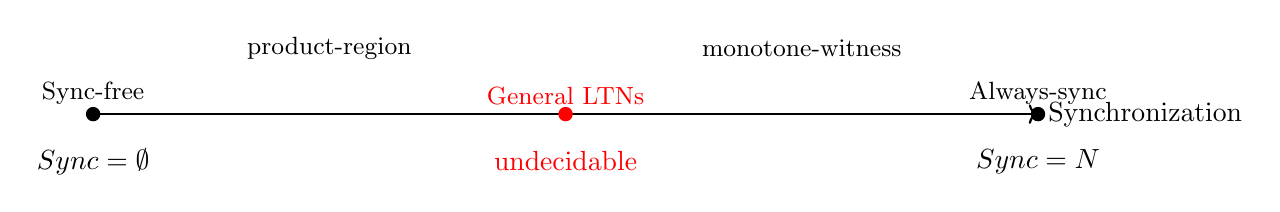
\begin{tikzpicture}[scale=1.2]
\draw[thick, ->] (0,0) -- (10,0) node[right] {Synchronization};
\node at (0,-0.5) {$\text{Sync} = \emptyset$};
\node at (10,-0.5) {$\text{Sync} = N$};
\filldraw (0,0) circle (2pt) node[above] {\small Sync-free};
\filldraw (10,0) circle (2pt) node[above] {\small Always-sync};
\filldraw[red] (5,0) circle (2pt) node[above] {\small General LTNs};
\node[red] at (5,-0.5) {undecidable};
\node at (2.5,0.7) {\small product-region};
\node at (7.5,0.7) {\small monotone-witness};
\end{tikzpicture}
\end{center}

\paragraph{Intermediate fragments.} What about LTNs where some nodes synchronize and others don't ($\emptyset \subset \text{Sync} \subset N$)? Two approaches:

\textbf{1. Quantitative restrictions (Chapter~\ref{chap:drift}):} Bound how much drift can accumulate, even with selective synchronization. If differences $t_p - t_q$ stay bounded, finite abstractions may still exist.

\textbf{2. Structural restrictions (Chapter~\ref{chap:connected}):} Require that control-flow structure prevents "problematic" patterns. For instance, demand that every cycle includes enough synchronization to prevent unbounded drift accumulation.

%-------------------------------------------------------------------------------

\section{Coming next}
\label{sec:fragments-coming-next}

This chapter established \PSPACE-completeness at the two extremes of
synchronization: when synchronization is absent, timing constraints remain
purely local and admit a product-region abstraction; when every node
synchronizes, every reachable location has a monotone witness run and
reachability reduces to timed-automata reachability.

\smallskip
In the next chapter we move to a genuinely intermediate regime: the
\emph{bounded-drift} fragment, where the deviation between agents' reference
times is globally bounded. We show how this quantitative restriction can be
exploited to recover a finite abstraction for reachability, and we analyze the
resulting complexity.



%\chapter{Drift-Bounded and Acyclic Local-Timed Negotiations}
\label{chap:drift-bounded}

\section{Introduction: From Synchronization to Drift}

The previous chapters established a sharp dichotomy in the decidability landscape of local-timed negotiations based on synchronization patterns:

\begin{itemize}
\item \textbf{Chapter~\ref{chap:ltn}}: General LTNs have undecidable reachability. The undecidability proof encodes counter values as \emph{differences between reference clocks}, exploiting unbounded drift combined with selective synchronization to test and manipulate these differences.

\item \textbf{Chapter~\ref{chap:fragments}}: Both synchronization extremes—synchronization-free ($\text{Sync} = \emptyset$) and always-synchronizing ($\text{Sync} = N$)—yield PSPACE-complete reachability. The synchronization-free fragment avoids drift accumulation by preventing clock comparisons across agents, while the always-synchronizing fragment enforces tight coupling that precludes the selective testing needed for counter simulation.
\end{itemize}

These results point to a natural question: rather than restricting synchronization patterns syntactically, can we instead control the \emph{semantic consequence} that makes undecidability possible—namely, unbounded divergence between reference clocks? If reference clocks can diverge arbitrarily, they can encode unbounded counters. But if their divergence remains bounded by some constant $k$ along all executions, then reference clock differences range over a finite domain $[-k, k]$, potentially enabling finite abstraction techniques analogous to region constructions for timed automata.

This chapter develops this intuition systematically, introducing \emph{drift-bounded LTNs} as a semantic restriction that cuts across synchronization patterns. The key insight is that boundedness of drift—the maximum difference between any two agents' reference clocks—can restore decidability even in the presence of partial synchronization, provided every discrete behavior admits at least one timed realization with bounded drift.

\subsection*{Chapter Overview and Contributions}

This chapter makes the following contributions:

\paragraph{Semantic restriction: $k$-drift boundedness.} We formalize drift as the maximum pairwise difference between reference clocks and introduce an \emph{existential} notion of $k$-drift boundedness (Definition~\ref{def:retiming-bounded}): an LTN is $k$-drift bounded if every discrete run admits at least one timed realization in which drift never exceeds $k$. This retiming-based notion, standard in the timed automata literature, focuses on time-abstract behaviors and enables reasoning about reachability via finite abstractions.

\paragraph{Finite abstraction and decidability.} For $k$-drift bounded LTNs, we adapt region-equivalence techniques to construct a finite $k$-region automaton that preserves reachability (Section~\ref{sec:k-regions}). This yields our first main result:

\begin{theorem}[Decidability for drift-bounded LTNs]
\label{thm:drift-main-result}
For each fixed $k \in \mathbb{N}$, location reachability for $k$-drift bounded LTNs is PSPACE-complete.
\end{theorem}

\paragraph{Structural implication: acyclic LTNs.} We then investigate when drift boundedness can be guaranteed structurally. We show that \emph{acyclicity}—the absence of cycles in the marking graph—implicitly enforces bounded drift (Corollary~\ref{cor:acyclic-drift-bounded}), even though acyclicity imposes no explicit constraints on timing or clock values. For acyclic LTNs, reachability becomes significantly simpler:

\begin{theorem}[Complexity for acyclic LTNs]
\label{thm:acyclic-np-complete}
Location reachability for acyclic local-timed negotiations is NP-complete.
\end{theorem}

The reduction from NP-completeness (for acyclic) to PSPACE-completeness (for general $k$-drift bounded) reflects the difference between systems where boundedness is structurally guaranteed versus those where it must be verified semantically.

\paragraph{Meta-complexity.} We also investigate the complexity of verifying drift boundedness itself, showing that checking whether an LTN satisfies a universal drift bound is PSPACE-complete, while determining the existence of such a bound is undecidable (Section~\ref{sec:drift-meta}).

\subsection*{Significance and Perspective}

Drift-bounded LTNs represent a shift from \emph{syntactic} restrictions (forbidding or mandating synchronization) to \emph{semantic} restrictions (bounding divergence in reachable behaviors). This perspective has several advantages:

\begin{itemize}
\item \textbf{Unification:} Drift boundedness subsumes and explains the decidability of both synchronization extremes studied in Chapter~\ref{chap:fragments}. Synchronization-free LTNs are trivially drift-bounded because independent clocks never need to converge; always-synchronizing LTNs enforce bounded drift through constant resynchronization.

\item \textbf{Generality:} Unlike synchronization-based restrictions, drift boundedness applies to systems with \emph{partial} synchronization—the most common case in practice, where some but not all interactions require coordination.

\item \textbf{Connection to structure:} The acyclicity result demonstrates that semantic properties (bounded drift) can arise from purely structural constraints (absence of control cycles), providing a bridge between syntax and semantics.
\end{itemize}

The remainder of this chapter is organized as follows. Section~\ref{sec:drift-def} formalizes drift and drift-bounded runs, with geometric intuition and concrete examples. Section~\ref{sec:k-drift-fragment} introduces the $k$-drift bounded fragment and establishes decidability via region abstraction. Section~\ref{sec:acyclic} studies acyclic LTNs as a structurally drift-bounded class and proves NP-completeness. Section~\ref{sec:drift-meta} investigates the decidability of drift boundedness verification. Section~\ref{sec:drift-summary} summarizes the chapter and previews the structural communication restrictions studied in Chapter~\ref{chap:connected-communication}.

\section{Drift: Definition, Intuition, and Examples}
\label{sec:drift-def}

In local-timed negotiations, each agent maintains a local reference clock that tracks its cumulative elapsed time. These clocks evolve independently during local delays and can therefore diverge. The extent of this divergence is captured by the notion of \emph{drift}.

\begin{definition}[Drift]
\label{def:drift}
Given a valuation $v$ over clocks including reference clocks $\{t_p\}_{p \in P}$, the \emph{drift} of $v$ is
\[
  \drift(v) := \max_{p,q \in P} |v(t_p) - v(t_q)|.
\]
A configuration $(C,v)$ is \emph{$k$-drift bounded}, for $k\in\Nat$, if $\drift(v) \le k$.
\end{definition}

Intuitively, drift measures how far apart agents' reference times can be at any given configuration. When drift is unbounded, the differences $v(t_p) - v(t_q)$ can encode arbitrary integers, enabling counter simulation and leading to undecidability (as demonstrated in Chapter~\ref{chap:ltn}).

\subsection{Geometric Intuition}

\begin{figure}[t]
    \centering
    
    % --- Subfigure 1: Unbounded Drift ---
    \begin{subfigure}[b]{0.45\textwidth}
        \centering
        \resizebox{\textwidth}{!}{%
        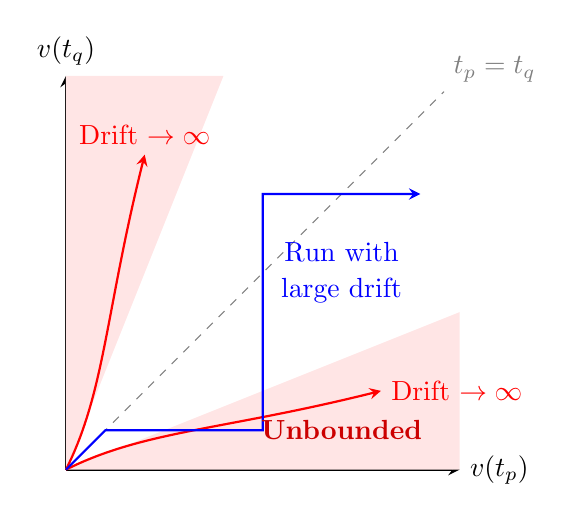
\begin{tikzpicture}[>=stealth]
            % Axes
            \draw[->, thick] (0,0) -- (5,0) node[right] {$v(t_p)$};
            \draw[->, thick] (0,0) -- (0,5) node[above] {$v(t_q)$};
            
            % Diagonal (Reference)
            \draw[dashed, gray] (0,0) -- (4.8,4.8) node[above right] {$t_p = t_q$};
            
            % Unbounded Region
            \fill[red!10] (0,0) -- (5,2) -- (5,0) -- cycle; 
            \fill[red!10] (0,0) -- (2,5) -- (0,5) -- cycle;
            
            \draw[red, thick, ->] (0,0) .. controls (1,0.5) and (2,0.5) .. (4,1) node[right] {Drift $\to \infty$};
            \draw[red, thick, ->] (0,0) .. controls (0.5,1) and (0.5,2) .. (1,4) node[above] {Drift $\to \infty$};
            
            % Sample Run
            \draw[thick, blue, ->] (0,0) -- (0.5, 0.5) -- (2.5, 0.5) -- (2.5, 3.5) -- (4.5, 3.5);
            \node[blue, align=center] at (3.5, 2.5) {Run with\\large drift};
            
            % Annotation
            \node[align=center, text=red!80!black] at (3.5, 0.5) {\textbf{Unbounded}};
        \end{tikzpicture}
        }
        \caption{\textbf{Unbounded Drift.} The difference $|v(t_p) - v(t_q)|$ can grow arbitrarily. Reachable states diverge far from the diagonal $t_p = t_q$, requiring infinite state space to track all possibilities.}
        \label{fig:drift_unbounded}
    \end{subfigure}
    \hfill
    % --- Subfigure 2: Bounded Drift ---
    \begin{subfigure}[b]{0.45\textwidth}
        \centering
        \resizebox{\textwidth}{!}{%
        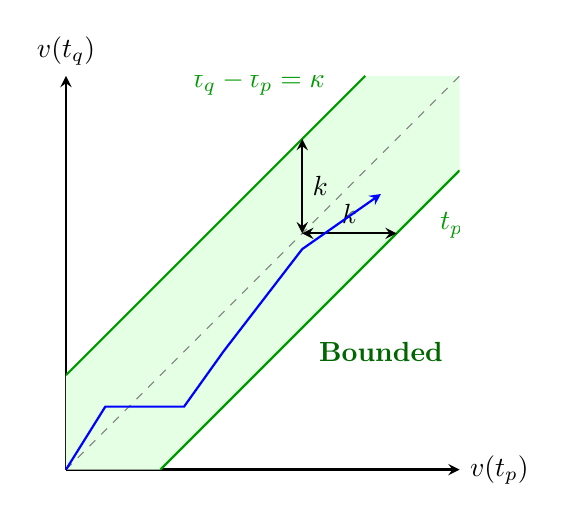
\begin{tikzpicture}[>=stealth]
            % Axes
            \draw[->, thick] (0,0) -- (5,0) node[right] {$v(t_p)$};
            \draw[->, thick] (0,0) -- (0,5) node[above] {$v(t_q)$};
            
            % Definitions
            \def\driftK{1.2}
            
            % The Band
            \begin{scope}
                \clip (0,0) rectangle (5,5);
                
                % Fill the valid band
                \fill[green!10] (0,0) -- (5,5) -- (5-\driftK, 5) -- (0, \driftK) -- cycle;
                \fill[green!10] (0,0) -- (5,5) -- (5, 5-\driftK) -- (\driftK, 0) -- cycle;
                
                % Draw the boundary lines
                \draw[thick, green!60!black] (0, \driftK) -- (5-\driftK, 5) node[pos=0.9, above left] {$t_q - t_p = k$};
                \draw[thick, green!60!black] (\driftK, 0) -- (5, 5-\driftK) node[pos=0.9, below right] {$t_p - t_q = k$};
            \end{scope}
            
            % Diagonal
            \draw[dashed, gray] (0,0) -- (5,5);
            
            % Arrows indicating bound
            \draw[<->, thick] (3,3) -- (3, 3+\driftK) node[midway, right] {$k$};
            \draw[<->, thick] (3,3) -- (3+\driftK, 3) node[midway, above] {$k$};

            % Sample Run
            \draw[thick, blue, ->] (0,0) -- (0.5, 0.8) -- (1.5, 0.8) -- (2.0, 1.5) -- (3.0, 2.8) -- (4.0, 3.5);
            
            % Annotation
            \node[align=center, text=green!40!black] at (4, 1.5) {\textbf{Bounded}};
        \end{tikzpicture}
        }
        \caption{\textbf{Bounded Drift ($k$-bounded).} All reachable configurations satisfy $|v(t_p) - v(t_q)| \le k$. States are confined to a diagonal band of width $2k$, enabling finite region abstraction.}
        \label{fig:drift_bounded}
    \end{subfigure}
    
    \caption{Geometric interpretation of drift in the space of reference clocks. The axes represent reference-clock values $v(t_p)$ and $v(t_q)$ for two agents. Although both values grow unboundedly over time, $k$-drift boundedness constrains their relative positions.}
    \label{fig:drift_comparison}
\end{figure}

Figure~\ref{fig:drift_comparison} visualizes drift in a two-agent system as a trajectory in the $(v(t_p), v(t_q))$ plane. The diagonal $v(t_p) = v(t_q)$ represents perfect synchronization.

\paragraph{Unbounded drift (left).} Without restrictions, executions may diverge arbitrarily far from the diagonal. The reachable region is potentially the entire quadrant, yielding an unbounded two-dimensional state space. This illustrates why standard region abstractions fail: tracking unbounded clock differences requires infinitely many regions, and these differences can encode counter values.

\paragraph{Bounded drift (right).} Under a drift bound $|v(t_p) - v(t_q)| \le k$, reachable configurations are constrained to an infinite strip of fixed width around the diagonal. Although time itself grows unboundedly, the \emph{relative positions} of reference clocks remain bounded. Crucially, this strip can be collapsed into a finite abstraction by quotienting time elapse, which is precisely what the $k$-region construction exploits (Section~\ref{sec:k-regions}).

\subsection{Motivating Examples}

To make drift boundedness concrete, we present two examples that illustrate the difference between unbounded and bounded drift at the level of simple control structures.

\begin{example}[Unbounded vs.\ bounded drift]
\label{ex:drift}
Figure~\ref{fig:abc} shows two LTNs over agents $p$ and $q$ that differ only in their timing constraints and synchronization patterns.

\paragraph{LTN $\Nn_1$ (left): Unbounded drift.} Nodes $n_1$ and $n_2$ both have self-loops labeled $a$ and $b$ respectively, each with guard $x = 1$ (or $y = 1$) and reset set $\{x\}$ (or $\{y\}$). For any $k \ge 0$, agent $p$ can execute the $a$-loop on $n_1$ exactly $k+1$ times while agent $q$ does not execute its $b$-loop at all. At the resulting configuration, node $n_3$ becomes enabled, but the reference-clock difference satisfies
\[
  |v(t_p)-v(t_q)| \;\ge\; k.
\]
Hence, the drift can grow arbitrarily large along reachable configurations.

Moreover, this drift cannot be reduced afterward. If agent $q$ allows more than one unit of local time to elapse while agent $p$ continues executing $a$-loops, then $q$ will violate the guard of its $b$-loop and can no longer perform it. Consequently, any run realizing the word $a^{k+1}b^{k+1}$ necessarily maintains drift at least $k$ throughout its execution, demonstrating that unbounded drift is intrinsic to the system's behavior.

\paragraph{LTN $\Nn_2$ (right): Bounded drift.} The structure is similar, but $\Nn_2$ enforces bounded drift through the time-synchronizing node $n_3$ (shown with a dotted line, indicating synchronization). Whenever $n_3$ is executed, the reference clocks of $p$ and $q$ are synchronized to the same value, so $\drift(v) = 0$ at that point. After synchronization, agent $p$ must wait at least 2 time units before executing $a$ (guard $x \ge 2$), while agent $q$ must execute $b$ within 1 time unit (guard $y \le 1$). This creates a maximum drift of $2 - 1 = 1$.

Repeating this synchronization pattern ensures that all reachable configurations of $\Nn_2$ satisfy $\drift(v) \le 1$, regardless of how many times the agents cycle through their behaviors.

    \begin{figure}[h]
        \centering
        \begin{minipage}{.45\textwidth}
        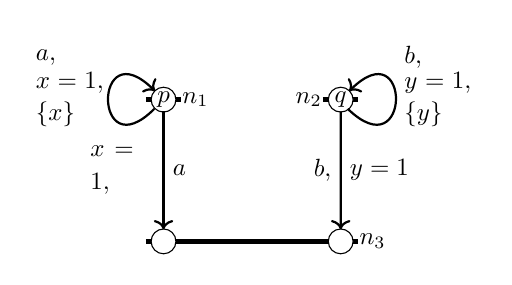
\begin{tikzpicture}[scale=0.9, every node/.style={transform shape}]
        
        \begin{scope}[line width=2pt]
        \draw (-.25,0) -- (0.25,0);
        \draw (2.25,0) -- (2.75,0);
        \draw (-.25,-2) -- (2.75,-2);
        \end{scope}
        
        \filldraw [fill=white]  (0,0)  circle (1.75mm) node (pa) {$p$};
        \filldraw [fill=white]  (2.5,0)  circle (1.75mm) node (qb) {$q$};
        \filldraw [fill=white]  (0,-2)  circle (1.75mm) node (pc) {};
        \filldraw [fill=white]  (2.5,-2)  circle (1.75mm) node (qc) {};
        
        \node at (0.45,0) {$n_1$};
        \node at (2.05,0) {$n_2$};
        \node at (2.95,-2) {$n_3$};
        \node at (-1.3,0.6) [text width=1cm] {$a,$};
        \node at (3.9,0.6) [text width=1cm] {$b,$};
        \node at (-1.3,0) [text width=1cm] {$x=1,$ $\{x\}$};
        \node at (3.9,0) [text width=1cm] {$y=1,$ $\{y\}$};
        
        \begin{scope}[thick,->]
        \draw (pa) + (0,-.165) -- (0,-1.83) node [midway, right] {$a$} node [midway, left, text width=0.9cm] {$x=1,$};
        \draw (qb) + (0,-.165) -- (2.5,-1.83) node [midway, left] {$b,$} node [midway, right, text width = 0.9cm] {$y=1$};
        \draw (-0.13,-0.13) .. controls (-1,-1) and (-1,1) .. (-0.12,0.12);
        \draw (2.6,-0.13) .. controls (3.5,-1) and (3.5,1) .. (2.62,0.12);
        \end{scope}
        
        \end{tikzpicture}
        \end{minipage}
        \begin{minipage}{.45\textwidth}
        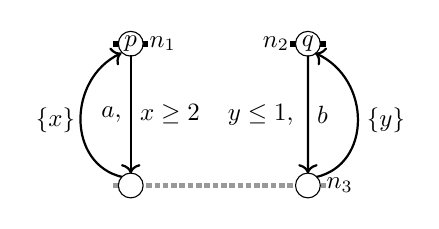
\begin{tikzpicture}[scale=0.9, every node/.style={transform shape}]
        
        \begin{scope}[line width=2pt]
        \draw (-.25,0) -- (0.25,0);
        \draw (2.25,0) -- (2.75,0);
        \draw [opacity=0.4, densely dotted] (-.25,-2) -- (2.75,-2);
        \end{scope}
        
        \filldraw [fill=white]  (0,0)  circle (1.75mm) node (pa) {$p$};
        \filldraw [fill=white]  (2.5,0)  circle (1.75mm) node (qb) {$q$};
        \filldraw [fill=white]  (0,-2)  circle (1.75mm) node (pc) {};
        \filldraw [fill=white]  (2.5,-2)  circle (1.75mm) node (qc) {};
        
        \node at (0.45,0) {$n_1$};
        \node at (2.05,0) {$n_2$};
        \node at (2.95,-2) {$n_3$};
        
        \begin{scope}[thick,->]
        \draw (pa) + (0,-.165) -- (0,-1.83) node [midway, left] {$a,$} node [midway, right, text width=0.85cm] {$x \ge 2$};
        \draw (qb) + (0,-.165) -- (2.5,-1.83) node [midway, right] {$b$} node [midway, left, text width = 1cm] {$y \le 1,$};
        \draw (pc) + (-0.12, 0.12) .. controls (-0.9,-1.7) and (-0.9,-0.5) .. (-0.13, -0.13) node [midway, left, text width=0.5cm] {$\{x\}$};
        \draw (qc) + (0.12, 0.12) .. controls (3.4,-1.7) and (3.4,-0.5) .. (2.6, -0.13) node [midway, right, text width=0.5cm] {$\{y\}$};
        \end{scope}
        
        \end{tikzpicture}
        \end{minipage}
        \caption{LTN $\Nn_1$ with unbounded drift (left) and $1$-drift bounded LTN $\Nn_2$ (right). The dotted line in $\Nn_2$ indicates a synchronizing interaction.}
            \label{fig:abc}
        \end{figure}
\end{example}

\begin{example}[ATM transaction with bounded drift]
\label{ex:atm-bounded-drift}
Consider the ATM transaction LTN from Figure~\ref{fig:ATM} (Chapter~\ref{chap:ltn}) with three agents: customer $c$, ATM $a$, and bank $b$. The negotiation exhibits partial synchronization—some interactions involve all three agents, while others involve only pairs.

\textbf{Claim:} This LTN is 10-drift bounded (assuming appropriate guard constants).

\textbf{Intuition:} 
\begin{itemize}
\item The customer $c$ can delay at most 10 units between interactions (guard $x \leq 10$ at outcome $\mathsf{e\_otp}$).
\item The bank $b$ can delay at most 3 units between interactions (guards $y \leq 3$ at $\mathsf{match}$ and $\mathsf{fail}$).
\item The ATM $a$ coordinates both, so its reference clock stays between $t_c$ and $t_b$.
\item Maximum drift occurs when $c$ is at $t_c = 10$ and $b$ hasn't started ($t_b = 0$), giving $\drift = 10$.
\item Subsequent interactions force resynchronization, preventing unbounded divergence.
\end{itemize}

This example illustrates that drift boundedness is compatible with partial synchronization and does not require the extreme restrictions of synchronization-free or always-synchronizing LTNs.
\end{example}

\subsection{Drift-Bounded Runs and LTNs}

We now formalize drift boundedness for runs and systems.

\begin{definition}[$k$-drift-bounded run]
\label{def:drift-bounded-run}
A run
\[
  \rho = (C_1,v_1)\xra{(\Delta_1,e_1)}(C_2,v_2)\xra{(\Delta_2,e_2)}\cdots
\]
is \emph{$k$-drift bounded} if every configuration $(C_i,v_i)$ occurring in the run satisfies $\drift(v_i) \le k$.
\end{definition}

The central notion studied in this chapter is an \emph{existential}, \emph{retiming-based} boundedness condition, standard in the timed-automata literature.

\begin{definition}[$k$-drift-bounded LTN]
\label{def:retiming-bounded}
An LTN $\Nn$ is \emph{$k$-drift bounded} if for every run
\[
  \rho = (C_1,v_1)\xra{\Delta_1,e_1}(C_2,v_2)\xra{\Delta_2,e_2}\cdots
\]
of $\Nn$, there exists a run
\[
  \rho_k = (C_1,v_1)\xra{\Delta'_1,e_1}(C_2,v'_2)\xra{\Delta'_2,e_2}\cdots
\]
with the same sequence of discrete outcomes $e_1, e_2, \ldots$, obtained by modifying only the local delays, such that $\rho_k$ is $k$-drift bounded.
\end{definition}

Thus, an LTN is $k$-drift bounded if every discrete behavior (untimed sequence of outcomes) admits at least one timed realization in which drift never exceeds~$k$.

\paragraph{Existential vs.\ universal drift boundedness.}
Definition~\ref{def:retiming-bounded} uses an \emph{existential} notion: we require that \emph{some} timed realization of each discrete behavior is drift-bounded, not that \emph{all} realizations are. This is the appropriate notion for reasoning about time-abstract behaviors via retiming and aligns with standard practice in timed automata verification.

In contrast, a \emph{universal} notion would require \emph{every reachable configuration} to satisfy the drift bound. Universal drift boundedness is stronger and less commonly satisfied, but it is also a natural property to verify (see Section~\ref{sec:drift-meta}). Throughout this chapter, "drift-bounded" without qualification means existentially drift-bounded.

\section{The $k$-Drift Bounded Fragment}
\label{sec:k-drift-fragment}

We now establish decidability and complexity for the class of $k$-drift bounded LTNs. The key insight is that bounded drift enables a finite abstraction analogous to region constructions for timed automata.

\subsection{Region Abstraction Under Bounded Drift}
\label{sec:k-regions}

Fix a constant $k\in\Nat$ and let $M$ be the maximum constant appearing in any clock constraint of $\Nn$. We adapt the region equivalence from networks of timed automata~\cite{DBLP:conf/concur/HerbreteauSW22} to LTNs.

\begin{definition}[$k$-Drift region equivalence $\cong_M^k$]
\label{def:k-region-equiv}
Let $M$ be the maximal constant in guards and $k$ the drift bound. Two $k$-drift bounded valuations $v, v'$ are equivalent, written $v \cong_M^k v'$, if:
\begin{enumerate}
    \item \textbf{Integral parts of local clocks:} For all $x \in \bigcup_{p \in P} X_p$, either $\lfloor v(x) \rfloor = \lfloor v'(x) \rfloor$ or both exceed $M$.
    
    \item \textbf{Fractional ordering:} For all clocks $x, y \in \bigcup_{p \in P} (X_p \cup \{t_p\})$, we have $\{v(x)\} \leq \{v(y)\}$ if and only if $\{v'(x)\} \leq \{v'(y)\}$, and equality of fractional parts is preserved: $\{v(x)\} = \{v(y)\}$ iff $\{v'(x)\} = \{v'(y)\}$.
    
    \item \textbf{Reference clock differences:} For all agents $p, q \in P$, we have $\lfloor v(t_p) - v(t_q) \rfloor = \lfloor v'(t_p) - v'(t_q) \rfloor$.
\end{enumerate}
\end{definition}

Although LTNs use explicit local clocks rather than the offset representation common in timed automata, the equivalence $\cong_M^k$ captures the same essential information:
\begin{itemize}
\item Condition (1) abstracts local clock values by their integer parts up to $M$, beyond which guards cease to distinguish values.
\item Condition (2) preserves the ordering of fractional parts, which determines the order in which clocks become integral and thus which guards become enabled.
\item Condition (3) tracks integer differences between reference clocks, which are bounded by $k$ under drift boundedness and determine synchronization constraints.
\end{itemize}

The key property of $\cong_M^k$ is that it is a \emph{time-abstract bisimulation} on the space of $k$-drift-bounded configurations: if $(C,v) \cong_M^k (C,v')$, then
\begin{enumerate}
\item For every local delay $\Delta$ from $(C,v)$, there exists a delay $\Delta'$ from $(C,v')$ such that $(C,v+\Delta) \cong_M^k (C,v'+\Delta')$.
\item $v$ satisfies a guard with constants at most $M$ if and only if $v'$ does.
\item For every synchronizing outcome, the equality constraints $v(t_p) = v(t_q)$ for participants $p, q$ are preserved under equivalent valuations.
\end{enumerate}

Consequently, for every $k$-drift-bounded run starting from $(C,v)$, there exists a $k$-drift-bounded run with the same discrete behavior starting from any $(C,v')$ with $(C,v) \cong_M^k (C,v')$.

\begin{lemma}[Finiteness of $\cong_M^k$]
\label{lem:finite-regions}
The equivalence $\cong_M^k$ has finitely many equivalence classes. Specifically, the number of regions is bounded by
\[
O\bigl( |N| \cdot 2^{|X|} \cdot |X|! \cdot (2M+1)^{|X|} \cdot (2k+1)^{|P|^2} \bigr),
\]
where $|N|$ is the number of nodes, $|X| = \sum_{p \in P} |X_p|$ is the total number of local clocks, and $|P|$ is the number of agents.
\end{lemma}

\begin{proof}
Each region is determined by:
\begin{itemize}
\item A marking $C$ (at most $|N|$ possibilities).
\item Integer parts of local clocks up to $M$ (at most $(M+2)^{|X|}$ possibilities, accounting for values $> M$).
\item An ordering of fractional parts among $|X| + |P|$ clocks (at most $(|X| + |P|)!$ orderings, and $2^{|X|+|P|}$ to record which are zero).
\item Integer differences $\lfloor t_p - t_q \rfloor$ for all pairs, bounded by $k$ (at most $(2k+1)^{|P|^2}$ combinations).
\end{itemize}
The product of these bounds yields an exponential dependence on $|X|$ and $|P|$, but polynomial in $M$ and $k$ when these are treated as parameters.
\end{proof}

\subsection{The $k$-Region Automaton}
\label{sec:k-automaton}

Using equivalence classes of $\cong_M^k$ as states, we construct a finite \emph{$k$-region automaton} $\mathcal{R}_k(\Nn)$ whose transitions abstract both time elapse and discrete outcomes.

\begin{definition}[$k$-Region automaton]
The $k$-region automaton $\mathcal{R}_k(\Nn)$ is a finite automaton with:
\begin{itemize}
\item \textbf{States:} Equivalence classes $[C,v]_{\cong_M^k}$ of $k$-drift bounded configurations.
\item \textbf{Initial state:} $[C_0, v_0]_{\cong_M^k}$ where $(C_0, v_0)$ is the initial configuration.
\item \textbf{Transitions:} $[C,v]_{\cong_M^k} \xrightarrow{e} [C',v']_{\cong_M^k}$ if there exist representatives $(C,v)$ and delays $\Delta, \Delta'$ such that $(C, v + \Delta) \xrightarrow{e} (C', v' + \Delta')$ and both configurations are $k$-drift bounded.
\end{itemize}
\end{definition}

The time-abstract bisimulation property ensures that reachability in $\mathcal{R}_k(\Nn)$ faithfully represents reachability of discrete behaviors in the original LTN.

\begin{theorem}[Soundness and completeness of $\mathcal{R}_k(\Nn)$]
\label{thm:region-automaton-correct}
A marking $C$ is reachable in $\Nn$ via a $k$-drift bounded run if and only if some region $[C,v]_{\cong_M^k}$ is reachable in $\mathcal{R}_k(\Nn)$.
\end{theorem}

\begin{proof}[Proof sketch]
\emph{Soundness:} If $[C,v]_{\cong_M^k}$ is reachable in $\mathcal{R}_k(\Nn)$, then by definition of transitions, there exists a corresponding $k$-drift bounded run in $\Nn$ reaching $(C,v)$.

\emph{Completeness:} If $C$ is reachable via a $k$-drift bounded run $\rho$ in $\Nn$, then by the bisimulation property, there exists an equivalent run through region representatives that witnesses reachability of $[C,v]_{\cong_M^k}$ in $\mathcal{R}_k(\Nn)$.
\end{proof}

\subsection{Decidability and Complexity}
\label{sec:drift-complexity}

We now establish the main complexity result for $k$-drift bounded LTNs.

\begin{theorem}[Main result for drift-bounded LTNs]
\label{thm:drift-pspace}
For each fixed $k \in \mathbb{N}$, location reachability is PSPACE-complete for $k$-drift bounded LTNs.
\end{theorem}

\begin{proof}
\textbf{PSPACE Upper Bound:} 
By Lemma~\ref{lem:finite-regions}, the $k$-region automaton has exponentially many states (in $|X|$ and $|P|$, polynomial in $M$ and $k$). Reachability in this finite automaton can be solved by a nondeterministic algorithm that guesses a path, storing only the current region at each step. This requires polynomial space: $O(\log(|N| \cdot |X|! \cdot M^{|X|} \cdot k^{|P|^2}))$, which is polynomial in the size of the LTN encoding. By Savitch's theorem, NPSPACE = PSPACE, yielding the upper bound.

\textbf{PSPACE Lower Bound:} 
A standard timed automaton $\mathcal{A}$ can be viewed as a single-agent LTN $\Nn_{\mathcal{A}}$. With only one agent, drift is trivially 0 (bounded). Location reachability for timed automata is PSPACE-complete~\cite{AlurDill94}, so reachability in $k$-drift bounded LTNs is PSPACE-hard.
\end{proof}

This result positions drift-bounded LTNs at the same complexity level as timed automata, despite their greater structural flexibility in modeling multi-agent interactions.

\section{Deciding Drift Boundedness}
\label{sec:drift-meta}

A natural meta-question is whether drift boundedness itself can be effectively verified. We consider four variants:

\begin{enumerate}
\item \textbf{Universal $k$-boundedness (fixed $k$):} Given $\Nn$ and $k$, is every reachable configuration $k$-drift bounded?
\item \textbf{Universal boundedness (existence of $k$):} Given $\Nn$, does there exist $k$ such that all reachable configurations are $k$-drift bounded?
\item \textbf{Existential $k$-boundedness (fixed $k$):} Given $\Nn$ and $k$, does every discrete behavior admit a $k$-drift bounded realization? (This is Definition~\ref{def:retiming-bounded}.)
\item \textbf{Existential boundedness (existence of $k$):} Given $\Nn$, does there exist $k$ such that $\Nn$ is existentially $k$-drift bounded?
\end{enumerate}

We address the first two questions here; the existential variants remain open but are less central to practical verification.

\subsection{Universal $k$-Drift Boundedness (Fixed $k$)}

\begin{proposition}[Deciding universal $k$-boundedness]
\label{prop:universal-k-decidable}
Given an LTN $\Nn$ and a constant $k$, deciding whether $\Nn$ is universally $k$-drift bounded is PSPACE-complete.
\end{proposition}

\begin{proof}
\textbf{PSPACE Membership:} 
We reduce this problem to safety reachability over a finite state space. Define an augmented region equivalence $\cong_{M,k}^{\mathrm{univ}}$ that extends $\cong_M^k$ by tracking a special "Unbounded" state reached whenever $|v(t_p) - v(t_q)| > k$ for any pair $p, q$.

Construct a region automaton $\mathcal{R}^{\mathrm{univ}}(\Nn, k)$ over these regions. The LTN violates universal $k$-drift boundedness if and only if the "Unbounded" state is reachable in $\mathcal{R}^{\mathrm{univ}}(\Nn, k)$. Reachability in this finite graph can be checked in NPSPACE, hence PSPACE by Savitch's theorem.

\textbf{PSPACE-hardness:} 
A timed automaton is a single-agent LTN with drift 0. Location reachability for timed automata is PSPACE-complete. We reduce it by adding a self-loop at the target location that enforces large drift (e.g., by having a second dummy agent with an unbounded clock). Reachability of the target in the timed automaton corresponds to reachability of an unbounded-drift state in the constructed LTN.
\end{proof}

\subsection{Universal Drift Boundedness (Existence of $k$)}

\begin{proposition}[Undecidability of universal boundedness]
\label{prop:universal-undecidable}
Given an LTN $\Nn$, it is undecidable whether there exists $k \in \Nat$ such that $\Nn$ is universally $k$-drift bounded.
\end{proposition}

\begin{proof}
In Chapter~\ref{chap:ltn}, it was shown that LTNs can simulate 2-counter machines, where the difference $v(t_p) - v(t_q)$ between reference clocks encodes counter values. Universal drift boundedness is therefore equivalent to asking whether the counters in the simulated machine remain bounded for all possible executions.

The \emph{boundedness problem} for 2-counter machines—determining whether there exists $k$ such that no counter ever exceeds $k$ in any execution—is known to be undecidable~\cite{Minsky67}. Since this problem reduces to checking universal drift boundedness for the corresponding LTN, the latter is also undecidable.
\end{proof}

\section{Acyclic Local-Timed Negotiations}
\label{sec:acyclic}

The results of the previous section establish decidability for $k$-drift bounded LTNs when $k$ is given. However, drift boundedness is a \emph{semantic} property—verifying it requires reasoning about all possible behaviors. A natural question is: when can drift boundedness be guaranteed \emph{structurally}, based solely on the syntax of the LTN?

We now study \emph{acyclic LTNs}, where the absence of cycles in the marking graph implicitly enforces bounded drift, even though acyclicity imposes no explicit constraints on timing or clock values.

\begin{definition}[Acyclic LTN]
\label{def:acyclic-ltn}
A local-timed negotiation $\mathcal{N}$ is \emph{acyclic} if its marking graph contains no cycle.
\end{definition}

In an acyclic LTN, every discrete run visits each marking at most once. This immediately bounds the length of any run by the number of reachable markings, which is finite and computable from the structure of $\Nn$.

\subsection{Acyclicity Implies Drift Boundedness}

\begin{theorem}[Acyclic LTNs are drift bounded]
\label{thm:acyclic-drift-bounded}
Every acyclic local-timed negotiation is existentially drift bounded. Moreover, for every acyclic LTN $\Nn$ there exists a constant $k \in \Nat$, computable from $\Nn$, such that $\Nn$ is $k$-drift bounded.
\end{theorem}

\begin{proof}
Fix an acyclic LTN $\Nn$ over agents $P$ and let $m$ be the maximum length of any discrete run in $\Nn$ (i.e., the maximum number of outcomes in a run). Such an $m$ exists because the marking graph is acyclic, hence every run visits each marking at most once. Clearly, $m \le |N|$ where $|N|$ is the number of nodes.

Let $M$ be the maximum constant occurring in any guard of $\Nn$. We claim that $\Nn$ is $k$-drift bounded for $k := m \cdot (M+1)$.

Consider an arbitrary run
\[
\rho = (C_0,v_0) \xra{\Delta_0,e_0} (C_1,v_1) \xra{\Delta_1,e_1} \cdots \xra{\Delta_{m-1},e_{m-1}} (C_m,v_m).
\]
We construct a retiming $\rho_k$ of $\rho$ that is $k$-drift bounded, proceeding step-by-step.

At step $i$, let $e_i = (n_i, r_i)$ and let $P_i := \dom(n_i)$ be the set of participating agents. Choose the local delays $\Delta'_i = [\delta_{p,i}]_{p \in P}$ as follows:
\begin{itemize}
\item For each participating agent $p \in P_i$, set $\delta_{p,i}$ to be the \emph{least nonnegative} value that enables $e_i$ with respect to $p$ local clocks (after applying previous resets).
\item For each non-participating agent $q \notin P_i$, set $\delta_{q,i} := 0$.
\end{itemize}

These choices preserve the discrete skeleton because enabling of $e_i$ depends only on the clocks of agents in $P_i$. Moreover, by the standard region argument for timed automata, when guards have constants bounded by $M$, the least enabling delay for any agent is strictly less than $M+1$: once a clock exceeds $M$, guards no longer distinguish its precise value, so there always exists an enabling representative with delay $ < M+1$.

Consequently, between two consecutive discrete outcomes, each participating agent advances by at most $M+1$ units of reference time, and non-participants do not advance at all. Since the run has at most $m$ outcomes, for every agent $p$ we have
\[
v_m(t_p) - v_0(t_p) \le m \cdot (M+1) = k.
\]

Because all reference clocks start at the same value in the initial configuration ($v_0(t_p) = 0$ for all $p$), for every pair of agents $p, q \in P$ and every configuration along the retimed run,
\[
|v_i(t_p) - v_i(t_q)| \le m \cdot (M+1) = k.
\]

Thus the retimed run $\rho_k$ is $k$-drift bounded. Since $\rho$ was arbitrary, $\Nn$ is existentially $k$-drift bounded.
\end{proof}

This result is significant because it provides a \emph{syntactic sufficient condition} for a \emph{semantic property}. Acyclicity can be checked efficiently by graph algorithms, yet it guarantees drift boundedness with an explicit, computable bound.

\subsection{NP-Completeness of Reachability}

Having established that acyclic LTNs are drift bounded, we now characterize the complexity of reachability for this fragment.

\begin{theorem}[Reachability for acyclic LTNs]
\label{thm:acyclic-np}
Location reachability for acyclic local-timed negotiations is NP-complete.
\end{theorem}

\begin{proof}
\textbf{NP Membership.} 
Let $\Nn$ be acyclic and let $C_f$ be a target marking. Because the marking graph is acyclic, every discrete run visits each marking at most once, so any run reaching $C_f$ has a discrete skeleton $w = e_0 \cdots e_{m-1}$ of length $m$ bounded by the number of markings.

A nondeterministic algorithm guesses such a sequence $w$ and checks whether it forms a valid path from $C_0$ to $C_f$ in the marking graph. It then verifies whether $w$ admits a timed realization by encoding the problem as a system of difference constraints.

For each agent $p$ and step $i$, introduce variables $t_p^i$ (reference time at step $i$) and $\tilde{x}^i$ (time of last reset for each local clock $x \in X_p$). Guards $x \bowtie c$ at step $i$ become constraints on $t_p^i - \tilde{x}^i$, resets are encoded by equalities $\tilde{x}^{i+1} = t_p^i$ (or $\tilde{x}^{i+1} = \tilde{x}^i$ if not reset), local time elapse by $t_p^{i+1} \ge t_p^i$, and synchronizing outcomes by $t_p^i = t_q^i$ for all participants.

This yields a system $\Phi(w)$ of difference constraints of size polynomial in $m$, $|P|$, and $|X|$. Feasibility of difference constraints can be checked in polynomial time using the Bellman-Ford algorithm. 
Since $m$ is polynomial in the size of $\Nn$ (due to acyclicity), verification is in P. Thus, the overall problem is in NP.

\textbf{NP hardness.} We reduce SUBSET-SUM to reachability in acyclic LTNs. 
Given nonnegative integers $S = \{n_1, \ldots, n_k\}$ and a target $a \in \Nat$, determine whether there exists a subset $I \subseteq \{1, \ldots, k\}$ such that $\sum_{i \in I} n_i = a$.

\textbf{Construction:}
From an instance $(S, a)$, construct a single-agent acyclic LTN $\mathcal{N}_{S,a}$ as follows:
\begin{itemize}
\item Agent set: $\{p\}$.
\item Clock set: $X_p = \{x, y\}$, where $x$ is reset at each stage and $y$ accumulates total elapsed time.
\item Nodes: $\{n_0, n_1, \ldots, n_k, n_f\}$.
\item Initial marking enables $n_0$; target is $n_f$.
\end{itemize}

\textbf{Transitions:}
\begin{itemize}
\item Node $n_0$ has outcome $\mathsf{start}$ with guard $\top$, reset set $\{x\}$, and successor $n_1$.
\item For each $i = 1, \ldots, k$, node $n_i$ has two outcomes:
  \begin{itemize}
  \item \emph{Include} $\mathsf{in}$: guard $(x = n_i)$, reset $\{x\}$, successor $n_{i+1}$ (or $n_f$ if $i = k$).
  \item \emph{Exclude} $\mathsf{out}$: guard $(x = 0)$, reset $\{x\}$, successor $n_{i+1}$ (or $n_f$ if $i = k$).
  \end{itemize}
\item Node $n_f$ has outcome $\mathsf{done}$ with guard $(y = a)$ and no resets.
\end{itemize}

The marking graph forms a linear chain $n_0 \to n_1 \to \cdots \to n_k \to n_f$, hence is acyclic.

\textbf{Correctness:}
At node $n_i$, clock $x$ has just been reset. Outcome $\mathsf{out}$ forces zero delay, while outcome $\mathsf{in}$ forces exactly $n_i$ units of delay. Thus each stage contributes either 0 or $n_i$ time units. Since $y$ is never reset, upon reaching $n_f$ its value equals $\sum_{i \in I} n_i$ where $I$ is the set of indices for which $\mathsf{in}$ was chosen. The final guard $(y = a)$ is enabled iff this sum equals $a$.

Therefore, $n_f$ is reachable iff the SUBSET-SUM instance has a solution. This reduction is polynomial and preserves acyclicity, proving NP-hardness.
\end{proof}

\begin{figure}[t]
\centering
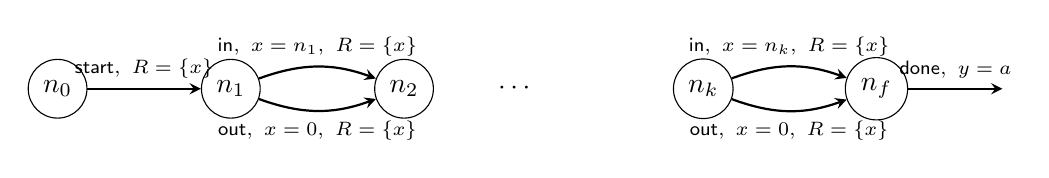
\begin{tikzpicture}[>=stealth, node distance=2.2cm, on grid, auto]

\tikzstyle{node}=[circle, draw, minimum size=7mm]
\tikzstyle{trans}=[->, thick]

\node[node] (n0) {$n_0$};
\node[node, right=of n0] (n1) {$n_1$};
\node[node, right=of n1] (n2) {$n_2$};
\node at ($(n2)+(1.4,0)$) {$\cdots$};
\node[node, right=3.8cm of n2] (nk) {$n_k$};
\node[node, right=of nk] (nf) {$n_f$};

\draw[trans] (n0) -- node[above] {\scriptsize $\mathsf{start},\ R=\{x\}$} (n1);

\draw[trans, bend left=20] (n1) to
node[above] {\scriptsize $\mathsf{in},\ x=n_1,\ R=\{x\}$} (n2);
\draw[trans, bend right=20] (n1) to
node[below] {\scriptsize $\mathsf{out},\ x=0,\ R=\{x\}$} (n2);

\draw[trans, bend left=20] (nk) to
node[above] {\scriptsize $\mathsf{in},\ x=n_k,\ R=\{x\}$} (nf);
\draw[trans, bend right=20] (nk) to
node[below] {\scriptsize $\mathsf{out},\ x=0,\ R=\{x\}$} (nf);

\draw[trans] (nf) -- node[above] {\scriptsize $\mathsf{done},\ y=a$} ++(1.6,0);

\end{tikzpicture}
\caption{Acyclic LTN encoding SUBSET-SUM. Clock $x$ is reset at every step and enforces a choice of delay 0 or $n_i$; clock $y$ accumulates total elapsed time and is checked at the final node.}
\label{fig:subset-sum-ltn}
\end{figure}

The drop from PSPACE (for general $k$-drift bounded LTNs) to NP (for acyclic LTNs) reflects the computational difference between verifying a semantic property versus exploiting a structural guarantee. In acyclic LTNs, the bound on run length provides additional structure that simplifies reachability analysis.

\section{Summary and Perspective}
\label{sec:drift-summary}

This chapter investigated \emph{drift}—the maximum divergence between agents' reference clocks—as both a source of undecidability and a unifying lens for understanding decidable fragments of local-timed negotiations.

\subsection*{Main Contributions}

\paragraph{Semantic restriction: drift boundedness.} We formalized an existential notion of $k$-drift boundedness (Definition~\ref{def:retiming-bounded}), requiring that every discrete behavior admit at least one timed realization with bounded clock divergence. This retiming-based notion, standard in timed automata theory, enables finite abstraction techniques.

\paragraph{Decidability via region abstraction.} For $k$-drift bounded LTNs, we adapted region-equivalence constructions from timed automata to obtain a finite $k$-region automaton (Section~\ref{sec:k-automaton}). This yielded PSPACE-completeness for location reachability (Theorem~\ref{thm:drift-pspace}), matching the complexity of timed automata despite the greater expressiveness of multi-agent interactions.

\paragraph{Structural implication: acyclicity.} We showed that acyclicity of the marking graph—a purely structural, efficiently checkable property—implicitly enforces bounded drift (Theorem~\ref{thm:acyclic-drift-bounded}). For acyclic LTNs, reachability drops to NP-complete (Theorem~\ref{thm:acyclic-np}), reflecting the added structure that simplifies verification.

\paragraph{Meta-complexity.} We established that verifying universal $k$-drift boundedness is PSPACE-complete (Proposition~\ref{prop:universal-k-decidable}), while determining the existence of a universal drift bound is undecidable (Proposition~\ref{prop:universal-undecidable}).

\subsection*{Conceptual Insights}

Three key insights emerge from this chapter:

\begin{enumerate}
\item \textbf{Drift as a unifying principle:} Unbounded drift enables counter encoding and undecidability, while bounded drift—whether enforced semantically or structurally—restores finite abstractions. Both synchronization extremes from Chapter~\ref{chap:fragments} can be understood as special cases where drift is controlled: synchronization-free LTNs trivialize drift by preventing clock comparisons, while always-synchronizing LTNs bound drift through constant resynchronization.

\item \textbf{Existential vs.\ universal:} The existential notion of drift boundedness (retiming-based) is weaker but more useful for verification than universal boundedness. It aligns with time-abstract verification and enables reasoning about discrete behaviors independently of specific timing choices.

\item \textbf{Syntax implies semantics:} Acyclicity provides a syntactic sufficient condition for the semantic property of drift boundedness. This connection is non-obvious—acyclicity constrains control flow but says nothing explicitly about timing—yet it guarantees bounded drift with a computable bound. This pattern suggests that other structural restrictions might similarly imply semantic boundedness properties.
\end{enumerate}

\subsection*{Broader Perspective}

From a broader perspective, this chapter highlights a fundamental trade-off in real-time concurrent systems: expressiveness arises from the combination of local autonomy (independent clocks), selective coordination (partial synchronization), and unbounded temporal evolution, while decidability is recovered by constraining how divergence accumulates across interactions.

The dichotomy between NP (acyclic) and PSPACE (general $k$-drift bounded) also reveals a computational spectrum: systems where boundedness is structurally guaranteed admit simpler verification than those where boundedness must be checked semantically. This suggests that identifying richer classes of structurally drift-bounded LTNs could yield practical decidable fragments.

\section{Coming Next: Connected Communication}
\label{sec:drift-next}

Acyclicity is a strong restriction: many natural systems exhibit cycles in their control structure while still maintaining disciplined patterns of communication and synchronization. The next chapter studies such systems through the notion of \emph{connectedly communicating local-timed negotiations}.

Connectedly communicating LTNs allow cycles in the marking graph but impose a structural constraint on how agents interact across these cycles. Intuitively, agents that diverge in time cannot later compare their clocks without passing through a communication path that enforces synchronization. This condition rules out the counter-encoding patterns responsible for undecidability while retaining significantly more expressive power than acyclic LTNs.

In Chapter~\ref{chap:connected-communication}, we show that connected communication suffices to bound drift and yields decidable reachability, thereby bridging the gap between purely semantic drift bounds (this chapter) and purely structural acyclicity. This completes our characterization of the decidability landscape for LTNs, delineating the boundary between tractable and intractable fragments based on the interplay of timing, synchronization, and interaction structure.
%\input{Chapter7-draft3}
%\input{Chapter8-draft1}
%\chapter{Conclusion and Future Directions}
\label{chap:conclusion}

\section{Conclusion}

Concurrent systems with quantitative timing constraints are pervasive in practice—from distributed protocols and embedded systems to cyber-physical infrastructures—yet modeling them presents fundamental tensions between expressiveness, compositionality, and decidability. This thesis introduced \emph{local-timed negotiations (LTNs)} as a unifying formalism that addresses these tensions by combining two complementary perspectives: the interaction-centric view of negotiations, which makes concurrency and causal structure explicit, and the quantitative timing framework of timed automata, which enables precise reasoning about real-time behavior.

The key innovation of LTNs lies in assigning clocks and timing constraints \emph{locally} to agents and interactions rather than globally. This locality principle captures timing phenomena—such as bounded desynchronization, partial observation of delays, and interaction-dependent progress—that are difficult to express cleanly in either negotiations or timed automata alone. At the same time, unrestricted locality leads quickly to undecidability, subsuming the power of networks of timed automata. The central question motivating this thesis is therefore: \emph{which natural restrictions on timing, synchronization, and structure suffice to recover decidability while preserving expressive power?}

\subsection*{Contributions and Main Results}

The thesis answers this question through a systematic exploration of the decidability landscape for LTNs, organized along three axes: synchronization patterns, clock divergence, and structural constraints.

\paragraph{Foundations.} After establishing the formal semantics of LTNs in Chapter~\ref{chap:ltn-definitions}, with careful attention to local clocks, joint occurrences, and monotonicity, the thesis positions LTNs as a strict generalization of untimed negotiations and a structured alternative to product constructions over timed automata. This foundation clarifies how timing information propagates through interactions and provides the technical basis for subsequent decidability results.

\paragraph{Extreme synchronization regimes.} Chapter~\ref{chap:sync-fragments} analyzes two opposite ends of the synchronization spectrum. In the \emph{synchronization-free} fragment, where timing constraints decouple across agents, a finite abstraction via product-region construction yields \PSPACE-completeness. At the other extreme, the \emph{always-synchronizing} fragment tightly couples agents through every interaction, yet every reachable configuration admits a monotone witness run, enabling a reduction to timed automata reachability—also \PSPACE-complete. These results establish baseline complexity bounds and demonstrate that both maximal independence and maximal dependence can be decidable when properly formalized.

\paragraph{Bounded desynchronization.} Between these extremes lies the conceptually rich territory of \emph{partial synchronization}. Chapter~\ref{chap:drift-bounded} introduces \emph{drift-bounded LTNs}, where local clocks may diverge but only within a bounded range. By adopting an existential notion of drift boundedness—requiring only that \emph{some} execution witnesses the target configuration with bounded drift—the thesis shows that decidability can be restored without requiring global synchronization. Crucially, acyclic LTNs are proven drift-bounded, with reachability shown to be \NP-complete (Theorem~\ref{thm:acyclic-np}). This result highlights \emph{bounded desynchronization} as a key semantic principle underlying decidability in timed interaction models.

\paragraph{Structural coherence.} Finally, Chapter~\ref{chap:connected-communication} explores structural restrictions that enforce global coherence without full synchronization. The notion of \emph{connectedly communicating LTNs} demonstrates how interaction topology can be exploited to refine decidability boundaries, complementing the semantic restrictions on drift and synchronization.

\subsection*{Conceptual Framework}

Beyond individual complexity results, this thesis contributes a conceptual framework for understanding the interplay between timing, synchronization, and structure in concurrent systems. Three recurring themes emerge:

\begin{enumerate}
\item \textbf{Locality vs.\ globality:} Decidability often hinges on whether timing information remains local or must be globally coordinated. The synchronization-free and drift-bounded fragments exploit locality, while the always-synchronizing fragment manages global coordination through tight coupling.

\item \textbf{Semantic vs.\ syntactic restrictions:} Existential drift boundedness is a semantic property (depending on reachable behaviors), yet it can be verified syntactically for acyclic structures. This interplay between semantic guarantees and syntactic sufficient conditions recurs throughout the thesis.

\item \textbf{Monotonicity and normal forms:} Many decidability proofs rely on constructing canonical witnesses—monotone runs, truncated configurations, or region-normalized executions—that preserve reachability while admitting finite representation. These proof techniques suggest deeper connections to well-quasi-orderings and well-structured systems.
\end{enumerate}

Taken together, the results delineate a rich landscape of timed interaction models and demonstrate that undecidability can be avoided through principled restrictions on how agents coordinate their timing behavior.

\section{Broader Directions and Outlook}
\label{sec:future-directions}

The framework of local-timed negotiations opens a broader research program centered on \emph{quantitative verification under structural constraints}. The decidable fragments and proof techniques developed in this thesis suggest multiple directions for extending both the theoretical foundations and practical applicability of LTNs. Below, we outline core continuations of this work, organized by increasing scope and ambition.

\subsection{Counting and Enumeration Problems}

The finite abstractions and normal-form constructions developed for decidable LTN fragments suggest natural extensions to \emph{counting problems}. Rather than asking whether a configuration is reachable, one can ask: \emph{how many} distinct executions reach it? Or: how many reachable configurations satisfy a given property?

For synchronization-free LTNs, the product-region construction of Chapter~\ref{chap:sync-fragments} provides a finite graph whose paths correspond to executions. This immediately yields decidability of counting reachable configurations. However, the complexity of \emph{exact counting} or \emph{approximate counting} remains open. Similarly, for always-synchronizing LTNs, the monotone witness runs established in Theorem~\ref{thm:always-sync-pspace} admit a finite representation, but whether this enables efficient counting is unclear.

A particularly compelling question concerns acyclic and drift-bounded LTNs (Chapter~\ref{chap:drift-bounded}). Since reachability is \NP-complete (Theorem~\ref{thm:acyclic-np}), natural follow-up questions include:
\begin{itemize}
\item Can reachable configurations be enumerated with polynomial delay?
\item Does counting reachable configurations remain in \#P, or does drift boundedness enable more efficient algorithms?
\item Can standard approximation techniques (e.g., FPRAS) be adapted to count executions up to clock-region equivalence?
\end{itemize}

Answering these questions would connect LTNs to the growing literature on counting and enumeration in verification and would clarify whether the semantic restrictions ensuring decidability also yield computational tractability for quantitative queries.

\subsection{Quantitative Extensions: Costs, Weights, and Counters}

Chapter~\ref{chap:ltn-definitions} deliberately restricts LTNs to clock constraints without accumulated quantitative effects such as costs or counters. A natural next step is to incorporate such features, enabling the study of resource-aware verification and optimization problems.

The drift-boundedness results of Chapter~\ref{chap:drift-bounded} are particularly suggestive here. Since decidability relies on bounding clock \emph{divergence} rather than absolute time, it is plausible that additive cost models or bounded counters could be incorporated without destroying decidability. Concretely:
\begin{itemize}
\item \textbf{Cost-annotated LTNs:} Associate integer costs with interactions and ask whether a target configuration is reachable with total cost below a threshold. Does existential drift boundedness suffice for decidability of cost-bounded reachability?
\item \textbf{Optimal reachability:} For always-synchronizing LTNs, can cost-optimal executions be found via reduction to priced timed automata?
\item \textbf{Counter extensions:} Allow agents to maintain integer counters (e.g., modeling resource counts) that are incremented or decremented during interactions. Do acyclic counter-LTNs preserve \NP-completeness, or does interaction with drift boundedness lead to undecidability?
\end{itemize}

These extensions would position LTNs as a framework for studying quantitative objectives in concurrent systems, bridging the gap between qualitative reachability analysis and optimization.

\subsection{Structural Parameters and Well-Structuredness}

Several results in this thesis point toward the importance of structure: acyclicity (Definition~\ref{def:acyclic-ltn}) and connected communication (Chapter~\ref{chap:connected-communication}) both impose global coherence without requiring full synchronization. However, these restrictions were introduced somewhat \emph{ad hoc}, motivated by specific decidability proofs rather than a systematic theory.

A more principled approach would be to study \emph{parametric structural restrictions} on LTNs and characterize their impact on decidability and complexity. Promising parameters include:
\begin{itemize}
\item \textbf{Interaction hypergraph structure:} Does bounding the treewidth, pathwidth, or treedepth of the negotiation hypergraph yield new decidable fragments or improved complexity bounds?
\item \textbf{Negotiation arity:} All results in this thesis apply to arbitrarily large interactions. Does restricting to binary or bounded-arity interactions simplify analysis or admit efficient algorithms?
\item \textbf{Hierarchical patterns:} Can layered or modular interaction structures—common in protocol design—be exploited for compositional verification?
\end{itemize}

More ambitiously, the monotonicity and truncation techniques used in Lemmas~\ref{lem:monotone-witness} and~\ref{lem:bounded-truncation} suggest connections to \emph{well-quasi-orderings} (WQOs) and well-structured transition systems (WSTS). An open problem is whether abstract LTN configurations can be equipped with a WQO that respects reachability, thereby importing the powerful termination and coverability results from the WSTS literature. Such a connection would situate LTNs within a broader theoretical framework and could yield generic decidability results for rich classes of timed interaction systems.

\subsection{Beyond Reachability: Broader Verification and Synthesis}

While reachability captures the core decidability challenges in LTNs, many verification problems remain unexplored:
\begin{itemize}
\item \textbf{Safety and liveness:} Can invariants or bounded-response properties be verified using the region-based abstractions from Chapter~\ref{chap:sync-fragments}?
\item \textbf{Quantitative specifications:} Can metric temporal logic or timed logics be model-checked over decidable LTN fragments?
\item \textbf{Parametric verification:} Given a family of LTNs parameterized by timing constants, can one synthesize constraints ensuring reachability or drift boundedness?
\end{itemize}

The explicit interaction structure of LTNs also suggests new \emph{synthesis} questions. For instance: given a partial specification of interactions and timing constraints, can one automatically complete it to ensure drift boundedness or enforce timely synchronization? Such problems extend the reachability analysis toward controller synthesis, where the goal is to construct strategies that guarantee desired timing properties in the presence of environmental uncertainty or adversarial agents.

\subsection{Connections to Other Infinite-State Models}

The expressiveness results implicit throughout this thesis—particularly the undecidability proofs that motivate restrictions—call for a deeper comparison between LTNs and other infinite-state concurrency models. While Chapter~\ref{chap:ltn-definitions} positions LTNs as a synthesis of negotiations and timed automata, precise translations to related models remain open:
\begin{itemize}
\item \textbf{Timed Petri nets:} How do LTNs compare to time Petri nets or timed-arc Petri nets in expressiveness? Can drift boundedness be related to boundedness in Petri nets?
\item \textbf{Communicating timed automata:} Networks of timed automata with message passing are known to be undecidable. Can the restrictions ensuring decidability in LTNs be translated to communication protocols, and vice versa?
\item \textbf{Negotiation-VASS:} Untimed negotiations with counters have been studied recently. Can the techniques from LTNs inform decidability boundaries when both timing and counting are present?
\end{itemize}

Understanding these connections would clarify the relative power of LTNs and reveal whether principles like drift boundedness and structural coherence apply broadly across infinite-state models.

\subsection{Toward Practical Modeling and Tool Support}

Finally, LTNs suggest a modeling paradigm closely aligned with how distributed protocols are described in practice: via explicit interactions and local timing constraints rather than monolithic global states. This raises the question of whether LTNs can serve as a practical specification language.

A concrete direction is to develop \emph{prototype tool support} for LTNs, targeting the decidable fragments identified in this thesis:
\begin{itemize}
\item Implement verification algorithms for acyclic and drift-bounded LTNs (Chapter~\ref{chap:drift-bounded}).
\item Build abstraction-based model checkers for synchronization-free and always-synchronizing fragments (Chapter~\ref{chap:sync-fragments}).
\item Explore heuristic or approximate methods for more general LTNs, using drift boundedness as a runtime check.
\end{itemize}

Such tools would enable empirical evaluation on case studies drawn from distributed protocols, embedded systems, or cyber-physical applications. They could also guide the discovery of additional restrictions motivated by real-world modeling needs, creating a feedback loop between theory and practice.

\section*{Closing Remark}

Local-timed negotiations were introduced in this thesis not as an isolated formalism, but as a lens through which concurrency and time can be studied together at the level of \emph{interaction}. The decidability landscape charted here reveals that this lens is productive: it exposes new decidable classes, clarifies fundamental boundaries, and illuminates the subtle interplay between local autonomy and global coordination in real-time concurrent systems.

Yet this thesis represents only a beginning. The future directions outlined above—spanning counting, costs, structure, synthesis, and tool support—collectively point toward a broader research program on \emph{quantitative and structural verification of interaction systems}. Such a program naturally aligns with current trends in formal methods, from parametric verification and well-structured systems to quantitative synthesis and resource-aware logics. It offers multiple entry points for both theoretical advances—connecting LTNs to established frameworks like WSTS or extending them with richer quantitative features—and practical applications in protocol analysis and embedded system design.

It is my hope that local-timed negotiations will serve not only as a theoretical contribution to the foundations of timed concurrency, but also as a generative framework—one that inspires new questions, enables new techniques, and ultimately deepens our understanding of how time, interaction, and structure shape the behavior of concurrent systems.

\appendix

\bibliography{references}
\bibliographystyle{alpha}

\end{document}